\documentclass{style/these}
\usepackage[T1]{fontenc}
\usepackage[utf8]{inputenc}

\usepackage{titletoc}					% parttoc on part title

\usepackage{float}
\usepackage{graphicx}
\usepackage{xcolor}
\usepackage{tcolorbox} 
\usepackage{afterpage}

\usepackage{amssymb}
\usepackage{amsmath}
\usepackage{nicefrac}

\usepackage{multirow} 
\usepackage[normalem]{ulem}

\usepackage[backend=bibtex,style=authoryear,sorting=nyt,firstinits=true,maxnames=2,maxbibnames=10,bibencoding=ascii]{biblatex}
 

\usepackage[unicode=true,pdfusetitle,
	    colorlinks=true,linkcolor=black,urlcolor=black,citecolor=darkerblue,pdftex,linktocpage=true,hyperindex=true,
            bookmarks=true,bookmarksnumbered,bookmarksopen=false,breaklinks=false,
            backref=true,pdfstartview={FitH},pdfpagemode={UseOutlines}, pdfborder={0 0 1}]{hyperref}
            
\usepackage[titletoc,title]{appendix}
\usepackage[french,tight]{minitoc}

\usepackage{lipsum}
\usepackage{bookmark}
\usepackage[acronym,nonumberlist,nomain]{glossaries}

\usepackage[shorthands=;!?]{babeltools}
\usepackage[english,french]{babel}

\usepackage{setspace}						% change line spacings

\usepackage[justification=centering]{caption}			% centered captions for figures and tables
\usepackage{subcaption}						% subtable & subfigure

\usepackage[section]{placeins}					% figures in corresponding sections

\usepackage{tipa}						% IPA phonetic symbols

\usepackage{algorithm}
\usepackage[noend]{algpseudocode}

\usepackage{colortbl}						% color in hline

\renewcommand\familydefault{ptm}


%==================================================
% Données
%==================================================

\author{Luiza Orosanu}
\title{Reconnaissance de la parole\\ pour l'aide à la communication\\ pour les sourds et malentendants}
\date{11 Décembre 2015}


%==================================================
% Définitions
%==================================================

%\captionsfrench

\definecolor{darkblue}{RGB}{0,0,139}
\definecolor{darkerblue}{RGB}{0,0,120}
\definecolor{royalbleu}{RGB}{0,35,102}
\definecolor{blendedblue}{rgb}{0.137,0.466,0.741}
\definecolor{OrangeRed}{RGB}{255, 40, 0}
\definecolor{darksalmon}{RGB}{233,150,122}
\definecolor{maroon}{rgb}{0.665, 0.142, 0.142}
\definecolor{lightergray}{RGB}{220,220,220}
\definecolor{darkgreen}{RGB}{0,128,0}

\newenvironment{fbookman}{\fontfamily{pbk}\fontseries{x}\footnotesize\selectfont}{\par}
\newenvironment{nbookman}{\fontfamily{pbk}\fontseries{x}\selectfont}{\par}
\newenvironment{lnbookman}{\fontfamily{pbk}\fontseries{x}\large\selectfont}{\par}
\newenvironment{Lbookman}{\fontfamily{pbk}\fontseries{bx}\Large\selectfont}{\par}
\newenvironment{Lnbookman}{\fontfamily{pbk}\fontseries{x}\Large\selectfont}{\par}
\newenvironment{LLbookman}{\fontfamily{pbk}\fontseries{bx}\LARGE\selectfont}{\par}
\newenvironment{LLnbookman}{\fontfamily{pbk}\fontseries{x}\LARGE\selectfont}{\par}
\newenvironment{Hbookman}{\fontfamily{pbk}\fontseries{bx}\Huge\selectfont}{\par}

\newcommand{\hilight}[1]{\colorbox{lightergray}{#1}}

\renewcommand{\ULthickness}{1.6pt}

\newcolumntype{L}[1]{>{\raggedright\let\newline\\\arraybackslash\hspace{0pt}}m{#1}}		%Left-align column
\newcolumntype{C}[1]{>{\centering\let\newline\\\arraybackslash\hspace{0pt}}m{#1}}		%Center-align column
\newcolumntype{R}[1]{>{\raggedleft\let\newline\\\arraybackslash\hspace{0pt}}m{#1}}		%Right-align column

\newcommand\fnurl[2]{%
  \href{#2}{#1}\footnote{\url{#2}}%
}

% new line after paragraph
\newcommand{\myparagraph}[1]{\subparagraph{#1}\vskip-.2cm \mbox{}\\\vskip-.2cm}

% add blank page
\newcommand\blankpage{%
    \null
    \thispagestyle{empty}%
    \addtocounter{page}{-1}%
    \newpage}
   
% remove double blank page  
\makeatletter
\renewcommand*{\cleardoublepage}{\clearpage\if@twoside \ifodd\c@page\else
	\hbox{}%
	\thispagestyle{empty}%
	\newpage%
	\if@twocolumn\hbox{}\newpage\fi\fi\fi}
\makeatother

% remove page number from part
\makeatletter
\renewcommand\part{%
  \if@openright
    \cleardoublepage
  \else
    \clearpage
  \fi
  \thispagestyle{empty}%   % Original »plain« replaced by »empty
  \if@twocolumn
    \onecolumn
    \@tempswatrue
  \else
    \@tempswafalse
  \fi
  \null\vfil
  \secdef\@part\@spart}
\makeatother

 
% change font in tables
\makeatletter
\newenvironment{aTable}%
  {%\renewcommand\normalsize{\small}\normalsize
   \renewcommand{\familydefault}{lmtt}\selectfont
  \@float{table}}
  {\end@float}
\makeatother

% change font in tables
\makeatletter
\renewenvironment{table}%
{ \renewcommand{\familydefault}{ptm}\selectfont
  \@float{table}}
  {\end@float}
\makeatother

%split line in table cell
\newcommand{\specialcell}[2][r]{%
  \begin{tabular}[#1]{@{}r@{}}#2\end{tabular}}
  

%=======================================
% TOC 
%=======================================

\setcounter{tocdepth}{3}
%\setcounter{secnumdepth}{3}
%\setcounter{parttocdepth}{1} 

\makeatletter
\let\stdl@part\l@part
\renewcommand*{\l@part}[2]{%
  \stdl@part{\textcolor{darkblue}{#1}}{\textcolor{darkblue}{#2}}}
\makeatother

% restart each part with capter 1
%\makeatletter
%\@addtoreset{chapter}{part}
%\makeatother  

\newcommand{\newchapter}[1]{%
    \chapter*{#1}
    \addcontentsline{toc}{chapter}{%
        \hspace{-39pt} \textbf{\large #1}
    }
}

\newcommand{\newsection}[1]{%
    \section*{#1}
    \addcontentsline{toc}{section}{%
        \hspace{-39pt} #1}
}

\newcommand{\hiddensection}[1]{
    \stepcounter{section}
    \subsection*{\arabic{chapter}.\arabic{section}\hspace{1em}{#1}}
}

\newcommand{\hiddensubsection}[1]{
    \stepcounter{subsection}
    \subsection*{\arabic{chapter}.\arabic{section}.\arabic{subsection}\hspace{1em}{#1}}
}


%increase size between number and caption for listoffigure
\makeatletter
     \renewcommand*\l@figure{\@dottedtocline{1}{1em}{2.6em}}
\makeatother

%\makeatletter
%\renewcommand{\p@chapter}{\thepart.}
%\makeatother

%\makeatletter
%\renewcommand{\p@section}{\thepart.\thechapter.}
%\makeatother

%============================================================
% spaces between chapter/section/subsection in TOC
%============================================================

\makeatletter
\pretocmd{\part}{\addtocontents{toc}{\protect\addvspace{12\p@}}}{}{}		%16
\pretocmd{\chapter}{\addtocontents{toc}{\protect\addvspace{9\p@}}}{}{}		%12
\pretocmd{\section}{\addtocontents{toc}{\protect\addvspace{5\p@}}}{}{}		%8
\pretocmd{\subsection}{\addtocontents{toc}{\protect\addvspace{2\p@}}}{}{}	%3
\makeatother

  
\makeatletter
%\renewcommand*\l@part{\@dottedtocline{1}{1em}{2.3em}}
\renewcommand*\l@chapter{\@dottedtocline{1}{3em}{1.6em}}
\renewcommand*\l@section{\@dottedtocline{1}{5.7em}{2.3em}}
\renewcommand*\l@subsection{\@dottedtocline{1}{7em}{2.0em}}
\makeatother  

%=============================================
% glossaries
%=============================================

\renewcommand*{\glstextformat}[1]{#1}
%\renewcommand*{\glstextformat}[1]{\color{darkgray} #1}
%\renewcommand*{\glstextformat}[1]{\color{darkgray}\textit{#1}}
%\renewcommand*{\glstextformat}[1]{\contour{black}{\textcolor{black}{#1}}}
%\renewcommand*{\glstextformat}[1]{\color{darkgreen}\textbf{#1}} %\underline{\emph{#1}}}

\makeglossaries

%=============================================
% parttoc on the Part title page
%=============================================

\makeatletter
\def\@endpart{
\vfil
\textcolor{darkblue}{\hrule height 1.6 pt}
\setcounter{tocdepth}{1}

\startcontents[parts]
\printcontents[parts]{}{0}{}

\textcolor{darkblue}{\vskip-2ex\hrule height 1.6 pt}
\par\bigskip
\vfil\newpage
}
\makeatother


% table and figure number in parts

%\numberwithin{figure}{part}
%\numberwithin{table}{part}

%==============================================
% bibliography
%==============================================

\DeclareCiteCommand{\cite}
  {\usebibmacro{prenote}}
  {\usebibmacro{citeindex}%
   \printtext[bibhyperref]{\usebibmacro{cite}}}
  {\multicitedelim}
  {\usebibmacro{postnote}}

\addbibresource{biblio/general}
\addbibresource{biblio/myPub}

\let\oldcite=\cite
\renewcommand{\cite}[1]{{\fontfamily{qcs}\selectfont{\color{darkerblue}[\oldcite{#1}]}}}

%\renewcommand{\cite}[1]{{{\color{darkerblue}[\oldcite{#1}]}}}
%\renewcommand{\cite}[1]{{\fontfamily{qbk}\selectfont{\color{darkerblue}[\oldcite{#1}]}}}
%\renewcommand{\cite}[1]{{\fontfamily{lmr}\selectfont{\color{darkerblue}[\oldcite{#1}]}}}
%\renewcommand{\cite}[1]{{\fontfamily{lmr}\fontseries{bx}\selectfont{\color{darkerblue}[\oldcite{#1}]}}}

%\renewcommand{\multicitedelim}{\addsemicolon\space}

%==================
% algorithm
%==================

\DeclareCaptionFormat{myformat}{#3}
\captionsetup[algorithm]{format=myformat}

\makeatletter
\def\BState{\State\hskip-\ALG@thistlm}
\makeatother


% minitoc depth ...
\setcounter{minitocdepth}{4}


\newcolumntype{g}{>{\color{gray}}l}
\newcolumntype{b}{>{\color{black}}l}


%%%%%%%%%%%%%%%%%%%%%%%%%%%%%%%%%%%%%%%%%%%%%%%%%%%%%%%%%%%%%%%%%%%%%%%%%%%%
% Begin ...
%%%%%%%%%%%%%%%%%%%%%%%%%%%%%%%%%%%%%%%%%%%%%%%%%%%%%%%%%%%%%%%%%%%%%%%%%%%%



\begin{document}

\pagestyle{empty}

\frontmatter

\maketitle

%==================================================
\vspace*{50px}
\begin{center}\section*{Remerciements}\end{center}
%==================================================
\phantomsection


\vskip1cm
{
\setstretch{1.4}


Mes premiers remerciements vont à mon directeur de thèse, M. Denis Jouvet, qui m'a soutenu et encouragé tout au long de cette thèse. 
Ses compétences, ses conseils et ses remarques ont été d'une aide précieuse pour faire avancer mes recherches. 
J'ai pu également apprécier sa gentillesse et sa disponibilité malgré son emploi du temps plus que chargé. 
Je suis très reconnaissante pour toutes les corrections, recorrections et rerecorrections de ce document.

\vskip1ex
Je remercie également les membres de l'entreprise eROCCA pour m'avoir donné l'occasion de travailler sur leur projet.

\vskip1ex
Je souhaite également remercier l'ensemble de l'équipe Multispeech pour m'avoir fourni un cadre de travail enrichissant et agréable.

\vskip1ex
Enfin, j'aimerais remercier mon petit ami, Luc, pour sa compréhension, son soutien et son aide tout au long de mon travail.

}


\afterpage{\blankpage}
\newpage

%==================================================
\section*{Résumé}
%==================================================
\phantomsection

\vspace{0.5ex}

{
\setstretch{1.02}
Le projet  RAPSODIE \fnurl{}{http://erocca.com/rapsodie} a été lancé en 2012 avec l'objectif de développer une nouvelle génération de terminaux proposant une reconnaissance vocale spécialisée sur les besoins des personnes sourdes ou malentendantes. Dans ce contexte, l'objectif de cette thèse est d'étudier, d'approfondir et d'enrichir l'extraction d'informations lexicales et para-lexicales à partir de la parole pour aider à la communication avec des personnes sourdes ou malentendantes. 

En ce qui concerne la modélisation lexicale, nous nous sommes intéressés au choix des unités lexicales définissant le lexique et au modèle de langage associé. 
L'optimisation du décodage phonétique nous a conduit à évaluer différentes unités lexicales, comme les phonèmes et les mots, et à proposer l'utilisation des syllabes. 
Cependant, des entretiens effectués en parallèle avec des personnes sourdes ont révélé l'intérêt d'une reconnaissance en mots qui est plus simple à appréhender et qui ne nécessite pas d'effort supplémentaire de la part du lecteur pour regrouper les différentes phonèmes ou syllabes en mots porteurs de sens. 
Cela nous a amenés à proposer une nouvelle approche reposant sur la combinaison de mots et de syllabes dans un seul modèle de langage, dit hybride. 
L'utilisation d'un tel modèle de langage hybride vise à assurer une reconnaissance correcte des mots les plus fréquents et à proposer des suites de syllabes pour les segments de parole correspondant à des mots hors vocabulaire. 
 
Afin d'assurer une bonne reconnaissance des mots spécifiques à un certain domaine, nous avons approfondi l'ajout de nouveaux mots dans le modèle de langage sans faire de ré-apprentissage ni d'adaptation du modèle de langage (qui sont des traitements qui nécessitent beaucoup de données). 
Nous avons donc proposé et évalué une nouvelle approche pour l'ajout de mots qui repose sur un principe de similarité entre mots. 
Deux mots sont considérés comme similaires  s'ils ont des distributions similaires de leurs voisins; formellement, cela se traduit par un calcul de divergence entre les distributions des mots prédécesseurs et des mots successeurs.
L'approche implique ainsi plusieurs étapes : utiliser quelques phrases exemples pour le nouveau mot à ajouter, chercher dans le modèle de langage des mots similaires au nouveau mot, puis définir les n-grammes associés à ce nouveau mot à partir des n-grammes des mots similaires.

Concernant l'extraction d'informations para-lexicales, nous nous sommes intéressés principalement à la détection des questions et des affirmations. Cette détection vise à enrichir la communication avec les personnes sourdes ou malentendantes, de manière à leur signaler quand une question leur est adressée, afin qu'ils puissent y répondre ou intervenir par une demande de répétition ou de clarification. 
Dans notre étude, plusieurs approches ont été analysées utilisant respectivement seulement des paramètres prosodiques (extraits du signal audio), seulement des paramètres linguistiques (extraits des séquences de mots et de classes grammaticales), ou combinant les deux types d'information. 
L'évaluation de classifieurs est effectuée en utilisant des paramètres linguistiques et prosodiques extraits à partir de transcriptions automatiques (pour étudier la performance dans
des conditions réelles) et de transcriptions manuelles (pour étudier la performance dans des conditions idéales). 
L'impact d'erreurs sur les frontières des phrases a également été étudié. 
}

\vspace{1.5ex}

\noindent\textbf{Mots clés} : reconnaissance de la parole, syllabes, modèles de langage hybrides, mots hors-vocabulaire,  mots similaires, détection de questions


%\afterpage{\blankpage}
\cleardoublepage


%==================================================
\section*{Abstract}
%==================================================
\phantomsection

\vspace{0.5ex}

{
\setstretch{1.02}
The RAPSODIE \fnurl{}{http://erocca.com/rapsodie} project was launched in 2012 with the objective of proposing a speech recognition device specialized on the needs of deaf and hearing impaired people. 
In this context, the aim of the thesis is to study, deepen and enrich the extraction of lexical and para-lexical information from speech in order to help communication with deaf and hearing impaired people.

Regarding the lexical modeling, we focused on optimizing the choice of lexical units (defining the vocabulary and the associated language model). 
The optimisation of the phonetic decoding led us to evaluate various lexical units, such as phonemes and words, and to propose the use of syllables. 
However, the interviews conducted in parallel with deaf people showed interest in a word-based recognition, which is the easiest to understand and it does not require additional effort for the reader in order to group up different phonemes or syllables into meaningful words. 
This led us to propose a new approach based on the combination of words and syllables into a hybrid language model. 
The use of this hybrid language model aims to ensure proper recognition of the most frequent words and to offer sequences of syllables for speech segments corresponding to out-of-vocabulary words.
 
In order to ensure proper recognition of specific words in a certain area, we have focused on adding new words into the language model, without re-training or adapting the language model (treatments that require a lot of new data). 
We have therefore proposed and evaluated a new approach to adding words into the model based on a principle of similarity between words. 
Two words are considered as similar if they have similar neighbors distributions; formally, this results in the computation of the KL divergence on the distribution of their neighbor words. 
The approach involves three steps: defining a small set of sentences containing the new word to be added, looking for in-vocabulary words similar to the new word, defining the n-grams associated with the new word based on the n-grams of its similar in-vocabulary words.

Regarding the extraction of para-lexical information, we focused mainly on the detection of questions and statements. 
This detection aims to enhance communication with deaf and hearing impaired people, in order to inform them when a question is addressed to them because they have to respond or demand a repetition or a clarification. 
In our study, several approaches were analyzed using only prosodic features (extracted from the audio signal), only linguistic features (extracted from word sequences and sequences of POS tags), or combining both types of information. 
The evaluation of the classifiers is performed using linguistic and prosodic features (alone or in combination) extracted from automatic transcriptions (to study the performance under real conditions) and from manual transcriptions (to study the performance in ideal conditions). 
The performance loss when sentence boundaries are not perfect was also evaluated.


\vspace{1.5ex}

\noindent\textbf{Keywords}: speech recognition, syllables, hybrid language models, out-of-vocabulary words, similar words, question detection
}

\cleardoublepage
%\afterpage{\blankpage}

%==================================================
\dominitoc
\doparttoc

\tableofcontents

\addtocontents{toc}{\protect\thispagestyle{empty}}


%list of figures
\cleardoublepage
\begingroup
\makeatletter
\let\ps@plain\ps@empty
\makeatother

\pagestyle{empty}
{\small \listoffigures}
\cleardoublepage
\endgroup

%list of tables
\cleardoublepage
\begingroup
\makeatletter
\let\ps@plain\ps@empty
\makeatother

\pagestyle{empty}
{\small \listoftables}
\cleardoublepage
\endgroup


%==================================================

\mainmatter

\pagestyle{fancy}

\setstretch{1.08}
%\doublespacing														% comment after



%\fontfamily{cmr}\fontseries{sb}\selectfont
%\fontfamily{ptm}\fontseries{c}\selectfont
%\usefont{T1}{cmr}{m}{n}
%\fontfamily{ptm}\selectfont
\usefont{T1}{ptm}{m}{n}

%%%%%%%%%%%%%%%%%%%%%%%%%%%%%%%%%%%%%%%%%%%%%%%%%%%%%%%%%%%%%%%%%%%%%%%%%%%%
\chapter*{Introduction générale}
\renewcommand{\leftmark}{Introduction générale}
\addstarredchapter{\large Introduction générale}
%%%%%%%%%%%%%%%%%%%%%%%%%%%%%%%%%%%%%%%%%%%%%%%%%%%%%%%%%%%%%%%%%%%%%%%%%%%%

\minitoc

%==================================================================================
\section*{Contexte}
\renewcommand{\rightmark}{Contexte}
\addcontentsline{toc}{section}{\hspace{-39pt} Contexte}
%==================================================================================

La parole est le mode de communication le plus naturel. 
Grâce à elle nous pouvons donner une voix à notre volonté et à nos pensées. 
Nous pouvons l'utiliser pour exprimer des opinions, des idées, des sentiments, des désirs ou pour échanger, transmettre, demander des informations. 
Et aujourd'hui, nous ne l'utilisons pas uniquement pour communiquer avec d'autres humains, mais aussi avec des machines. 

La reconnaissance de la parole est la technique qui permet l'analyse des sons captés par un microphone pour les transcrire sous forme d'une suite de mots exploitables par les machines. 
Depuis son apparition dans les années 1950, la reconnaissance automatique de la parole a été constamment améliorée avec l'aide des phonéticiens, linguistes, mathématiciens et ingénieurs, qui ont définit les connaissances acoustiques et linguistiques nécessaires pour bien comprendre la parole d'un humain.
Cependant, les performances atteintes ne sont pas parfaites et dépendent de nombreux critères.
Les conditions favorables pour la reconnaissance de la parole impliquent une parole native, appartenant à un seul locuteur ayant une diction propre (ne présentant pas une pathologie de voix), enregistrée dans un environnement calme et non bruité, basée sur un vocabulaire commun (mots connus par le système). 
La performance du système diminue lorsque l'on traite des accents non-natifs, différents dialectes, des locuteurs qui présentent une pathologie de voix, des mots inconnus par le système (généralement des noms propres), des signaux audio bruités (faible rapport signal-à-bruit), etc.

Les applications de la reconnaissance de la parole sont très diversifiées et chaque système a sa propre architecture et son propre mode de fonctionnement. Plus le domaine d'application est vaste, plus les modèles de reconnaissance doivent être grands (pour pouvoir comprendre les discours spontanés et la diversité des locuteurs). 
De nos jours, de nombreuses recherches sur la reconnaissance de la parole sont effectuées dans le seul but d'imiter un assistant personnel : chercher des informations sur internet, noter des rendez-vous, envoyer des sms, contrôler différents équipements de la maison, etc. Mais très peu de recherches s'intéressent au bien-être de personnes handicapées, en particulier aux personnes sourdes ou malentendantes.

%==================================================================================
\section*{Problématique}
\renewcommand{\rightmark}{Problématique}
\addcontentsline{toc}{section}{\hspace{-39pt} Problématique}
%==================================================================================

L'entreprise eROCCA a lancé en 2012 le projet RAPSODIE \footnote{http://erocca.com/rapsodie/} (\textbf{R}econnaissance \textbf{a}uto-  \linebreak matique de la \textbf{p}arole pour les personnes \textbf{so}urdes ou han\textbf{di}capé\textbf{e}s) pour développer une nouvelle génération de terminaux proposant la reconnaissance vocale (initialement prévue en mode embarqué) dans le but d'améliorer la communication entre les sourds et leur entourage proche (dans la sphère privée ou professionnelle). 
La contrainte d'une reconnaissance embarquée a par la suite été relâchée au profit d'une implémentation en mode serveur.  
La liste des partenaires comprend le CEA - spécialisé dans les nanotechnologies, Castorama - magasin de bricolage avec une forte politique d'emploi des personnes handicapées (fournissant les conditions d'évaluation dans une situation réelle de travail) et INRIA - spécialisé dans la reconnaissance de la parole. 

Partie intégrante du projet RAPSODIE, les travaux réalisés dans cette thèse concernent la génération des transcriptions automatiques de la parole, avec un affichage adapté aux personnes sourdes. Les solutions proposées dans notre étude ont dû prendre en considération différentes contraintes imposées sur le mode de fonctionnement du système de reconnaissance (contexte initial embarqué), ainsi que les résultats des entretiens effectués dans le projet avec des personnes sourdes (concernant l'affichage des transcriptions) et tenir compte du contexte applicatif (magasin de bricolage).

Les partenaires du projet ont choisi d'utiliser les outils Sphinx3 et PocketSphinx pour le décodage de la parole, en raison de leur applicabilité en système embarqué (ces outils ajoutent une nouvelle contrainte sur les modèles de langage qui ne peuvent être que de type trigramme).

\myparagraph{Mode de fonctionnement}

Les contraintes imposées sur le système de reconnaissance automatique de la parole dépendent du mode de fonctionnement : embarqué (en local) ou mis en œuvre sur des serveurs (à distance). 
Dans le cas de reconnaissance à distance, l'enregistrement de la voix (fait sur un appareil) est envoyé (via le réseau) à des serveurs situés souvent à plusieurs centaines ou milliers de kilomètres. C'est là que de puissants ordinateurs vont transformer la parole en texte, qui va être ensuite renvoyé (via le réseau) à l'appareil. Cette solution assure la meilleure précision de reconnaissance aujourd'hui (grâce à l'utilisation d'importantes puissances de calcul et à des modèles appris sur de grosses bases de données), mais c'est cet aller-retour qui rend la reconnaissance vocale sur la plupart des appareils lente (en particulier sur les connexions cellulaires les plus lentes). De plus, il est impossible de l'utiliser hors-ligne. 
D'autre coté, les systèmes embarqués sont contraints par les ressources disponibles sur l'appareil : une capacité mémoire limitée et une puissance de calcul limitée. Mais ils ont l'avantage d'être accessibles à tout moment, sans être dépendants d'internet ou de serveurs distants. 
En conséquence, un système de reconnaissance automatique de la parole entièrement embarqué doit utiliser des modèles de reconnaissance assez performants (pour assurer la satisfaction de ses utilisateurs), mais en même temps assez petits, pour répondre aux contraintes de mémoire et de calcul, et générer des réponses rapides. 

\textit{Compte tenu du contexte initial embarqué du système de reconnaissance automatique de la parole, nous avons choisi d'effectuer une étude et une analyse détaillée sur la performance de différents modèles ``compacts''. Nous avons considéré en particulier le choix des unités lexicales pour obtenir le meilleur compromis entre le coût de calcul et l'utilisabilité des résultats. }

\myparagraph{Contexte de la surdité}

Le défi est de répondre aux besoins des personnes sourdes, ce qui implique une prise en compte de leurs habitudes, de leurs modes de communication, de leur savoir-faire et des problèmes qu'elles rencontrent au quotidien. Mais pour savoir comment aider les personnes sourdes, il faut d'abord comprendre leur ``handicap'' et leur histoire. 

Dans le passé, l'on pensait que les personnes qui ne pouvaient pas entendre ne pouvaient pas comprendre \cite{Moore:2013}.
Leur image a commencé à changer seulement à partir des années 1500, quand les premières langues de signes apparaissent \cite{Lane:1996}.   
En France, la première personne qui s'est intéressée aux personnes sourdes est Charles Michel De l'Épée en 1760. 
Il est le fondateur de la première école gratuite pour les sourds, et ses méthodes d'apprentissage sont basées sur l'utilisation de gestes naturels pour coder l'alphabet français mais aussi pour s'exprimer avec l'aide de gestes naturels selon la syntaxe du français \cite{Epee:1776, Epee:1784}. 
Son modèle a été suivi par d'autres pays et plusieurs méthodes d'apprentissage pour les sourds ont été inventées ultérieurement (en utilisant la langue de signes, la lecture labiale ou l'oralisme). 
Le temps passe et les entendants continuent à envisager les personnes sourdes comme des personnes handicapées, qui ont besoin d'aide pour devenir ``moins sourdes''. 
Mais toutes les personnes sourdes ne se considèrent pas comme étant handicapées, mais plutôt comme appartenant à une culture à part, basée sur la ``langue des sourds''. 
La langue de signes a été interdite aux personnes sourdes pendant une centaine d'années en France (entre 1880 et 1977). Ils ont été forcés à oraliser, c'est-à-dire à apprendre comment parler (sans même entendre) en utilisant la lecture labiale et en imitant les mouvements de la bouche et les modes de respiration. Mais la réussite de cette méthode dépend de plusieurs facteurs : du profil de la surdité, du milieu familial, de la méthode d'éducation choisie, de la rééducation, des appareillages et de l'âge de l'appareillage. 
Certaines personnes sourdes ne pourront jamais oraliser de façon compréhensible, ce qui s'est traduit par une forte augmentation du taux des sourds illettrés durant cette période. 
De nos jours, les personnes sourdes ont appris à utiliser tous les types d'information disponibles afin de pouvoir comprendre et communiquer : le langage corporel, la lecture labiale, la langue de signes et la langue française. Certains d'entre eux savent lire, écrire et même parler. Malgré tous les efforts d'adaptation au monde des entendants, il y aura toujours de grandes différences entre la vie d'un ``entendant'' et la vie d'un ``sourd''. Il y a beaucoup de problèmes simples pour un entendant, mais compliqués pour une personne sourde. Elles ont souvent du mal à trouver un emploi, à l'exercer et à le garder. C'est pour ça, et plus encore, que beaucoup des personnes sourdes se sentent exclues du monde des entendants \cite{Virole:1999, Delaporte:2002}.

La reconnaissance automatique de la parole pourrait apporter une compensation à ce handicap. Une transcription automatique pourrait aider les personnes sourdes à mieux comprendre leur entourage ou une émission de télévision ou une vidéo sur internet et cela sans faire aucun excès de concentration, sans se sentir gêné et sans avoir besoin d'un interprète de la langue de signes. 
La seule, mais importante, condition sera d'avoir une bonne maîtrise du français écrit (pour pouvoir comprendre la transcription automatique). 

\textit{Pour répondre à ce défi, nous nous sommes intéressés à l'extraction d'informations lexicales et para-lexicales à partir de la parole pour aider à la communication avec des personnes
sourdes ou malentendantes. }

%====================================================================
\section*{Plan du document}
\renewcommand{\rightmark}{Plan du document}
\addcontentsline{toc}{section}{\hspace{-39pt} Plan du document}
%====================================================================

Ce document est constitué de trois grandes parties.

La première partie présente les systèmes de reconnaissance de la parole. 
Tout d'abord, nous rappelons leur historique et nous donnons quelques exemples d'applications qui mettent en avant leur utilité pour aider les personnes handicapées. 
L'architecture des systèmes automatiques de reconnaissance de la parole est également présentée, avec la paramétrisation du signal et les modèles de reconnaissance associés. 
Nous détaillons les modèles et les techniques d'apprentissage utilisés dans nos travaux (modèles de langage n-grammes, modèles acoustiques \acrshort{HMM}-\acrshort{GMM}), et présentons brièvement les autres. 
La description du processus de reconnaissance complète cette partie, avec l'algorithme de décodage, l'évaluation des performances et l'utilité des mesures de confiance.  

La deuxième partie porte sur les aspects de modélisation lexicale. 
Nous nous sommes intéressés premièrement à la comparaison de différentes approches de décodage phonétique. 
Différentes unités lexicales ont été évaluées, comme les phonèmes et les mots, et nous avons proposé l'utilisation des syllabes. 
Nous avons ensuite proposé une approche de modélisation hybride, basée sur un lexique combinant mots et syllabes, pour permettre la reconnaissance des mots les plus fréquents, et l'affichage de mots hors vocabulaire sous forme de suites de syllabes. 
Pour répondre au besoin d'ajouter de nouveaux mots dans le modèle de langage, dans le but d'assurer une bonne reconnaissance de mots spécifiques à un certain domaine, une nouvelle approche basée sur un principe de similarité entre mots a été proposée et étudiée. 

La troisième partie porte sur l'extraction d'informations complémentaires, para-\linebreak lexicales, importantes pour la communication inter-personnes. 
Nous nous sommes intéressés principalement à la détection des questions et des affirmations, visant a enrichir la communication avec les personnes sourdes ou malentendantes, de manière à leur signaler quand une question leur à été adressée, car, dans ces cas, ils doivent répondre ou demander des précisions supplémentaires. 
Dans notre étude, plusieurs approches sont analysées~: la création d'un classifieur avec seulement des paramètres prosodiques (extraits du signal audio), d'un classifieur avec seulement des paramètres linguistiques (extraits des séquences de mots et des séquences de classes grammaticales) ou d'un classifieur qui combine les deux types d'information. 
L'extraction des informations est faite à partir des signaux audio et des transcriptions automatiques ou des transcriptions manuelles, ce qui permet de comparer les performances des classifieurs dans ces deux conditions (avec ou sans erreurs sur les mots). Les premières expériences considèrent une segmentation de phrases parfaite (prédéfinie). Ensuite, nous
évaluons la perte de performance lorsque les frontières de phrases ne sont pas parfaitement identifiées.

Pour finir, nous présentons les conclusions et les perspectives de ce travail.

Les différentes annexes fournissent quelques informations complémentaires sur les modèles et les outils utilisés dans nos travaux.

%%%%%%%%%%%%%%%%%%%%%%%%%%%%%%%%%%%%%%%%%%%%%%%%%%%%%%%%%%%%%%%%%%%%%%%%%%%%
\begin{part}{Reconnaissance de la parole}
%\vfil
%\textcolor{darkblue}{\hrule height 1.6 pt}
%\startcontents[parts]
%\printcontents[parts]{}{-1}{\setcounter{tocdepth}{1}}
%\textcolor{darkblue}{\hrule height 1.6 pt}
%\par\bigskip
%\vfil\newpage

%\parttoc 
%%%%%%%%%%%%%%%%%%%%%%%%%%%%%%%%%%%%%%%%%%%%%%%%%%%%%%%%%%%%%%%%%%%%%%%%%%%%



%=================================================================================
\chapter{Introduction}
\label{Introduction}
\renewcommand{\leftmark}{Introduction}
\renewcommand{\rightmark}{}
%=================================================================================


Ce chapitre présente un bref historique des systèmes de reconnaissance automatique de la parole et énumère quelques applications (pour le grand public ou pour des personnes handicapées).

\minitoc

%=================================================================================
\section{Historique}
\label{Historique}
\renewcommand{\rightmark}{Historique}
%=================================================================================

Au cours des années cinquante, les recherches en reconnaissance de la parole étaient principalement consacrées à la composante acoustique de la parole \cite{Lindgren:1965}. 
Avec l'aide d'un outil appelé spectrographe, qui affiche l'image des spectres de la parole, ils ont pu définir les caractéristiques articulatoires principales afin de pouvoir distinguer les différents sons de la parole \cite{Dreyfus:1950}. 
Basé sur cette reconnaissance visuelle des sons, le dispositif électrique créé au sein du laboratoire Bell en 1952 pouvait reconnaître les dix chiffres prononcés par un seul locuteur, en comparant les paramètres acoustiques du signal audio avec des modèles de référence \cite{Davis:1952}. 

Cependant, la réussite des expériences repose sur des conditions très strictes : vocabulaire réduit, phonèmes / mots isolés, peu de locuteurs, enregistrements dans des conditions de laboratoire, etc \cite{Lindgren:1965}. Les méthodes acoustiques seules sont donc insuffisantes pour la parole continue et multi-locuteur \cite{Fatehchand:1960}. 
En conséquence, les informations linguistiques commencent à être prises en compte  dans les systèmes de reconnaissance, pour ajouter du contexte au phonèmes / mots à reconnaître et ainsi améliorer la performance de reconnaissance \cite{Denes:1959, Forgie:1959, Denes:1960, Reddy:1966, Alter:1968}.

En 1971 l'agence \acrshort{DARPA} (\textit{Defense Advanced Research Projects Agency}) des États-Unis lance un projet de 5 ans pour tester la faisabilité de la compréhension automatique de la parole continue, ce qui favorise la création de trois nouveaux systèmes \cite{Medress:1976}. Les systèmes ``Hearsay-II'' de \acrshort{CMU} (\textit{Carnegie Mellon University}) \cite{Lesser:1977} et ``HWIM'' (\textit{Hear What I Mean}) de \acrshort{BBN} (\textit{Bolt Beranek and Newman Inc}) \cite{Wolf:1977} sont basés sur l'intelligence artificielle~: la reconnaissance de la parole est formulée comme un problème de recherche heuristique parmi de multiples sources de connaissances. Le système ``Harpy'' de \acrshort{CMU}  pouvait reconnaître jusqu'à 1011 mots en utilisant un algorithme de recherche en faisceau qui trouve la meilleure solution parmi un réseau d'états finis de phrases possibles (les phrases ayant été préalablement segmentées pour réduire le nombre de mises à jour nécessaires) \cite{Lowerre:1976}. 
D'autres événements importants ont eu lieu dans les années 1970 : les premières approches statistiques pour la reconnaissance vocale implémentées dans le système DRAGON \cite{Baker:1975} et dans le système IBM Tangora \cite{Jelinek:1975}, ainsi que le nouveau système multi-locuteurs de Bell \cite{Rabiner:1979}.

À partir des années 1980 les chercheurs se focalisent sur la reconnaissance des mots connectés \cite{Furui:2005}. 
Le plus grand changement de l'époque est défini par le passage des systèmes basés sur des règles au systèmes basés sur des modèles statistiques \cite{Arora:2012}. 
Le signal de parole commence a être représenté en termes de probabilités grâce aux \acrshort{HMM} (modèles de Markov cachés, \textit{Hidden Markov Models}) \cite{Baum:1966, Baum:1967}, ce qui permet de combiner des informations linguistiques avec des réalisations acoustiques temporelles des sons de la parole \cite{Rabiner:1989,Rabiner:1993}. 
Cela motive également l'apparition des modèles statistiques de langage, dits n-grammes \cite{Jelinek:1985, Jelinek:1990}. 
L'innovation dans l'analyse acoustique du signal consiste dans la combinaison entre les coefficients cepstraux (définis dans la section \ref{AS}) et leurs dérivés temporelles de première et de deuxième ordre \cite{Furui:1986}.

Ces méthodes ont été prédominantes dans la suite des recherches \cite{LeeCH:1990} et continuent à être utilisées même de nos jours, avec des améliorations supplémentaires constantes. Grâce à un nouveau projet de \acrshort{DARPA} plusieurs systèmes de reconnaissance de la parole ont été construits sur ces paradigmes, comme ``BYBLOS'' de \acrshort{BBN} \cite{Chow:1987}, ``Lincoln'' de Lincoln Labs \cite{Paul:1989}, ``DECIPHER'' de SRI \cite{Weintraub:1989}, ``SUMMIT'' de MIT \cite{Zue:1989} et ``Sphinx'' de \acrshort{CMU} \cite{LeeKF:1990}. Le système Sphinx II a été le premier à traiter la parole continue, multi-locuteur, avec un grand vocabulaire.

À partir des années 1990 les chercheurs se focalisent sur la minimisation des erreurs de reconnaissance \cite{Juang:2000}. 
Le programme \acrshort{DARPA} continue avec un vif intérêt pour le langage naturel. 
Son plus grand défi est associé au corpus ``Switchboard'' qui s'intéresse à la parole spontanée et conversationnelle \cite{Furui:2005}. 
L'université de Cambridge a créé et diffusé un ensemble d'outils appelé HTK (\textit{Hidden Markov Model Tool Kit}) \cite{Young:2006} qui est l'un des logiciels les plus largement adoptés pour traiter la reconnaissance automatique de la parole.

Dans les années 2000, le programme \acrshort{DARPA}  porte sur la détection des frontières de phrases, des bruits ou des disfluences, l'obtention de  résumés ou de traductions dans un contexte de parole spontanée et multi-langues \cite{Furui:2005}. 
Des méthodes pour évaluer la confiance (fiabilité) des hypothèses de reconnaissance ont également été étudiées durant cette période \cite{Jiang:2005}. 

Les réseaux de neurones ont fait leur apparition dans les années 1950 \cite{McCulloch:1943}, mais ils n'ont pas pu être utilisés en raison de problèmes pratiques. 
Ils ont été réintroduits vers la fin des années 1980 \cite{Lippmann:1987, Waibel:1989, Katagiri:2003}, mais ils n'ont pas pu apporter une amélioration suffisante par rapport au systèmes \acrshort{HMM}. 
C'est seulement à partir des années 2010 que les réseaux de neurones dépendants du contexte arrivent à surpasser les systèmes \acrshort{HMM}-\acrshort{GMM} \cite{Dahl:2012}. 
Cette amélioration est due à l'utilisation des nombreuses couches cachées (\textit{Deep Neural Network}), rendue possible grâce à un algorithme efficace de pré-entraînement non supervisé \cite{Hinton:2006}. De plus, l'architecture de calcul utilisant des processeurs graphiques (GPU) permet de paralléliser efficacement l'apprentissage et le décodage de la parole. 

Les reseaux de neuronnes sont également de plus en plus utilisés dans la modélisation lexicale \cite{Bengio:2003, Schwenk:2007, Mikolov:2010}; les modèles recurrents fournissent des améliorations significatives par rapport aux modèles n-gramme back-off classiques \cite{Mikolov:2011_2}.

Un nouvel ensemble d'outils appelé Kaldi \cite{Povey:2011} rend possible d'utiliser les techniques de l'état de l'art pour la reconnaissance vocale.

%Pour résumer, les principaux progrès accomplis dans plus de 60 ans de recherche sur la reconnaissance vocale concernent le type de parole (mots isolés $\rightarrow$ parole continue), le type de locuteur (dépendant du locuteur $\rightarrow$ indépendant du locuteur), la taille du vocabulaire (petit $\rightarrow$ moyen $\rightarrow$ grand), le style de parler (parole dictée $\rightarrow$ parole spontanée), le type d'environnement (calme $\rightarrow$ bruité) et le type de communication (orale  $\rightarrow$ multimodale).

De nos jours les chercheurs s'intéressent de plus en plus à rendre  les systèmes capables de répondre à  tous les types de besoins : traduction automatique, apprentissage de langues étrangères, assistant personnel, aide aux personnes handicapées ou âgées, etc. Quelques exemples des recherches courantes concernent la détection de frontières de phrases \cite{Read:2012}, la reconnaissance de la parole en milieu bruité \cite{Tu:2012}, la détection de phrases de détresse \cite{Aman:2013}, de commandes \cite{Vacher:2014} ou de mots clés \cite{Jothilakshmi:2014}, etc. La communication multimodale, qui prend en compte des informations complémentaires sur le visage, le mouvement des lèvres et/ou l'articulation,  commence également à être prise en compte \cite{Ngiam:2011, Galatas:2012, Regenbogen:2012}.


%=================================================================================
\section{Applications}
\renewcommand{\rightmark}{Applications}
%=================================================================================

%%%%%%%%%%%%%%%%%%
\subsection*{Pour le grand public}

La reconnaissance de la parole a été commercialisée pour la première fois en 1987 sous la forme d'une poupée appelée \textit{Julie} (fabriquée par la compagnie \textit{Worlds of Wonder}) \cite{Markowitz:2013}. Son système de traitement du signal numérique, développé par Texas Instruments, lui permettait de reconnaître huit phrases (\textit{Julie, yes, no, ok, pretend, hungry, melody, be quiet}) et de générer des réponses. Les enfants pouvaient ainsi lui apprendre à reconnaître leur voix : ``enfin, la poupée qui vous comprend''. 
Depuis, il y a eu d'autres poupées de type humanoïde (par exemple, \fnurl{\textit{Brian the Brain}}{http://www.hammacher.com/publish/74335.asp?promo=new_items} - un compagnon numérique conçu pour divertir et éduquer les enfants), ainsi que des jouets qui ne ressemblent pas à l'homme. Dès nos jours, la compagnie \fnurl{ToyTalk}{http://www.wired.com/2014/09/toytalk/} crée des applications pour smartphones qui permettent aux enfants d'interagir avec des personnages animés (dragons, unicornes et fées). 

En 1990 l'entreprise Dragon a lancé le premier outil intégrant une solution de reconnaissance vocale, \fnurl{\textit{Dragon Dictate}}{http://en.wikipedia.org/wiki/DragonDictate}, qui pouvait reconnaître la parole dictée de manière discrète (i.e. avec une pause après chaque mot). Son successeur, \textit{Dragon Naturally Speaking}, sorti en 1997 pouvait reconnaître de la parole continue, mais nécessitait un apprentissage de 45 minutes.

L'entreprise BellSouth a lancé en 1996 son système \fnurl{\textit{VAL}}{http://realpages.com/sites/infobyvoice/page2.html} - un service téléphonique interactif de reconnaissance vocale qui était censé donner des informations en fonction des demandes des utilisateurs. Son exemple a été suivi par beaucoup d'autres services téléphoniques partout dans le monde.  

De nos jours, la reconnaissance vocale se trouve dans les \fnurl{voitures}{https://technology.ihs.com/427146/} - pour exécuter des commandes simples comme lancer un appel téléphonique, envoyer un message, sélectionner les stations de radio, jouer de la musique à partir d'un smartphone ou commander et contrôler un GPS (\fnurl{Tom-Tom}{http://www.tomtom.com/news/category.php?ID=4\&NID=368\&Lid=1}, \fnurl{Magellan}{http://www.magellangps.com/Store/All-Maestro/Magellan-Maestro-4700}); dans la \fnurl{médecine}{http://www.medscape.com/viewarticle/487524}~- pour simplifier la génération des rapports; dans l'\fnurl{armée}{http://www.stephanepigeon.com/Docs/TR-IST-037-ALL.pdf} - pour sélectionner les fréquences radio, contrôler le système de pilote automatique et l'affichage de vol; avec les smartphones - comme un assistant personnel (\fnurl{Siri}{https://www.apple.com/ios/siri/}, \fnurl{Google Now}{http://www.gthisgthat.com/100-tips-and-tricks-for-google-now/}, \fnurl{Cortana}{http://www.windowsphone.com/en-us/how-to/wp8/cortana/meet-cortana}) qui exploite les informations sur les utilisateurs pour personnaliser au mieux ses réponses et ses actions; dans l'\fnurl{éducation}{http://www.brainline.org/content/2010/12/speech-recognition-for-learning_pageall.html} - pour soutenir l'apprentissage des personnes en difficulté ou pour apprendre une langue étrangère, etc.   

%Malheureusement, les limites de performance et le manque de confiance des utilisateurs freinent les investissements et restreignent les domaines d'application. 
%Cependant, les recherches continuent avec autant d'intérêt et d'ambition. 

%%%%%%%%%%%%%%%%%%%%%%
\subsection*{Pour les personnes handicapées}

En ce qui concerne l'aide aux personnes handicapées, l'utilisation des technologies de traitement de la parole est étudiée depuis de nombreuses années \cite{Noyes:1992, TANG:1994, Schonbachler:2003}. 
Les personnes sans mobilité peuvent contrôler leur fauteuil roulant électrique à travers des commandes vocales \cite{Simpson:2002}. Les personnes aveugles utilisent la synthèse de la parole (conversion texte-parole) pour entendre la vocalisation de chaque mot qu'elles tapent au clavier \cite{Klat:1987} et la reconnaissance de la parole pour contrôler l'ordinateur à travers de commandes vocales. Le contrôle d'un ordinateur par le biais de commandes vocales est aussi utile pour les utilisateurs qui ont des difficultés à bouger les bras ou les doigts. 

%http://www.pcworld.com/article/2055599/control-your-pc-with-these-5-speech-recognition-programs.html

Les aspects ergonomiques et les conditions d'utilisation de la reconnaissance vocale pour aider les personnes sourdes ont été analysés dans \cite{Woodcock:1997}.
Les différentes aides apportées aux sourds comprennent des travaux sur la reconnaissance de traits phonétiques pour aider la lecture labiale \cite{Sokol:1996}, l'affichage de signes en langage des signes grâce à un avatar \cite{Cox:2002} et l'affichage des sous-titres générés d'une manière
semi-automatique ou entièrement automatique.

IBM a testé le sous-titrage en phonétique du discours d'un orateur dans une école pour enfants sourds avec le système monolocuteur appelé LIPCOM \cite{Coursant:1999}. 
L'application était basée sur un décodage phonétique (sans aucun vocabulaire préalablement défini) et le résultat était affiché en phonèmes codés sur une ou deux lettres. 

Un système de traduction automatique parole-langage de signes et langage de signes - parole en Espagnol est décrit dans \cite{Lopez:2014}. Leur système a été conçu pour un scénario précis : l'accueil des personnes sourdes dans un hôtel. Il utilise deux ordinateurs portables pour faire la traduction dans les deux sens. Un temps d'adaptation est nécessaire pour que les personnes sourdes acceptent et comprennent comment utiliser le système proposé.  

Le système \fnurl{SiSi}{http://www-03.ibm.com/press/us/en/pressrelease/22316.wss} (\textit{say it, sign it}) crée par IBM génère la traduction automatique son - texte - animations 3D du langage de signes britannique et peut être utilisé sur n'importe quel écran (ordinateur portable, ordinateur fixe, téléviseur, l'écran d'une salle de réunion ou d'un auditorium, etc). 

Les personnes sourdes ont appris avec le temps à utiliser tous les moyens de communication à leur disposition (en fonction des situations), mais la diversité de ces moyens leur rend la tache encore plus difficile. 
Certains sourds utilisent les assistants personnels de leurs smartphones (incluant une reconnaissance vocale en-ligne) pour transcrire la parole de leur entourage, mais ça ne répond pas à tous leurs besoins. 
Ils sont donc toujours à l'attente d'une solution plus personnalisée.  


%=================================================================================
\chapter{Système de reconnaissance}
\renewcommand{\leftmark}{Système de reconnaissance}
\renewcommand{\rightmark}{}
%=================================================================================


Ce chapitre présente les composantes principales d'un système automatique de reconnaissance de la parole : la paramétrisation du signal et les modèles mises en œuvre dans les systèmes de reconnaissance.  

\begin{figure}[h!]
\centering
\hskip-5ex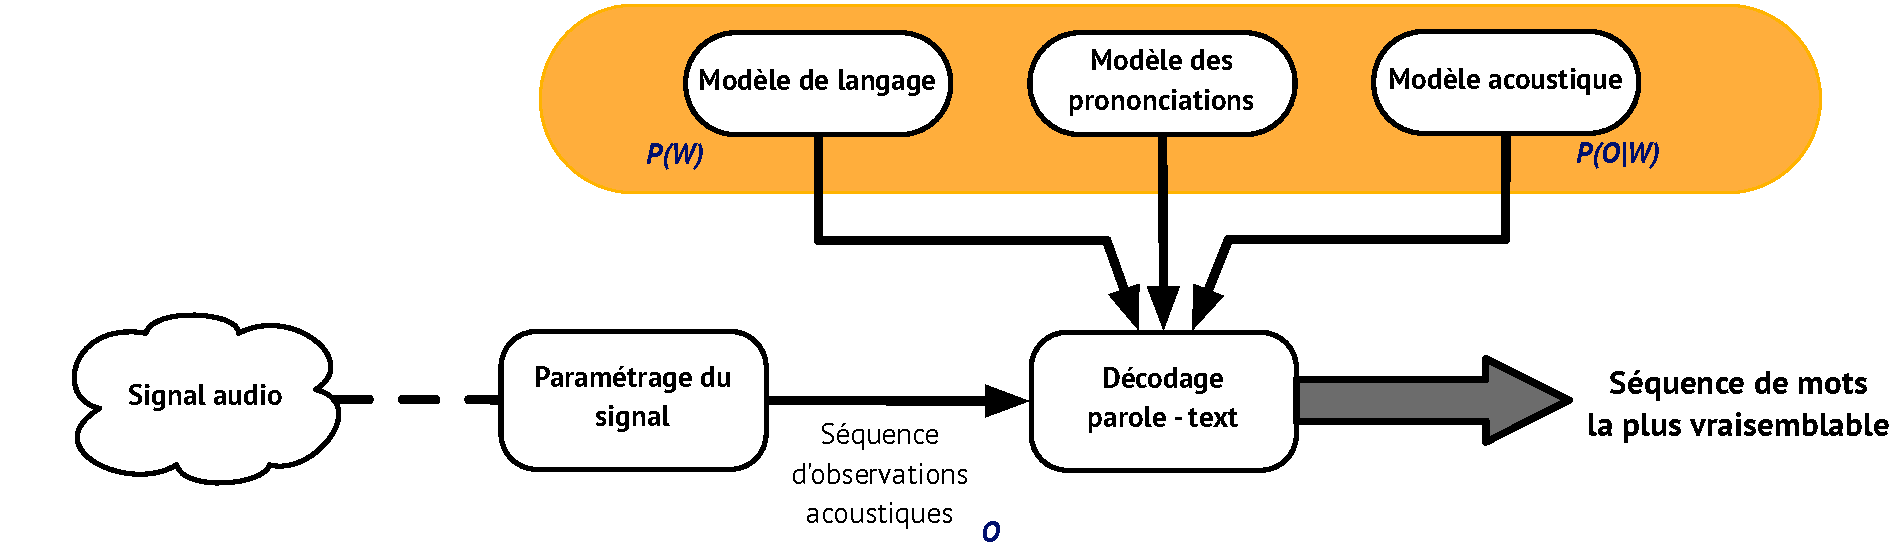
\includegraphics[scale=0.46]{images/pictures/rec_app_v5_c.pdf}
\caption{Architecture d'un système automatique de reconnaissance vocale}
\end{figure}


\minitoc


%=================================================================================
\section{Analyse du signal audio}
\label{AS}
\renewcommand{\rightmark}{Analyse du signal audio}
%=================================================================================

Le signal audio est enregistré avec l'aide d'un ou plusieurs microphones, dont la position et la qualité sont cruciales pour la performance du système de reconnaissance vocal. La présence de plusieurs microphones placés à différents endroits peut servir à localiser le locuteur, à débruiter le signal, à améliorer la performance de reconnaissance,  etc \cite{Kumatani:2012, Swietojanski:2013, Brutti:2014, Wolf:2014, Vincent:2015}.

L'enregistrement d'un signal vocal suit les variations de la pression d'air dans le temps (Fig. \ref{Fig:audioSignal}). 
L'échantillonnage du signal est généralement fait à 16kHz pour une prise de son en direct, et à 8 kHz pour les sons transmis par téléphone.

\begin{figure}[h!]
\begin{center}
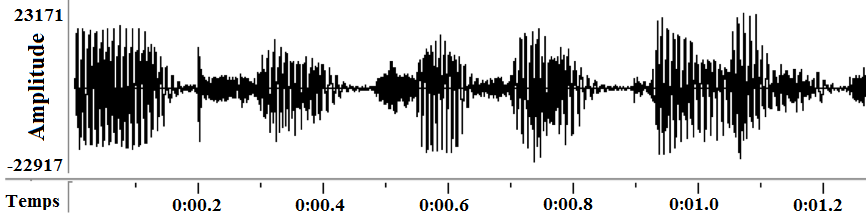
\includegraphics[scale=0.45]{images/pictures/audioSignal.png}
\end{center}
\caption{Exemple d'un signal acoustique \textit{s(t)}}
\label{Fig:audioSignal}
\end{figure}


Le paramétrage du signal est effectué sur des trames successives de signal de courte durée (pour lesquelles  le signal peut être considéré comme étant quasi stationnaire, typiquement 25 ms). Les trames successives se recouvrent et le décalage entre deux trames successives est typiquement de 10 ms \cite{Picone:1993}. 
Un ensemble des paramètres acoustiques est extrait sur chaque trame. 
Cette extraction a pour but de sélectionner les paramètres les plus importants de la parole, tout en réduisant la dimensionnalité des données. 

%%%%%%%%%%%%%%%%%%%%%%%%%%%%%%%%%%%%%%%%%%%%%%%%
\hiddensubsection{Analyse MFCC}

L'analyse acoustique \acrshort{MFCC} (\textit{Mel Frequency Cepstrum Coefficients}) \cite{Davis:1980} (fréquemment utilisée et également utilisée dans nos travaux) implique plusieurs traitements sur le signal audio :\\

\begin{figure}[h]
\begin{center}
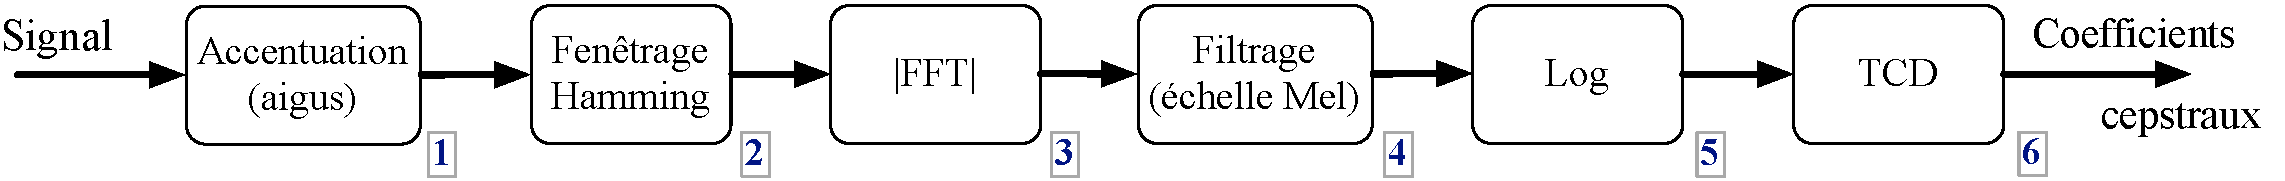
\includegraphics[scale=0.39]{images/pictures/MFCC_v2.pdf}
\end{center}
\caption{Principe de l'analyse cepstrale}
\label{Fig:cepstres}
\end{figure}


\textbf{1)}  La pré-accentuation privilégie les sons aigus (hautes fréquences) :
\begin{equation}
s_{1}(t) = s(t) - 0,98 \cdot s(t - 1)
\end{equation}


\textbf{2)} Le fenêtrage de Hamming permet de réduire les discontinuités dans le signal :

\begin{equation}
h(n)=\left\{\begin{matrix}
0,54 - 0,46 \cdot cos(2\pi \frac{n}{N-1}), si\ 0\leq n \leq N-1 \\ 
0, sinon
\end{matrix}\right.
\end{equation}

\hskip-18pt où $N$ est la taille de la fenêtre. Le signal devient :
\begin{equation}
s_{2}(t) = s_1(t) \cdot h(t)
\end{equation}


\textbf{3)} La transformé de Fourier est appliquée sur chaque trame 

\begin{equation}
S_{3}(f) = \sum\limits_{n=0}^{N-1}s_{2}(n)e^{-i2\frac{\pi}{N}fn}
\end{equation}

\begin{figure}[h!]
\begin{center}
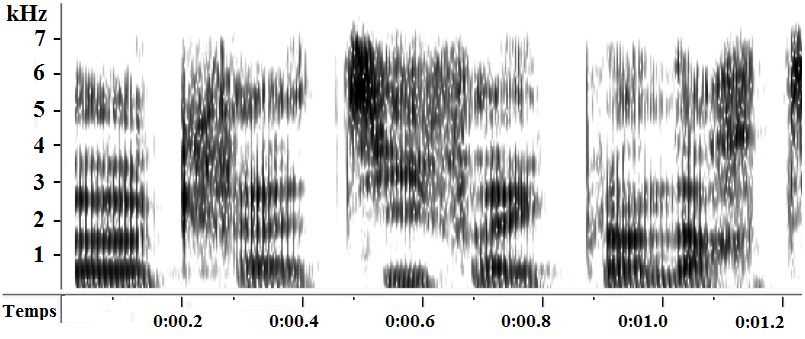
\includegraphics[scale=0.44]{images/pictures/spectrogramme.png}
\end{center}
\caption{Spectrogramme d'un signal audio de parole}
\label{Fig:spectrogramme}
\end{figure}


Cela donne un spectre fréquentiel à court terme. 
Le spectrogramme montre l'évolution temps-fréquence du signal (Fig. \ref{Fig:spectrogramme}); les maxima d'énergie sont indiqués par des zones sombres.


\textbf{4)} Les filtres triangulaires uniformément espacés sur l'échelle Mel (cf. Fig. \ref{Fig:Mel}) réduisent le nombre de bandes de fréquence, par rapport à la FFT (transformée de Fourier) et modélisent la nonlinéarité de la perception audio humaine au niveau des fréquences. 
Chaque filtre fournit un coefficient qui donne l'énergie du signal dans la bande qu'il couvre.

\begin{figure}[h!]
\begin{center}
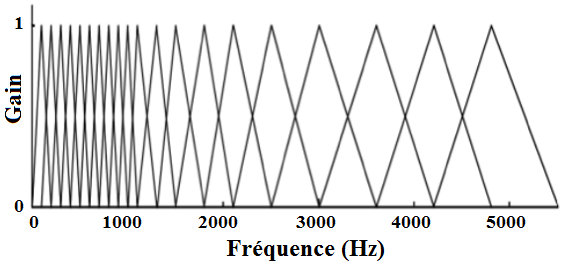
\includegraphics[scale=0.6]{images/pictures/Mel.png}
\end{center}
\caption{Banc de filtres à échelle Mel; répartition linéaire jusqu'à 1000 Hz, logarithmique au delà}
\label{Fig:Mel}
\end{figure}

\textbf{5)} Le passage dans le domaine log-spectral permet de déconvoluer le signal et de le compresser.

\textbf{6)} Un ensemble de $M$ coefficients cepstraux (en général, $M$ choisit entre 10 et 15) sont alors calculés grâce à la transformée en cosinus discrète :

\begin{equation}
c_{i}=\sum\limits_{j=1}^{N_{f}} S(j)\ cos \left (\pi \cdot i \cdot \frac{j - \frac{1}{2}}{N_{f}} \right ) \ pour \ i=\{1,...,M\}
\end{equation}

\hskip-18pt où $N_{f}$ indique le nombre de filtres Mel utilisés,  $M$ indique le nombre de coefficients et $S(j)$ est le logarithme de l'énergie dans le filtre j.


Généralement, seuls les 13 premiers coefficients \acrshort{MFCC} (de $C_0$ à $C_{12}$) sont retenus. 
Parfois le paramètre $C_0$ peut être remplacé par le logarithme de l'énergie de la trame. 
La prise en compte des dérivées temporelles premières et secondes permet d'obtenir une amélioration notable des performances (pour un total de 39 paramètres).



%%%%%%%%%%%%%%%%%%%%%%%%%%%%%%%%%%%%%%%%%%%%%%%%
\hiddensubsection{Autres types d'analyse}

Un type particulier d'analyse cepstrale est l'analyse MFCC Aurora \cite{Sorin:2004}, qui a été développée pour la reconnaissance distribuée dans le cadre d'une normalisation à l'ETSI (\textit{European Telecommunications Standards Institute}). 
Dans un premier temps l'analyse acoustique a été rendue robuste au bruit en y incluant une étape de débruitage \cite{Macho:2002}. 
Les travaux suivants (dans le cadre de l'ETSI) ont porté sur l'introduction du calcul du pitch (nécessaire pour le traitement des langues tonales, et aussi pour reconstruire un signal de parole compréhensible à partir des coefficients acoustiques) \cite{Sorin:2004}.

D'autres types d'analyses acoustiques existent, notamment les paramètres PLP (\textit{perceptual linear predictive}) \cite{Hermansky:1990} ou les paramètres PNCC (\textit{power-\linebreak normalized cepstral coefficients}) \cite{Kim:2012}, ou des techniques qui réduisent la dimensionnalité des vecteurs acoustiques (dans le but de les décorréler) comme la LDA (\textit{linear discriminant analysis}) \cite{Schluter:2001, Zolnay:2005}, la HLDA (\textit{heteroscedastic linear discriminant analysis}) \cite{Kumar:1998}, la NCA (\textit{neighbour component analysis}) \cite{Singh:2007}, la PCA et l'ICA (\textit{principal / independent component analysis}) \cite{Huang:2001}, etc. 
Des réseaux de neurones peuvent également être utilisés dans la phase d'extraction de paramètres pour calculer les paramètres `bottleneck' \cite{Grezl:2007, Yu:2011, Gehring:2013}. 



%=================================================================================
\section{Modèle de langage}
\label{Chap:LM}
\renewcommand{\rightmark}{Modèle de langage}
%=================================================================================

Les modèles de langage statistiques sont des processus qui permettent d'estimer les probabilités des différentes séquences de mots $P(W)=P(w_{1}, w_{2},..., w_{m-1}, w_{m})$. 
Ces modèles servent à `mémoriser' des séquences de mots à partir d'un corpus textuel d'apprentissage. 
 
Dans le contexte de la reconnaissance de la parole, les modèles de langage servent à guider et à contraindre la recherche parmi les hypothèses de mots alternatives.

%%%%%%%%%%%%%%%%%%%%%%%%%%%%%%%%%%%%%%%%%%%%%%%%
\hiddensubsection{Modèles n-grammes}

Les modèles de langage les plus utilisés (et également utilisés dans notre travail) sont des modèles n-grammes. 
Les modèles de langage n-grammes se basent sur l'approximation que la probabilité d'un certain mot $w_k$ dépend seulement de ses $n-1$ mots précédents $P(w_k|$ $w_{k-(n-1)}, w_{k-(n-2)}, ..., w_{k-1})$; leur apprentissage nécessite un grand corpus de texte. 

La probabilité $P(W)$ est décomposée d'abord avec la règle d'enchaînement :

\vskip-3ex
\begin{equation}
\begin{split}
	P(W) &= P(w_{1}, w_{2},..., w_{m-1}, w_{m}) \\
	     &= P(w_{1}) \cdot P(w_{2}|w_{1}) \cdot P(w_{3}|w_{1}, w_{2}) \cdot ... \cdot P(w_{m}|w_{1}, w_{2}, ..., w_{m-1})
\end{split}
\label{Eq:chain}
\end{equation}

\noindent et ensuite avec l'approximation n-gramme, qui limite l'historique à seulement $n-1$ mots :

\begin{equation}
P(w_{m}|w_{1}, w_{2}, ..., w_{m-1}) \cong P(w_{m} | w_{m-(n-1)}, ..., w_{m-1})
\label{Eq:Markov}
\end{equation}

Dans un modèle 3-gramme (1 mot courant, 2 mots pour décrire l'historique) la probabilité $P(W)$ se calcule avec la formule : 

\begin{equation}
P(W) \cong P(w_{1}) \cdot P(w_{2}|w_{1}) \cdot P(w_{3}|w_{1},w_{2}) \cdot ... \cdot P(w_{m}|w_{m-2},w_{m-1})
\label{Eq:Markov2G}
\end{equation}


%%%%%%%%%%%%%%%%%%%%%%%%%%%%%%%%%%%%%%%%%%%%%%%%
\myparagraph{Diverses méthodes d'estimation}

Pour estimer les probabilités des n-grammes, plusieurs approches ont été considérées au fil des années. 

L'estimation du maximum de vraisemblance est basée seulement sur les fréquences d'occurrence des suites de mots. Une grande probabilité est associée aux séquences de mots qui sont fréquentes dans le corpus d'apprentissage, une très faible probabilité - aux séquence de mots peu fréquentes et une probabilité nulle aux événements inconnus. 

\begin{equation}
P(w_{k}|w_{k-2},w_{k-1})=\frac{count(w_{k-2},w_{k-1},w_{k})}{count(w_{k-2},w_{k-1})}
\end{equation}

Les techniques de \textit{smoothing}, \textit{discounting} et \textit{back-off} essaient d'améliorer la capacité de généralisation d'un apprentissage fait sur un corpus textuel. 
Les connaissances apprises sont forcément liées aux corpus et les informations comprises dans ce corpus ne reflètent pas nécessairement la réalité, l'actualité, ni tous les domaines possibles. Si une séquence de mots est peu fréquente ou même absente dans un corpus, ça ne signifie pas forcément qu'elle n'est pas importante. 

La méthode ``\textit{add-$\alpha$ smoothing}'' ajoute ``$\alpha$'' occurrences fictives dans l'équation de l'estimation du maximum de vraisemblance pour augmenter la probabilité des séquences inconnues (absentes dans le corpus d'apprentissage) :

\begin{equation}
P(w_{k}|w_{k-2},w_{k-1})=\frac{count(w_{k-2},w_{k-1},w_{k}) + \alpha}{count(w_{k-2},w_{k-1}) + \alpha V}
\end{equation}

\hskip-18pt où V est la taille du vocabulaire et $0 < \alpha \leq 1$.

Les méthodes ``\textit{intuition smoothing}'' de Good-Turing, Kneser-Ney et Witten-Bell se basent sur l'intuition que les séquences de mots qui ont été vues une seule fois aident à estimer la fréquence d'occurrence des séquences jamais vues. Elles introduisent une nouvelle notation :

$$N_{c} = \text{le nombre des n-grammes vus \textit{c} fois dans le corpus}$$

Par exemple, la méthode Good-Turing \cite{Good:1953} estime la probabilité des séquences inconnues :

\begin{equation}
	P_{GT}(\text{séquence inconnue}) = \frac{N_{1}}{N}
\end{equation}

\hskip-18pt (où $N$ est le nombre total d'occurrences) et réactualise (``\textit{discounting}'') les probabilités des séquences connues :

\begin{equation}
	P_{GT}(\text{n-gramme vu \textit{c} fois})= \frac{N_{c}^{*}}{N}=\frac{\frac{(c+1)N_{c+1}}{N_{c}}}{N}
\end{equation}

Les méthodes de ``\textit{back-off}'' traitent la diversité des événements inconnus, auxquels les méthodes classiques de lissage (\textit{smoothing}) attribuent la même probabilité. 
Pour cela, elles proposent de prendre en compte un historique plus court pour les événements moyennement fréquents. 
La probabilité ``\textit{back-off}'' du modèle devient :

\begin{equation}
\begin{split}
	p_{n}^{BO}&(w_{k}|w_{k-(n-1)},...,w_{k-1}) =\\
	& \left\{	
	\begin{matrix}
	\alpha_{n}(w_{k}|w_{k-(n-1)},...,w_{k-1}) \text{ , si } count_{n}(w_{k-(n-1)},...,w_{k-1}) > 0     \\ 
	d_{n}(w_{k-(n-1)},...,w_{k-1}) \ p_{n-1}^{BO} (w_{k}|w_{k-(n-2)},...,w_{k-1}) \text{ , sinon} 	\\
	\end{matrix}
	\right.
\end{split}
\end{equation}

\noindent où $\alpha_{n}(w_{k}|w_{k-(n-1)},...,w_{k-1})$ est le modèle de prédiction ajusté et $d_{n}(w_{k-(n-1)},...,w_{k-1})$ est la fonction d'actualisation (\textit{discounting function}). 

Dans le cas de modèles trigrammes, les méthodes d'interpolation impliquent la combinaison des 1-grammes, 2-grammes, 3-grammes pour estimer la probabilités des séquences de mots.

L'interpolation conditionnelle sur le contexte :

\begin{equation}
\begin{split}
	\hat{P} (w_{k}|w_{k-2},w_{k-1}) &= \lambda_{w_{k-2},w_{k-1},w_{k}}\ P(w_{k}|w_{k-2},w_{k-1}) \\ 
	& +\lambda_{w_{k-1},w_{k}}\ P(w_{k}|w_{k-1})  \\ 
	& +  \lambda_{w_{k}}\ P(w_{k}) 
\end{split}
\end{equation}

\hskip-18pt associe différents indices de confiance (à travers les valeurs $\lambda$) au différentes probabilités en fonction de leur contexte (historique).


%%%%%%%%%%%%%%%%%%%%%%%%%%%%%%%%%%%%%%%%%%%%%%%%
\myparagraph{Méthode d'estimation la plus utilisée}

En pratique, la méthode la plus utilisée est celle de Chen-Goodman \cite{Chen:1998} qui propose une modification de la méthode de Kneser-Ney \cite{Ney:1995}. 
La méthode Kneser-Ney (cf. l'équation \ref{Eq:KN}) considère que la probabilité d'un unigramme ne doit pas être proportionnelle au nombre d'occurrences des mots, mais au nombre de différents mots qu'il suit (pour éviter d'attribuer une grande probabilité au mots qui sont fréquents mais qui suivent toujours le même mot).

\begin{equation}
\begin{split}
	& P_{KN} \left(w_k|w_{k-(n-1)}^{k-1}\right) = \frac{max\left\{count(w_{k-(n-1)},...,w_{k}) - D,\ 0\right\}}{count(w_{k-(n-1)},...,w_{k-1})}\ + \\
	& \quad \quad \quad \  \frac{D}{count(w_{k-(n-1)},...,w_{k-1})}\ N_{1+}\left(w_{k-(n-1)}^{k-1}\bullet\right)\ P_{KN}\left(w_k|w_{k-(n-2)}^{k-1}\right) 
\end{split}
\label{Eq:KN}
\end{equation}

La notation $N_{1+}\left(w_{k-(n-1)}^{k-1}\bullet\right)$ désigne le nombre de mots uniques qui suivent au moins une fois le contexte $w_{k-(n-1)}^{k-1}$; $n$ indique l'ordre du modèle.

\begin{equation}
N_{1+}\left(w_{k-(n-1)}^{k-1}\bullet\right) = \ |\{w_k : count(w_{k-(n-1)},...,w_{k-1},\ w_k) \geq 1\}|
\label{Eq:N1}
\end{equation}

La valeur $D$ optimale est $D = \ \nicefrac{N_1}{(N_1 + 2N_2)}$.

La méthode Chen-Godman utilise à la place d'un seul paramètre d'actualisation $D$, trois paramètres d'actualisation $D_1$, $D_2$, $D_{3+}$ qui sont appliqués sur les n-grammes avec une, deux et trois occurrences ou plus (cf. l'equation \ref{Eq:CG}). Ils considèrent que l'actualisation moyenne idéale pour les n-grammes vus une ou deux fois est sensiblement différente de l'actualisation moyenne idéale pour les n-grammes avec des fréquences plus élevées.

\begin{equation}
\begin{split}
	P_{CG} \left(w_k|w_{k-(n-1)}^{k-1}\right) = &\ \frac{count(w_{k-(n-1)},..,w_{k}) - D(count(w_{k-(n-1)},..,w_{k}))}{count(w_{k-(n-1)},...,w_{k-1})} \\
	& + \gamma\left(w_{k-(n-1)}^{k-1}\right) P_{CG}\left(w_k|w_{k-(n-2)}^{k-1}\right)
\end{split}
\label{Eq:CG}
\end{equation}

Les variables $D(c)$ et $\gamma\left(w_{k-(n-1)}^{k-1}\right)$ sont définies par : 

\begin{equation*}
\begin{split}
& D(c) =\  \left\{
	\begin{matrix}
	0 									& \text{ if } c = 0 \\
	D_1 =\ 1 - 2\  \nicefrac{N_2}{N_1}\ Y	& \text{ if } c = 1 \\
	D_2 =\ 2 - 3\ \nicefrac{N_3}{N_2}\ Y		& \text{ if } c = 2 \\
	D_{3+} = \ 3 - 4\ \nicefrac{N_4}{N_3}\ Y 	& \text{ if } c \geq 3 \\
	\end{matrix}\right. \\
& \text{où } Y = \   \nicefrac{N_1}{(N_1+2N_2)} 
\end{split}
\label{Eq:CG1}
\end{equation*}

\begin{equation*}
\gamma(w_{k-(n-1)}^{k-1}) = \frac{D_1N_1\left(w_{k-(n-1)}^{k-1}\bullet\right) + D_2N_2\left(w_{k-(n-1)}^{k-1}\bullet\right) + D_{3+}N_{3+}\left(w_{k-(n-1)}^{k-1}\bullet\right)}{count(w_{k-(n-1)},...,w_{k-1})}
\label{Eq:CG2}
\end{equation*}

Les variables $N_1\left(w_{k-(n-1)}^{k-1}\bullet\right)$, $N_2\left(w_{k-(n-1)}^{k-1}\bullet\right)$ et $N_{3+}\left(w_{k-(n-1)}^{k-1}\bullet\right)$ sont définies de manière analogue à l'équation \ref{Eq:N1}.


%%%%%%%%%%%%%%%%%%%%%%%%%%%%%%%%%%%%%%%%%%%%%%%%
\hiddensubsection{Autres modèles}

Une limitation importante des modèles n-grammes surgit du fait que les liens entre les mots dépendent strictement de leur position dans la phrase. 
Une taille $n$ plus grande permet de retrouver un nombre plus important des liens entre les mots, mais nécessite de plus grands corpus pour leur apprentissage. Dans l'état de l'art, la taille optimale d'un modèle n-gramme est égale à 5 (à condition d'avoir une quantité suffisante de données d'apprentissage). 
Dans la pratique, les modèles 3-grammes et 4-grammes sont les plus répandues. 

Les autres techniques de modélisation statistique du langage incluent des modèles de langage basés sur des classes \cite{Goodman:2001}, des modèles n-grammes cache \cite{Jelinek:1991}, des modèles structurés \cite{Chelba:2000}, des modèles basés sur une forêt aléatoire (mélange de plusieurs arbres de décision) \cite{Xu:2007}, des modèles basés sur un réseau de neurones \cite{Bengio:2003, Schwenk:2007, Mikolov:2010, Mikolov:2011_2, Irie:2015, Masumura:2015} ou une combinaison de plusieurs types de modèles \cite{Mikolov:2011_1}. 

Les modèles de langage basés sur un réseau de neurones sont appliqués dans la reconnaissance automatique de la parole (notamment les modèles récurrents) \cite{Mikolov:2011_2} et dans la traduction automatique \cite{Vaswani:2013}, et fournissent des améliorations significatives par rapport aux modèles n-gramme back-off classiques. 

Les modèles de langage basés sur un réseau de neurones récurrent (\textit{recurrent neural network based language model, RNNLM})  utilisent une couche d'entrée, une couche cachée (la couche du contexte) et une couche de sortie. 
La couche d'entrée au temps $t$ contient le vecteur des mots (un vecteur de taille $N$ qui contient $N-1$ valeurs nulles et une seule valeur égale à 1 pour indiquer quel mot est couramment traité dans la liste de $N$ mots du vocabulaire), complété par le vecteur représentant la couche cachée précédente (au temps $t-1$). La couche cachée est une fonction d'activation sigmoïde. 
 Le vocabulaire contient généralement entre 30K mots et 200K mots. 
 La couche cachée contient entre 30 et 500 unités cachés, en fonction de la taille du corpus d'apprentissage. 
 La couche de sortie donne la distribution de probabilités du mot suivant (fonction d'activation \textit{softmax}), basée sur le mot courant et le contexte précédent. 


%%%%%%%%%%%%%%%%%%%%%%%%%%%%%%%%%%%%%%%%%%%%%%%%
\hiddensubsection{Évaluation}

%Un bon modèle de langage attribué une grande probabilité aux séquences de mots correctes (qui ont un sens et qui respectent la syntaxe de la langue). 

La qualité d'un modèle de langage (sa \textit{perplexité}) est évaluée sur un ensemble de phrases d'un corpus de test avec la formule de l'entropie croisée : 

\begin{equation}
	perplexity(W) = 2^{H(W)}= 2 ^ {\frac{1}{n} log_{2} P(W)}
\end{equation}

\hskip-18pt où $n$ indique le nombre de mots dans l'ensemble de phrases $W$ du corpus.
Plus la perplexité est faible, meilleure est la qualité du modèle. 

La métrique du taux d'erreur de mots \acrshort{WER} (voir section \ref{Sec:Eval}) peut également évaluer la qualité d'un modèle de langage dans le contexte de la reconnaissance automatique de la parole. 



%=================================================================================
\section{Modèle de prononciation}
\renewcommand{\rightmark}{Modèle de prononciation}
%=================================================================================

Le lexique d'un système de reconnaissance vocale précise une ou plusieurs prononciations pour chaque mot. 
Pour le français, les prononciations multiples sont en partie dues aux événements de liaison ou de réduction, dans le cadre desquels un locuteur peut prononcer ou pas un certain phonème  dans un certain contexte. 
Les accents et les dialectes peuvent aussi générer diverses variantes de prononciations. 

La liaison implique la prononciation d'un phonème de liaison entre deux mots. 
Pour donner un exemple : les mots ``les oiseaux'' se prononcent séparément  ``\textipa{l} \textipa{e}'' et ``\textipa{w} \textipa{a} \textipa{z} \textipa{o}'' (en notation API), alors qu'ensemble ils se prononcent ``\textipa{l} \textipa{e} \textbf{\textipa{z}} \textipa{w} \textipa{a} \textipa{z} \textipa{o}''. 

La réduction implique l'omission d'un phonème a priori présent dans la prononciation standard d'un mot, comme dans le cas de ``ce'' qui se prononce normalement ``\textipa{c} \textipa{@}'', mais qui peut également être prononcé simplement ``\textipa{c}'' dans le cas d'une prononciation rapide.

Les variantes de prononciation peuvent être obtenues manuellement, avec l'expertise des linguistes, ou automatiquement - avec des convertisseurs graphèmes-phonème basés sur des techniques comme les JMM (\textit{joint-multigram models}) ou les CRF (\textit{conditional random fields}) \cite{Illina:2011, Jouvet:2012}. 
Le graphème est une lettre ou un ensemble de lettres représentant un phonème. 
Les règles de correspondance entre graphèmes et phonèmes sont complexes, irrégulières et spécifiques à chaque langue.
En général, la conversion graphèmes-phonèmes peut être exprimée comme $\tilde{Q} = \underset{Q}{ArgMax} P(Q,G)$, où $G$ est l'orthographe du mot (séquence de graphèmes) et $Q$ est une prononciation candidate.

La méthode JMM \cite{Bisani:2008} applique un modèle de langage sur des couples \{séquence de graphèmes, séquence de phonèmes\}. L'algorithme d'apprentissage vise à déterminer l'ensemble optimal des séquences de graphèmes et de phonèmes ainsi que le modèle de langage associé, de façon incrémentale : un passage initial crée un modèle très simple, ensuite, chaque nouvelle passe d'apprentissage affine le modèle en agrandissant les séquences (si possible).

La méthode CRF \cite{Wang:2011} modélise la distribution des probabilités conditionnelles d'une séquence d'étiquettes (la séquence de phonèmes) étant donnée une séquence d'observation (la séquence de graphèmes). En l'absence d'un corpus de données pré-étiquetées, les modèles \acrshort{HMM} discrets peuvent être utilisés pour aligner les phonèmes avec les lettres.


%=================================================================================
\section{Modèle acoustique}
\renewcommand{\rightmark}{Modèle acoustique}
%=================================================================================

Le modèle acoustique est un modèle statistique qui estime la probabilité qu'un phonème ait généré une certaine séquence de paramètres acoustiques. 
Une grande variété de séquences de paramètres acoustiques sont observées pour chaque phonème en raison de toutes les variations liées à la diversité des locuteurs, à leur âge, leur sexe, leur dialecte, leur état de santé, leur état émotionnel, etc.


%%%%%%%%%%%%%%%%%%%%%%%%%%%%%%%%%%%%%%%%%%%%%%%%
\hiddensubsection{Modèles \acrshort{HMM}}

Dans notre travail, les modèles acoustiques sont basés sur les modèles de Markov cachés (\textit{Hidden Markov Models}, \acrshort{HMM})  qui définissent la répartition temporelle des paramètres acoustiques pour chaque phonème \cite{Rabiner:1989, Picone:1990}. 

Les modèles de Markov d'ordre 1 sont des automates probabilistes à états finis qui se basent sur l'hypothèse que ``le futur ne dépend que de l'état présent''. 
L'état du modèle au temps \textit{t} ne dépend donc que de l'état du modèle au temps ${t-1}$ : $P(q_{t}|q_1,q_2, ...,q_{t-1}) \cong P(q_{t}|q_{t-1})$ où $q_{t}$ est l'état du système au temps $t$. 
À chaque étape temporelle, le modèle évolue suivant la fonction de transition et passe potentiellement dans un nouvel état; l'évolution du système n'est connue qu'à travers des statistiques.

\begin{figure}[h!]
\centering
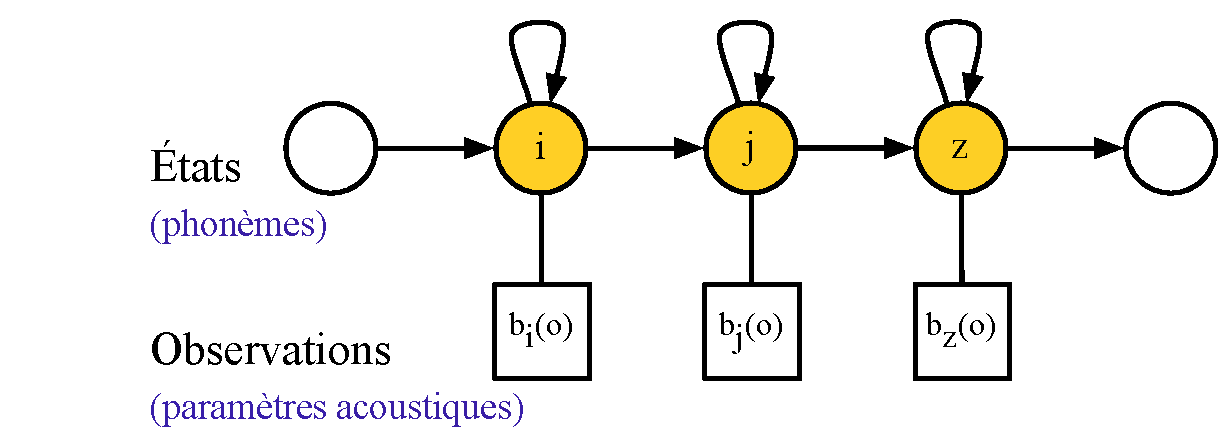
\includegraphics[scale=0.5]{images/pictures/HMM.pdf}
\caption{Exemple de HMM utilisé pour modéliser les phonèmes}
\label{Fig:HMM2}
\end{figure}

Un modèle de Markov caché (\acrshort{HMM}) est un modèle de Markov avec des états non observées (cachés).

Plus formellement, les modèles de Markov cachés sont définis par : 
\begin{itemize}
\item un ensemble fini d'états \{1,...,N\}
\item l'évolution du système $Q=(q_1, ..., q_t, ..., q_T)$ , où $q_t \in \{1,...,N\}$ est l'état du système à l'instant $t$ 
\item la matrice de transitions $A:Q \times Q \rightarrow[0,1]$ où $a_{ij} = P(q_{t} = j | q_{t-1} = i)$, pour les états $i,j \in \{1, ..., N\}$ et $\sum\limits_{j=1}^{N} a_{ij} = 1,\ \forall i$
\item l'ensemble de densités d'observations $B=\{b_j(o_t)\} = P(o_t|q_t=j)$, où $o_t \in \mathbb{R}^{d}$ est le vecteur d'observation à l'instant $t$, et $d$ est la dimension de l'espace des attributs
\item la distribution initiale de probabilités $\pi_{i} = P(q_0=i)$ pour chaque état initial $q_0$
\end{itemize}

En reconnaissance de la parole, les \acrshort{HMM}s sont utilisés pour répondre à la question : ``Ayant un signal acoustique $O$, quel est la phrase ayant la plus grande probabilité d'avoir été prononcée ?''.
Une phrase est composée de mots, les mots sont composés des phonèmes, les phonèmes sont observés à travers des paramètres acoustiques. 
Dans ce contexte~:
\begin{itemize}
\item le signal de parole est produit par une suite d'états; un modèle de Markov est associé à chaque phonème, leur concaténation représentant les mots et les phrases

\item le modèle est stationnaire : $P(q_t = j|q_{t-1} = i) \ = \ P(q_{t+\nu} = j | q_{t+\nu-1} = i)$

\item les observations sont indépendantes : $P(o_t|q_1 ... q_t,o_1 o_2 ... o_{t-1} ) \ = \ P(o_t | q_1 ... q_t)$

\item l'émission d'une observation dépend seulement de l'état courant : $P(o_t|q_t q_{t-1} ... q_1) \ = \ P(o_t | q_t)$

\item la distribution des probabilités d'émission est approchée par un mélange de $k$ lois gaussiennes de la forme :
	$$b_j(o_t) = \sum\limits_{k=1}^{K} \frac{c_{jk}}{\sqrt{(2\pi)^{d} | \Sigma_{jk} |}} exp \left (-\frac{1}{2} (o_t - \mu_{jk})^T \   \Sigma_{jk}^{-1}\ (o_t -\mu_{jk}) \right )$$

où $\mu_{jk}$ et $\Sigma_{jk}$ sont la moyenne et la matrice de covariance de la $k^{ème}$ loi normale de la densité $b_j$, $c_{jk}$ est la pondération de la loi $k$ (avec $\sum\limits_{k=1}^{K}c_{jk} = 1$) et $|\Sigma_{jk}|$ est le déterminant de la matrice $\Sigma_{jk}$.

\end{itemize}

%L'élément le plus important des modèles HMM  est la probabilité d'émission $b_j(o_t)$, qui représente la probabilité d'observer le vecteur de paramètres acoustiques $o_t$ étant  donné l'état du modèle $j$ à l'instant $t$. 

Les modèles \acrshort{HMM} qui utilisent une distribution multi-gaussienne des probabilités d'émission sont couramment qualifiés de \acrshort{HMM}-\acrshort{GMM} dans la littérature \cite{Rabiner:1993}.

\myparagraph{Apprentissage de modèles \acrshort{HMM}-\acrshort{GMM}}

L'apprentissage d'un modèle acoustiques consiste à trouver les meilleures correspondances et le meilleur alignement entre les paramètres acoustiques des signaux audio (chaque intervalle de 10ms du signal audio est associé à un vecteur de paramètres acoustiques) et les transcriptions correspondantes (séquence de mots correspondant à la phrase prononcé). Les frontières entre les mots (et en conséquence entre les phonèmes composants les mots) ne sont pas connues à l'avance. 

L'algorithme de Baum-Welch, basé sur la technique de l'estimation du maximum de vraisemblance, améliore itérativement la solution et garantit de trouver les valeurs optimales des paramètres (optimum local) \cite{Baum:1966}. 
À partir d'un modèle initial $\Lambda_0$ et d'une observation $O$, un nouveau modèle $\Lambda'$ est généré, qui améliore la vraisemblance des données d'apprentissage.  
Le processus se répète en considérant le nouveau modèle obtenu comme modèle initial, jusqu'à la validation de la condition d'arrêt (atteinte d'un optimum ou nombre maximum d'itérations). 

L'algorithme utilise deux variables $\gamma_t(i)$ et $\xi_t(i,j)$ :
\begin{itemize}

\item la probabilité d'être dans l'état $i$ au temps $t$ 
		$$\gamma_t(i) =\ P(q_t=i|O, \Lambda) =\ \frac{\alpha_t(i)\beta_{t}(i)}{\sum\limits_{i=1}^{N}\alpha_t(i)\beta_{t}(i)}$$

\item la probabilité d'être dans l'état $i$ au temps $t$ et dans l'état $j$ au temps $t+1$

\begin{equation*}
\begin{split}
		\xi_t(i,j) =\  & P(q_t=i, q_{t+1}=j|O, \Lambda) \\
			   =\  & \frac{\alpha_t(i)a_{ij}b_j(o_{t+1})\beta_{t+1}(j)}{\sum\limits_{i=1}^{N}\sum\limits_{j=1}^{N}\alpha_t(i)a_{ij}b_j(o_{t+1})\beta_{t+1}(j)}
\end{split}
\end{equation*}

\end{itemize}


La variable $\alpha_t(i) = P(o_1...o_t, q_t=i|\Lambda)$ (variable ``forward'') indique la probabilité d'émettre les $t$ premières observations et d'être à l'état $i$ à l'instant $t$. 
Pour la calculer :
\begin{itemize}
\item initialisation $\alpha_1(i)=\pi_ib_i(o_1)$	
\item induction $\alpha_{t+1}(j)=\left [  \sum\limits_{i=1}^{N} \alpha_t(i) a_{ij}\right ] b_j(o_{t+1}) \text{ où } 1 \leq i \leq N,\ t=1,...,T-1$	
\item terminaison $P(O|\Lambda) = \sum\limits_{i=1}^{N}\alpha_T(i)$
\end{itemize}
	

La variable $\beta_t(j)= P(o_{t+1}...o_{T}|q_t=j, \Lambda)$ (variable ``backward'') indique la probabilité d'émettre les observations de $t+1$ à $T$ en partant de l'état $j$ à l'instant $t$. Pour la calculer :
\begin{itemize}
\item initialisation $\beta_T(i)=1$	
\item induction $\beta_t(i)= \sum\limits_{j=1}^{N} a_{ij} b_j(o_{t+1}) \beta_{t+1}(j) \text{ où } 1 \leq i \leq N,\ t=T-1,...,1$
\item terminaison $P(O|\Lambda) = \sum\limits_{i=1}^{N}\pi_ib_i(o_1)\beta_1(i)$
\end{itemize}

\vskip2ex

Les lois de mises à jour des paramètres pour le nouveau modèle $\Lambda'=\{\bar{\Pi},\bar{A},\bar{B}\}$ :

\vskip2ex

\begin{itemize}  
\item la distribution initiale de probabilités $\bar{\pi}_i=\gamma_1(i)$
\item la matrice de transitions $\bar{a}_{ij} = \frac{\sum\limits_{t=1}^{T} \xi_t(i,j)}{\sum\limits_{t=1}^{T} \gamma_t(i)}$
\item la moyenne de la gaussienne de l'état $i$ (dans cas monogaussian) : 
	$$\mu_i=\frac{\sum\limits_{t=1}^{T} \gamma_t(i)o_t}{\sum\limits_{t=1}^{T} \gamma_t(i)}$$
\item la covariance de la loi normale de l'état $i$ (dans cas monogaussian) : 
	$${\sum}_i=\frac{\sum\limits_{t=1}^{T} \gamma_t(i)(o_t-\mu_i)(o_t-\mu_i)^T}{\sum\limits_{t=1}^{T} \gamma_t(i)}$$
\end{itemize}

\myparagraph{Détails de modélisation}
\label{Sec:HMM}

Typiquement, chaque phonème de la langue est associé à un modèle \acrshort{HMM}  à 3 états. Dans la pratique, comme les réalisations acoustiques des sons sont fortement influencées par des phénomènes de coarticulation avec les sons voisins, les modèles pour les sons sont définis en contexte. Par exemple le phonème /a/ aura un modèle pour [p]\_a\_[r] (i.e. /a/ précédé de /p/ et suivi de /r/), un modèle pour [b]\_a\_[d], un modèle pour [b]\_a\_[s], etc. 
Comme le nombre total de combinaisons possibles devient très grand, les densités de probabilité multi-gaussiennes sont partagées entre les modèles contextuels. Cela permet d'ajuster le nombre total de paramètres à estimer en fonction des corpus disponibles pour leur estimation et des ressources qui seront disponibles lors de la reconnaissance. Dans les outils Sphinx, ces densités partagées sont qualifiées de ``sénones''.

\begin{figure}[h!]
\centering
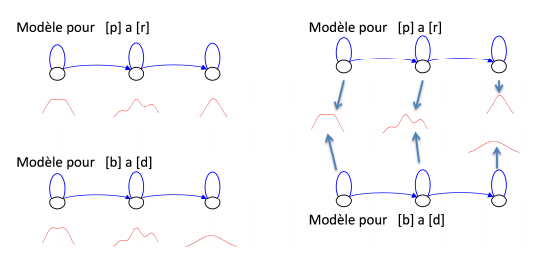
\includegraphics[scale=0.75]{images/pictures/phones-context.png} 
\caption{Principe du partage des densités de probabilité (sénones) entre les états des modèles contextuels des sons (à gauche, pas de partage des densités ; à droite, partage des densités)}
\label{Fig:phones-context}
\end{figure}

Les deux principaux paramètres qui influent sur la taille globale du modèle acoustique (i.e. incluant tous les phonèmes en contexte) sont donc le nombre total de sénones - i.e. le nombre de densités de probabilité partagées entre les modèles contextuels des sons, et le nombre de gaussiennes par densité - un nombre élevé de gaussiennes permet de mieux modéliser les variantes de réalisation acoustique des sons, réalisations qui varient selon les locuteurs (sexe, âge, état de santé, etc), l'environnement (calme, bruité), etc.


%%%%%%%%%%%%%%%%%%%%%%%%%%%%%%%%%%%%%%%%%%%%%%%%
\hiddensubsection{Autres modèles}

Les méthodes les plus récentes de modélisation acoustique proposent des réseaux de neurones profonds dépendants du contexte (\textit{context dependent deep neural network, CD-DNN}) à la place des distributions multi-gaussiennes des probabilités d'émission, et fournissent des améliorations significatives par rapport aux modèles \acrshort{HMM}-\acrshort{GMM} \cite{Dahl:2012, Hinton:2012}. 
Leur succès provient de l'utilisation de plusieurs couches cachées (généralement entre 5 et 7), chacune ayant environ 2048 unités avec un sigmoïde non-linéaire. 
La couche de sortie a une non-linéarité \textit{softmax} et un nombre d'unités de sortie égal au nombre d'états \acrshort{HMM}. 
De plus, l'architecture de calcul utilisant des processeurs graphiques (\textit{GPU}) permet de paralléliser efficacement l'apprentissage et le décodage de la parole. 

Les extensions récentes des modèles DNN incluent les réseaux de neurones convolutifs \cite{Hamid:2012} et les réseaux de neurones récurrents \cite{Sak:2014}.



%.... Direct adaptation of hybrid {DNN/HMM} model for fast speaker adaptation in {LVCSR} based on speaker code \cite{Xue:2014}.


%==============================================================================
\chapter{Processus de reconnaissance}
\renewcommand{\leftmark}{Processus de reconnaissance}
\renewcommand{\rightmark}{}
%==============================================================================

Ce chapitre présente l'algorithme de décodage, les métriques pour évaluer la performance du système et les mesures de confiance.

\minitoc

%%%%%%%%%%%%%%%%%%%%%%%%%%%%%%%%%%%%%%%%%%%%%%%%%%%%%%%%%%%%
\section{Algorithme de décodage}
\renewcommand{\rightmark}{Algorithme de décodage}

Le processus de reconnaissance automatique de la parole (également connu sous le nom de décodage de la parole) détermine la séquence de mots $\hat{W}$ la plus vraisemblable étant donné une séquence d'observations acoustiques \textit{O} :

\begin{equation*} 
	\hat{W}=\underset{W}{ArgMax} P(W|O)= \underset{W}{ArgMax} \frac{P(O|W)P(W)}{P(O)} \cong \underset{W}{ArgMax} P(O|W)P(W)
\label{Eq:Dec}
\end{equation*} 

\noindent où $P(O|W)$ est la probabilité acoustique et  $P(w)$  est la probabilité linguistique.

La formule pour la reconnaissance de la parole suggère que la probabilité du modèle acoustique et la probabilité du modèle de langage peuvent être combinées à travers une simple multiplication. 
En pratique il est nécessaire d'effectuer une pondération. 
Sans cela, la contribution d'un des modèles est négligeable à cause de la différence d'ordre de grandeur de leurs probabilités. 
En effet, les probabilités du modèle acoustique (qui sont en fait les valeurs de densités de probabilité continues multi-gaussiennes) sont beaucoup plus petites que celles du modèle de langage : $P(O|W) \ll P(W)$. 
La solution la plus couramment utilisée pour atténuer ce problème consiste à ajouter un poids, noté $lw$ (\textit{linguistic weight}), au modèle du langage. La nouvelle formule pour la reconnaissance de la parole devient alors :

$$\underset{W}{ArgMax} P(W|O) \cong \underset{W}{ArgMax} P(O|W)P(W)^{lw}$$


Le processus de reconnaissance doit trouver la meilleure séquence d'états (de phonèmes) qui pourrait donner la suite d'observations correspondant à la prononciation d'une certaine phrase (séquence de mots). 
Deux inconnues doivent être gérées dans le cas d'une reconnaissance de parole continue : le nombre de mots que contient la phrase prononcée et les ``frontières'' de chaque mot. 

Les modèles \acrshort{HMM} des mots sont obtenus en concaténant les modèles \acrshort{HMM} des phonèmes (par rapport à leur prononciations définies dans le lexique). 
Les modèles \acrshort{HMM} des séquences de mots sont obtenus en concaténant les modèles \acrshort{HMM} des mots (l'état final d'un mot est concaténé à l'état initial du mot suivant). 
La séquence d'observations acoustiques $O$ est extraite à partir du signal audio (cf. section \ref{AS}).  

Les informations disponibles sont le vocabulaire de $N$ mots, les modèles \acrshort{HMM} des phonèmes : $M_1, M_2, ..., M_p$ et la séquence d'observations acoustiques $O = (o_1, o_2, ..., o_T)$.

La solution optimale, fournie par l'algorithme de Viterbi \cite{Viterbi:1967}, peut être implémentée par une matrice $T \times N$ contenant les valeurs $\delta_t(i)$ qui définissent la vraisemblance du meilleur chemin qui finit à l'état $i$ au temps $t$ :

\begin{equation}
	\delta_t(i) = \underset{q_1,q_2,...,q_{t-1}}{max} P(q_1, q_2, ..., q_t=i, o_1, o_2, ..., o_t | \Lambda)
\end{equation}

\begin{figure}[h!]
\centering
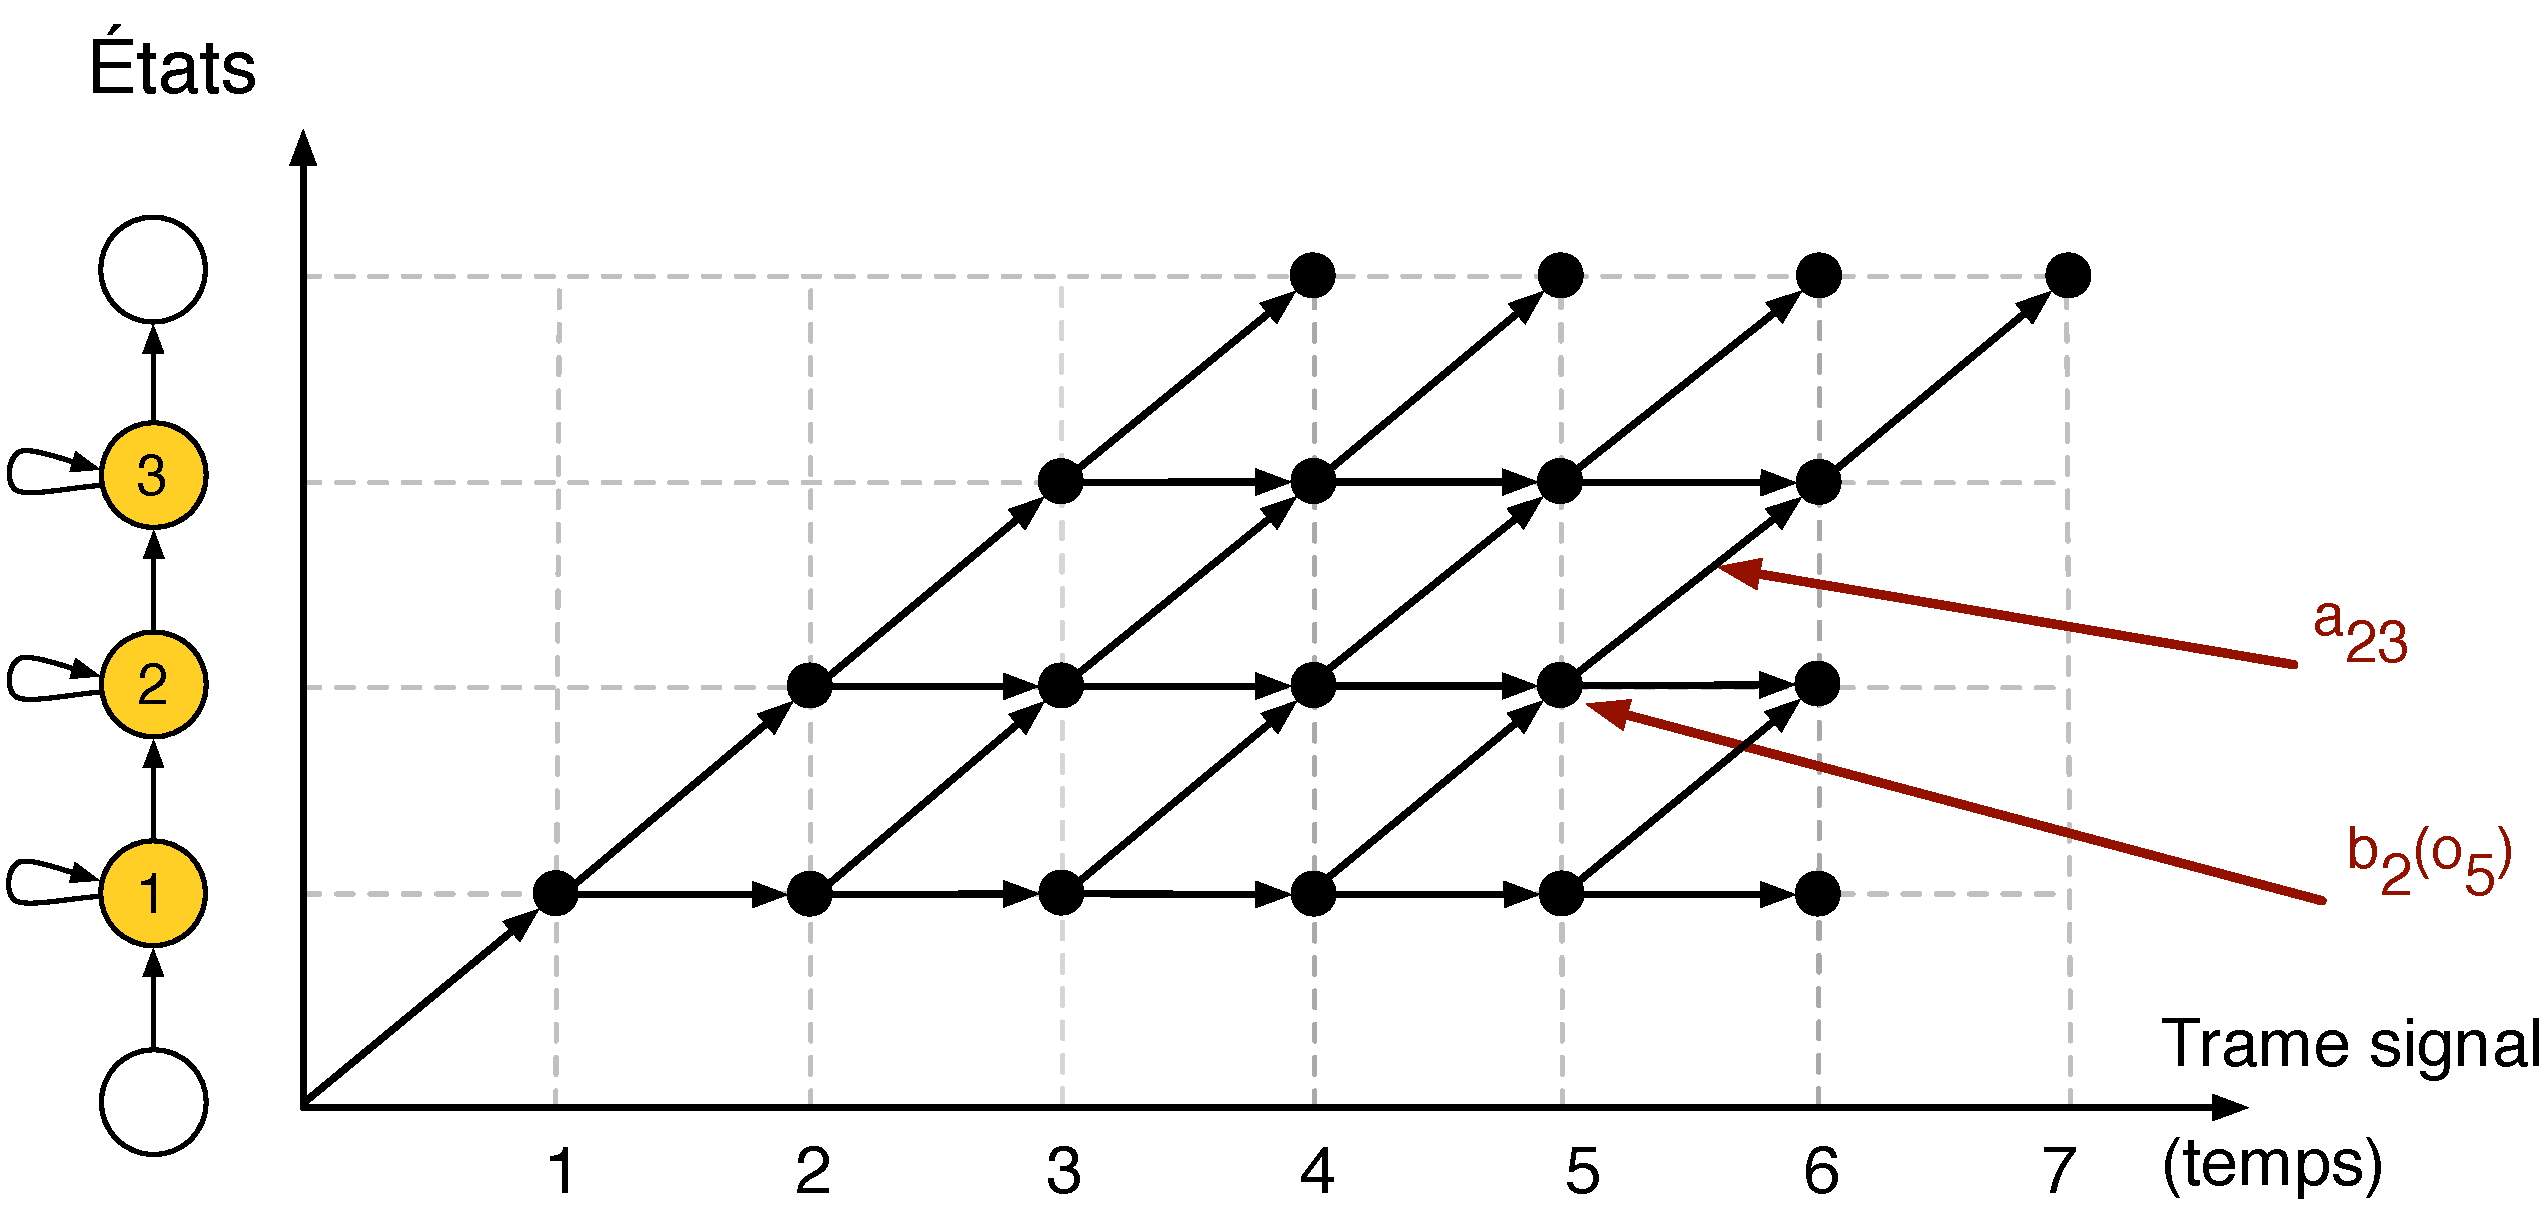
\includegraphics[scale=0.33]{images/pictures/Viterbi.pdf}
\caption{Exemple d'une recherche Viterbi avec un modèle \acrshort{HMM} de 5 états (3 états émetteurs et 2 états non-émetteurs) sur un signal audio de 7 trames (70 milisecondes)}
\label{Fig:Viterbi}
\end{figure}


Le calcul peut être implémenté par récurrence :
\begin{itemize}
\item initialisation : $\delta_{0}^{k}(i) = \pi_{i}^{k}$, avec $k$ désignant l'un des mots du vocabulaire pouvant commencer une phrase (d'après le modèle de langage)
\item hypothèse de récurrence : 	
	\begin{enumerate}
	\item[$\cdot$] état non initial du mot $k$ : \\
			$\delta_{t}^{k}(j) = \underset{i}{max} (\delta_{t-1}^{k}(i) \cdot a_{ij}^{k}) \cdot b_{j}^{k}(o_t)$		
	\item[$\cdot$] état initial du mot $k$ :	\\
			$\ \quad \delta_{t}^{k}(i) = \ max \left (\delta_{t-1}^{k}(i) \cdot a_{ii}^{k},\ \underset{l}{max} \left (\delta_{t-1}^{l}(\text{état final}(l)) * P(w_k|w_l) \right ) \right ) \cdot b_{i}^{k}(o_t)$
	\end{enumerate}	
\item terminaison : $P = \underset{k}{max} (\delta_T^{k}(i))$
\end{itemize}	

Une structure supplémentaire est utilisée pour mémoriser l'état qui a donné le maximum de vraisemblance à chaque pas, afin de retrouver la séquence de mots. 

Le système de reconnaissance fournit généralement la phrase la plus probable (séquence de mots ayant la plus grande vraisemblance $\delta_T$) comme seule et unique solution. 

Cependant, d'autres formes de représentation de résultats de reconnaissance existent, comme la liste de $n$ meilleurs résultats ou le graphe de mots, qui sont générées avec
 plusieurs passes de décodage (une première utilisant des modèles moins précis pour restreindre l'espace de recherche, et les autres avec des modèles plus détaillés pour re-estimer les scores).  
La liste de $n$ meilleurs résultats (\textit{n-best list}) est constituée d'un sous-ensemble de phrases hypothèses générées par le décodeur suivant les meilleurs scores de vraisemblance; la plupart de phrases ne différent entre elles que d'un mot. 
Le graphe de mots mémorise les multiples chemins possibles du début à la fin de la phrase, indexés par rapport au temps (\textit{frame positioned word graph}) ou par rapport à la position de mots dans la phrase  (\textit{word positioned word graph}, autrement connus sous le nom de réseaux de confusion).   

%%%%%%%%%%%%%%%%%%%%%%%%%%%%%%%%%%%%%%%%%%%%%%%%%%%%%%%%%%%%
\section{Évaluation des performances}
\label{Sec:Eval}
\renewcommand{\rightmark}{Évaluation des performances}

L'évaluation de la reconnaissance de la parole est donnée par le critère du taux d'erreur de mots \acrshort{WER} (\textit{Word Error Rate}) qui mesure le rapport du nombre d'erreurs de reconnaissance sur le nombre total de mots prononcés (cf. l'équation \ref{Eq:WER}). Il y a trois types d'erreurs de reconnaissance : substitution (S), omission (O) et insertion (I). 
La vérification des erreurs de reconnaissance nécessite une transcription de référence, qui est généralement créé manuellement. 

\begin{equation}
	WER = \frac{S + O + I}{N_{mots}}
\label{Eq:WER}
\end{equation}

Une autre mesure d'évaluation est fournie par le critère du taux d'erreur de phonèmes \acrshort{PER} (\textit{Phoneme Error Rate}), mesuré au niveau des phonèmes :

\begin{equation}
	PER = \frac{S + O + I}{N_{\text{phonèmes}}}
\label{Eq:PER}
\end{equation}

Dans l'exemple donné dans le tableau \ref{Tab:WER}, le système de reconnaissance a fait 3 erreurs~: 1 omission (du mot `qui') et 2 substitutions (de mots `a' et `été'). Le taux d'erreur de mots est de $3/8=37.50\%$.

\begin{table}[h!]
\centering
\begin{tabular}{|lcccccccc|}
\hline
Référence :	& c' & est & son & bureau & \textbf{\color{darkgreen}qui} & \textbf{\color{blue}a}  & \textbf{\color{blue}été}   & perquisitionné	\\
Hypothèse :	& c' & est & son & bureau & 				  & \textbf{\color{blue}c'} & \textbf{\color{blue}était} & perquisitionné	\\ \hline
Évaluation :	&    &	   & 	 & 	  & \textbf{\color{darkgreen}O}   & \textbf{\color{blue}S}  & \textbf{\color{blue}S}	 &			\\ \hline
\end{tabular}
\caption{Évaluation d'un résultat du décodage}
\label{Tab:WER}
\end{table}

La comparaison entre deux séquences (de mots) $A=a_1,a_2,...,a_m$ et $B=b_1,b_2,...,b_n$ est effectuée avec l'algorithme ``edit distance'' de programmation dynamique de Wagner–Fischer \cite{Wagner:1974}, qui calcule le coût minimum de mise en correspondance.

\begin{table}[h!]
\centering
\begin{tabular}{|rl|}
\hline
Référence :	& c' est son bureau qui a été perquisitionné 						\\
Hypothèse :	& c' est son bureau c' était perquisitionné 						\\ \hline
Solution1 :	& {\color{darkgreen} omission}(qui) + {\color{blue}substitution}(a $\rightarrow $c') + {\color{blue}substitution}(été $\rightarrow$ était)	\\
Solution2 :	& {\color{blue}substitution}(qui $\rightarrow$ c') + {\color{darkgreen} omission}(a) + {\color{blue}substitution}(été $\rightarrow$ était)	\\
Solution3 :	& {\color{blue}substitution}(qui $\rightarrow$ c') + {\color{blue}substitution}(a $\rightarrow$ était) + {\color{darkgreen} omission}(été)	\\
\hline
\end{tabular}
\caption{Solutions multiples pour la mise en correspondance d'une hypothèse de reconnaissance avec la transcription de référence}
\label{Table:MS}
\end{table}

Plusieurs chemins peuvent avoir le même coût minimum (cf. le tableau \ref{Table:MS}). 
C'est seulement ce coût qui établit la performance de reconnaissance. 


%===================================================================================
\section{Mesures de confiance}
\renewcommand{\rightmark}{Mesures de confiance}
%===================================================================================

L'algorithme de décodage est un processus probabiliste qui recherche la meilleure adéquation entre un signal audio et une séquence de mots. Cependant, cette adéquation risque de contenir des erreurs de reconnaissance même dans les meilleures conditions d'application. Ces erreurs de reconnaissance peuvent être liées au modèle de langage (le plus souvent à cause des mots hors-vocabulaire), au modèle de prononciation (prononciation non-définie pour un mot connu) ou au modèle acoustique (bruits inconnus, locuteurs trop différents). L'algorithme de reconnaissance affiche simplement le message décodé, mais il ne peut pas dire de lui même (de manière certaine) si le message contient des erreurs, ni où se trouvent ces erreurs. 

Sachant que les systèmes de reconnaissance font assez souvent des erreurs, les chercheurs ont introduit diverses mesures pour donner une indication de la pertinence de la reconnaissance, connues sous le nom des ``mesures de confiance'' \cite{Jiang:2005, Razik:2007}. 
Ces mesures sont calculées soit sur les unités reconnues (mots, phonèmes, ...), soit sur les phrases entières, en fonction de l'objectif de l'application. 
Les trois types de mesures de confiance les plus courantes sont celles fondées sur une combinaison des paramètres prédictifs \cite{Wessel:1999, Zhang:2001}, sur le rapport de vraisemblance \cite{Rose:1995, Weintraub:1997} ou sur la probabilité a posteriori \cite{Rueber:1997, Kemp:1997, Wessel:2001}. 

Les sources d'information utilisées pour la conception des paramètres prédictifs incluent les informations issus du décodage : les scores acoustiques par trame, les scores du modèle de langage, l'occurrence des mots parmi les $N$ meilleures hypothèses, l'occurrence des mots parmi les hypothèses obtenues en variant le poids du modèle de langage, le nombre de solutions alternatives par arc dans le graphe de mots, etc. 

Les mesures fondées sur le rapport de vraisemblance utilisent deux hypothèses : H0 - le message est correctement reconnu et son modèle acoustique associé est le correct, H1 - le message n'est pas correctement reconnu et son modèle acoustique associé n'est pas le bon. Les hypothèses alternatives peuvent être obtenues avec l'aide des ``anti-modèles'' (appris sur des alignement incorrects, e.g. erreurs de reconnaissance sur un ensemble d'apprentissage).  

Les mesures de confiance a posteriori des mots sont calculés avec la formule :
$$P(w|O)= \frac{P(O|w)P(w)}{P(O)} \cong \frac{P(O|w)P(w)}{\sum\limits_{w'} P(O|w')P(w')}$$

La probabilité $P(w|O)$ désigne une bonne mesure de confiance, à condition que le produit entre la probabilité du modèle acoustique $P(O|w)$ et la probabilité du modèle de langage $P(w)$ soit bien normalisée par la probabilité acoustique $P(O)$. 
Le calcul de la probabilité acoustique $P(O)$ doit tenir compte de toutes les hypothèses (de mots / phonèmes / bruits / ...) possibles pouvant générer la séquence de paramètres acoustiques $O$, ce qui est impossible dans la pratique. 
Comme solutions alternatives pour calculer la probabilité acoustique, des chercheurs ont proposé une reconnaissance purement phonétique (avec un modèle acoustique, un modèle de langage et un lexique à base de phonèmes), ou l'utilisation de graphes de mots ou de la liste de $N$ meilleures hypothèses (générés par le décodeur comme solutions alternatives), etc. 

%La probabilité a posteriori d'un mot peut être calculé à partir de la liste de $N$ meilleures phrases ou sur le graphe de mots. 
La mesure de confiance d'un mot calculée sur la liste de $N$ meilleurs résultats est basée sur l'estimation de la probabilité $P(O)$ et sur la  normalisation des probabilités a posteriori de toutes les phrases hypothèses contenant le mot recherché (dans la même position dans la phrase) par rapport à toutes les phrases hypothèses \cite{Weintraub:1997}. 
La mesure de confiance d'un mot calculée sur le graphe de mots utilise les probabilités acoustiques et linguistiques des mots présents dans le graphe de mots avec l'algorithme \textit{forward-backward} de \cite{Wessel:2001} (qui tient compte des instants début et fin de chaque mot). 

Les mesures de confiance a posteriori apprises sur les graphes de mots offrent généralement la meilleure performance \cite{Jiang:2005}.  

%Concernant l'apport des mesures de confiance dans l'emploi de transcriptions automatiques de parole pour aider la communication avec des personnes sourdes, des tests subjectifs ont montré une préférence pour l'affichage sous forme phonétique pour les mots avec une faible mesure de confiance \cite{Razik:2008}. 



%=================================================================================
\chapter{Conclusions}
\renewcommand{\leftmark}{Conclusions}
\renewcommand{\rightmark}{}
%=================================================================================

Cette partie a débuté avec une présentation de l'évolution des systèmes de reconnaissance de la parole et de quelques uns de leur domaines d'application. 
Partant de la simple reconnaissance de 10 chiffres prononcés par un locuteur connu, la reconnaissance de la parole a beaucoup évolué et peut désormais reconnaître des milliers de mots prononcés par différents locuteurs et dans différentes environnements. 
Cependant, sa performance n'est toujours pas parfaite. Les systèmes actuels ne peuvent pas \underline{tout} reconnaître (toutes les langues, tous les dialectes, toutes les personnes, toutes les variations de la parole liées aux sexe, âge ou maladie, tous les bruits, tous les mots, tous les noms, ...). 
C'est pour cette raison que les applications courantes essayent de répondre à une seule problématique à la fois, en optimisant le système pour l'application visée.  
Les différentes aides étudiées pour les personnes sourdes ou malentendantes comprennent des travaux sur la reconnaissance de traits phonétiques pour aider la lecture labiale, la traduction son - langage des signes grâce à un avatar et l'affichage des sous-titres. Mais à l'heure actuelle il n'y a toujours pas de vraie solution pour eux. 

Ensuite nous avons présenté le fonctionnement d'un système automatique de reconnaissance de la parole, en donnant plus des détails sur les techniques utilisées dans nos expériences (analyse acoustiques MFCC, modèles de langage n-grammes, modèles acoustiques \acrshort{HMM}-\acrshort{GMM}) et en mentionnant des autres techniques, notamment les techniques actuelles (à base de réseaux de neurones). 

Plus brièvement, nous avons rappelé l'algorithme de décodage de la parole qui fournit la phrase la plus probable ayant été prononcée, et les métriques utilisés pour l'évaluation des hypothèses fournies pas le décodeur. 
Enfin, nous avons mentionné différentes techniques de calcul des mesures de confiances utilisées pour évaluer la pertinence du message décodé. 




\stopcontents[parts]
\end{part}



\renewcommand{\leftmark}{}
\renewcommand{\rightmark}{}

%%%%%%%%%%%%%%%%%%%%%%%%%%%%%%%%%%%%%%%%%%%%%%%%%%%%%%%%%%%%%%%%%%%%%%%%%%%%
\begin{part}{Modélisation lexicale}
%%%%%%%%%%%%%%%%%%%%%%%%%%%%%%%%%%%%%%%%%%%%%%%%%%%%%%%%%%%%%%%%%%%%%%%%%%%%


%%%%%%%%%%%%%%%%%%%%%%%%%%%%%%%%%%%%%%%%%%%%%%%%%%%%%%%%%%%%%%%%%%%%%%%%%%%%
\chapter{État de l'art}
\renewcommand{\leftmark}{État de l'art}
\renewcommand{\rightmark}{}
%%%%%%%%%%%%%%%%%%%%%%%%%%%%%%%%%%%%%%%%%%%%%%%%%%%%%%%%%%%%%%%%%%%%%%%%%%%%

%de l'étude a eu comme objectif principal l'extraction d'informations linguistiques pertinentes à partir du signal de parole, en vue de leur affichage sur un terminal pour faciliter la communication avec une personne sourde ou malentendante.

Le premier défi du projet porte sur l'optimisation de la modélisation pour l'extraction d'informations lexicales. 
Nous nous intéressons à l'optimisation des heuristiques de décodage et du choix des unités lexicales (pour définir le lexique et le modèle de langage associé), en vue de faire face aux problématiques liées à la taille de modèles et à la diversité et à l'évolution de domaines d'application. 

Ce chapitre présente l'état de l'art relatif au choix des unités lexicales pour le modèle de langage (considérées seules ou combinées) et à la possibilité d'ajuster le modèle de langage pour pouvoir reconnaitre des mots a priori inconnus.  
Nos travaux sont ensuite positionnés par rapport aux objectifs du projet et à l'état de l'art. 

\minitoc

%===================================================================================
\section{Décodage phonétique}
\renewcommand{\rightmark}{Décodage phonétique}
%===================================================================================

En complément de la section \ref{Chap:LM} qui traite les différentes types de modèles de langage et les différentes méthodes d'estimation de probabilités entre les mots du vocabulaire, cette section s'intéresse aux différentes unités lexicales sur lesquelles un modèle de langage peut être appris.

Les modèles de langage phonétiques sont rarement utilisés pour la reconnaissance de la parole. 
Les liens entre les diverses unités phonétiques sont difficiles à modéliser avec un lexique si limité (moins de 40 phonèmes pour la langue française), peu importe la taille du corpus d'apprentissage. 
De plus, un affichage complet en phonèmes est dur à interpréter sans aucun indice sur les frontières des mots. 
Ils peuvent néanmoins être utilisés avec d'autres objectifs : pour identifier la langue d'une phrase \cite{Yan:1995}, pour identifier le locuteur \cite{Jin:2002}, pour détecter les mots hors-vocabulaire \cite{Szoke:2008}, etc.

La syllabe a été étudiée en tant qu'unité acoustique - pour la reconnaissance de la parole continue avec un grand vocabulaire \cite{Danon:1989, Wu:1998, Zhang:2002, Tachbelie:2012}, généralement en combinaison avec des phonèmes dépendants du contexte \cite{Ganapathiraju:2001, Hamalainen:2005} ou en tant qu'unité acoustique et lexicale \cite{Blouch:2006}. 
Dans \cite{Wu:1998}, la syllabe a été décrite comme une unité attrayante pour la reconnaissance grâce à sa plus grande stabilité, à son lien naturel entre l'acoustique et l'accès lexical et à sa capacité d'intégrer les informations prosodiques dans la reconnaissance. 
Dans \cite{Blouch:2006}, la coarticulation a été modélisée entre les phonèmes à l'intérieur de la syllabe, mais aucune modélisation dépendante du contexte n'a été prise en compte entre les syllabes, de plus le modèle de langage appliqué au niveau de la syllabe était un bigramme.
Pour obtenir les syllabes, plusieurs approches peuvent être considérées : des heuristiques de découpage des chaînes de phonèmes \cite{Blouch:2006}, le principe de la sonorité \cite{Bartlett:2009}, des règles de syllabation \cite{Bigi:2010}, etc. 

Les modèles de langage à base de morphèmes (la plus petite composante linguistique d'un mot qui a un sens) sont utilisés avec succès pour la reconnaissance de la parole amharique, polonaise ou allemande (langues morphologiquement riches) \cite{Tachbelie:2014, Shaik:2011_1, Mousa:2011}. 

Les modèles de langage basés sur les mots (aussi appelés des modèles grand vocabulaire) sont les plus performants et les plus utilisés \cite{Merialdo:1987, Danon:1989, Young:1996}. 
Avoir une quantité importante de mots dans le vocabulaire et dans le modèle de langage favorise la bonne reconnaissance de ceux-ci. 

Cependant, tous les modèles de langage ont une limite; ils sont incapable de reconnaître les mots qui n'appartiennent pas à leur vocabulaire (mots hors-vocabulaire). 
Compte tenu de la quantité limitée des données d'apprentissage, et aussi de la capacité mémoire et de la puissance de calcul limitées des systèmes de traitement (en particulier, pour des systèmes intégrés dans un dispositif portable), il est impossible de concevoir un système de reconnaissance qui couvre tous les mots, et encore moins tous les noms propres et toutes les abréviations. 

%===================================================================================
\section{Modèles hybrides}
\renewcommand{\rightmark}{Modèles hybrides}
%===================================================================================

Une solution pour diminuer les erreurs liées aux mots hors vocabulaire vise à étendre les lexiques de mots avec des fragments de mots.

La méthode proposée dans \cite{Yazgan:2004} utilise un modèle de langage hybride anglais qui combine des mots avec des unités de sous-mots, tels que les phonèmes ou les syllabes, dans le but de détecter les mots hors-vocabulaire. 
Leur modèle de langage hybride est appris sur un corpus combinant les deux types d'unités : les $N$ mots les plus fréquents sont conservés tels quels, et les mots moins fréquents sont décomposés en phonèmes ou en syllabes. 
La séquence correspondante de phonèmes représente la prononciation du mot (par rapport aux variantes de prononciation définies dans le lexique). La séquence de syllabes est construite sur la séquence de phonèmes en suivant le principe de l'attaque maximale (\textit{maximum onset principle}). 
Trois vocabulaires différents sont évalués : parmi les 5K mots les plus fréquents, les premiers 2K mots sont conservés tels quels, et les autres sont décomposés en phonèmes ou en syllabes; idem pour les vocabulaires de 10K et 20K mots les plus fréquents, les 5K premiers mots sont conservés tels quels, et les autres sont décomposés en phonèmes ou en syllabes. 
Une étude pour récupérer la bonne identité (orthographe des mots) avec la bonne prononciation des mots hors-vocabulaire est effectuée, mais seule une petite quantité de mots hors-vocabulaire est correctement trouvée. 

Les vocabulaires ouverts ont été également étudiés dans \cite{Bisani:2005}, où les mots et des fragments de mots sont mélangés conjointement dans un modèle de langage hybride (anglais). 
Les fragments de mots sont des ``graphones'' $q=\left(g,\varphi\right)$, c'est-à-dire des ensembles d'une séquences de lettres $g$ et une séquences de phonèmes $\varphi$ (séquences ayant des longueurs éventuellement différentes). 
Trois vocabulaires différents sont évalués : les 5K mots les plus fréquents, les 20K mots les plus fréquents et les 64K mots les plus fréquents. Les modèles graphème-phonème sont appris séparément pour chaque vocabulaire avec un modèle trigramme, en utilisant des séquences de lettres et de phonèmes de longueurs variables (entre 2 et 6). Les graphones obtenus avec cette méthode sont ensuite ajoutés au vocabulaire : entre 1K et 4K graphones pour le vocabulaire de 5K mots, entre 1K et 15K graphones pour le vocabulaire de 20K mots, et entre 3K et 29K graphones pour le vocabulaire de 64K mots. Le modèle de langage hybride est appris sur un corpus combinant les deux types d'unités :  les $N$ mots les plus fréquents sont conservés tels quels, tous les autres mots étant remplacés par la séquence de graphones la plus probable. 
Une analyse de l'impact des mots hors-vocabulaire sur le taux d'erreur de reconnaissance de mots est effectuée, en utilisant les différents lexiques. Les résultats obtenus avec les modèles hybrides surpassent ceux des modèles classiques (basés uniquement sur des mots) : l'amélioration est plus importante quand il y a une grande quantité de mots hors-vocabulaire. 

Dans \cite{Rastrow:2009_1}, les unités de sous-mots correspondent à des séquences de phonèmes de longueurs variables, déterminées automatiquement à partir de données (anglaises). 
Six vocabulaires différents sont évalués, en choisissant les \{10K, 20K, 30K, 40K, 60K ou 84K\} mots les plus fréquents. 
Le corpus d'apprentissage est converti en phonèmes en utilisant le lexique de prononciations associé à chaque vocabulaire (les mots hors-vocabulaire sont donc exclus).  
Ce corpus est utilisé pour apprendre un modèle de langage phonétique 5-gramme, qui va ensuite fournir les séquences de phonèmes de longueur variable (jusqu'à 5). 
Le modèle de langage hybride est appris sur un corpus combinant les deux types d'unités :  les $N$ mots les plus fréquents sont conservés tels quels, tous les autres mots étant remplacés par une suite des fragments (séquences de phonèmes). 
L'algorithme de recherche commence par affecter le fragment le plus long possible et continue de manière itérative à ajouter le plus long fragment suivant, jusqu'à ce que la prononciation complète du mot soit représentée par des unités de sous-mots (les séquences de phonèmes utilisées appartiennent au modèle de langage phonétique 5-gramme associé au lexique courant). 
Un ensemble de 20K fragments (séquences de phonèmes) est ajouté à tous les vocabulaires hybrides. 
Une telle extension fournit de meilleures correspondances acoustiques sur les parties hors-vocabulaire du signal de parole (comparé au modèles basés uniquement sur des mots), ce qui réduit le taux d'erreur phonétique. 
De plus, les régions des mots hors-vocabulaire sont détectées en utilisant la probabilité postérieure des unités de sous-mots à l'intérieur des réseaux de confusion obtenus avec le modèle hybride \cite{Rastrow:2009_2}. 

Des études plus récentes \cite{Shaik:2011_2} ont examiné la combinaison de plus de deux types d'unités lexicales (allemandes) dans le même vocabulaire et modèle de langage : des mots, des morphèmes (la plus petite composante linguistique d'un mot qui a un sens) ou des syllabes, et des graphones à base de morphèmes (un ensemble considérant une séquence de morphèmes avec une séquence de phonèmes) ou des graphones à base de syllabes (un ensemble considérant une séquence de syllabes avec une séquence de phonèmes). 
Deux lexiques considérant les trois unités lexicales sont évalués : le premier combinant 5K mots, 95K morphèmes et 200K graphones à base de morphèmes, et le deuxième - 10K mots, 90K syllabes et 200K graphones à base de syllabes.  
Le modèle de décomposition en morphèmes est appris avec l'outil \textit{Morfessor} qui utilise le principe de la longueur de description minimale (\textit{minimum description length, MDL}), sur une liste de mots ayant une fréquence d'au moins 5 occurrences.  
Les mots sont décomposés en syllabes avec l'outil \textit{KombiKor} utilisant des règles phonologiques. 
Chaque modèle graphème-phonème est appris avec un modèle 3-gramme, en utilisant une longueur optimale de la séquence de lettres et de la séquence de phonèmes (qui minimise le taux d'erreur de phonèmes). Pour créer les graphones à base de morphèmes ou de syllabes, la séquence de lettres est convertie en morphèmes ou en syllabes (un alignement lettres-phonèmes permet de récupérer les séquences de phonèmes associées aux morphèmes ou aux syllabes).  
Le modèle de langage hybride est appris sur un corpus combinant les trois types d'unités~: les $N$ mots les plus fréquents sont conservés tels quels, les mots moins fréquents (dans un vocabulaire de 100K mots) sont remplacés par des morphèmes ou par des syllabes; les mots hors-vocabulaire sont remplacés par des ``graphones'' (à base de morphèmes ou de syllabes). 
Les meilleurs résultats sont obtenus avec la combinaison de mots, morphèmes et ``graphones'' à base de morphèmes. 
Pour récupérer facilement les mots à partir des unité des sous-mots, un symbol ``+'' est attaché à la fin de chaque unité de sous-mots non-finale. Ainsi, environ 40\% de mots hors-vocabulaire sont correctement identifiés. 


%===================================================================================
\section{Ajout de nouveaux mots}
\renewcommand{\rightmark}{Ajout de nouveaux mots}
%===================================================================================

D'autres solutions peuvent être envisagées pour reconnaître des mots qui sont inconnus pour le système. 

La solution la plus classique suggère une adaptation du modèle de langage \cite{DeMori:1999, Bellegarda:2004} afin d'apprendre les probabilités des n-grammes associés aux nouveaux mots. 
Les trois techniques principales pour adapter un modèle de langage sont : l'interpolation, l'utilisation de contraintes et l'extraction de méta-données. 
Dans le cas de l'interpolation, un nouveau modèle de langage est appris sur un nouveau corpus (représentant les mots manquants ou un nouveau domaine d'application) et il est ensuite combiné avec le modèle initial.  
La solution de \cite{Liu:2008} propose une interpolation entre plusieurs modèles de langage avec des poids d'interpolation dépendants du contexte, rendant ainsi possible l'adaptation d'un modèle de langage à une tâche particulière. 
Concernant l'utilisation de contraintes, divers paramètres peuvent être extraits à partir du nouveau corpus (un historique de mots, probabilités des 1-grammes, ...) et utilisés pour modifier les probabilités du modèle initial. 
Les informations liées à la thématique, à la sémantique ou à la syntaxe d'un nouveau corpus (méta-données) peuvent aussi servir pour l'adaptation du modèle initial. 
Cependant, le bon fonctionnement des techniques d'adaptation est directement lié à l'utilisation d'une grande quantité de nouvelles données (ces données ne sont pas toujours faciles à trouver).

Les fréquences de 2-grammes inconnus peuvent aussi être estimées sur les données disponibles sur internet \cite{Keller:2003}.

Une autre approche implique l'utilisation des modèles de langage basés sur des classes \cite{Brown:1992, Suhm:1994} : les nouveaux mots sont simplement ajoutés dans une classe. 
Dans le passé, les scientifiques laissaient l'utilisateur choisir la meilleure classe pour le nouveau mot \cite{Asadi:1991}, mais la classe peut aussi être choisie automatiquement, en se basant sur la similarité entre le nouveau mot et les mots de la classe. 
La similarité entre deux mots peut être estimée avec diverses méthodes. 

Dans \cite{Prazak:2007}, les mots sont associés à une classes par rapport à des étiquettes morphologiques (15 symboles représentant diverses informations sur les classes grammaticales, le genre, le nombre, le temps du verbe, le degré de comparaison, négation, etc). Les étiquettes sont attribuées automatiquement par un analyseur morphologique tchèque. Leur modèle contient 112K mots repartis en 1,5K classes (1,5K étiquettes morphologiques uniques). 

L'approche de \cite{Naptali:2012} propose d'utiliser un modèle de langage basé sur des classes, pour lequel chaque mot du vocabulaire fait partie d'une classe singleton; les mots hors-vocabulaire (mais présents dans le corpus d'apprentissage) sont associés à la classe de leurs mots similaires présents dans le vocabulaire (basé sur la mesure du cosinus de la similarité entre les vecteurs représentant les mots), et les autres mots n'ayant pas de données représentatives sont associés à la classe générale <unk>. 
Des documents représentant les mots hors-vocabulaire sont récupérés en ligne (100 pages web pour chaque nouveau mot) et une représentation matricielle de ces documents est conçue pour chaque nouveau mot, par rapport aux mots connus (les 20K mots les plus fréquents) et au nouveau mot courant. 
Deux types de représentations matricielles sont considérés.  
La première matrice $A=(n+1)\times(m)$ contient $n+1$ lignes (les $n$ mots connus les plus fréquents et un seul nouveau mot) et $m$ colonnes (le nombre de documents récupérés en ligne), dont les éléments \{$a_{ij}$\} indiquent la fréquence d'occurrence du mot $w_i$ dans le document $d_j$. 
La deuxième matrice $A=(n+1)\times(n+1)$ contient $n+1$ lignes et $n+1$ colonnes (les $n$ mots connus les plus fréquents et un seul nouveau mot), dont les éléments \{$a_{ij}$\} indiquent le nombre de fois que le mot $w_i$ suit le mot $w_j$. 
Chaque mot $w_k$ (connu ou nouveau) est ensuite représenté par un vecteur $w_k=A^Tc_k$, où $c_k$ est un vecteur discret ayant le $k$ième élément égal à 1 et les autres égaux à 0 (vecteur de dimension $n+1$). 
La similarité entre un nouveau mot et les mots connus est ensuite calculée par le produit entre le cosinus de la similarité entre les vecteurs de mots et l'importance du mot connu dans le corpus d'apprentissage : 
$sim(w_i,w_{{oov}_j})=cos(w_i, w_{{oov}_j}) \ idf(w_i)$. % = \frac{w_i \cdot w_{{oov}_j}}{|w_i||w_{{oov}_j}|} \ log\left(\frac{dimension(w_i)}{\#non-zero\ cells}\right).$
Chaque nouveau mot est associé à la classe de son mot connu le plus similaire $C_{{oov_j}}=$ $C_{{argmax_{w_i \in IV}}} sim(w_i,w_{oov_j})$. 
Leur approche dépasse la performance des modèles baseline, surtout lorsqu'un nouveau mot est associé à plusieurs classes.  

D'autres méthodes permettent d'ajouter de nouveaux mots dans le modèle de langage sans réapprendre le modèle, en utilisant très peu de données associées aux nouveaux mots \cite{Allauzen:2005}, ou même sans données associées aux nouveaux mots \cite{Martins:2008}. 
La méthode proposée dans \cite{Allauzen:2005} utilise un modèle de langage n-gramme basé sur des mots et sur des classes grammaticales, et l'ajout de nouveaux mots se fait sans modifier le modèle de langage baseline.  
Une liste de 20 classes grammaticales \acrshort{POS} (les plus fréquentes, auxquelles sont ajoutés des discriminations singulier / pluriel) est définie à partir d'un sous-corpus du corpus d'apprentissage. 
Par rapport au corpus d'apprentissage complet et au vocabulaire de référence, les mots connus (dans le vocabulaire) sont utilisés tels quels, les mots inconnus (hors-vocabulaire) ayant une classe grammaticale fréquente (dans la liste de 20 classes sélectionnées) sont remplacés par leurs étiquettes \acrshort{POS}, et les autres mots inconnus sont remplacés par l'étiquette générale <unk>. 
Une liste de nouveaux mots (qui ne sont pas connus par le système, mais qui doivent être reconnus) est définie à partir des méta-données associées aux fichiers audio, qui incluent la date et l'heure de l'enregistrement, des détails techniques, les noms des locuteurs et un résumé de l'émission. 
Cette liste comprend principalement des noms propres, des verbes conjugués est des substantifs. 
Le résumé est utilisé pour récupérer les classes grammaticales \acrshort{POS} de nouveaux mots. 
Les nouveaux mots sont ensuite inclus dans le vocabulaire en tant que membres de leurs classes grammaticales. 
La probabilité d'un nouveau mot $w$ étant donné un historique $h$ est calculée par $P(w|h)=P(c_w|h)P(w|c_w)$, où $c_w$ représente la classe grammaticale du mot $w$. Les fréquences d'occurrence de nouveaux mots dans le résumé sont les seules informations utilisées pour le calcul de la probabilité $P(w|c_w)$. Avec cette technique, 80\% de nouveaux mots sont bien reconnus, et le taux d'erreur de mots diminue de 0.60\% (par rapport au modèle baseline). 
L'approche de \cite{Martins:2008} propose d'utiliser un modèle de langage unigramme basé sur des classes grammaticales \acrshort{POS} et des informations morpho-syntaxiques pour estimer les probabilités des 1-grammes des nouveaux mots; ces probabilités sont ensuite introduites dans le modèle de langage n-gramme baseline. 
Une liste de 11 classes grammaticales \acrshort{POS} est définie sur les mots du vocabulaire avec l'aide d'un outil morpho-syntaxique (qui attribuent plusieurs étiquettes aux mots, e.g. les diverses classes grammaticales, le genre, la forme singulière ou plurielle). 
Deux corpus textuels sont utilisés, les deux étant étiquetés avec leurs classes grammaticales \acrshort{POS} (avec un outil morpho-syntaxique qui tient compte du contexte). 
Le premier corpus est utilisé pour apprendre un modèle de langage unigramme basé sur des classes et sert à calculer les probabilités $P(c_i)$ des classes grammaticales (avec la méthode de lissage modifiée de Kneser-Ney). 
Le deuxième corpus sert à calculer les probabilités $P(w|C_i)=\frac{N(w; c_i)}{N(c_i)}$ pour tous les mots $w$ du corpus et pour toutes les classes grammaticales $c_i$ (avec la méthode de lissage de Laplace). 
La probabilité unigramme des nouveaux mots $w_0$ est définie comme $P(w_0)=\sum_{c_i \in C(w_0)}P(w_0|c_i)P(c_i)$. 
Pour calculer la probabilité $P(w_0|c_i)$, la fréquence d'occurrence de nouveaux mots dans le contexte $c_i$ ($N(w_0;c_i)$) est remplacée par la valeur maximale des fréquences d'occurrence de ses mots similaires ($max_{w_s \in S} (N(w_s; c_i))$); deux mots sont similaires s'ils ont la même étiquette morpho-syntaxiques. 
Cette technique permet de reconnaître 78\% de nouveaux mots et produit une réduction relative de 4\% du taux d'erreur de mots (par rapport au modèle baseline). 


Les séquences n-grammes de nouveaux mots peuvent également être définies à partir des séquences n-grammes des mots inconnus en considérant plusieurs classes des mots inconnus de différentes catégories morphosyntaxiques \cite{Oger:2011}. Les nouveaux mots sont associés à une classe en fonction de leur étiquette morphosyntaxique. L'estimation de la probabilité d'un nouveau mot dans la classe peut se calculer par le rapport entre sa fréquence d'occurrence dans le corpus d'adaptation et le nombre de nouveaux mots ajoutés au vocabulaire initial. L'utilisation de plusieurs classes de mots inconnus modélise avec plus de précision le comportement des mots inconnus insérés dans le modèle de langage (par rapport à l'utilisation d'une seule classe de mots inconnus), mais elle s'appuie sur des données imprécises (les probabilités des nouveaux mots dans les classes et le probabilités des classes de mots).

Une solution alternative propose de chercher une liste des n-grammes représentant les nouveaux mots et de calculer les probabilités de ces nouveaux n-grammes en se basant sur les probabilités des n-grammes connus (dans un modèle de langage baseline) \cite{Lecorve:2011}. 
La recherche des n-grammes représentant les nouveaux mots est basée sur un principe de similarité entre mots : deux mots sont considérés comme étant similaires s'il existe une relation sémantique entre leurs lemmes et s'ils ont la même classe grammaticale. 
La relation sémantique entre deux lemmes est définie comme la mesure du cosinus entre leurs vecteurs de contexte.
Un vecteur de contexte est calculé pour chaque lemme en glissant une fenêtre de 20 mots sur tout le texte (d'un corpus textuel); il contient les fréquences de mots vus avec ce  lemme dans la même fenêtre. 
Les mots les plus similaires avec un nouveau mot sont ceux ayant les plus grandes valeurs de cosinus (seulement les dix premiers sont considérés). 
Ensuite, un score est calculé pour chaque n-gramme sur les nouveaux mots en prenant en compte la fréquence des n-grammes équivalents sur ses mots similaires (même séquence de mots, dont le nouveau mot est remplacé par un de ses mots similaires) et leur taux de similarité. 
Seulement les n-grammes ayant un score supérieur à la moyenne sont conservés. 
La dernière étape consiste à associer une probabilité au nouveaux n-grammes, avant de les intégrer dans le modèle de langage. 
Un point de départ consiste à calculer pour chaque nouveau n-gramme la moyenne des probabilités de ses n-grammes équivalents. 
Ensuite, en utilisant la loi de Bayes, les probabilités conditionnelles sont calculées, les probabilités des historiques du modèle sont renormalisées et les poids back-off sont réévalués. Si la recherche des n-grammes pour un nouveau mot ne produit aucun résultat, le nouveau mot reçoit seulement une probabilité 1-gramme (ayant une valeur par défaut, $10^{-8}$).
Cette méthode atteint des performances similaires à celles obtenues avec un modèle de langage hybride combinant mots et classes grammaticales, mais elle offre une meilleure intégration sémantique des mots hors-vocabulaire. 

Les mesures de similarité entre mots sont également étudiées dans la littérature avec d'autres objectifs (autre que les association mot-classe ou mot-mot pour ajouter des nouveaux mots dans un modèle de langage). 

L'objectif de \cite{Dagan:1999} est de prouver que les modèles basés sur les similarités entre mots dépassent la performance des modèles back-off. 
L'hypothèse de cette étude est la suivante : si un mot $w_1'$ est similaire avec un mot $w_1$, alors $w_1'$ peut fournir des informations sur la probabilité des paires inconnues comportant le mot $w_1$.
Leurs mesures de similarité basées sur la fréquence de co-occurrence entre mots sont calculées avec la divergence de Kullback-Leibler (KL), la divergence de Jensen-Shannon, la norme L1 et les probabilités de confusion sur les probabilités des différents bigrammes. 

Les approches de sémantique distributionnelle \cite{Turney:2010, Mikolov:2013} sont appliquées sur de nombreuses tâches du traitement automatique du langage naturel. 
Dans ces études, les mots sont considérés comme étant similaires s'ils apparaissent dans les mêmes contextes. 
Le mot est représenté par un vecteur des contextes d'usage, vecteur qui indique combien de fois chaque mot du vocabulaire apparaît dans le même contexte que lui (dans la même phrase ou dans la même fenêtre de \textit{N} mots). 
Seulement les mots lexicaux qui ont une relation syntaxique avec le mot cible sont considérés comme contextes. 
Ces vecteurs considèrent donc les co-occurrences locales entre mots et n'utilisent aucune information d'ordre. 
La similarité entre deux mots est calculée comme la mesure du cosinus entre leurs vecteurs de contexte. 

%===================================================================================
\section{Nos travaux}
\renewcommand{\rightmark}{Nos travaux}
%===================================================================================

La première étude a porté essentiellement sur la comparaison de différentes approches de décodage phonétique. 
Différentes unités lexicales ont été évaluées, comme les phonèmes et les mots, et nous avons proposé l'utilisation des syllabes; le choix des unités lexicales définit le vocabulaire et influe sur le modèle de langage. 
Ces travaux ont fait ressortir l'intérêt des modèles syllabiques qui, pour un faible encombrement mémoire et un faible coût en calculs,
donnaient de bonnes performances de décodage phonétique. 

Cependant, des entretiens effectués en parallèle avec des personnes sourdes ont révélé l'intérêt d'une reconnaissance en mots \cite{Piquard:2015}. 
En effet, cette solution est la plus simple à appréhender et, contrairement à la reconnaissance en syllabes, elle ne nécessite pas d'effort supplémentaire de la part du lecteur pour regrouper les différentes syllabes en mots porteurs de sens. 
Cependant, à cause de la taille finie du lexique, il faut pouvoir traiter les mots hors vocabulaire.
Cela à amené à combiner des mots et des syllabes dans un seul modèle de langage, dit hybride. 
L'utilisation d'un tel modèle de langage hybride vise à assurer une reconnaissance correcte des mots les plus fréquents et à proposer des suites de syllabes pour les segments de parole correspondant à des mots hors vocabulaire. 
Il est alors possible d'ajuster la taille du modèle en choisissant une liste plus ou moins importante de mots fréquents, et l'ajout de syllabes devrait faciliter la compréhension des segments de parole hors vocabulaire, du moins plus facilement que de devoir interpréter une suite de petits mots dont l'une des variantes de prononciation correspond au segment de parole hors vocabulaire (ce qui est le cas le plus fréquent lorsque le lexique et le modèle de langage n'utilisent pas d'unités sous-lexicales).

Pour se positionner par rapport aux travaux précédents, il faut préciser que nous voulons maximiser la compréhension de la transcription résultante pour la communauté de personnes sourdes. 
Pour ce faire, nous avons cherché à modéliser les suites de sons, plutôt que les suites de lettres, avec une solution qui prenne en compte la prononciation ou non du e-muet ou des phonèmes de liaison, pour mieux représenter les prononciations effectives. 
Ce qui explique notre choix final de fabriquer des modèles de langage hybrides basés sur la transcription de prononciations de parole (au niveau mots, et au niveau phonèmes en passant par un alignement forcé). 
Les mesures de confiance sont également évaluées en adéquation avec le mode d'affichage choisi : notre approche est de conserver les mots ayant une bonne probabilité d'être corrects (pour maximiser la compréhension du message) et de remplacer les autres avec une suite de phonèmes ou de syllabes. 
Pour essayer de mieux modéliser les syllabes à l'intérieur d'un modèle hybride, l'interpolation entre deux modèles hybrides a été également analysée. 

Dans le contexte du projet, il est aussi nécessaire de pouvoir ajouter de nouveaux mots dans le modèle de langage, afin d'assurer une bonne reconnaissance des mots spécifiques à un certain domaine (par exemple mots utiles dans un magasin de bricolage, qui est le contexte applicatif choisi dans le projet pour la validation et l'expérimentation; l'ajout de nouveaux mots permettra de tenir compte de l'arrivée de nouveaux produits ou services).

L'ajout de nouveaux mots doit pouvoir se faire sans ré-apprentissage ni adaptation du modèle de langage (qui sont des traitements qui nécessitent beaucoup de données). 
Nous avons donc proposé et évalué une nouvelle approche pour l'ajout de nouveaux mots qui est basée sur un principe de similarité entre mots. 
L'idée est de considérer que deux mots sont similaires s'ils ont des distributions similaires des voisins (des mots prédécesseurs et successeurs); ce qui veut dire que le remplacement d'un mot par un autre mot (qui lui est similaire) dans une phrase génère une nouvelle phrase correcte. Notre approche implique ainsi plusieurs étapes : utiliser quelques phrases exemples
contenant le nouveau mot, chercher des mots connus similaires au nouveau mot (ayant des distributions similaires de voisins), puis transposer les probabilités n-grammes des mots similaires
sur les nouveaux mots. Formellement, la similarité entre deux mots est calculée ici par la divergence entre les distributions des mots prédécesseurs et des mots successeurs.
L'information d'ordre est importante dans la définition de la similarité entre mots, car nous allons utiliser les listes de mots similaires pour définir les entrées n-grammes associées aux nouveaux mots.



%%%%%%%%%%%%%%%%%%%%%%%%%%%%%%%%%%%%%%%%%%%%%%%%%%%%%%%%%%%%%%%%%%%%%%%%%%%%
\chapter{Contexte expérimental}
\label{Ch:Exp}
\renewcommand{\leftmark}{Contexte expérimental}
\renewcommand{\rightmark}{}
%%%%%%%%%%%%%%%%%%%%%%%%%%%%%%%%%%%%%%%%%%%%%%%%%%%%%%%%%%%%%%%%%%%%%%%%%%%%

Ce chapitre décrit les différentes données et outils utilisés lors de nos expériences.

\minitoc

%===================================================================================
\section{Données de parole}
\renewcommand{\rightmark}{Données de parole}
%===================================================================================

Les corpus de parole utilisés dans nos expériences proviennent des campagnes d'évaluation ESTER2 \cite{Galliano:2009} et ETAPE \cite{Gravier:2012}, et du projet EPAC \cite{Esteve:2010}. 
Les données d'ESTER2 et d'EPAC sont des bulletins d'informations français recueillis auprès de diverses stations de radio, ils contiennent de la parole ``préparée'' et de la parole spontanée (par exemple les interviews). Une grande partie des données de parole est de qualité studio, et certaines parties sont de qualité téléphonique. 
Les données d'ETAPE correspondent à des débats, et ont été collectées auprès de diverses chaînes de radio et de télévision. 
Il s'agit essentiellement de parole spontanée.

Les durées d'enregistrements et de parole de ces différents corpus dans les ensembles d'apprentissage, de développement et de test sont indiquées dans le tableau \ref{Tab:EEE-App}.

\begin{table}[h!]
\centering
\begin{tabular}{|L{3cm}|L{1.8cm}|R{2.3cm}|R{2.7cm}|R{2.7cm}|}
\cline{2-5}
\multicolumn{1}{c|}{} 		& Corpus 	& \# émissions 	& durée enreg.  & durée parole transcrite \tabularnewline \hline
\multirow{3}{*}{Apprentissage} 	& ESTER2  	& 292 		&  195 h 	& 182 h		\tabularnewline \cline{2-5}
				& ETAPE   	&  44 		&   27 h 	& 21 h		\tabularnewline \cline{2-5}
				& EPAC    	& 129 		&  342 h 	& 89 h		\tabularnewline \hline
\multirow{2}{*}{Développement}	& ESTER2  	&  11 		&    5 h 	& 3 h		\tabularnewline \cline{2-5}
				& ETAPE   	&  15 		&    9 h 	& 7 h		\tabularnewline \hline
\multirow{2}{*}{Test} 		& ESTER2  	&  17 		&    6 h 	& 5 h		\tabularnewline \cline{2-5}
				& ETAPE   	&  15 		&    9 h 	& 7 h		\tabularnewline \hline
\end{tabular}
\caption{Tailles des corpus de parole (apprentissage, développement et test)}
\label{Tab:EEE-App}
\end{table}

Les données de parole de l'ensemble d'apprentissage d'ESTER2 et d'ETAPE, ainsi que les données transcrites du corpus EPAC, ont été utilisées pour apprendre les modèles acoustiques. 
Les données d'apprentissage s'élèvent à environ 300 heures de parole et près de 4 millions de mots. 


%===================================================================================
\section{Données textuelles}
\renewcommand{\rightmark}{Données textuelles}
%===================================================================================

\vskip2ex
\myparagraph{Évaluation des modèles grand vocabulaire, phonétique, syllabique et hybride}

Le modèle de langage grand vocabulaire a été fabriqué à partir d'une grande base de données textuelles : plus de 500 millions de mots correspondants à des journaux publiés entre 1987 et 2007; plusieurs millions de mots correspondants à des transcriptions d'émissions radiophoniques; plus de 800 millions de mots du corpus français Gigaword \cite{Mendonca:2011} recueilli entre 1994 et 2008; et plus de 300 millions de mots correspondants à des données web recueillies en 2011 auprès de diverses sources web. 

Les modèles de langage phonétique, syllabique et hybride (composés de mots et de syllabes) ont été appris  sur les transcriptions manuelles des ensembles d'apprentissage des corpus d'ESTER2, d'ETAPE et d'EPAC (par la suite appelés `corpus EEE'). 
Le tableau \ref{Tab:EEE-Text} précise le nombre total de mots et le nombre de mots uniques dans les transcriptions manuelles de l'ensemble d'apprentissage du corpus EEE.
Les modèles de langage phonétique, syllabique et hybride (mots et syllabes) ont été appris sur ces corpus après alignement forcé. 
Les transcriptions phonétiques contiennent environ 12 millions de phonèmes et les transcriptions syllabiques - environ 6 millions de syllabes.

\begin{table}[h!]
\centering
\begin{tabular}{|L{2.5cm}|R{2.5cm}|R{3cm}|}
\hline
Corpus 		& \#mots 	& \#mots uniques	\tabularnewline \hline\hline
ESTER2-Train 	& 2 228 172 	& 50 558  		\tabularnewline \hline
ETAPE-Train 	&  269 717 	& 15 288  		\tabularnewline \hline
EPAC 		& 1 109 524 	& 33 187  		\tabularnewline \hline\hline
EEE-Train 	& 3 607 413 	& 62 154  		\tabularnewline \hline
\end{tabular}
\caption{Donées textuelles du corpus EEE-Train}
\label{Tab:EEE-Text}
\end{table}

Les variantes de prononciation des mots ont été extraites du lexique BDLEX \cite{Calmes:1998} et des lexiques internes disponibles. 
Pour les mots non présents dans ces lexiques, les variantes de prononciation ont été obtenues automatiquement en utilisant des convertisseurs graphème-phonème à base de JMM et CRF \cite{Illina:2011, Jouvet:2012}.

L'évaluation de performances de différentes modèles de langage et de différentes modèles acoustiques est effectuée sur les ensembles de développement des corpus ESTER2 et ETAPE. 

\myparagraph{Expériences sur l'ajout de nouveaux mots}

Les expériences sur l'ajout de nouveaux mots nécessitent diverses données textuelles. 
La grande base de données textuelles mentionnée précédemment (1.7Md de mots, 74M de phrases) sert à fabriquer le modèle de langage grand vocabulaire utilisé comme référence (modèle ORACLE) pour l'ajout de nouveaux mots. Une partie de cette base de données (1.3Md de mots, 58M de phrases) sert également à fabriquer le modèle de langage baseline. 
Compte tenu des différentes sources de données et des différentes tailles de données, les modèles de langage sont fabriqués par interpolation; les poids d'interpolation optimales sont estimés sur l'ensemble de données de développement d'ETAPE.

Les corpus textuels  Wikipedia \cite{WikipediaFR:2008} et GigaWord \cite{Mendonca:2011} sont utilisés pour extraire des phrases fournissant des exemples d'utilisation des nouveaux mots. 
Le corpus Wikipedia est également utilisé pour la recherche de mots similaires aux nouveaux mots.

L'évaluation de performances de différentes modèles de langage est effectuée sur l'ensemble de développement du corpus ESTER2. 


%===================================================================================
\section{Configuration}
\renewcommand{\rightmark}{Configuration}
%===================================================================================

\vskip2ex
%===================================================================================
\myparagraph{Annotation avec classes grammaticales} 
%===================================================================================

TreeTagger \cite{Schmid:1994} est utilisé pour annoter les phrases du corpus Wikipedia avec leurs classes grammaticales et leurs lemmes.


%===================================================================================
\myparagraph{Fabrication de modèles de langage} 
%===================================================================================

La création des fichiers de compteurs et la fabrication de modèles de langage \linebreak n-grammes sont effectuées avec les outils SRILM \cite{Stolcke:2002}. 
Ce sont des modèles trigrammes appris avec la méthode Chen-Goodman \cite{Chen:1998} (i.e. méthode Kneser-Ney modifiée), qui stockent aussi les n-grammes d'ordre inférieure (1-grammes et 2-grammes).    
Les modèles de langage au format SRILM sont ensuite convertis au format Sphinx3 avec les outils Sphinx3 \cite{Placeway:1996}.

%===================================================================================
\myparagraph{Fabrication de modèles acoustiques} 
%===================================================================================

Les modèles acoustiques \acrshort{HMM}-\acrshort{GMM} des phonèmes dépendantes du contexte sont fabriqués avec les outils Sphinx3 \cite{Placeway:1996}, en variant le nombre de sénones (2500, 5000 ou 7500) et le nombre de gaussiennes par densité (8, 16, 32 ou 64). Une adaptation à la parole des hommes et des femmes a été également considérée. 

%L'unité acoustique utilisée est toujours le phonème, avec une modélisation dépendante du contexte.

 
%===================================================================================
\myparagraph{Décodage de la parole} 
%===================================================================================

Le décodage de la parole est réalisé avec les outils Sphinx3 \cite{LeeKF:1990, Placeway:1996} et PocketSphinx \cite{Huggins:2006}. 
PocketSphinx est utilisé pour calculer les mesures de confiance sur les unités reconnues. 

Ces outils ont été choisis par les partenaires du projet en raison de leur applicabilité en système embarqué.
Ils apportent néanmoins des contraintes : l'utilisation des modèles de langage de type trigramme et l'impossibilité d'utiliser des modèles acoustiques SGMMs (\textit{sub-space gaussian mixture models}).

Pour information, les outils développés précédemment au LORIA pour la transcription de parole dans le cadre des campagnes d'évaluation ESTER et ETAPE utilisent plusieurs passes de décodage, ce qui ne permet pas leur utilisation pour un traitement en temps réel.


%===================================================================================
\myparagraph{Évaluation des systèmes de reconnaissance} 
%===================================================================================

Nos différents modèles de langage sont basés sur différentes unités lexicales. 
Aussi, pour pouvoir comparer leurs performances, toutes les unités reconnues par le décodeur sont décomposés en phonèmes (pour les mots - en fonction de la variante de prononciation choisie par le décodeur; pour les syllabes - en fonction de sa description en phonèmes) et l'évaluation de performances se base sur le taux d'erreur phonétique (\acrshort{PER}) :
$$PER = \frac{S + D + I}{N_{\text{phonèmes}}}$$


Le logiciel CoALT \cite{Fohr:2012} est utilisé pour l'analyse des taux d'erreur de phonèmes. 
Les fichiers comparés sont le fichier des hypothèses de reconnaissance .ctm (résultant du processus de décodage) avec le fichier de référence .stm. 
Le fichier CTM se compose d'une succession de phonèmes ayant des informations temporelles (temps début et temps fin). 
Le fichier \acrshort{STM} (\textit{segment time marked}) stocke l'annotation manuelle des signaux audio; les enchaînements de phonèmes correspondants sont obtenus par alignement forcé.

Les modèles de langage basés uniquement sur des mots sont également évalués par rapport à leur taux d'erreur de mots (\acrshort{WER}) :
$$WER = \frac{S + D + I}{N_{\text{mots}}}$$

Le logiciel `asr-eval' (crée pour évaluer les performances de différents systèmes sur le corpus ETAPE \cite{Gravier:2012}) est utilisé pour l'analyse des taux d'erreur de mots. 
Dans ce cas, la comparaison entre le fichier d'hypothèse .ctm et le fichier de référence .stm est faite au niveau de mots. 

L'évaluation des modèles hybride comprend en plus le calcul du taux de mots produits par le décodeur (dans la séquence de mots et de syllabes), du taux de mots correctement reconnus (par rapport à la transcription de référence), du taux de syllabes correctement reconnus (par rapport à l'alignement forcé de la transcription de référence) et du taux de mots hors-vocabulaire reconnus par des syllabes. Les mesures de confiance sur les mots et sur les syllabes sont également évaluées.


%===================================================================================
\myparagraph{Poids modèle de langage} 
%===================================================================================

Les variantes du poids modèle langage évaluées dans le chapitre suivant sont  : \{5; 6; 7; 7,5; 8; 8,5; 9; 10\}.




%%%%%%%%%%%%%%%%%%%%%%%%%%%%%%%%%%%%%%%%%%%%%%%%%%%%%%%%%%%%%%%%%%%%%%%%%%%%
\chapter{Décodage phonétique}
\renewcommand{\leftmark}{Décodage phonétique}
\renewcommand{\rightmark}{}
%%%%%%%%%%%%%%%%%%%%%%%%%%%%%%%%%%%%%%%%%%%%%%%%%%%%%%%%%%%%%%%%%%%%%%%%%%%%


Ce chapitre analyse les performances de différentes approches de décodage phonétique et propose l'utilisation d'unités lexicales syllabiques.  
 
Cette partie du travail est publiée dans deux articles de conférence \cite{Orosanu2013_2, Orosanu2013_1}.

\minitoc


%===================================================================================
\section{Unités lexicales}
\renewcommand{\rightmark}{Unités lexicales}
%===================================================================================

Les unités lexicales étudiées dans notre analyse sont : les phonèmes - la plus petite unité linguistique, les syllabes - les ``blocs de construction'' phonologiques des mots, et les mots - la plus grande unité linguistique et, en même temps, le plus petit élément linguistique qui comporte une vraie signification.
Le choix des unités lexicales définit le vocabulaire et influe sur le modèle de langage. 


%%%%%%%%%%%%%%%%%%%%%%%%%%%%%%%%%%%%%%%%%%%%%%%%
\hiddensubsection{Mots}
%%%%%%%%%%%%%%%%%%%%%%%%%%%%%%%%%%%%%%%%%%%%%%%%

Le modèle de langage grand vocabulaire basé sur 97 000 mots à été appris sur des données textuelles comprenant environ 1,7 milliard de mots. 
Il contient 97K 1-grammes, 43M 2-grammes et 79M 3-grammes (cf. le tableau \ref{Tab:LMs_PSM} en annexe).

Pour calculer le taux d'erreur phonétique (nécessaire aux comparaisons entre les divers modèles de langage), chaque mot est décomposé en une séquence de phonèmes, en fonction de la variante de prononciation choisie par le décodeur. 

Les taux d'erreur phonétique obtenus avec différents poids du modèle de langage grand vocabulaire sur le corpus ESTER2 sont affichés dans la figure \ref{Fig:ML-W-lw-ESTER2}. 
La meilleure valeur pour le poids du modèle de langage est égale à 8. 

Pour information, en ce qui concerne le taux d'erreur mot (\acrshort{WER}), la meilleure valeur pour le poids du modèle de langage est égale à 9 (24,26\% \acrshort{WER} sur ESTER2, 29.65\% \acrshort{WER} sur ETAPE).

\begin{figure}[h!]
\centering
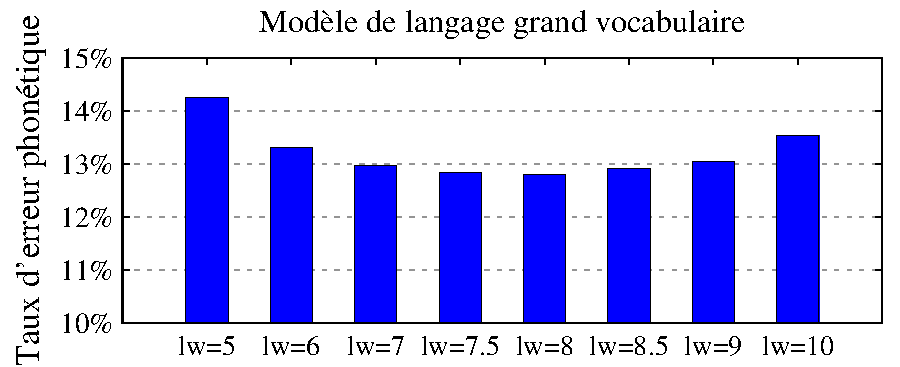
\includegraphics[scale=0.78]{images/results/results_words_lw_ESTER_v2.pdf}
\caption{Impact du poids du modèle de langage (lw) sur la performance du modèle de langage grand vocabulaire sur le corpus ESTER2}
\label{Fig:ML-W-lw-ESTER2}
\end{figure}

Le tableau \ref{Tab:W-PER} compare les performances de décodage phonétique obtenues sur les deux corpus audio ESTER2 et ETAPE, en utilisant un poids du modèle de langage égal à 8. 
Une différence de performance de 4\% (en absolu) est observée entre le contexte de parole préparée (ESTER2) et le contexte de parole spontanée (ETAPE). Il y a un manque d'adéquation entre les données textuelles utilisées pour apprendre le modèle de langage et les discours spontanés : d'un coté les modèles de langage sont appris sur des données textuelles correctes pour assurer la plus grande cohérence entre les mots reconnus par le système, et de l'autre coté une parole spontanée inclut des hésitations, répétitions, manque ou perte de cohérence.   

\begin{table}[h!]
\centering
\begin{tabular}{|r|r|r|r|r|}
\hline
\textbf{Corpus} 	&  \textbf{PER}	&  \textbf{Ins}	& \textbf{Del}	& \textbf{Sub}	\\ \hline
ESTER2			& 12,80\%	& 2,40\%	& 4,84\%	& 5,56\%	\\ \hline
ETAPE			& 16,78\%	& 2,57\%	& 7,02\%	& 7,19\%	\\ \hline
\end{tabular}
\caption{Taux d'erreur phonétique (PER) obtenus avec le modèle de langage grand vocabulaire (basé sur des mots)}
\label{Tab:W-PER}
\end{table}

Le modèle de langage grand vocabulaire est utilisé dans cette analyse comme la référence d'une performance maximale. 
Un tel modèle ne peut pas être utilisé dans un système embarqué en raison de sa taille trop importante, mais il établit la performance cible. 


%%%%%%%%%%%%%%%%%%%%%%%%%%%%%%%%%%%%%%%%%%%%%%%%
\hiddensubsection{Phonèmes}
%%%%%%%%%%%%%%%%%%%%%%%%%%%%%%%%%%%%%%%%%%%%%%%%

Un modèle de langage phonétique a été appris à partir des transcriptions phonétiques des ensembles d'apprentissage des corpus ESTER2, ETAPE et EPAC (corpus EEE). Les transcriptions phonétiques sont obtenues par alignement forcé entre les sources audio et les transcriptions manuelles correspondantes (en mots). 
L'alignement forcé sélectionne pour chaque mot la variante de prononciation qui correspond le mieux au signal (respectant ainsi la realisation par le locuteur des événements français de liaison et réduction), et identifie les segments temporels correspondant à chaque mot (et à chaque phonème) présent dans la transcription manuelle de référence.
La liste des phonèmes français est présentée dans le tableau \ref{Tab:Lex_P} en annexe.

Le modèle de langage résultant contient 40 1-grammes, 1 343 2-grammes et 29 978 3-grammes (cf. le tableau \ref{Tab:LMs_PSM} en annexe).

Les taux d'erreur phonétique obtenus avec différents poids du modèle de langage phonétique sur le corpus ESTER2 sont affichés dans la figure \ref{Fig:ML-P-lw-ESTER2}. 
La meilleure valeur pour le poids du modèle de langage est égale à 5. 

\begin{figure}[h!]
\centering
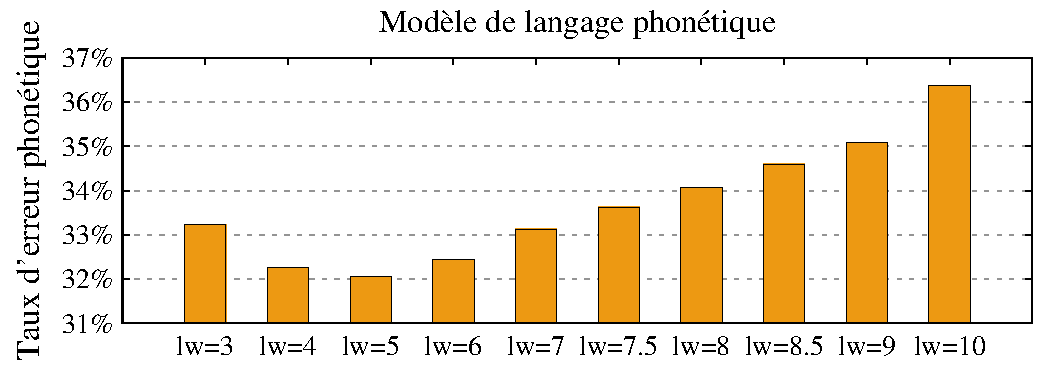
\includegraphics[scale=0.78]{images/results/results_phones_lw_ESTER_v3.pdf}
\caption{Impact du poids du modèle de langage (lw) sur la performance du modèle de langage phonétique sur le corpus ESTER2}
\label{Fig:ML-P-lw-ESTER2}
\end{figure}

Le tableau \ref{Tab:P-PER} compare les performances du décodage phonétique obtenues sur les deux corpus audio ESTER2 et ETAPE, en utilisant un poids du modèle de langage égal à 5. 
La différence de performance entre le contexte de parole préparée (ESTER2) et le contexte de parole spontanée (ETAPE) est de 1,5\%. 

\begin{table}[h!]
\centering
\begin{tabular}{|r|r|r|r|r|}
\hline
\textbf{Corpus} 	& \textbf{PER}	&  \textbf{Ins}	& \textbf{Del}	& \textbf{Sub}	\\ \hline
ESTER2			& 32,06\%	& 3,06\%	& 10,30\%	& 18,70\%	\\ \hline
ETAPE			& 33,56\%	& 2,90\%	& 12,17\%	& 18,50\%	\\ \hline
\end{tabular}
\caption{Taux d'erreur phonétique (PER) obtenus avec le modèle de langage basé sur phonèmes}
\label{Tab:P-PER}
\end{table}

L'utilisation de ce type d'unité lexicale minimise la taille du vocabulaire (moins de 40 unités phonétiques pour la langue française) et donc la taille du modèle de langage. 
Ce type de modèle pourrait être utilisé dans un système embarqué, mais malheureusement, il n'offre pas des bonnes performances.

%%%%%%%%%%%%%%%%%%%%%%%%%%%%%%%%%%%%%%%%%%%%%%%%
\hiddensubsection{Syllabes}
\label{Sec:Syllabes}
%%%%%%%%%%%%%%%%%%%%%%%%%%%%%%%%%%%%%%%%%%%%%%%%

La syllabe est une unité lexicale plus grande que le phonème, composée de phonèmes et qui modélise la manière de prononcer les mots.

Pour obtenir une liste de syllabes, des règles de syllabation ont été appliquées sur les suites de phonèmes résultant de l'alignement forcé du corpus d'apprentissage EEE, respectant ainsi les prononciations réelles (qui permettent de prendre en compte la prononciation ou non du e-muet, les liaisons et les réductions de manière réaliste). 

La syllabation employée repose sur les règles de syllabation décrites dans \cite{Bigi:2010} qui précisent qu'une syllabe contient une seule voyelle et qu'une pause désigne la frontière d'une syllabe. Les règles sont associées à différentes séquences de classes phonétiques (séquences commençant et se terminant par une voyelle) et définissent la position de la frontière entre syllabes. L'application de ces règles sur une suite de phonèmes permet d'obtenir une suite de syllabes. 

Une classe phonétique contient des sons qui partagent au moins une caractéristique phonétique. 
Généralement, les phonèmes sont répartis dans les classes suivantes~: voyelles, semi-voyelles, liquides, nasales, occlusives, affriquées et fricatives \cite{Ladefoged:1996}. 
Dans l'approche mise en œuvre, seulement 5 classes sont utilisés : voyelles (V), semi-voyelles (G), liquides (L), obstruents (O) et bruits/silences (\#). 

\begin{table}[h!]
\centering
\begin{tabular}{|c|c|c|rl|}
\hline
\textbf{Type de règle} & \specialcell{\textbf{Séquence} \\\textbf{de phonèmes}} & \specialcell{\textbf{Position} \\\textbf{de coupure}} & \multicolumn{2}{c|}{\specialcell{\textbf{Séquence} \\\textbf{de syllabes}}} \\ \hline
GENRULE 	& VV 			& 0		& V   & V		\\ \hline
GENRULE 	& VXV 			& 0 		& V   & XV		\\ \hline	
GENRULE 	& VXXV 			& 1		& VX & XV		\\ \hline
EXCRULE 	& VGGV 			& 0		& V   & GGV		\\ \hline
\end{tabular}
\caption{Quelques exemples des règles de syllabation}
\label{Tab:exRS}
\end{table}


Le tableau \ref{Tab:exRS} donne quelques exemples de règles de syllabation (plus de détails sur l'outil de syllabation sont disponibles dans l'annexe \ref{Ann:Syllabation}). %`\nameref{Sec:Ann-Syl}'). 
Dans les règles générales (GENRULE) la lettre $V$ indique un phonème appartenant à la classe phonétique de voyelles et la lettre $X$ indique un phonème appartenant à n'importe quelle autre classe. Dans les règles des exceptions (EXCRULE) la position de coupure dépend aussi de la classe phonétique des non-voyelles. 
Si une séquence de phonèmes correspond à une règle d'exception, c'est celle ci qui est appliquée et non la règle générale. 

\begin{figure}[h!]
\centering
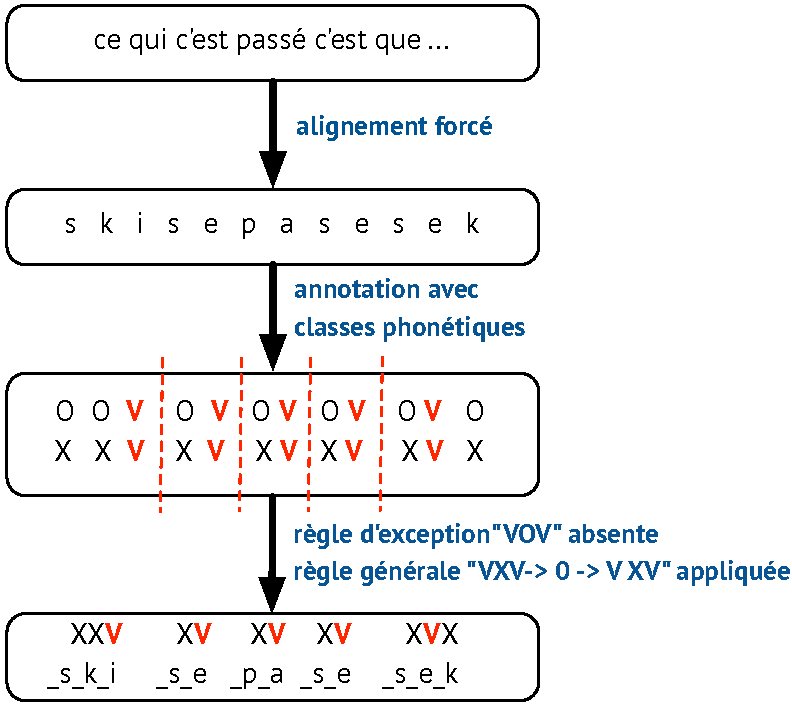
\includegraphics[scale=0.6]{images/pictures/syllabation.pdf}
\caption{Exemple de syllabation}
\label{Fig:ExSyl}
\end{figure}

Prenons l'exemple donné dans la figure \ref{Fig:ExSyl}. 
La séquence de mots ``ce qui c'est passé c'est que'' est décomposée en phonèmes par alignement forcé. 
La séquence des phonèmes correspondant à la prononciation des mots, ``\textipa{s} \textipa{k} \textipa{i} \textipa{s} \textipa{e} \textipa{p} \textipa{a} \textipa{s} \textipa{e} \textipa{s} \textipa{e} \textipa{k}'', est ensuite annotée avec ses classes phonétiques ``O O V O V O V O V O V O''. 
Pour déterminer les règles de syllabation à appliquer, les séquences qui commencent et se terminent par une voyelles sont identifiées. 
Cet exemple contient seulement des séquences de type ``V O V''. 
En l'absence d'une règle d'exception concernant une occlusion entourée par des voyelles (``V O V''), la règle générale ``VXV $\rightarrow$ 0 $\rightarrow$ V XV'' est appliquée. 
La séquence de syllabes résultante est ``\_\textipa{s}\_\textipa{k}\_\textipa{i} \ \ \ \_\textipa{s}\_\textipa{e} \ \ \ \_\textipa{p}\_\textipa{a} \ \ \ \_\textipa{s}\_\textipa{e} \ \ \ \_\textipa{s}\_\textipa{e}\_\textipa{k}''. 
La notation des syllabes repose sur des tirets bas entre les phonèmes composants; un tiret bas est aussi utilisé comme préfixe pour différencier les mots de syllabes (comme par exemple le mot `a' et la syllabe `\_\textipa{a}').  

Cette approche est facile à utiliser. Cependant, elle pose quelques problèmes. 

Un premier problème est lié aux segments de silence ou de bruit reconnus par le décodeur. 
Selon les règles de syllabation, un segment de non parole (silence ou bruit) désigne la frontière d'une syllabe. 
En conséquence, les silences/bruits divisent la séquence de phonèmes en plusieurs sous-séquences de phonèmes (entourées par des silences ou des bruits). 
Il peut arriver que le décodeur reconnaisse un petit mot entre deux silences et que la prononciation de ce petit mot corresponde à une consonne (par exemple `ce $\rightarrow$ \textipa{s}'). 
En conséquence, ce mot isolé va être considéré (à tort) comme une syllabe, alors qu'il ne contient pas de voyelle. 
Pour résoudre ce problème, les séquences sans voyelles ne sont pas incluses dans le lexique des syllabes et sont traitées comme des unités inconnues <unk> par le modèle de langage.

Un deuxième problème est lié à l'absence de voyelles. 
En regardant l'exemple précédent (figure \ref{Fig:ExSyl}) de plus près, nous pouvons remarquer que certains phonèmes manquent dans la transcription phonétique, et plus précisément, certaines voyelles (e-muets), en raison d'une vitesse d'élocution trop élevée ou d'une erreur de l'alignement forcé. 
C'est le cas du mot `ce' - qui n'est représenté que par la consonne `s', et du mot `que' - qui n'est représenté que par la consonne `k'. 
Étant donné que les règles de syllabation sont principalement basées sur la position des voyelles, et qu'il y a des voyelles manquantes dans la transcription phonétique, la séquence de syllabes résultante présente quelques ``anomalies''. La syllabe `\_\textipa{s}\_\textipa{k}\_\textipa{i}' devrait normalement être séparée en deux syllabes `\_\textipa{s}\_\textipa{@}' et `\_\textipa{k}\_\textipa{i}', et pareil pour la syllabe `\_\textipa{s}\_\textipa{e}\_\textipa{k}' - `\_\textipa{s}\_\textipa{e}' et `\_\textipa{k}\_\textipa{@}'. 
En conséquence, en appliquant les règles de syllabation, nous pouvons obtenir non seulement des syllabes, mais aussi des pseudo-syllabes, qui peuvent être définies comme des groupes de phonèmes qui ne devraient pas appartenir à une seule syllabe. 
Dans nos expériences, ces pseudo-syllabes atteignent des longueurs supérieures à 6 phonèmes. 

\begin{figure}[h!]
\centering
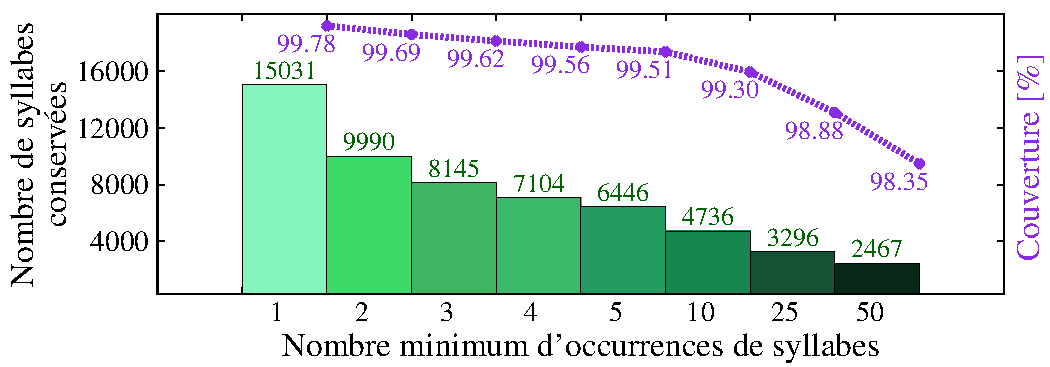
\includegraphics[scale=0.7]{images/results/couverture_syllables_minocc.pdf}
\caption{Nombre de syllabes par rapport à leur fréquence d'occurrence}
\label{Fig:s-minocc}
\end{figure}

Pour réduire le nombre de ces pseudo-syllabes, nous avons choisi de filtrer les syllabes par rapport à leur nombre d'occurrences, et de ne conserver que les plus fréquentes. Dans les expériences, les syllabes vues au moins \{1, 2, 3, 4, 5, 10, 25 ou 50\} fois dans le corpus d'apprentissage sont conservées et les autres sont ignorées. 

Le nombre de syllabes et la couverture obtenue en fonction du seuil sur le nombre minimum d'occurrences de syllabes sont affichés dans la figure \ref{Fig:s-minocc}. 
Le nombre de syllabes conservées varie entre 15 000 et 2 000 syllabes, avec une couverture de 99,78\% à 98,35\% des occurrences. 
Les syllabes qui ont été vues moins de 3 fois dans le corpus d'apprentissage représentent presque la moitié du nombre total de syllabes  différentes (46\%), mais elles ont un faible impact sur la couverture de syllabes (0,16\%). 
En les ignorant, nous pouvons conserver un nombre restreint de syllabes (8 100 syllabes) tout en assurant une bonne couverture (99,62\% des occurrences).

\begin{figure}[h!]
\centering
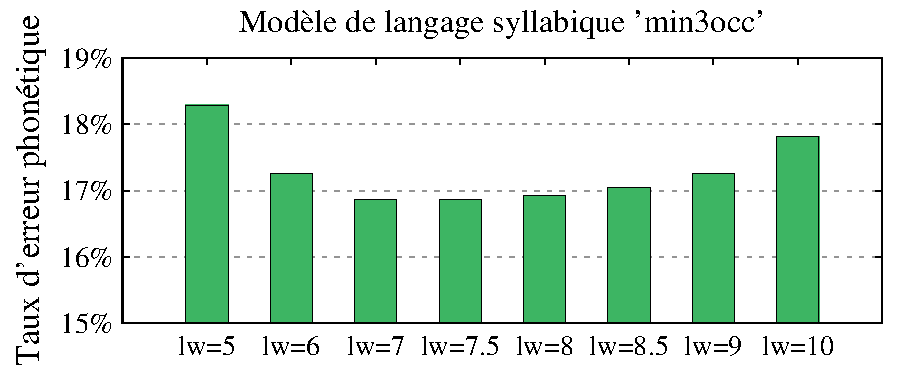
\includegraphics[scale=0.72]{images/results/results_syllables_lw_ESTER_v2.pdf}
\caption{Impact du poids du modèle de langage (lw) sur la performance du modèle de langage syllabique `min3occ' sur le corpus ESTER2}
\label{Fig:PER-s-lw}
\end{figure}

Les taux d'erreur phonétique obtenus avec différents poids du modèle de langage syllabique basé sur les syllabes qui ont une fréquence d'au moins 3 occurrences (`min3occ') sur le corpus ESTER2 sont affichés dans la figure \ref{Fig:PER-s-lw}. La meilleure valeur pour le poids du modèle de langage est égale à 7.

\begin{figure}[h!]
\centering
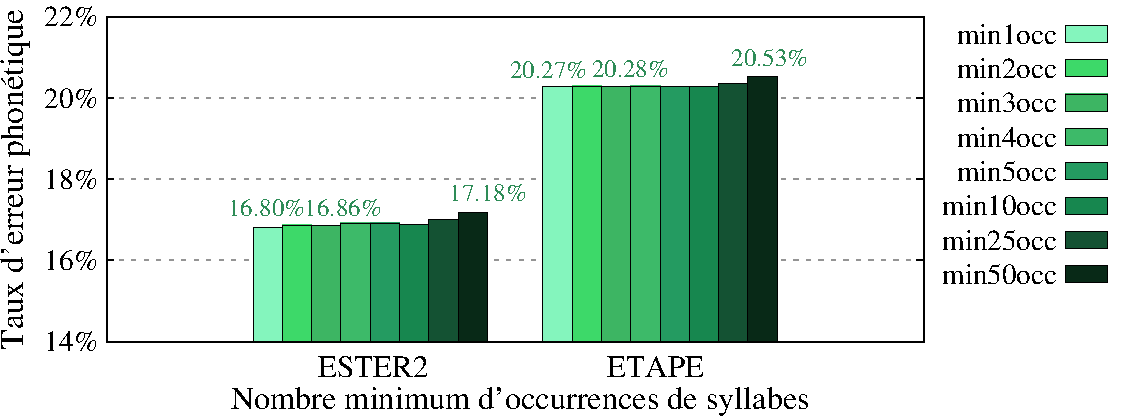
\includegraphics[scale=0.72]{images/results/results_minocc.pdf}
\caption{Taux d'erreur phonétique obtenus avec les modèles de langage syllabiques sur les corpus ESTER2 et ETAPE}
\label{Fig:PER-s}
\end{figure}

Nous avons ensuite analysé les taux d'erreur phonétique obtenus avec les différents modèles de langage syllabiques sur les corpus ESTER2 et ETAPE, en utilisant un poids du modèle de langage égal à 7 (cf. Fig. \ref{Fig:PER-s}). La performance du modèle de langage syllabique semble peu sensible au nombre de syllabes dans le lexique : il y a une différence de performance de seulement 0,33\% entre le modèle de langage comprenant toutes les syllabes (`min1occ') et le modèle de langage comprenant les syllabes ayant une fréquence de minimum 50 occurrences (`min50occ').  La différence de performance entre le contexte de parole préparée (ESTER2) et le contexte de parole spontanée (ETAPE) est de 3,5\%.  

L'utilisation de ce type d'unité lexicale conduit à une taille raisonnable pour le lexique (8 100 syllabes vues au moins 3 fois) et pour le modèle de langage. 
Ce type de modèle peut être utilisé dans un système embarqué, tout en offrant de bonnes performances de décodage phonétique ($\sim$17\% PER).


%%%%%%%%%%%%%%%%%%%%%%%%%%%%%%%%%%%%%%%%%%%%%%%%%%%%%%%%%%
\hiddensubsection{Comparaison des 3 unités lexicales}
%%%%%%%%%%%%%%%%%%%%%%%%%%%%%%%%%%%%%%%%%%%%%%%%%%%%%%%%%%

L'impact des modèles de langage et des choix de lexique a été étudié en vue d'établir le meilleur compromis pour une solution embarquée. 

\begin{table}[h!]
\centering
\begin{tabular}{|l|r|}
\hline
Modèle de langage	& meilleur poids \\ \hline
ML=phonèmes		&	lw=5	\\ \hline
ML=syllabes		&	lw=7	\\ \hline
ML=mots			&	lw=8	\\ \hline
\end{tabular}
\caption{Valeur optimale du poids de modèle de langage pour les 3 unités lexicales sur le corpus ESTER2}
\label{Tab:choixLW}
\end{table}

Le poids de modèle de langage qui minimise le taux d'erreur phonétique pour chaque type d'unité lexicale est rappelé dans le tableau \ref{Tab:choixLW}. 
La valeur optimale du poids du modèle augmente avec la taille des unités lexicales : $lw=5$ pour le modèle phonétique, $lw=7$ pour le modèle syllabique `min3occ' et $lw=8$ pour le modèle grand vocabulaire. Ces valeurs indiquent l'importance du modèle de langage par rapport au modèle acoustique : le système privilégie les modèles de langage seulement quand ils sont détaillés.

\begin{figure}[h!]
\centering
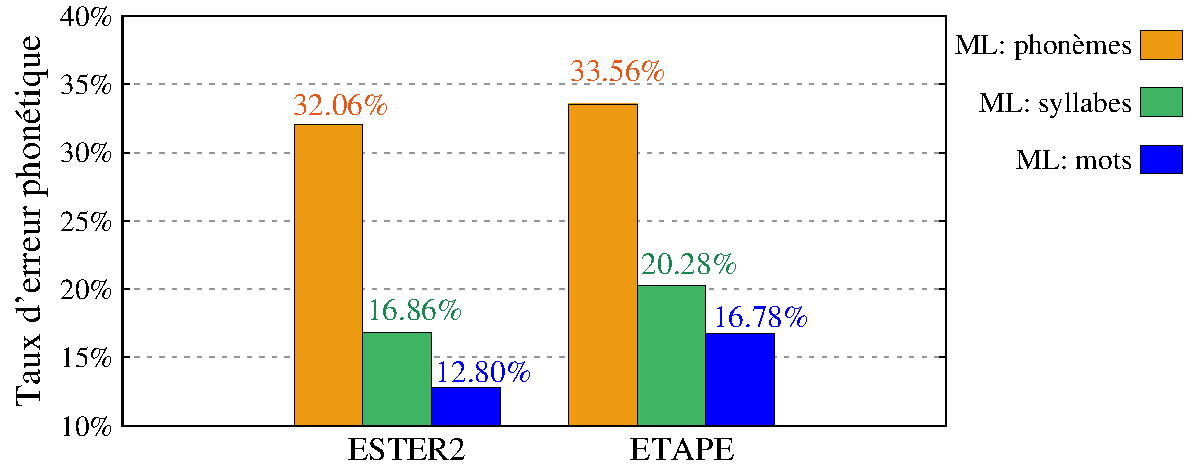
\includegraphics[scale=0.69]{images/results/overallResults_3LM.pdf}
\caption{Comparaison des taux d'erreur phonétique obtenus avec les 3 unités lexicales}
\label{Fig:overall-3LM}
\end{figure}

Les taux d'erreur de reconnaissance (mesurés sur les phonèmes) obtenus sur les données de développement des corpus ESTER2 et ETAPE sont présentés dans la figure \ref{Fig:overall-3LM}. 
Le taux d'erreur phonétique obtenu avec le modèle de langage syllabique (qui utilise les syllabes vues au moins trois fois dans le corpus d'apprentissage) n'est que de 4\% plus mauvais (en valeur absolue) que le taux d'erreur obtenu avec le système de reconnaissance grand vocabulaire, et bien meilleur que le taux d'erreur obtenu avec le modèle de langage phonétique.

Une analyse détaillée des performances de reconnaissance en fonction du rapport signal-à-bruit et de la vitesse d'élocution a également été effectuée. 
Les valeurs de rapport signal-à-bruit ont été obtenues à partir des valeurs moyennes des coefficients MFCC C0 calculés (par l'outil \textit{sphinx\_fe}) sur les voyelles et sur les zones de non-parole (silence ou bruit), converties ensuite en dB (cf. eq. \ref{Eq:SnR-dB}). 
La vitesse d'élocution est définie par le nombre de voyelles par seconde (ce qui correspond aussi au nombre de syllabes par seconde).
Les intervalles de rapport signal-à-bruit et les intervalles de vitesse d'élocution ont été découpés de manière arbitraire afin d'obtenir des sous-ensembles de données des tailles équivalentes.

\begin{equation}
SNR_{dB}=10\ log_{10}\frac{P_{signal}}{P_{bruit}} \cong 10 \left ( \frac{ln(\bar{C_0}_{voyelle})}{ln(10)} - \frac{ln(\bar{C_0}_{bruit})}{ln(10)} \right )
\label{Eq:SnR-dB}
\end{equation}


Les différentes unités lexicales ont des comportement similaires : la performance de reconnaissance s'améliore (le taux d'erreur baisse) avec l'augmentation du rapport signal-à-bruit et avec la diminution de la vitesse d'élocution (cf. Fig. \ref{Fig:SNR-SR}). 

\begin{figure}[h!]
\begin{subfigure}{\textwidth}
\centering
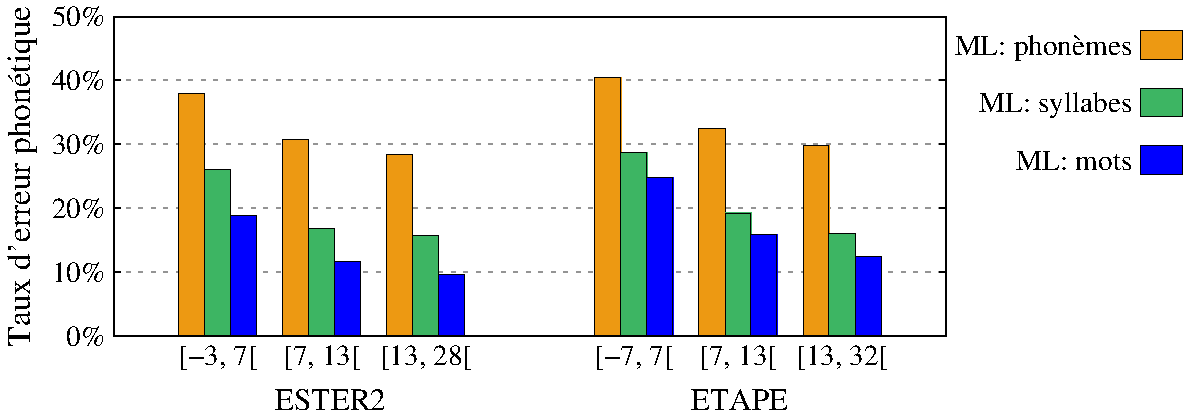
\includegraphics[scale=0.69]{images/results/wPER-SnR-3LM.pdf}
\caption{Rapport signal-à-bruit {[}dB{]}}
\end{subfigure}
\begin{subfigure}{\textwidth}
\centering
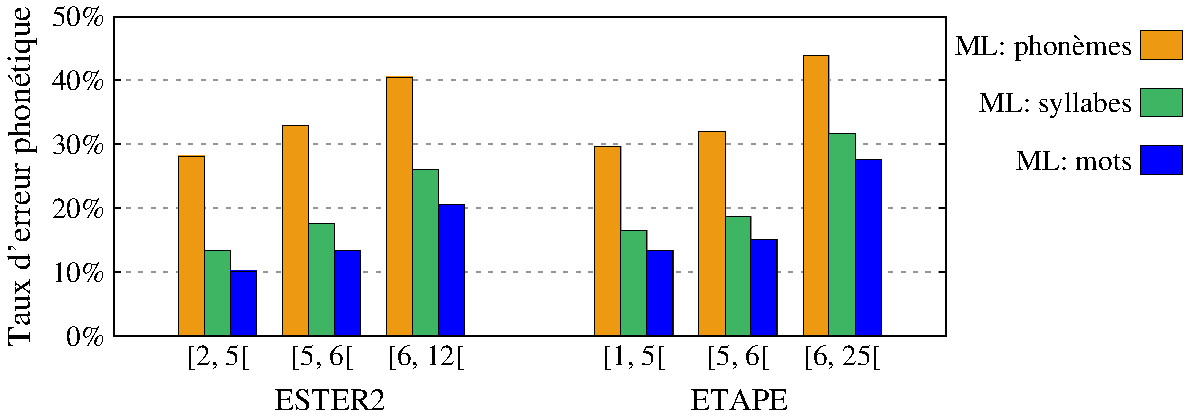
\includegraphics[scale=0.69]{images/results/wPER-SR-3LM.pdf} 
\caption{Vitesse d'élocution {[}\#syllabes/seconde{]}}
\end{subfigure}
\caption{Taux d'erreur phonétique obtenus sur les corpus ESTER2 et ETAPE, en fonction du rapport signal-à-bruit (a) et de la vitesse d'élocution (b)}
\label{Fig:SNR-SR}
\end{figure}

Les performances obtenues sur le corpus ETAPE avec le modèle de langage grand vocabulaire par rapport au différents intervalles de rapports signal-à-bruit et de vitesse d'élocution sont présentées dans le tableau \ref{Tab:comb-SnR-SR}. 
Des écarts importants de performance sont observés entre les conditions les plus favorables (signal peu bruité, i.e. rapport signal-à-bruit élevé, et vitesse d'élocution basse) et les conditions les moins favorables (signal bruité, et vitesse d'élocution élevée). 

\begin{table}[h!]
\centering
\begin{tabular}{r|r|r|r|r|}
\multicolumn{1}{c}{} & \multicolumn{1}{c}{}		& \multicolumn{3}{c}{Vitesse d'élocution} 	\\ \cline{3-5}
\multicolumn{1}{c}{} & \multicolumn{1}{c|}{}		& [2, 5[ 	& [5, 6[	& [6, 25[	\\ \cline{2-5}
\multirow{3}{*}{Rapport signal-à-bruit}	& [-3, 7[	& 14,49		& 17,89		& 25,97		\\ \cline{2-5}
					& [7, 13[	& 12,76		& 13,05		& 17,39		\\ \cline{2-5}
					& [13, 28[	&  8,89		& 10,23		& 15,37		\\ \cline{2-5}
\end{tabular}
\caption{Taux d'erreur phonétique obtenus avec les modèles de langage grand vocabulaire sur les corpus ETAPE en fonction du rapport signal-à-bruit et de la vitesse d'élocution}
\label{Tab:comb-SnR-SR}
\end{table}


%=====================================================================================
\section{Heuristiques de décodage}
\label{Sec:HD}
\renewcommand{\rightmark}{Heuristiques de décodage}
%===================================================================================

Une analyse complémentaire a été menée pour évaluer l'impact de la taille des modèles acoustiques sur les performances de reconnaissance. 

Comme indiqué précédemment (section \ref{Sec:HMM}), les deux principaux paramètres qui influent sur la taille globale du modèle acoustique sont le nombre total de sénones (le nombre de densités de probabilité partagées entre les modèles contextuels des sons), et le nombre de gaussiennes par densité.

Les modèles obtenus en modifiant ces paramètres sont plus ou moins détaillés. 
Un modèle peu détaillé (peu de sénones, peu de gaussiennes par densité) occupera moins de place en mémoire, mais sera peu performant. 
L'augmentation du nombre de gaussiennes par densité, et du nombre de sénones permet d'améliorer la qualité de la modélisation, et donc les performances de reconnaissance, mais le modèle prendra plus de place en mémoire, et coutera aussi plus cher en CPU pour le décodage.

\begin{table}[h!]
\centering
\begin{tabular}{r|rl|rr|rr|rr|}
\multicolumn{3}{c}{}  	& \multicolumn{6}{c}{\textbf{\#sénones}} \\ \cline{4-9}	
\multicolumn{3}{c|}{}  	& \multicolumn{2}{c|}{2 500 sen} & \multicolumn{2}{c|}{5 000 sen} & \multicolumn{2}{c|}{7 500 sen}	 	  \\ \cline{2-9}
\parbox[t]{2mm}{\multirow{5}{*}{\rotatebox[origin=c]{90}{\textbf{\#gaussiennes}}}} 	& 8 g   &	& 20 000  & [6 Mo]	& 40 000  & [13 Mo]	& 60 000  & [19 Mo]  \\ \cline{2-9}
											& 16 g  &	& 40 000  & [13 Mo]	& 80 000  & [25 Mo]	& 120 000 & [37 Mo]  \\ \cline{2-9}
											& 32 g  &	& 80 000  & [26 Mo]	& 160 000 & [50 Mo]	& 240 000 & [74 Mo]  \\ \cline{2-9}
											& 64 g  &	& 160 000 & [51 Mo] 	& 320 000 & [100 Mo]	& 480 000 & [148 Mo] \\ \cline{2-9}
											& 64 g  & (H/F)	& 320 000 & [102 Mo]  	& 640 000 & [200 Mo]	& 960 000 & [296 Mo] \\ \cline{2-9}
\end{tabular}
\caption{Taille des modèles acoustique}
\label{Tab:tailleAMs}
\end{table}


Plusieurs modèles acoustiques ont été évalués, en considérant différents nombres de sénones (2500, 5000 ou 7500) et différents nombres de gaussiennes par densité (8, 16, 32 ou 64). 
Leur nombre total de paramètres et leur taille sont indiqués  dans le tableau \ref{Tab:tailleAMs}. Le modèle `64g(H/F)' représente le modèle acoustique avec 64 gaussiennes adaptées à la parole des hommes (H) et autant à la parole des femmes (F).


\begin{figure}[h!]
\centering
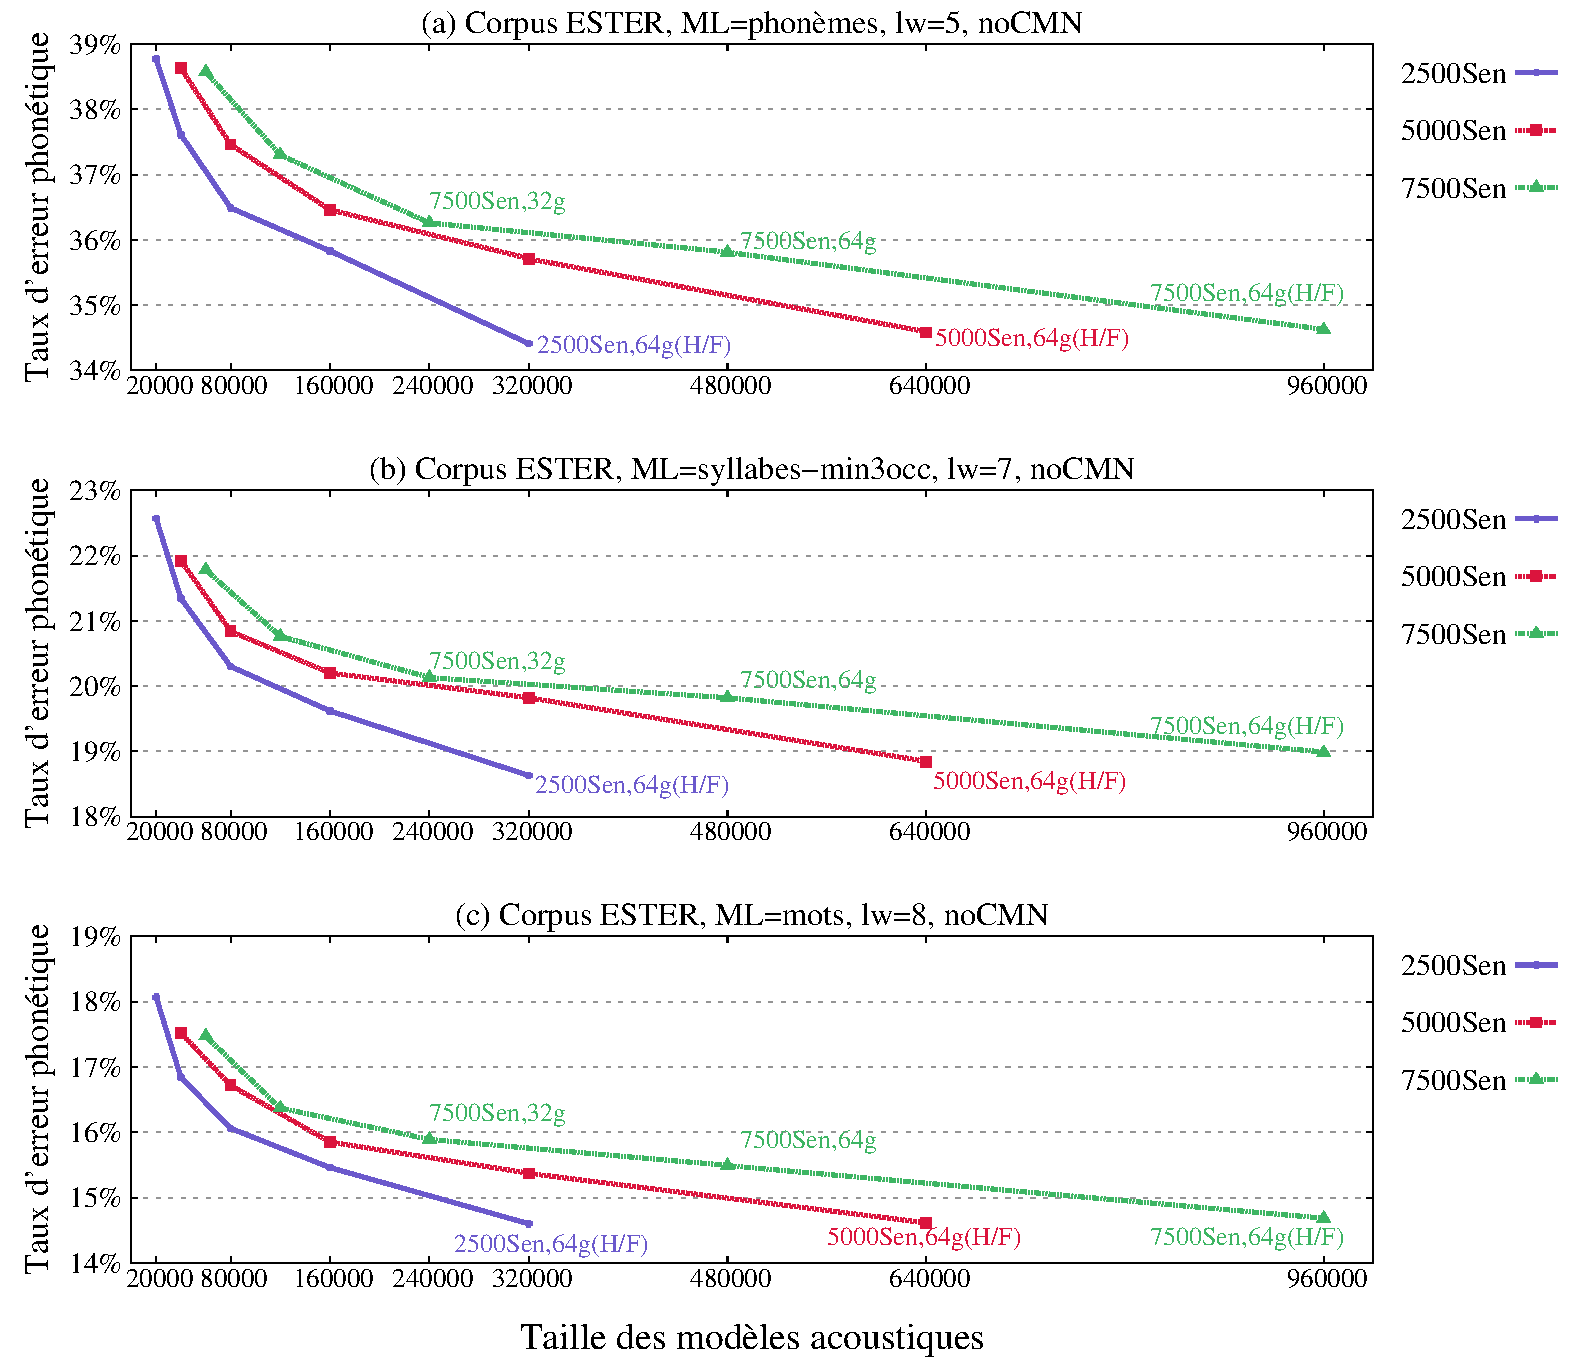
\includegraphics[scale=0.54]{images/results/results_AM_ESTER.pdf}
\caption{Taux d'erreur phonétique sur le corpus ESTER2 obtenus avec différentes tailles de modèles acoustiques (tailles exprimées en nombre total de gaussiennes), en utilisant un modèle de langage phonétique (a), syllabique (b) ou grand vocabulaire (c)}
\label{Fig:tailleAM-PER}
\end{figure}


La figure \ref{Fig:tailleAM-PER} montre les résultats obtenus en décodage phonétique sur le corpus ESTER2 en considérant les modèles de langage phonétique, syllabique et grand vocabulaire. 
L'axe horizontale indique le nombre total des paramètres des différentes modèles acoustiques ayant entre 20K gaussiennes (8 gaussiennes par densité, 2500 états partagés) et 960K gaussiennes (64 gaussiennes par densité, 7500 états partagés, adaptation homme/femme). 
Les résultats montrent qu'un nombre important des gaussiennes par densité est plus important qu'un nombre élevé de sénones. 
Les résultats sont similaires pour tous les 3 unités lexicales. 

De nombreux critères viennent aussi impacter les performances de reconnaissance et le temps CPU nécessaire pour le décodage. Ils sont liés aux heuristiques de l'algorithme de décodage. Plus les heuristiques sont restreintes, moins le décodeur explore de solutions possibles; en conséquence cela coûte moins cher en calcul, mais c'est au détriment du taux d'erreur. 
Il est aussi important de souligner que le temps de calcul fluctue d'un énoncé à un autre. Le temps de réponse à tendance à être plus important lorsque l'on traite un signal de mauvaise qualité.



%%%%%%%%%%%%%%%%%%%%%%%%%%%%%%%%%%%%%%%%%%%%%%%%%%%%%%%%%%%%%%%%%%%%%%%%%%%%
\chapter{Modèles hybrides}
\renewcommand{\leftmark}{Modèles hybrides}
\renewcommand{\rightmark}{}
%%%%%%%%%%%%%%%%%%%%%%%%%%%%%%%%%%%%%%%%%%%%%%%%%%%%%%%%%%%%%%%%%%%%%%%%%%%%

Dans le projet, des entretiens effectués avec des personnes sourdes ont révélé l'intérêt d'une reconnaissance en mots \cite{Piquard:2015}. 
En effet, cette solution est la plus simple à appréhender et, contrairement à la reconnaissance en syllabes, elle ne nécessite pas d'effort supplémentaire de la part du lecteur pour regrouper les différentes syllabes en mots porteurs de sens. 
Cependant, le choix d'un modèle de langage à base des mots ne résout pas tous les problèmes. 
L'incapacité de concevoir un système qui couvre tous les mots (taille fini du lexique) et qui ne soit pas contraint par les ressources disponibles, nous a amené à proposer et développer une approche combinant des mots et des syllabes dans un seul modèle de langage, dit hybride. 
Le choix des syllabes résulte de leurs bonnes performances en décodage phonétique (cf. chapitre précédent) pour une taille limitée des modèles associés. 
Le nombre de mots peut-être ajusté en fonction des ressources disponibles.

L'utilisation d'un tel modèle de langage hybride vise à assurer une reconnaissance correcte des mots les plus fréquents et à proposer des suites de syllabes pour les segments de parole correspondant à des mots hors vocabulaire. Les syllabes devraient faciliter la compréhension des segments de parole hors vocabulaire, du moins plus facilement que de devoir interpréter une suite de petits mots dont l'une des variantes de prononciation correspond au segment de parole hors vocabulaire (ce qui est le cas le plus fréquent lorsque le lexique et le modèle de langage n'utilisent pas d'unités sous-lexicales).

En conséquence, ce chapitre analyse l'intérêt des modèles de langage hybrides pour transcrire de la parole. 

Cette partie du travail est publiée dans deux articles de conférence \cite{Orosanu2014_1, Orosanu2014_2}.

\minitoc


%===================================================================================
\section{Fabrication des modèles hybrides}
\renewcommand{\rightmark}{Fabrication des modèles hybrides}
%===================================================================================

La fabrication d'un modèle de langage hybride, combinant mots et syllabes, implique de constituer un corpus d'apprentissage qui repose sur ces deux unités lexicales. 
Pour ce faire, le vocabulaire est défini en sélectionnant les mots les plus fréquents, i.e. les mots qui apparaissent au moins $\theta$ fois dans le corpus d'apprentissage; puis les mots hors vocabulaire sont décomposés en syllabes; et les syllabes correspondantes sont alors ajoutées au lexique.

Un alignement forcé est appliqué sur les données d'apprentissage EEE, afin de déterminer quelle variante de prononciation a été effectivement utilisée pour chaque mot prononcé (fréquent ou pas). Ensuite, les mots peu fréquents (non sélectionnés par rapport au seuil choisi) sont remplacés par leur variante de prononciation résultant de l'alignement forcé. Enfin, les séquences de phonèmes ainsi obtenues, correspondant aux segments de parole entre les mots sélectionnés, sont traitées par l'outil de syllabation décrit dans le chapitre précédent.

Prenons l'exemple donnée dans la figure \ref{Fig:ExWS}. La phrase ``une femme a été blessée'' contient 4 mots fréquents \{une, femme, a, été\} et un seul mot non-fréquent \{blessée\}. Le mot ``blessée'' est remplacé par sa prononciation ``\textipa{b} \textipa{l} \textipa{e} \textipa{s} \textipa{e}" (variante résultante de l'alignement forcé), qui est ensuite découpée en deux syllabes ``\_\textipa{b}\_\textipa{l}\_\textipa{e}'' et \linebreak ``\_\textipa{s}\_ \textipa{e}". La séquence finale de mots et syllabes est alors ``une femme a été \_\textipa{b}\_\textipa{l}\_\textipa{e} \ \_\textipa{s}\_ \textipa{e}".

\begin{figure}[h!]
\centering
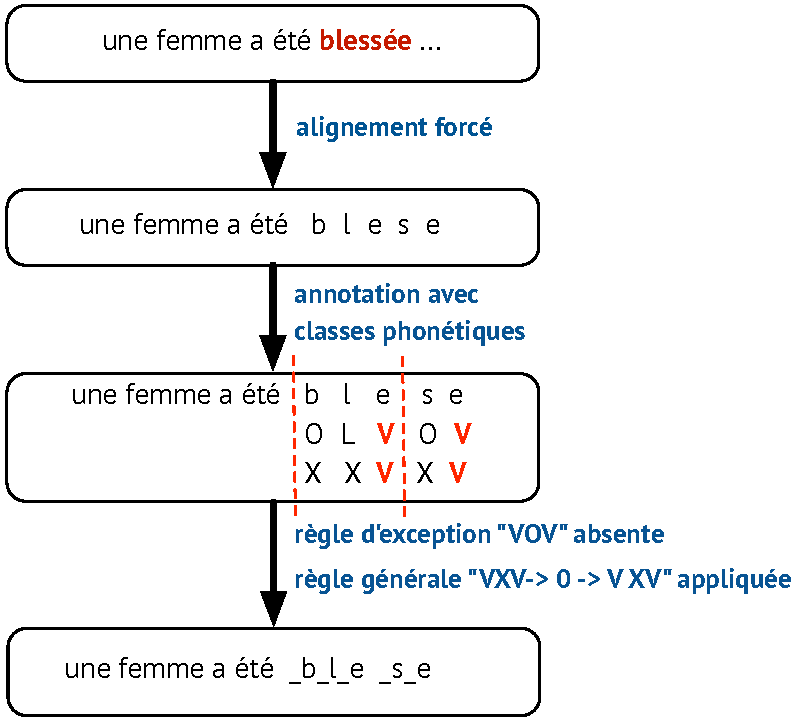
\includegraphics[scale=0.65]{images/pictures/syllabation-WS.pdf}
\caption{Préparation des données pour la fabrication des modèles de langage hybrides}
\label{Fig:ExWS}
\end{figure}

Différents seuils minimaux sur la fréquence d'occurrence des mots ont été considérés~: $\theta \in \{3, 5, 10, 25, 50, 100, 300\}$. Chaque choix de seuil entraîne la création d'une transcription différente du corpus d'apprentissage (avec un nombre différent de mots et de syllabes), et conduit à un lexique et un modèle de langage correspondant. 
Pour limiter la taille des modèles et éviter de conserver trop de pseudo-syllabes non pertinentes (cf. Sec. \ref{Sec:Syllabes}.3), seules les syllabes observées au moins trois fois dans le corpus d'apprentissage sont conservées dans les lexiques et dans les modèles de langage.

\begin{figure}[h!]
\centering
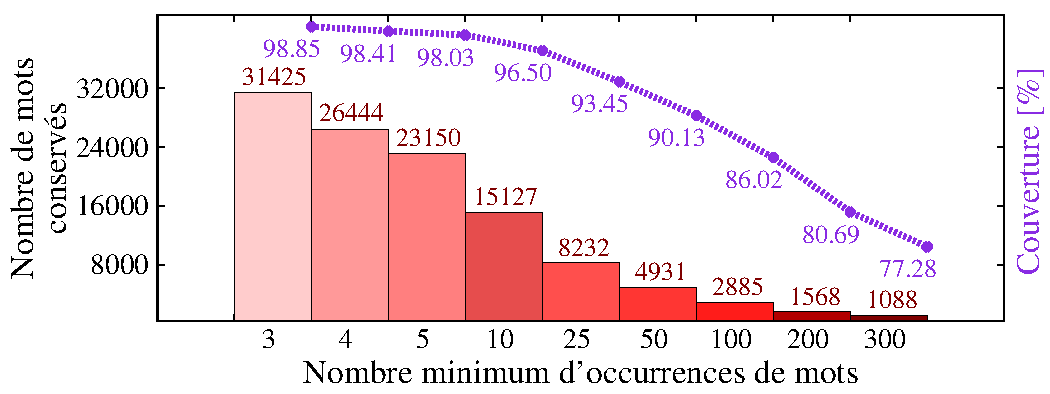
\includegraphics[scale=0.64]{images/results/couverture_ws_minocc.pdf}
\caption{Nombre et couverture des mots dans les modèles de langage hybrides}
\label{Fig:ML-WS1}
\end{figure}

Le nombre de mots et la couverture, résultant de l'application de différents seuils sur le nombre minimum d'occurrences de mots, sont présentés dans la figure \ref{Fig:ML-WS1}.
En sélectionnant les 31 000 mots les plus fréquents du corpus d'apprentissage, près de 99\% des occurrences de mots du corpus sont couvertes. 
En ne sélectionnant que les 5 000 mots les plus fréquents, le taux de couverture est encore supérieur à 90\%.

\begin{figure}[h!]
\centering
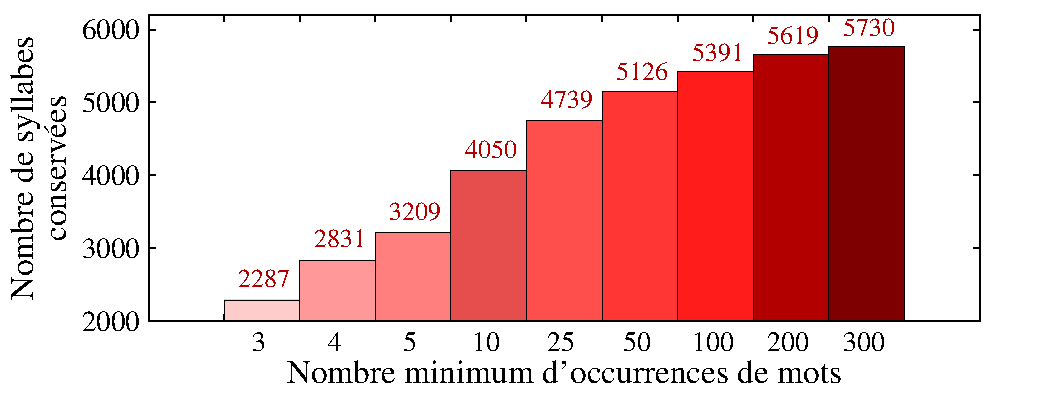
\includegraphics[scale=0.64]{images/results/couverture_ws_s_minocc.pdf}
\caption{Nombre de syllabes utilisées dans les modèles de langage hybrides}
\label{Fig:ML-WS2}
\end{figure}

La figure \ref{Fig:ML-WS2} affiche le nombre de syllabes nécessaires pour représenter les prononciations des mots non sélectionnés dans le lexique en fonction du seuil sur le  nombre minimum d'occurrences de mots. En fonction de la liste des mots sélectionnés, 2 à 6 000 syllabes sont nécessaires.  

Ces différentes sélections conduisent à des lexiques hybrides de 33 000 à 7 000 entrées (mots plus syllabes). Les modèles de langage associés comportent environ 1,8 millions de 3-grammes, pour une taille totale de 11 à 14 Mo (cf. le tableau \ref{Tab:LMs_H} en annexe).


%===================================================================================
\section{Évaluation des modèles hybrides}
\renewcommand{\rightmark}{Évaluation des modèles hybrides}
%===================================================================================

L'évaluation des modèles hybrides a comme objectif de déterminer si la combinaison de mots et de syllabes conduit néanmoins à un bon taux de reconnaissance des mots (ce qui est important pour les personnes sourdes).
Nous nous intéressons également aux taux de mots correctement reconnus (par rapport à la transcription de référence), aux taux de syllabes correctement reconnus (par rapport à l'alignement forcé de la transcription de référence) et aux taux de mots hors-vocabulaire reconnus par des syllabes. 
Nous étudions la pertinence des mesures de confiance pour identifier les mots correctement reconnus. 

%%%%%%%%%%%%%%%%%%%%%%%%%%%%%%%%%%%%%%%%%%%%%%%%
\hiddensubsection{Taux d'erreur phonétique}

La première évaluation porte sur les taux d'erreur phonétique obtenus avec les différents modèles de langage hybrides; ces taux sont affichés dans la figure \ref{Fig:ML-WS3}.
La performance du modèle de langage hybride dépend du nombre de mots conservés dans le lexique : il y a une différence de performance d'environ 1,5\% entre le modèle de langage comprenant les mots vus au moins 3 fois (`min3occ') et le modèle de langage comprenant les mots ayant au moins 300 occurrences (`min300occ').  La différence de performance entre le contexte de parole préparée (ESTER2) et le contexte de parole spontanée (ETAPE) est de 3,7\%.  

\begin{figure}[h!]
\centering
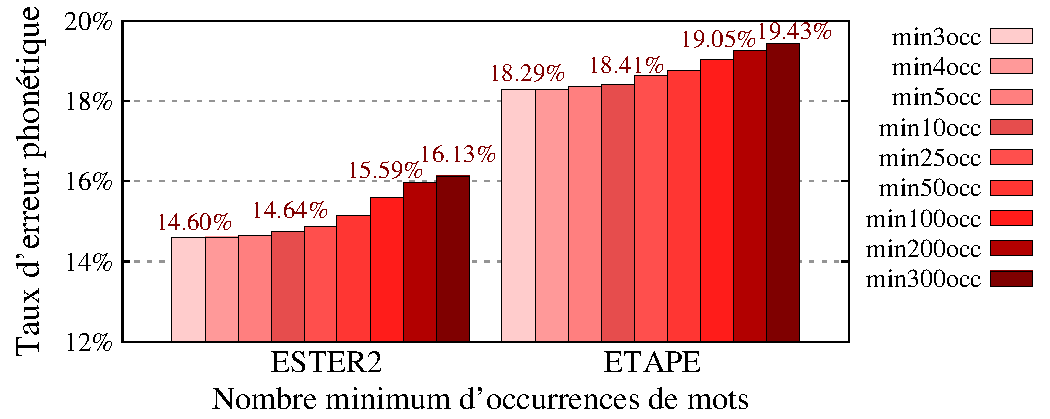
\includegraphics[scale=0.72]{images/results/results_ws_minocc.pdf}
\caption{Taux d'erreur phonétique obtenus avec les modèles de langage hybrides}
\label{Fig:ML-WS3}
\end{figure}

Comparé aux autre modèles de langage classiques (mots, phonèmes, syllabes), le modèle de langage hybride `min3occ' a une performance supérieure à celle du modèle syllabique ($\sim$2\%), mais toujours inférieure à celle du modèle grand vocabulaire ($\sim$2\%). 
Pour rappel, le modèle de langage grand vocabulaire a été appris sur une base de données contenant environ 1,7Md de mots, avec un lexique de 97K mots; alors que le modèle de langage hybride (31 000 mots et 2 000 syllabes) est appris à partir des transcriptions de données de parole correspondant à 3,4M mots plus 110K syllabes. 

\begin{figure}[h!]
\centering
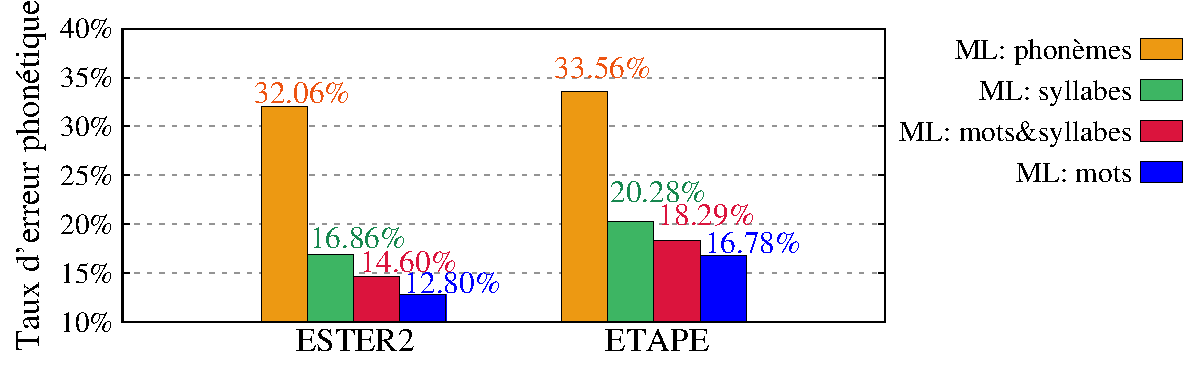
\includegraphics[scale=0.72]{images/results/overallResults_4LM.pdf}
\caption{Comparaison des taux d'erreur phonétique obtenus avec les 4 modèles de langage}
\label{Fig:overall-4LM}
\end{figure}


%%%%%%%%%%%%%%%%%%%%%%%%%%%%%%%%%%%%%%%%%%%%%%%%
\hiddensubsection{Mots et syllabes}

Étant donné que les modèles de langage hybrides mélangent des mots et des syllabes, et que nous sommes intéressés à récupérer le message porté par la parole, nous avons particulièrement analysé combien de mots sont produits par le décodeur (dans la séquence de mots et de syllabes), et parmi ces mots, combien d'entre eux sont effectivement bien reconnus.

\begin{figure}[h!]
\centering
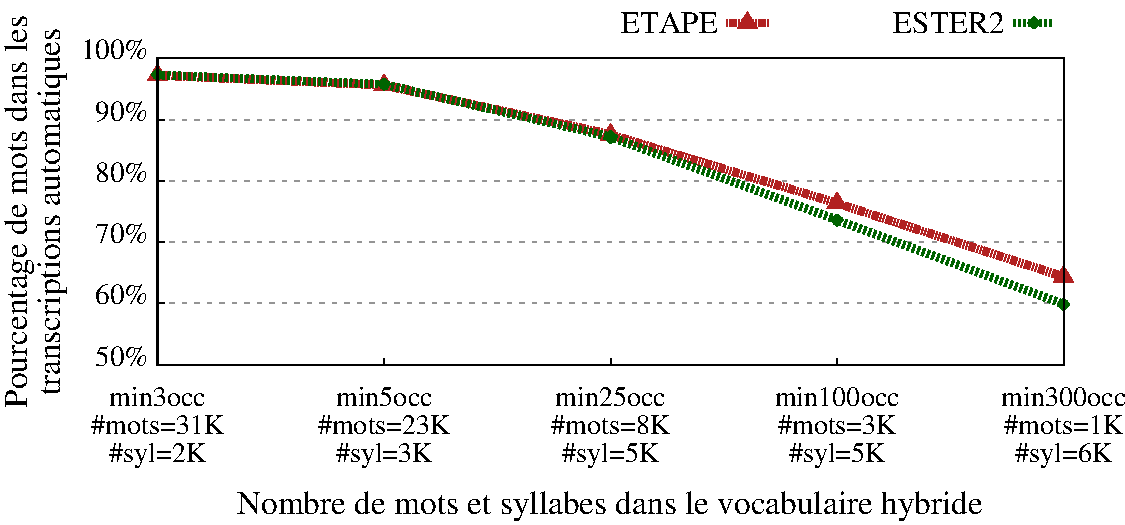
\includegraphics[scale=0.64]{images/results/wordsInWS_sv.pdf}
\caption{Taux de mots dans la séquence de mots et syllabes reconnus par les modèles hybrides}
\label{Fig:pWordsInWS}
\end{figure}

La figure \ref{Fig:pWordsInWS} affiche le pourcentage de mots produits par le décodeur en fonction des différents vocabulaires hybrides : les sorties de reconnaissance contiennent essentiellement des mots. 
Les transcriptions automatiques obtenues sur le corpus ESTER2 présentent 97\% de mots pour le plus gros modèle (`min3occ', qui a donné 40K mots et 1K syllabes) et $\sim$60\% pour le plus petit modèle (`min300occ', qui a donné 31K mots et 21K syllabes). 
Les transcriptions automatiques obtenues sur le corpus ETAPE présentent 97\% de mots pour le plus gros modèle (`min3occ', qui a donné 72K mots et 2K syllabes) et $\sim$63\% pour le plus petit modèle (`min300occ', qui a donné 59K mots et 33K syllabes).

\begin{figure}[h!]
\centering
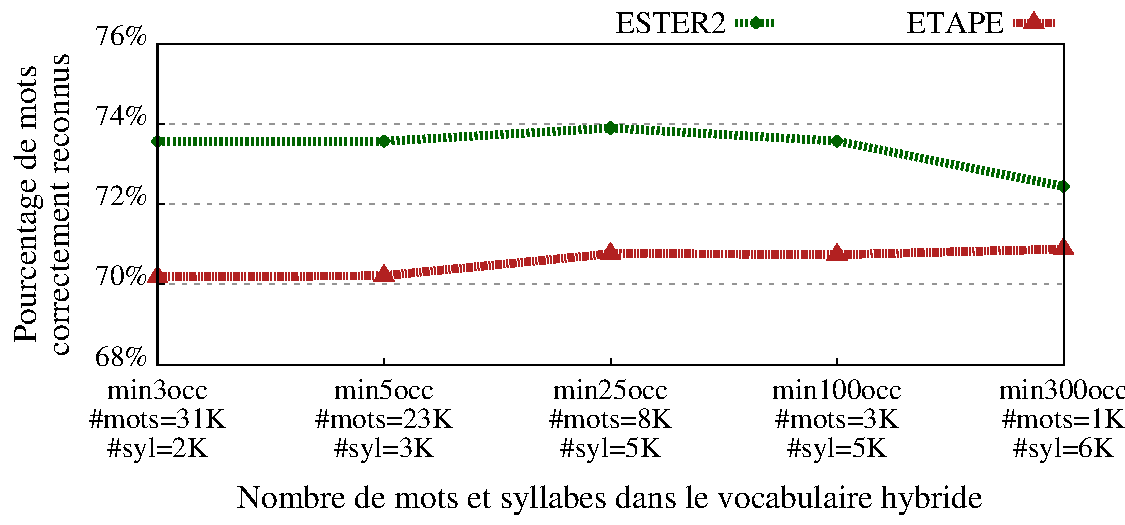
\includegraphics[scale=0.64]{images/results/correctWordsInWS_sv.pdf}
\caption{Taux de mots correctement reconnus par les modèles hybrides}
\label{Fig:cWordsInWS}
\end{figure}

Les pourcentages de mots correctement reconnus parmi les mots produits par le décodeur, en fonction des différents vocabulaires hybrides, sont présentés dans la figure \ref{Fig:cWordsInWS}. 
Ce pourcentage est obtenu en comparant les transcriptions automatiques en mots et syllabes avec l'alignement forcé (en mots) des références (\acrshort{STM}) du corpus de parole~: pour qu'un mot soit considéré comme étant bien reconnu il doit être présent dans les deux transcriptions, automatique et référence, dans le même intervalle temporel ($\pm$40ms pour tolérer les petites erreurs de segmentation ou d'alignement). Il y a en moyenne 73\% de mots bien reconnus sur le corpus ESTER2, versus 71\% sur le corpus ETAPE.

\begin{figure}[h!]
\centering
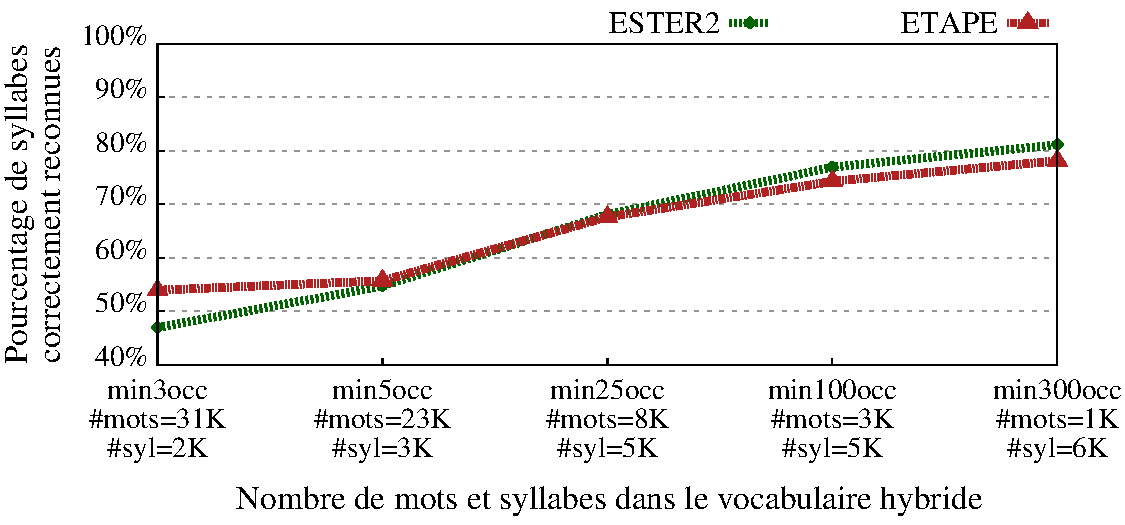
\includegraphics[scale=0.64]{images/results/correctSyllablesInWS_sv.pdf}
\caption{Taux de syllabes correctement reconnues par les modèles hybrides}
\label{Fig:cSylInWS}
\end{figure}

Le pourcentage de syllabes correctement reconnues parmi les syllabes produites par le décodeur, en fonction des différents vocabulaires hybrides, est également étudié. 
Ce pourcentage est obtenu en comparant les transcriptions automatiques en mots et syllabes avec l'alignement forcé (en phonèmes) des références (\acrshort{STM}) du corpus de parole : pour qu'une syllabe soit considérée comme étant bien reconnue, la totalité des phonèmes la composant doit être présente dans les deux transcriptions, automatique et référence, dans le même intervalle temporel ($\pm$40ms pour tolérer les petites erreurs de segmentation ou d'alignement). 
Les taux de syllabes bien reconnues varient entre 46\% et 81\% pour le corpus ESTER2 et entre 54\% et 78\% pour le corpus ETAPE  (cf. Fig. \ref{Fig:cSylInWS}).



%%%%%%%%%%%%%%%%%%%%%%%%%%%%%%%%%%%%%%%%%%%%%%%%
\hiddensubsection{Mots hors-vocabulaire}

Une des raisons de l'implémentation d'un modèle hybride est liée à son pouvoir de transcrire les mots hors-vocabulaire par des syllabes. 

\begin{figure}[h!]
\centering
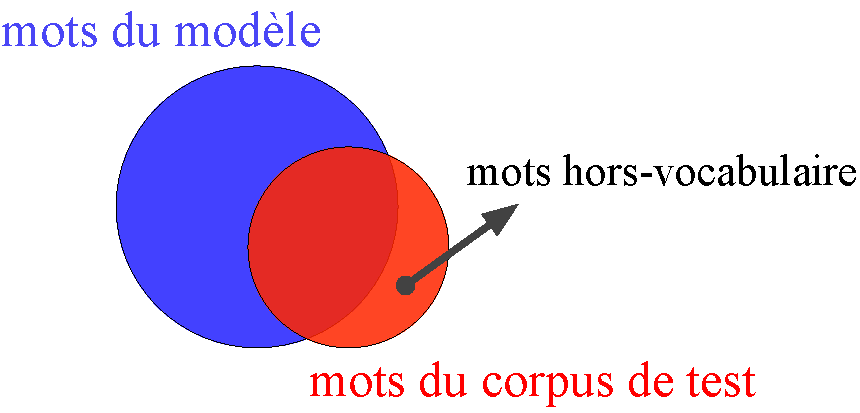
\includegraphics[scale=0.53]{images/pictures/vocabulary.pdf}
\caption{Mots hors-vocabulaire}
\label{Fig:OOVwords}
\end{figure}


Les mots hors-vocabulaire sont en fait les mots qui sont présents dans le corpus de test mais absents dans le vocabulaire du système de reconnaissance (cf. Fig. \ref{Fig:OOVwords}). 
Ces mots ne peuvent jamais être reconnus tels quels par le système de reconnaissance de la parole et sont remplacés par d'autres unités lexicales en fonction des modèles de reconnaissance. 
Dans le cas d'un modèle de langage grand vocabulaire, les mots hors-vocabulaire sont le plus souvent remplacés par une suite des petits mots ayant une prononciation similaire. 

%Pour les modèles de langage hybrides (mots et sous-mots), les mots hors-vocabulaire sont le plus souvent remplacés par des sous-mots. 


Les résultats reportés par la suite sont obtenus sur l'ensemble de développement du corpus ESTER2 qui contient 6517 mots différents avec 41374 occurrences (d'après les fichiers \acrshort{STM}).

\begin{table}[h!]
\centering
\begin{tabular}{|l|R{3.5cm}|R{3.5cm}|}
\hline
\textbf{Vocabulaire}	& \textbf{\# mots hors-vocabulaire} & \textbf{\% occ. mots hors-vocabulaire}	  \\ \hline
min3occ 		& 929 	& 4.34 \%	\\ \hline
min5occ 		& 1166	& 5.11 \%	\\ \hline
min25occ 		& 2452	& 9.51 \%	\\ \hline
min100occ 		& 4125	& 16.98	\%	\\ \hline
min300occ 		& 5369 	& 26.04	\%	\\ \hline
\end{tabular}
\caption{Nombre de mots hors-vocabulaire différents, et pourcentage d'occurrences}
\label{Tab:tauxOOV}
\end{table}

La liste des mots hors vocabulaire corresponde aux mots absents dans le lexique, mais présents dans la transcription. 
Le pourcentage d'occurrences est calculée par rapport à tous les mots du corpus évalué (41K mots).
Le nombre et le pourcentage d'occurrences des mots hors-vocabulaire relatifs aux différents lexiques hybrides sont affichés dans le tableau \ref{Tab:tauxOOV}~: ce taux augmente évidement lorsque la taille du lexique diminue.

\begin{figure}[h!]
\centering
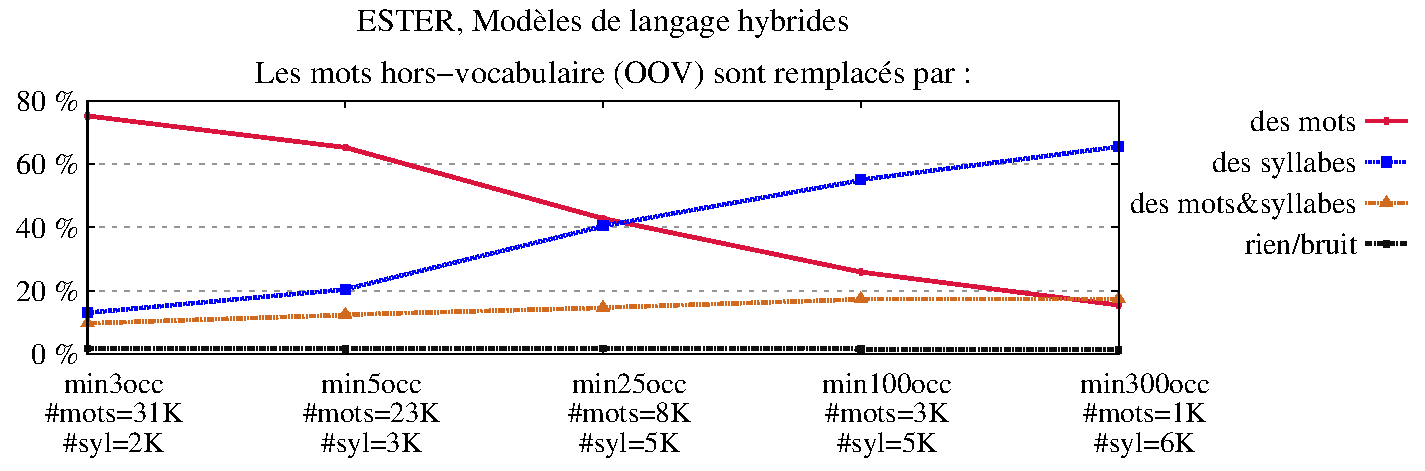
\includegraphics[scale=0.62]{images/results/ESTER_OOV_sv.pdf}
\caption{Analyse du décodage des mots hors vocabulaire sur le corpus ESTER2}
\label{Fig:OOV-ESTER}
\end{figure}


La figure \ref{Fig:OOV-ESTER} présente une analyse du décodage des mots hors vocabulaire par les modèles hybrides. 
Pour réaliser cette analyse nous avons identifié dans la transcription de référence les mots absents dans le vocabulaire du système de reconnaissance et nous avons récupéré la séquence correspondante d'unités lexicales dans chaque transcription automatique. L'analyse des résultats montre que les mots hors vocabulaire ont été remplacés par un ou plusieurs mots (courbe rouge), par une ou plusieurs syllabes (courbe rouge) ou par un mélange de mots et de syllabes (courbe orange); il arrive également que le décodeur reconnaisse cette zone de parole hors-vocabulaire par un segment de silence ou de bruit (courbe grise foncé). 
Les mots hors-vocabulaire ont été remplacés par des mots (1 ou plusieurs), par des syllabes ou par une séquence de mots et de syllabes. 
Dans le cas du plus grand modèle (`min3occ'), la plupart de mots hors-vocabulaire sont remplacés par d'autres mots (75\%). 
Ce taux diminue avec l'augmentation  du nombre de syllabes dans le lexique hybride, et les mots hors-vocabulaire sont de plus en plus fréquemment remplacés par des syllabes. 




%%%%%%%%%%%%%%%%%%%%%%%%%%%%%%%%%%%%%%%%%%%%%%%%
\hiddensubsection{Mesures de confiance}

Le logiciel de reconnaissance fournit une mesure de confiance pour chaque élément reconnu (mot ou syllabe). 
Avec PocketSphinx, cette mesure repose sur le calcul d'une probabilité a posteriori. 
Les mesures de confiance donnent une indication de la pertinence de la reconnaissance. Typiquement, les items ayant une mesure de confiance élevée sont généralement ``corrects'', et ceux ayant une mesure de confiance faible correspondent fréquemment à une erreur de reconnaissance. Il est ainsi possible en choisissant un seuil sur les mesures de confiance de traiter différemment les items ayant une mesure de confiance supérieure à ce seuil de ceux ayant une mesure de confiance inférieure à ce seuil.

Des tests subjectifs ont montré une préférence pour l'affichage sous forme phonétique des mots ayant une faible mesures de confiance \cite{Razik:2008}.

Notre approche est donc de conserver les mots avec une bonne probabilité d'être corrects (pour maximiser la bonne compréhension du message), et de remplacer les autres par des suites de phonèmes ou de syllabes \cite{Piquard:2015}. Le choix du seuil est donc crucial : un compromis doit être fait entre le nombre de mots qui sont rejetés (remplacés avec d'autres unités), et la performance obtenue sur les mots conservés. 


\begin{figure}[h!]
\begin{subfigure}{0.5\textwidth}
\centering
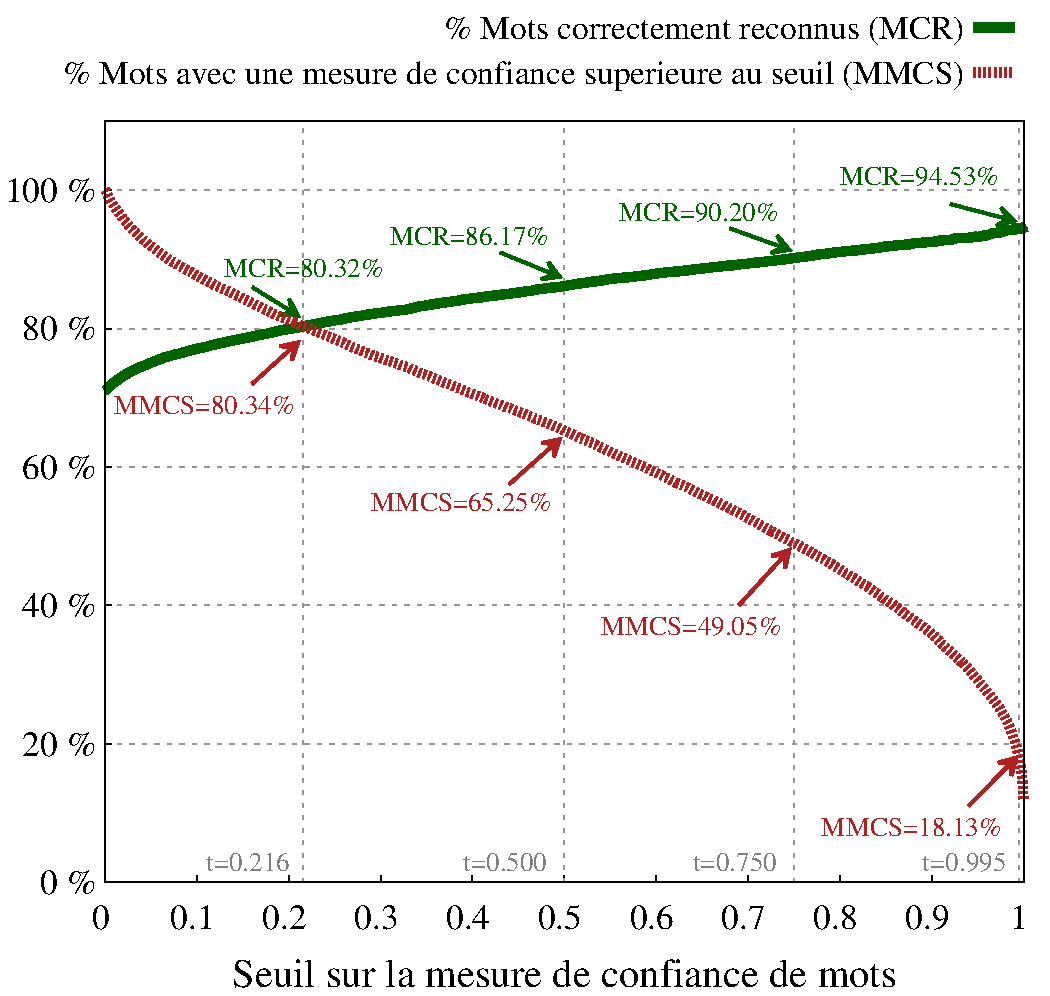
\includegraphics[scale=0.41]{images/results/ESTER_combined_min3occ_words_CM.pdf}
\caption{ML='min3occ'}
\end{subfigure}
\begin{subfigure}{0.5\textwidth}
\centering
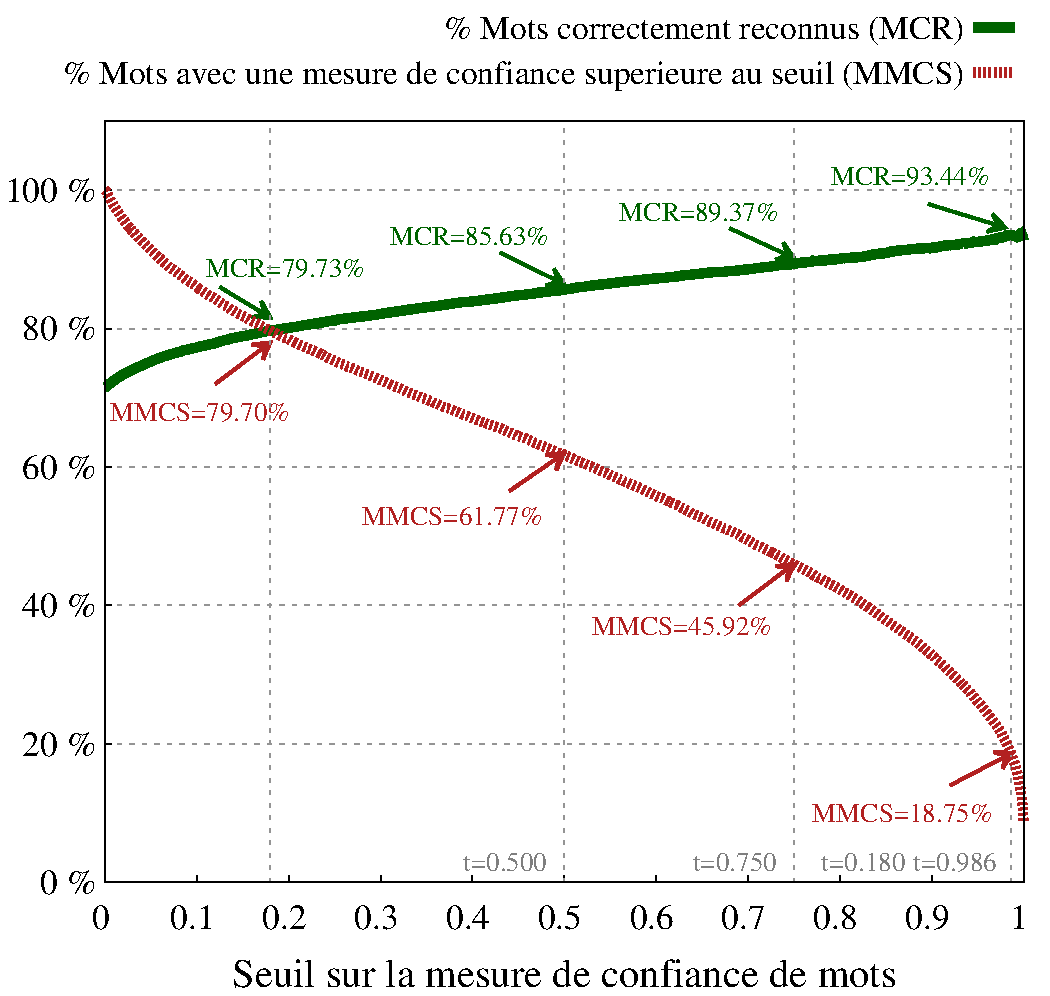
\includegraphics[scale=0.41]{images/results/ESTER_combined_min300occ_words_CM.pdf}
\caption{ML='min300occ'}
\end{subfigure}
\caption{Impact du choix du seuil sur la mesure de confiance de mots, pour les modèle de langage hybrides `min3occ' (a), et `min300occ' (b), sur le corpus ESTER2}
\label{Fig:MC-mots-ESTER2}
\end{figure}


La figure \ref{Fig:MC-mots-ESTER2} analyse les résultats sur les mots en fonction du choix du seuil sur les mesures de confiance, en utilisant le modèle de langage `min3occ' (a) et `min300occ' (b). 
La courbe verte (en trait plein, MCR) indique le pourcentage de mots correctement reconnus parmi ceux ayant une mesure de confiance supérieure au seuil choisi (axe horizontal). 
La courbe rouge (en pointillés, MMCS)  donne le pourcentage de mots qui ont une mesure de confiance supérieure à ce seuil. 
Bien évidemment, plus le seuil choisi sur la mesure de confiance est élevé, plus y a de réponses correctes parmi les items ayant une mesure de confiance supérieure à ce seuil ; malheureusement le nombre d'items ayant une mesure de confiance supérieure au seuil diminue. 
Les mesures de confiance calculées sur les mots sont pertinentes : environ 65\% de mots ont une mesure de confiance supérieure à 0,5 avec le modèle de langage `min3occ' et  environ 62\% avec le modèle de langage `min300occ'. 

Les résultats sur les syllabes en fonction du choix du seuil sur les mesures de confiance sont également étudiés (cf. Fig. \ref{Fig:MC-syllabes-ESTER2}).
La courbe verte (en trait plein, SCR) indique le pourcentage de syllabes correctement reconnues parmi celles ayant une mesure de confiance supérieure au seuil choisi (axe horizontal). 
La courbe rouge (en pointillés, SMCS) donne le pourcentage de syllabes qui ont une mesure de confiance supérieure à ce seuil. 
Avec le modèle 'min3occ' le taux de syllabes ayant une mesure de confiance supérieure à 0,5 est inférieur à 20\%, et le taux de syllabes correctement reconnues varie entre 50\% et 76\%.  
Les résultats obtenus avec le modèle 'min300occ' sont meilleurs : le taux de syllabes ayant une mesure de confiance supérieure à 0,5 est supérieur à 50\% et le taux de syllabes correctement reconnues varie entre 80\% et 96\%. 
Les mesures de confiance calculées sur les syllabes sont pertinentes seulement s'il existe une quantité relativement importante de syllabes dans le corpus d'apprentissage. 

\begin{figure}[h!]
\begin{subfigure}{0.5\textwidth}
\centering
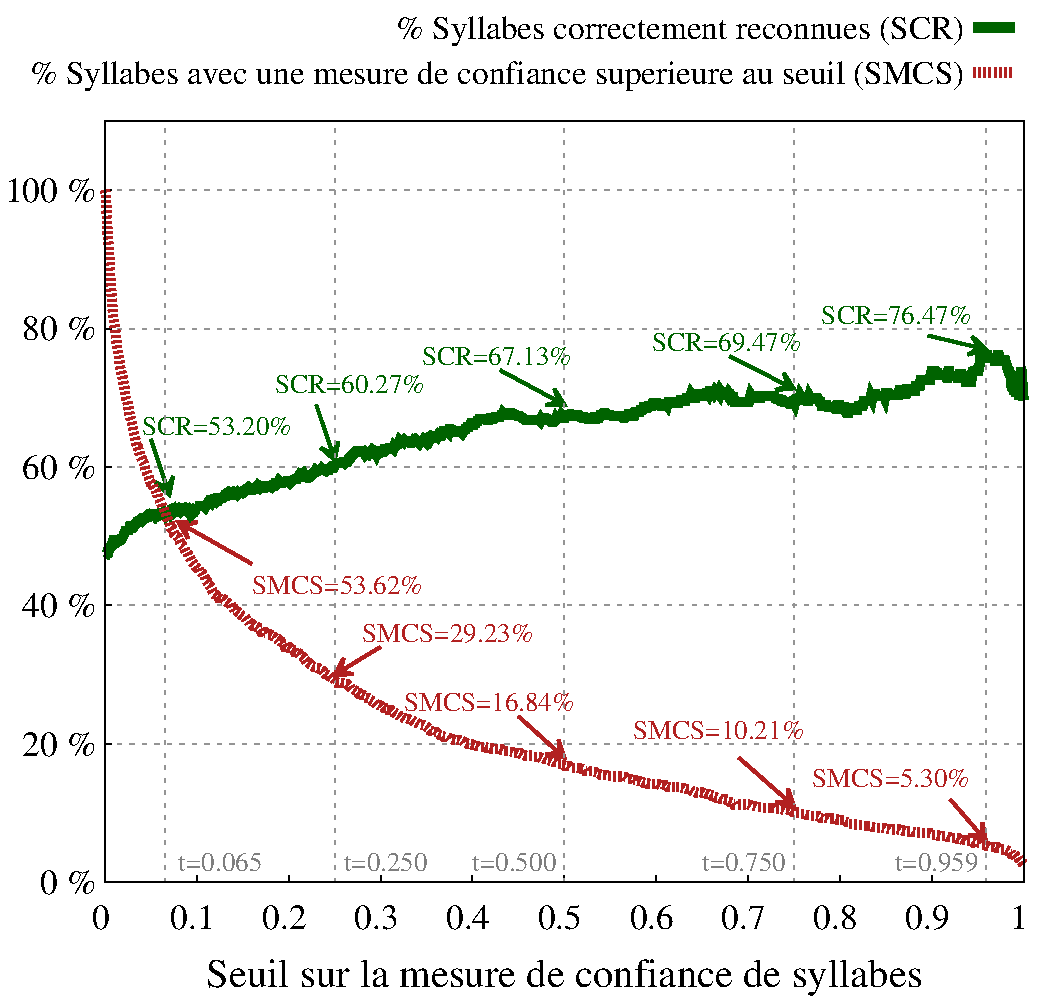
\includegraphics[scale=0.41]{images/results/ESTER_combined_min3occ_syllables_CM.pdf}
\caption{ML='min3occ'}
\end{subfigure}
\begin{subfigure}{0.5\textwidth}
\centering
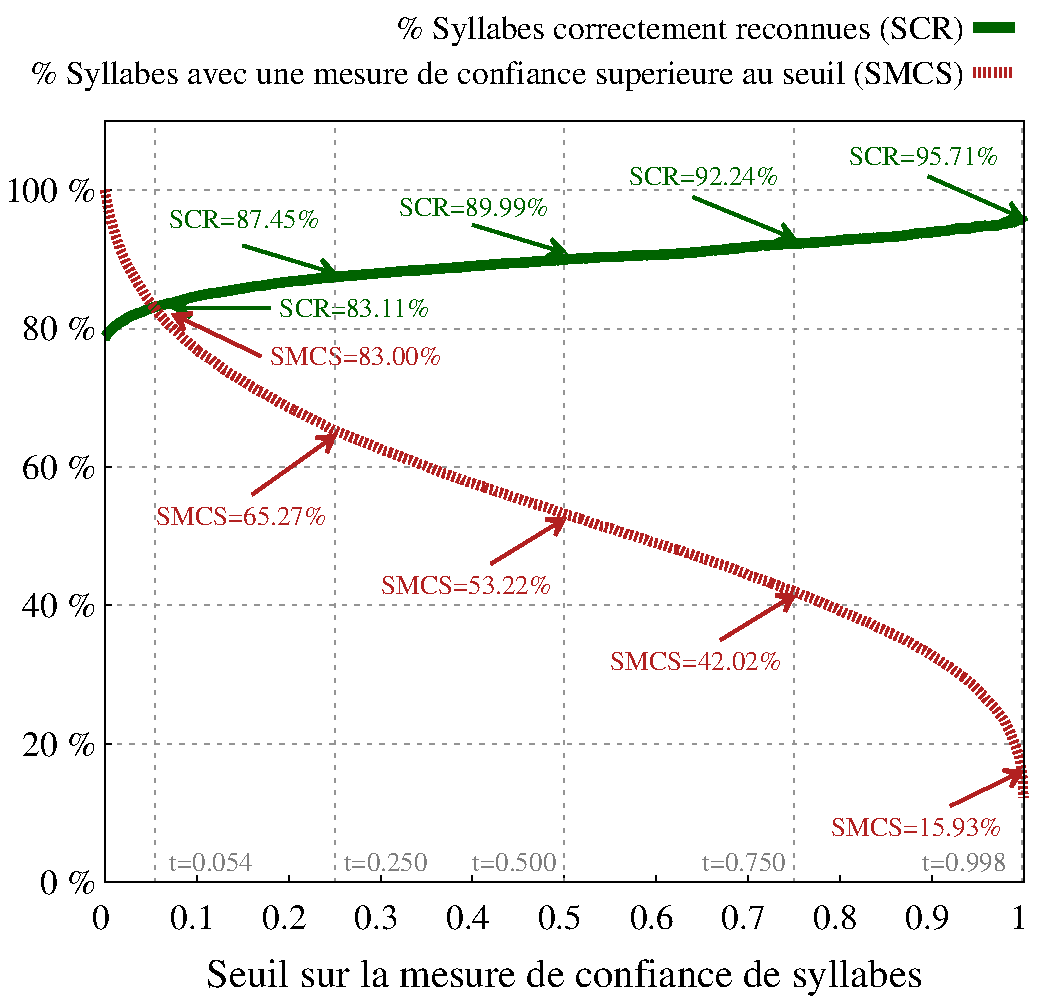
\includegraphics[scale=0.41]{images/results/ESTER_combined_min300occ_syllables_CM.pdf}
\caption{ML='min300occ'}
\end{subfigure}
\caption{Impact du choix du seuil sur la mesure de confiance des syllabes pour les modèles de langage hybrides `min3occ' (a) et `min300occ' (b) sur le corpus ESTER2}
\label{Fig:MC-syllabes-ESTER2}
\end{figure}

Les tests effectués ont montré un réel intérêt dans cette mesure. 
Cependant, plus de tests sur la version finale du produit permettront d'optimiser, par la suite, le choix du seuil. 

%===================================================================================
\section{Interpolation des modèles hybrides}
\renewcommand{\rightmark}{Interpolation des modèles hybrides}
%===================================================================================


Pour mieux modéliser les syllabes à l'intérieur d'un modèle hybride nous proposons de combiner deux modèles de langage hybrides, l'un offrant une bonne couverture des mots et l'autre une bonne couverture des syllabes. 
Le but est d'assurer une bonne reconnaissance d'un nombre important de mots, tout en améliorant les performances des syllabes pour la reconnaissance des mots hors-vocabulaire. 

L'interpolation entre deux modèles de langage hybrides implique un regroupement de leurs n-grammes et une mise-à-jour de leurs probabilités (cf. eq. \ref{Eq:mixLM}). 
En fonction d'une valeur $\lambda \in ]0,1[$, les probabilités n-grammes d'un modèle vont être privilégiées par rapport à l'autre~: un $\lambda$ se rapprochant de la valeur 1 va créer un modèle qui se rapproche des probabilités du premier modèle, et vice-versa — un $\lambda$ se rapprochant de la valeur 0 va créer un modèle qui se rapproche des probabilités du deuxième modèle.

\begin{equation}
\text{ML}_{mix} = \lambda \text{ML}_1 + (1-\lambda) \text{ML}_2
\label{Eq:mixLM}
\end{equation}

Nous avons analysé l'interpolation entre un modèle de langage qui contient une quantité importante de mots et quelques syllabes (`min3occ' - 31 000 mots et 2 000 syllabes) et un autre modèle qui contient une quantité importante de syllabes et quelques mots (`min300occ' - 1 000 mots et 6 000 syllabes), avec les valeurs $\lambda \in \{0,9; 0,8; 0,7; 0,6; 0,5;$ $0,4; 0,3; 0,2; 0,1\}$. Les modèles interpolés contiennent 31~000 mots et 6 000 syllabes.  

Les modèles interpolés sont comparés aux deux modèles de référence en ce qui \linebreak concerne les taux d'erreur, les taux de mots reconnus, taux de mots bien reconnus, les taux de mots hors-vocabulaire reconnus pas des syllabes, et la pertinence de mesures de confiance sur les syllabes.

Les figures suivantes affichent les différents résultats obtenus avec les modèles interpolés ($\lambda \in \{0,9; ...; 0,1\}$) sur les corpus de parole ESTER2 et ETAPE, en les comparant aux deux modèles de référence - le modèle `min3occ' (à gauche, équivalent à $\lambda=1$) et le modèle `min300occ' (à droite, équivalent à $\lambda=0$).

\begin{figure}[h!]
\centering
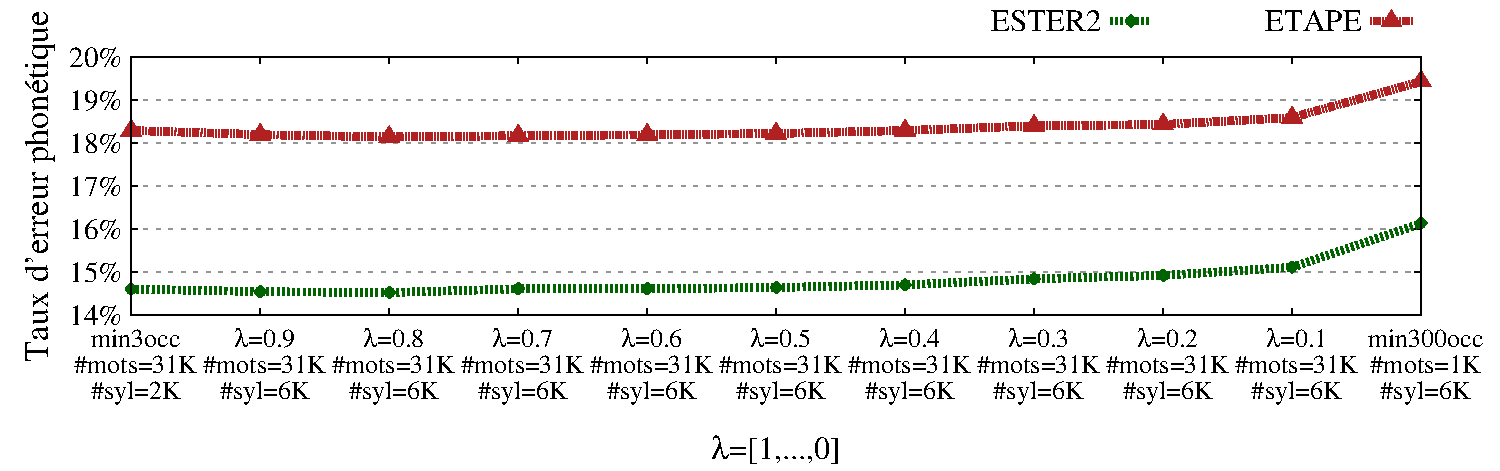
\includegraphics[scale=0.6]{images/results/results_PER_mixedLMs-3-300.pdf}
\caption{Taux d'erreur phonétique obtenus avec l'interpolation de deux modèles de langage hybrides `min3occ' et `min300occ'}
\label{Fig:PER-iLM}
\end{figure}

Les taux d'erreur phonétique des différents modèles sont présentés dans la figure \ref{Fig:PER-iLM} : les modèles interpolés produisent un taux d'erreur phonétique similaire à celui du premier modèle; les modèles $\lambda \in \{0,3; 0,2; 0,1\}$ présentent une dégradation non-significative. 

Les taux de mots produits par le décodeur dans les suites de mots et de syllabes,  les taux de mots correctement reconnus et les taux de syllabes correctement reconnues sont présentés dans la figure \ref{Fig:statsWS-mix}. 
Le taux de mots produits par le décodeur varie entre 95\% et 80\%, soit un écart d'environ 20\% de mieux en comparaison du taux produit par le modèle hybride `min300occ'.
Le taux de mots correctement reconnus avec les modèles interpolés est supérieur aux taux obtenus avec les modèles de référence~: environ 75\% pour le corpus ESTER2 et environ 72\% pour le corpus ETAPE. 
Le taux de syllabes correctement reconnues s'améliore pour les modèles qui s'approchent des probabilités n-grammes du deuxième modèle ($\lambda$ inférieur à 0,5) : il varie entre 47\% et 70\% avec un écart de 10\% par rapport aux taux obtenus avec le modèle `min300occ'.  


\begin{figure}[h!]
\centering
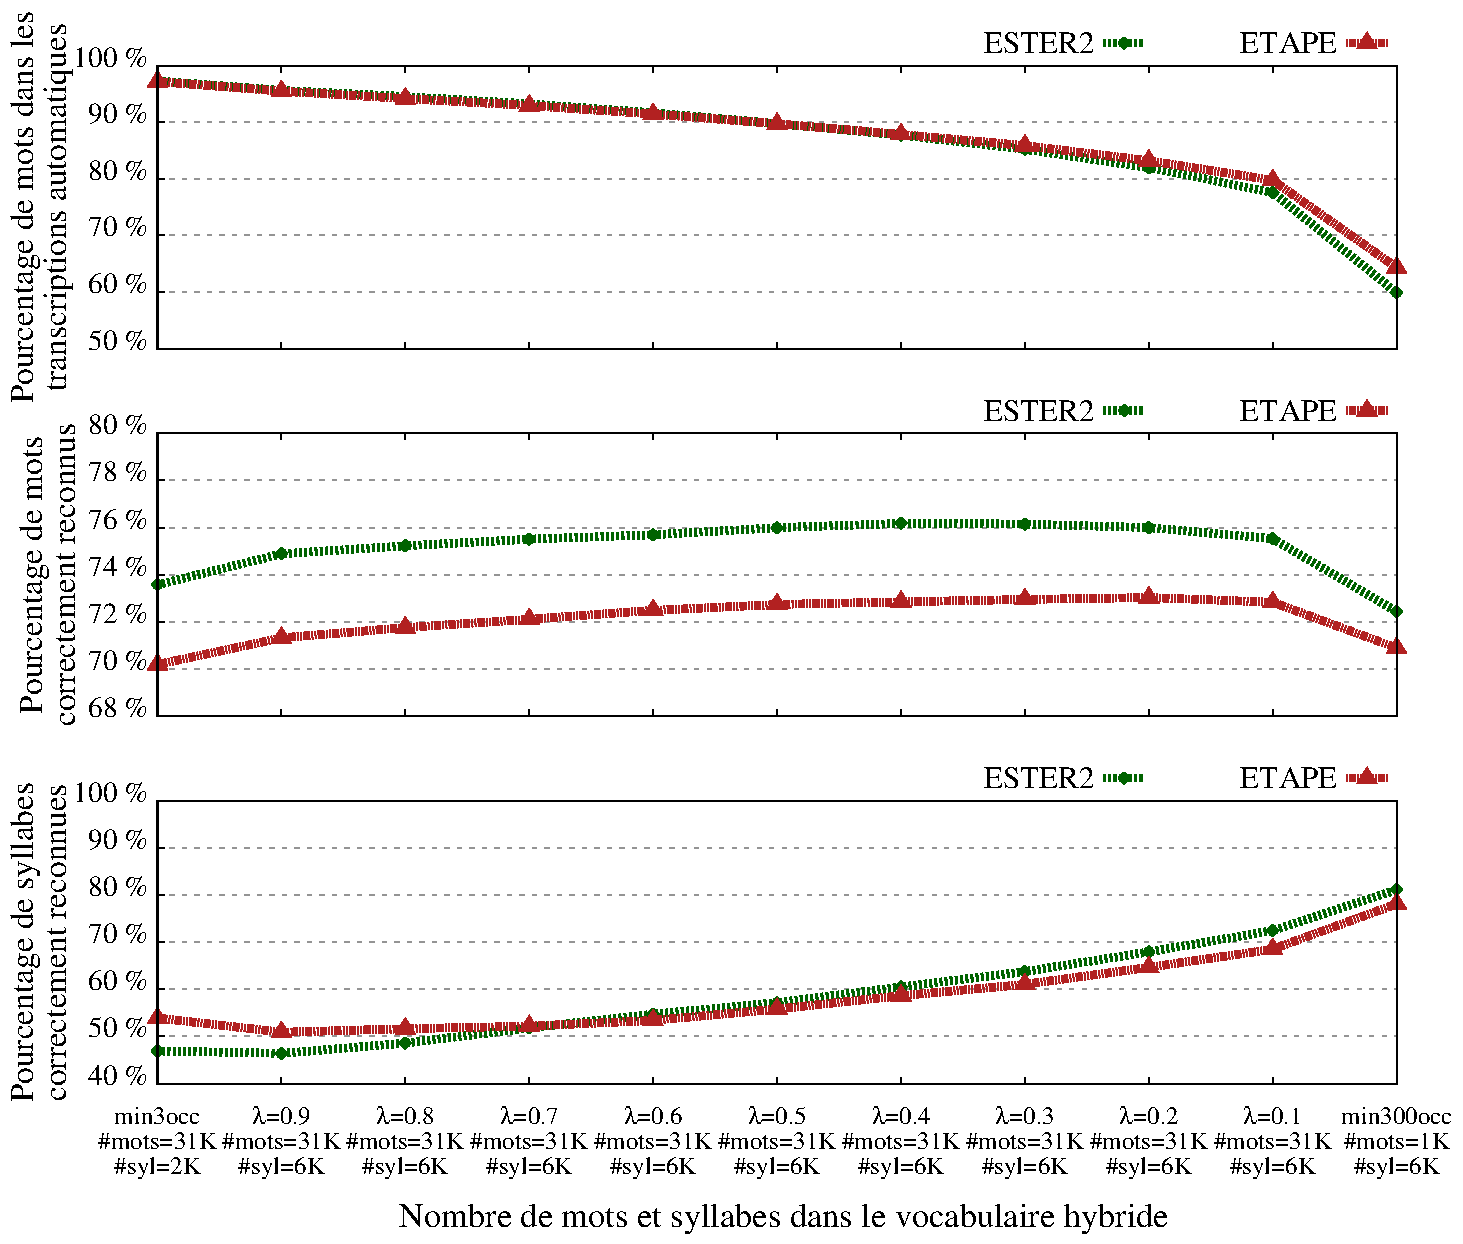
\includegraphics[scale=0.59]{images/results/statsWS_mixedLMs-3-300}
\caption{Taux de mots reconnus, de mots correctement reconnus et de syllabes correctement reconnues avec l'interpolation de deux modèles de langage hybrides `min3occ' et `min300occ'}
\label{Fig:statsWS-mix}
\end{figure}

La figure \ref{Fig:OOV-ESTER-iLM} présente les résultats sur les mots hors-vocabulaire. 
Les modèles interpolés améliorent le taux de mots hors-vocabulaire reconnus par des syllabes (entre 18\% et 32\%), ce qui est bénéfique compte-tenu de l'affichage envisagé dans l'application. Cependant, il y a toujours un écart de 33\% avec le deuxième modèle `min300occ', qui remplace 65\% de mots hors-vocabulaire par des syllabes.


Ces analyses visent à déterminer la meilleure combinaison entre les deux modèles de langage hybrides qui permet de conserver les atouts du premier modèle (reconnaissance majoritaire de mots, bonne reconnaissance de mots, bonnes mesures de confiance sur les mots) et d'améliorer la performance des syllabes grâce au deuxième modèle.  
Une combinaison 40\%-60\% ($\lambda=0.4$) assure une reconnaissance majoritaire de mots (88\%), une bonne reconnaissance de mots connus par le système (76\% sur ESTER2 et 73\% sur ETAPE), une meilleure reconnaissance de syllabe (60\%) et elle double la quantité de mots hors-vocabulaire qui sont reconnus par des syllabes (27\% comparé au 13\%).

\begin{figure}[h!]
\centering
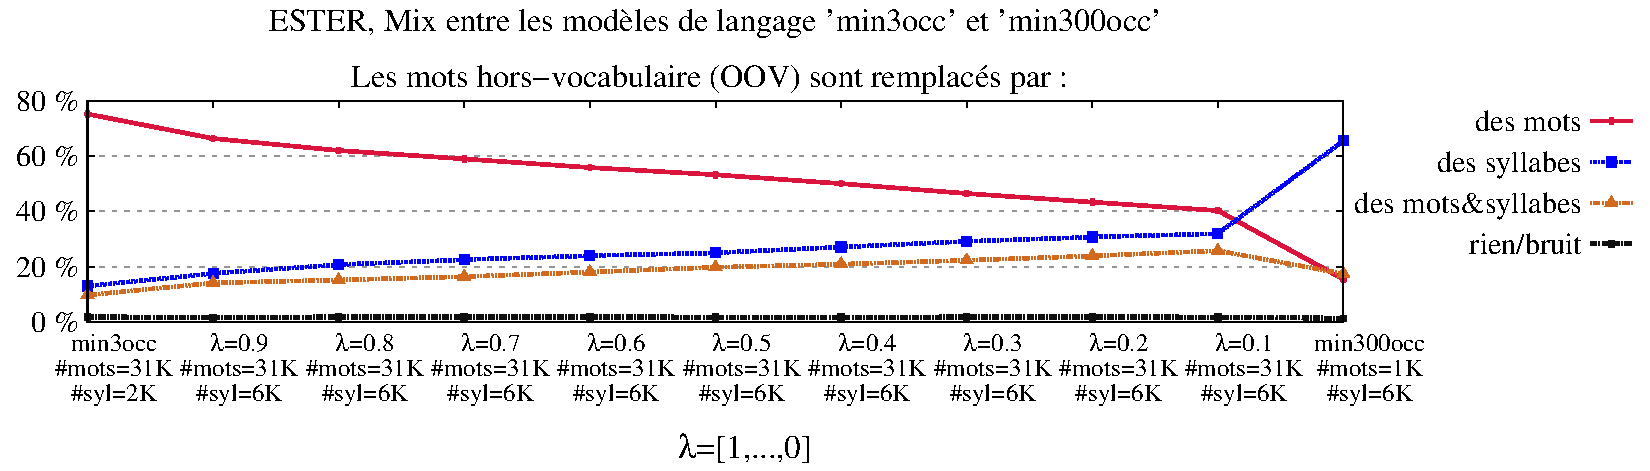
\includegraphics[scale=0.52]{images/results/ESTER_OOV_mixedLMs-3-300.pdf}
\caption{Analyse du décodage des mots hors-vocabulaire avec l'interpolation de deux modèles de langage hybrides `min3occ' et `min300occ' sur le corpus ESTER2}
\label{Fig:OOV-ESTER-iLM}
\end{figure}


 
Les résultats sur les sorties mots et syllabes, en fonction du choix du seuil sur les mesures de confiance, en utilisant le modèle de langage interpolé ($\lambda=0,4$) entre les modèles hybrides `min3occ' et `min300occ' sont affichés dans la figure \ref{Fig:MC-ESTER2-lambda04}. 
Les mesures de confiance sur les mots sont similaires à celles obtenues avec les modèles de langage `min3occ' et `min300occ'. 
Les mesures de confiance sur les syllabes ne sont toujours pas pertinentes : le taux de syllabes correctement reconnues varie entre 60\% et 73\% et seulement 21\% de syllabes ont une mesure de confiance supérieure à 0,5.



\begin{figure}[h!]
\begin{subfigure}{0.5\textwidth}
\centering
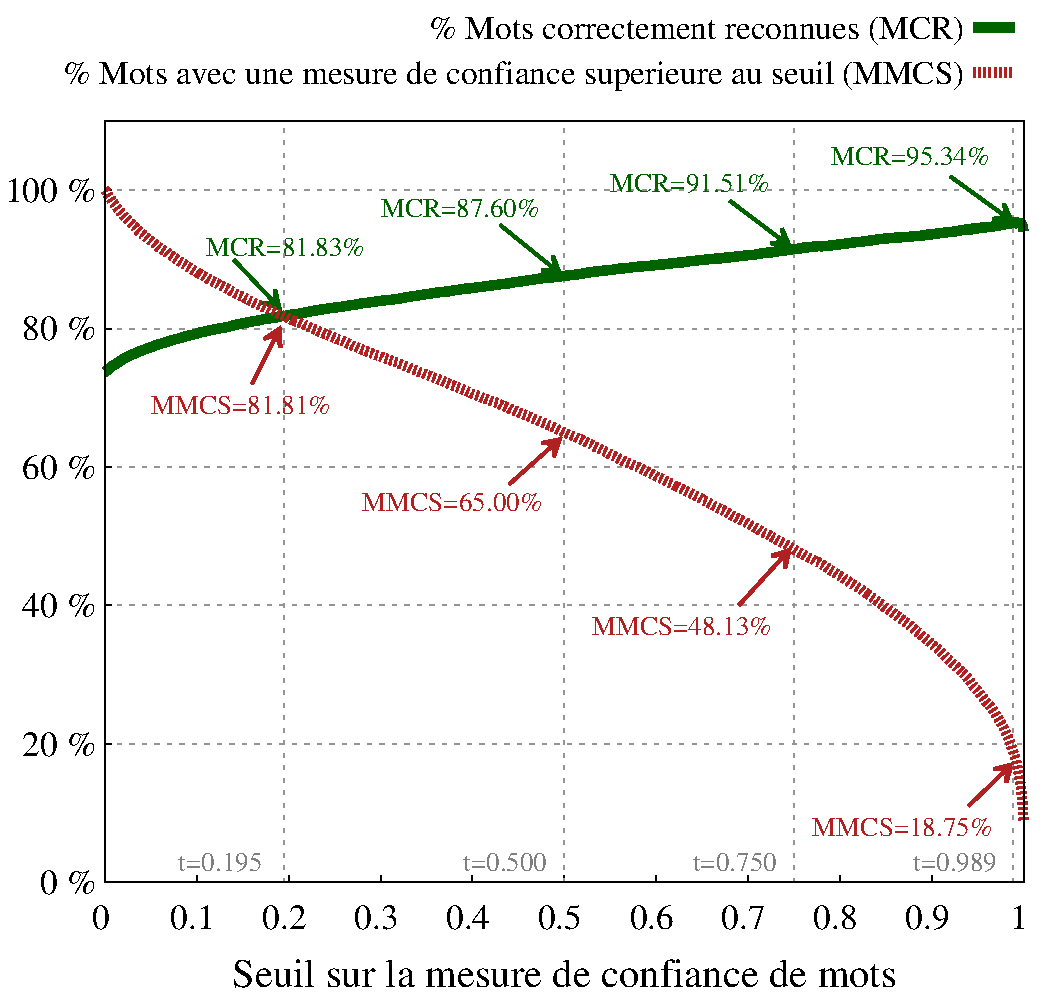
\includegraphics[scale=0.4]{images/results/ESTER_combined_mixedLMs-3-300-lambda40_words_CM.pdf}
\caption{Mots}
\end{subfigure}
\begin{subfigure}{0.5\textwidth}
\centering
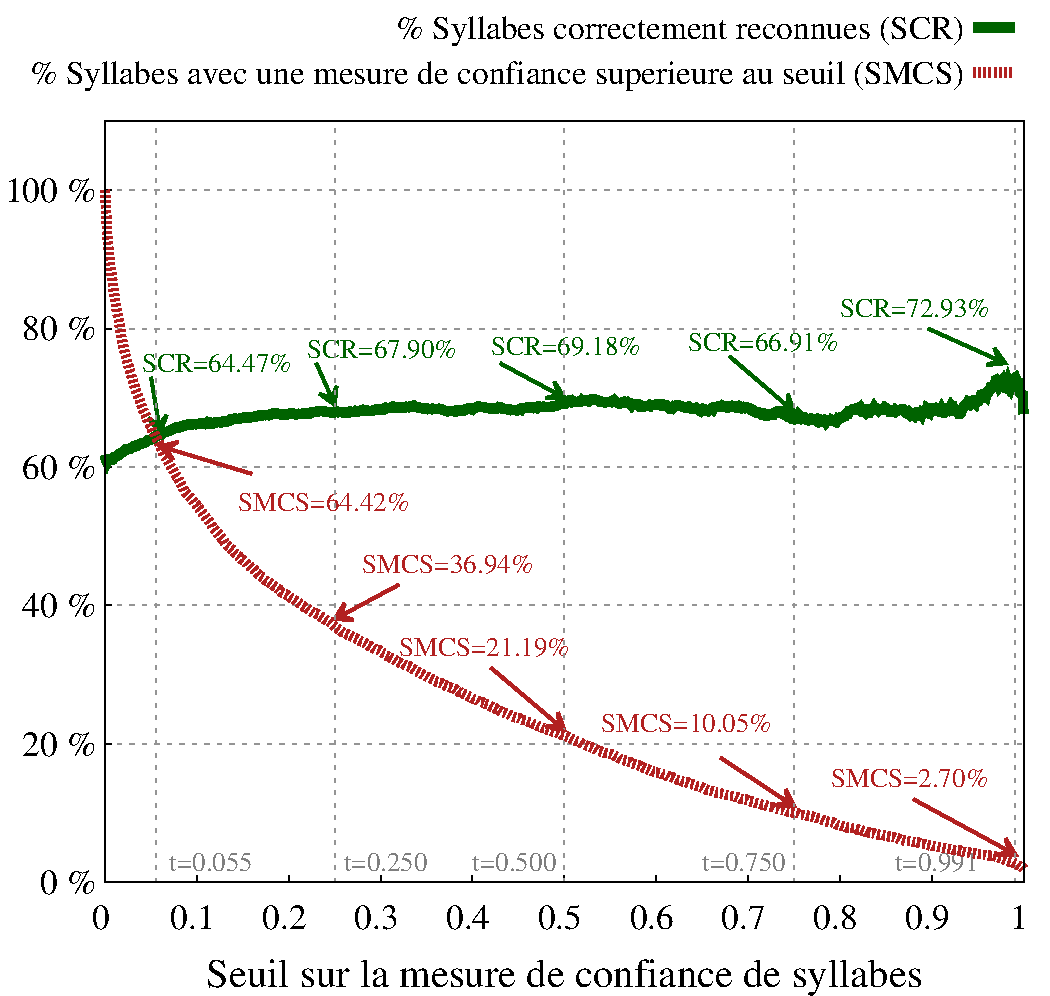
\includegraphics[scale=0.4]{images/results/ESTER_combined_mixedLMs-3-300-lambda40_syllables_CM.pdf}
\caption{Syllabes}
\end{subfigure}
\caption{Impact du choix du seuil sur la mesure de confiance de mots (a) et de syllabes (b) pour le modèle de langage interpolé $\lambda=0,4$ entre les modèles hybrides `min3occ' et `min300occ' sur le corpus ESTER2 }
\label{Fig:MC-ESTER2-lambda04}
\end{figure}



%%%%%%%%%%%%%%%%%%%%%%%%%%%%%%%%%%%%%%%%%%%%%%%%%%%%%%%%%%%%%%%%%%%%%%%%%%%%
\chapter{Ajout de nouveaux mots}
\renewcommand{\leftmark}{Ajout de nouveaux mots}
\renewcommand{\rightmark}{}
%%%%%%%%%%%%%%%%%%%%%%%%%%%%%%%%%%%%%%%%%%%%%%%%%%%%%%%%%%%%%%%%%%%%%%%%%%%%

Ce chapitre propose et évalue une nouvelle approche pour ajouter de nouveaux mots dans un modèle de langage. 
L'ajout de nouveaux mots est nécessaire dans le contexte du projet afin d'assurer une bonne reconnaissance des mots spécifiques à un certain domaine (par exemple mots utiles dans un magasin de bricolage, qui est le contexte applicatif choisi dans le projet pour la validation et l'expérimentation; et aussi pour pouvoir tenir compte de l'arrivée de nouveaux produits ou services).

L'approche proposée est basée sur un principe de similarité entre mots. 
Cette partie du travail est publiée dans un article de conférence \cite{Orosanu2015_2}. % et un article de workshop \cite{}.

\minitoc

%====================================================================
\section{Approche}
\renewcommand{\rightmark}{Approche}
%====================================================================

Pour ajouter de nouveaux mots dans un modèle de langage et faire face à l'impossibilité de trouver une quantité importante des données textuelles les représentant, nous avons proposé une nouvelle approche basée sur la similarité entre mots.

L'idée est de considérer que deux mots sont similaires s'ils ont les mêmes prédécesseurs et successeurs. 
Formellement, la comparaison (recherche de similarité) entre deux mots se traduit par un calcul de divergence entre les distributions des mots prédécesseurs et des mots successeurs. 
L'approche implique ainsi plusieurs étapes : utiliser quelques phrases exemples contenant le nouveau mot, chercher dans le modèle de langage des mots similaires au nouveau mot, puis définir les n-grammes associés au nouveau mot à partir des n-grammes des mots similaires. 


%%%%%%%%%%%%%%%%%%%%%%%%%%%
\hiddensubsection{Recherche des mots similaires}

Un ensemble de phrases est nécessaire afin de disposer d'un minimum d'information sur les nouveaux mots. 
Il peut être récupéré sur internet ou composé manuellement. 
Les voisins, prédécesseurs et successeurs, des nouveaux mots sont extraits de ces phrases, afin de calculer leurs distributions de probabilités.
Pour chaque nouveau mot $nW$ (\textit{new word}) on calcule la distribution de probabilités $P_k(w|nW)$ de tous les voisins $w$ trouvés dans chaque position $k$, avec $k \in \{..., -3, -2, -1, +1, +2, +3, ...\}$.

Un ensemble différent de données est utilisé pour représenter les mots ``connus'' (i.e. dans le vocabulaire) . 
Les compteurs 2-grammes  permettent de calculer les distributions de 2 voisins (-1, + 1), les compteurs 3-grammes permettent de calculer les distributions de 4 voisins (-2, -1, + 1, + 2), et ainsi de suite.
Les voisins prédécesseurs et successeurs de chaque mot ``connu'' sont extraits à partir des compteurs n-grammes, afin de calculer leurs distributions de probabilités.
Pour chaque mot connu $kW$ (\textit{known word}) on calcule la distribution de probabilités $P_k(w'|kW)$ de tous les voisins $w'$ trouvés dans chaque position $k$, avec $k \in \{..., -3, -2, -1, +1, +2, +3, ...\}$.

La (dis)similarité entre les distributions de voisins $w$ d'un nouveau mot $nW$ et d'un mot connu $kW$ est évaluée par la divergence KL \cite{Kullback:1951} sur chaque position $k$ :


\begin{equation}
\begin{split}
D_{k}(kW,nW) =& D_{KL} \left(P_k(\bullet|kW)\ ||\ P_k(\bullet|nW)\right) \\
			=& \sum_w P_k(w|kW)\ log \frac{P_k(w|kW)}{P_k(w|nW)}
\end{split}
\end{equation}

La divergence KL est calculée sur les voisins $w$ des nouveaux mots pour chaque position $k$. Si ces voisins ne sont pas présents dans la liste des voisins d'un mot connu, leur probabilité est remplacée avec une petite valeur $\lambda$  par défaut  (dans nos expériences $\lambda = 1e^{-7}$).

La (dis)similarité globale entre deux mots est définie comme la somme des divergences sur toutes les $k$ positions de voisins (cf. eq. \ref{Eq:DivT}).
Les mots les plus similaires avec un nouveau mot sont ceux ayant les divergences les plus faibles.

\begin{equation}
D(kW,nW) = \sum_k D_k(kW,nW)
\label{Eq:DivT}
\end{equation}


%%%%%%%%%%%%%%%%%%%%%%%%%%%
\hiddensubsection{Ajout de nouveaux n-grammes}

L'algorithme suivant décrit notre méthode d'ajout de n-grammes correspondants à un nouveau mot dans un modèle de langage. 

Le nouveau modèle de langage (\textit{newLM}) est initialisé avec tous les n-grammes du modèle baseline. 
Chaque entrée n-gramme (\textit{ngram}) du modèle baseline est analysée pour vérifier si elle contient un mot connu (\textit{kW}) qui fait partie de la liste de mots similaires du nouveau mot à ajouter (\textit{similarWords(nW)}). 
Si c'est le cas, une nouvelle entrée n-gramme est créée en remplaçant le mot connu (\textit{kW}) avec le nouveau mot (\textit{nW}) qui lui est similaire, et cette nouvelle entrée n-gramme est ensuite ajoutée dans le nouveau modèle de langage. 
À noter que le remplacement des mots connus par le nouveau mot (avec lequel il y a similarité) peut produire plusieurs n-grammes ayant la même séquence de mots mais avec des probabilités différentes. 
Dans ces cas, une seule entrée est conservée pour la séquence de mots correspondante, avec la valeur médiane de probabilité.


\begin{algorithm}[h!]
\caption{\textbf{Algorithme} Ajouter des nouveaux n-grammes dans le modèle de langage}
\label{Alg:AddNewWords}
\begin{algorithmic}[1]
\Procedure{addNgrams}{\textbf{\color{red}n}}
\State {\color{blue}newLM} $\leftarrow$ LM
\State {\color{blue}newNgrams} $\leftarrow$ $\varnothing$
\BState \emph{\color{gray}\# traiter les n-grams du modèle baseline}
\For {\textbf{each} \textbf{\color{red}n}gram $\in$ LM}
	\For {\textbf{each} kW $\in$ similarWords(nW)}
		\If {$contains$(\textbf{\color{red}n}gram, kW)}		
		\State \textbf{\color{red}n}gram\textbf{'} $\leftarrow$ $replace$(\textbf{\color{red}n}gram, kW, nW)
		\State push({\color{blue}newNgrams}, \textbf{\color{red}n}gram\textbf{'})
		\EndIf
	\EndFor
\EndFor

\BState \emph{\color{gray}\# choisir les nouveaux n-grams à ajouter dans le nouveau modèle}
\State S  $\leftarrow$ $getUniqueSequences$({\color{blue}newNgrams})
\For {\textbf{each} seq $\in$ S}
	\If {$frequency$(seq) = 1}
		\State prob  $\leftarrow$ $getProbability$(seq)
	\Else
		\State P  $\leftarrow$ $getProbabilities$(seq)
		\State prob $\leftarrow$ $medianProbability$(P)
	\EndIf
	\State push({\color{blue}newLM},  ''seq prob'')
\EndFor
\EndProcedure
\end{algorithmic}
\end{algorithm}


%Par exemple, un appel de la procédure ``addNgrams(1)'' ajoute les 1-grammes associés au nouveau mot dans le nouveau modèle de langage.

Les poids de back-off sont ensuite renormalisés.

\vskip-0.1ex

%====================================================================
\section{Expérimentations}
\renewcommand{\rightmark}{Expérimentations}
%====================================================================

Cette section présente les expérimentations menées pour évaluer l'approche proposée, et analyse les résultats.
Le contexte expérimental est décrit~: choix de nouveaux mots, choix des données textuelles exemples pour les nouveaux mots, nombre de mots similaires à conserver pour chaque nouveau mot et type des n-grammes à ajouter dans le nouveau modèle de langage. 
Les différents modèles de langage obtenus sont ensuite évalués sur l'ensemble de données de développement d'ESTER2. 

%=====================================================================
\hiddensubsection{Recherche de mots similaires}

Nous avons sélectionné une liste de 20 ``nouveaux'' mots, vus entre 50 et 100 fois dans les ensembles de développement d'ESTER2 et d'ETAPE :  \{soirée, place, gouvernement, moment, exemple, problème, pouvoir, tour, niveau, nombre, groupe, histoire, journal, sécurité, réunion, projet, année, guerre, jour, rapport\}.
Nous avons ajouté à cette liste leurs formes féminine, masculine et pluriel pour éviter que le décodeur choisisse une de ces formes comme remplacement à cause de leur prononciations similaires. La liste finale contient 44 mots. 
L'ensemble de ces mots a une fréquence d'occurrence de 1,33\% dans le corpus de développement d'ESTER2, et la suppression de ces mots du lexique et du modèle de langage conduit à une augmentation significative du taux d'erreur mot (26,97\% au lieu de 24,80\%).

Pour chaque nouveau mot, \{5, 10, 20, ou 50\} phrases exemples ont été extraites de manière aléatoire des corpus Wikipedia et GigaWord. 
Différentes distributions de probabilités ont été testées en utilisant \{2 voisins, 4 voisins ou 6 voisins\}.

Pour donner un exemple avec 6 voisins, dans la phrase ``les précipitations sont également \underline{réparties} \underline{sur} \underline{l'} \textbf{année} \underline{avec} \underline{un} \underline{total} de 610 millimètres de pluie'', le nouveau mot ``année'' a comme voisin en position -3 le mot `réparties', voisin en position -2 le mot `sur', ..., voisin en position +3 le mot `total'.

Le corpus Wikipedia est utilisé pour calculer les compteurs n-grammes des mots connus (par rapport à un vocabulaire de 97K mots ignorant les nouveaux mots). 

Pour le 4-gramme ``cèdent leur place à'' (qui a été vu 9 fois) le mot ``cèdent'' a comme voisin en position +1 le mot `leur', voisin en position  +2 le mot `place' et voisin en position +3 le mot `à'; le mot ``leur'' a comme voisin en position  -1 le mot `cèdent', voisin en position  +1 `place' et voisin en position +2 `à', ..., le mot ``à'' a comme voisin en position  -3 le mot `cèdent', et ainsi de suite.

Pour la recherche des mots similaires aux nouveaux mots, la prise en compte d'informations complémentaires a été étudiée en considérant la classe grammaticale et le lemme des mots. 
En conséquence, toutes les phrases ont été annotées avec les unités ``mot$|$\linebreak classeGrammaticale'' et ``lemme$|$classeGrammaticale'' correspondantes. 

Différentes listes de mots similaires sont obtenues selon que l'on considère les unités mots, les unités ``mot$|$classeGrammaticale'' ou les unités ``lemme$|$classeGrammaticale''. À noter que les unités ``lemme$|$classeGrammaticale'' ne peuvent pas être utilisés avec les formes féminine, masculine, pluriel des mots (puisque tous les mots sont réduits à la forme racine).

Voici un exemple de listes de 10 mots similaires obtenus pour le nouveau mot ``journal'' en considérant 10 phrases exemples et la distribution de 6 voisins (avec les fichiers de compteurs 4-grammes de Wikipedia) :
\begin{itemize}
\item basée sur les mots : \{nom, premier, jeux, livre, paire, monde, magasine, deuxième\}
\item basée sur les unités ``mot$|$classeGrammaticale'' : \{magasine, nom, titre, jeux, livre, monde, service, texte, programme, reseau\}
\item basée sur les unités ``lemme$|$classeGrammaticale'' : \{chronique, titre, magasine, nom, série, livre, version, gamme, programme, presse\}
\end{itemize}

Pour les expériences suivantes, les mots similaires sont obtenus avec la \linebreak distribution de 4 voisins en considérant les unités ``mot$|$classeGrammaticale''. 

Les tableaux \ref{Tab:SWords-5} et \ref{Tab:SWords-50} en annexe donnent les 5 mots les plus similaires obtenus pour chaque nouveau mot en considérant 5 et respectivement 50 phrases exemples (avec la distribution de 4 voisins en considérant les unités ``mot$|$classeGrammaticale'').


%=====================================================================
\hiddensubsection{Ajout de mots dans le modèle de langage}

Un modèle de langage grand vocabulaire (97K mots) a été appris sur données textuelles variées (1,3Md mots, 58M phrases), après suppression des phrases contenant les nouveaux mots. 
Il contient  97 305 1-grammes, 37,1M 2-grammes et 63,1M 3-grammes.
Ce modèle est le modèle `baseline'; les 44 nouveaux mots sont des mots hors-vocabulaire pour ce modèle. 

Pour l'évaluation de l'ajout des nouveaux mots au modèle `baseline', trois paramètres différents ont été testés dans nos expériences : ajouter seulement les 1-grammes (`+1-grammes'), les 1-grammes et 2-grammes (`+1-,2-grammes') ou tous les n-grammes (`+1-,2-,3-grammes) définis pour les 44 nouveaux mots (à partir des mots similaires).

Plusieurs listes de mots similaires ont été évaluées en utilisant \{5, 10, 20 ou 50\} phrases exemples pour chaque nouveau mot et en choisissant les premiers \{5, 10, 20 ou 50\} mots connus les plus similaires à chaque nouveau mot.

Pour chacune de ces situations, un nouveau modèle de langage a été fabriqué en ajoutant les 1-grammes associés aux nouveaux mots (`baseline+1-grammes'), un autre en ajoutant les 1-grammes et 2-grammes associés aux nouveaux mots (`baseline+1-,2-grammes') et un troisième en ajoutant les 1-grammes, 2-grammes et 3-grammes associés aux nouveaux mots (`baseline+1-,2-,3-grammes'). 

Le tableau \ref{Tab:AddedNgrams} indique le nombre de 2-grammes et de 3-grammes associés aux modèles de langage `baseline+1-,2-,3-grammes'. 
L'utilisation de 5 phrases exemples et de 5 mots similaires pour chaque nouveau mot génère le plus petit nouveau modèle (`baseline\linebreak+1-,2-,3-grammes-5ex-5mS') qui ajoute 2\% de nouveaux 2-grammes et 6\% de nouveaux 3-grammes (en comparaison avec le modèle `baseline'). L'utilisation de 50 phrases \linebreak exemples et de 50 mots similaires pour chaque nouveau mot génère le plus grand nouveau modèle (`baseline+1-,2-,3-grammes-50ex-50mS') qui ajoute 10\% de nouveaux 2-grammes et 49\% de nouveaux 3-grammes.
%Entre 1 à 4 millions de 2-grammes et entre 4 à 31 millions de 3-grammes sont ajouté dans les nouveaux modèles de langage, en comparaison avec le modèle `baseline'. 

\begin{table}[h!]
\centering
\begin{tabular}{|r|r|r|r|r|}
\cline{2-5}
\multicolumn{1}{c|}{} 	& 5 mS	& 10 mS	& 20 mS	& 50 mS		\\ \hline
5 ex 			& 38,0 	& 38,6	& 39,2	& 40,3		\\ \hline
10 ex  			& 38,1 	& 38,6	& 39,3	& 40,5		\\ \hline
20 ex			& 38,2	& 38,7	& 39,4	& 40,6		\\ \hline
50 ex			& 38,1	& 38,7	& 39,5	& 40,7		\\ \hline
\end{tabular}
\hspace{0.1cm}
\centering
\begin{tabular}{|r|r|r|r|r|}
\cline{2-5}
\multicolumn{1}{c|}{}  	& 5 mS	& 10 mS	& 20 mS	& 50 mS		\\ \hline
5 ex 			& 67,2	& 71,7	& 76,0	& 86,7		\\ \hline
10 ex  			& 68,1	& 71,4	& 77,4	& 89,8		\\ \hline
20 ex			& 68,5	& 72,1	& 77,9	& 93,2		\\ \hline
50 ex			& 68,4	& 72,3	& 79,4	& 94,2		\\ \hline
\end{tabular}

\vskip1ex 
\begin{tabular}{p{7cm}p{7cm}}
\centerline{(a) \#2-grammes}\medskip & \centerline{(b) \#3-grammes}	\\
\end{tabular}
\vskip-0.6cm
\caption{Nombre de 2-grammes (a) et de 3-grammes (b) [en millions] dans les nouveaux modèles de langage `baseline+1-,2-,3-grammes', en fonction du nombre de phrases exemples par nouveau mot (\textit{ex}) et du nombre de mots similaires \\pour chaque nouveau mot (\textit{mS})}
\label{Tab:AddedNgrams}
\end{table}

Les modèles `baseline+1-,2-grammes' ont le même nombre de 2-grammes que les modèles `baseline+1-,2-,3-grammes'. 
Dans tous les cas, le nombre de 1-grammes passe de 97305 à 97349 par rapport au modèle `baseline'. 


%\vskip-0.2cm

%=====================================================================
\hiddensubsection{Modèles de langage de référence}

Un modèle ORACLE est fabriqué pour établir la performance maximale que l'on peut atteindre lorsque les nouveaux mots sont déjà connus et le modèle de langage correspondant correctement appris.
Ce modèle est appris sur les mêmes données que le modèle `baseline', mais sans supprimer les phrases associées aux nouveaux mots (1,7Md mots, 74M phrases). 
Les 44 ``nouveaux mots'' font partie de son vocabulaire. 

Pour rappel, compte tenu des différentes sources de données et des différentes tailles de données, les modèles de langage `baseline' et ORACLE sont fabriqués par interpolation; les poids optimaux d'interpolation sont estimés sur l'ensemble de données de développement d'ETAPE.

Quatre modèles de langage supplémentaires (LM-INTERP-1, LM-INTERP-2, LM-INTERP-3 et LM-INTERP-4) ont été utilisés pour valider notre approche d'ajout de nouveaux mots.
Ils ont été appris sur les mêmes ensembles de données que le modèle `baseline', plus un autre (petit) ensemble de données contenant les \{5, 10, 20 ou 50\} phrases exemples pour chaque nouveau mot. Les poids optimaux d'interpolation sont estimés également sur le corpus de développement d'Etape : les poids associés aux modèles de langage appris sur \{5, 10, 20 ou 50\} phrases exemples pour chaque nouveau mot sont respectivement de \{4.73\%, 5.06\%, 5.30\%, 5.71\%\}. 
Les 44 nouveaux mots ont une fréquence d'occurrence de 0.93\% dans le corpus de développement d'Etape.

Le tableau \ref{Tab:am-LMs} indique les tailles des modèles de langage utilisés comme référence dans nos expériences.

\begin{table}[h!]
\centering
\begin{tabular}{|l|r|r|r|}
\hline
\textbf{LM}  		& \textbf{1-grammes} 		& \textbf{2-grammes} 		& \textbf{3-grammes} 		\\ \hline
baseline		& 97 305  			& 37,1M   			& 63,1M				\\ \hline
modèles interpolés 	& \multirow{2}{*}{97 349}	& \multirow{2}{*}{37,1M}	& \multirow{2}{*}{63,1M}	\\ 
LM-INTERP-1, ..., -4	&				&				&				\\ \hline
ORACLE  		& 97 349  			& 43,3M  			& 80,1M 			\\ \hline
\end{tabular}
\caption{Taille des modèles de langage de référence}
\label{Tab:am-LMs}
\end{table}


%%%%%%%%%%%%%%%%%%%%%%%%%%%%%%%%
\hiddensubsection{Résultats}

Les performances des différents modèles de langage sont évaluées sur le corpus de développement d'ESTER2. 
L'analyse de résultats repose sur le calcul du taux d'erreur mot et du pourcentage de nouveaux mots correctement reconnus. 

Le pourcentage de nouveaux mots correctement reconnus est obtenu en comparant les résultats du décodage avec l'alignement forcé des références (\acrshort{STM}) du corpus de parole : pour qu'un mot soit considéré comme étant bien reconnu il doit être présent dans les deux transcriptions, automatique et référence, dans le même intervalle temporel ($\pm$40 ms pour tolérer les petites erreurs de segmentation ou d'alignement). 
Il est défini par le rapport entre le nombre d'occurrences des nouveaux mots correctement reconnues et le nombre total d'occurrences des nouveaux mots dans la transcription de référence. 

\begin{table}[h!]
\centering
\begin{tabular}{|l|r|r|r|}
\hline
{\bf Modèle de langage}	& {\bf WER}	& {\bf \% correctRec.} 	\\ \hline
baseline 				& 26.97		& 0.00			\\ \hline
ORACLE 					& 24.80		& 85.45			\\ \hline
\end{tabular}
\caption{Statistiques obtenues sur les modèles de langage de référence}
\label{Tab:RefStats}
\end{table}

Le tableau \ref{Tab:RefStats} présente le taux d'erreur mot et le pourcentage de nouveaux mots correctement reconnus avec les modèles `baseline' et ORACLE. 
La différence de 2,17\% entre la performance du modèle `baseline' et celle du modèle `ORACLE' est liée aux 44 mots qui sont inconnus dans le modèle de langage `baseline' (les nouveaux mots ont une fréquence d'occurrence de 1.33\% dans le corpus d'évaluation d'ESTER2); de plus, le modèle ORACLE a été appris sur un ensemble de 74M de phrases, dont 16M de phrases contenant les nouveaux mots. 

Le taux d'erreur mot et le pourcentage de nouveaux mots correctement reconnus obtenus avec les modèles interpolés (LM-INTERP-1,...,-4) et avec les nouveaux modèles de langage `baseline+1-,2-,3-grammes' sont présentés dans le tableau \ref{Tab:intModels-newModels-Results}. 
Les modèles interpolés sont appris sur les mêmes ensembles de données que le modèle `baseline', complétés avec \{5, 10, 20 ou 50\} phrases exemples par nouveau mot. 
Les nouveaux modèles (`baseline+1-,2-,3-grammes') utilisent les mêmes phrases exemples pour définir la distribution de voisins de nouveaux mots (utilisées pour chercher des mots similaires).

\begin{table}[h!]
\begin{minipage}[b]{\textwidth}
\centering
\begin{tabular}{|r||c||r|r|r|r|}
\hline
	& \multirow{2}{*}{LM-INTERP} 	& \multicolumn{4}{c|}{`baseline+1-,2-,3-grammes'}	\\ \cline{3-6}
 	& 				& 5 mS		& 10 mS	& 20 mS	& 50 mS			\\ \hline
5 ex 	& 26,12				& {\bf 25,78}	& 25,83	& 25,96	& 26,01			\\ \hline
10 ex  	& 26,02				& {\bf 25,74}	& 25,84 & 25,96	& 26,05			\\ \hline
20 ex	& 25,81				& {\bf 25,63}	& 25,68	& 25,92	& 25,95			\\ \hline
50 ex	& 25,68				& {\bf 25,68}	& 25,75	& 25,82	& 25,99			\\ \hline
\end{tabular}
\vskip1ex \centerline{(a) Taux d'erreur mot (WER)}
\end{minipage} 
\vskip2ex
\begin{minipage}[b]{\textwidth}
\centering
\begin{tabular}{|r||c||r|r|r|r|}
\hline
	& \multirow{2}{*}{LM-INTERP} 	& \multicolumn{4}{c|}{`baseline+1-,2-,3-grammes'}	\\ \cline{3-6}
	& 				& 5 mS		& 10 mS	& 20 mS	& 50 mS			\\ \hline
 5 ex 	& 44,72				& {\bf 64,90}	& 61,09	& 58,36	& 56,72			\\ \hline
 10 ex	& 47,45				& {\bf 63,09}	& 61,09	& 57,09	& 55,27			\\ \hline
 20 ex	& 54,18				& {\bf 68,72}	& 65,81	& 61,27	& 58,18			\\ \hline
 50 ex	& 59,63				& {\bf 68,54}	& 63,45	& 61,81	& 57,09			\\ \hline
\end{tabular}
\vskip1ex \centerline{(b) Pourcentage de nouveaux mots correctement reconnus}
\end{minipage}
\caption{Analyse du taux d'erreur mot (a) et du pourcentage de nouveaux mots correctement reconnus (b) obtenus avec les quatre modèles interpolés (LM-INTERP-1,...,-4) et avec les nouveaux modèles de langage `baseline+1-,2-,3-grammes', en fonction du nombre de phrases exemples par nouveau mot (\textit{ex}) et du nombre de mots similaires pour chaque nouveau mot (\textit{mS})}
\label{Tab:intModels-newModels-Results}
\end{table}

En ce qui concerne les modèles interpolés, de meilleures performances sont obtenues avec un plus grand nombre de phrases exemples par nouveau mot. 
L'utilisation de seulement 5 phrases exemples (LM-INTERP-1) conduit à une réduction du taux d'erreur mot de 0,80\% (en absolu) par rapport au modèle `baseline' et permet au système de reconnaître correctement 45\% des nouveaux mots. 
L'utilisation de 50 phrases exemples (LM-INTERP-4) fournit une réduction du taux d'erreur mot de 1,30\% (en absolu) par rapport au modèle `baseline' et permet au système de reconnaître correctement 60\% des nouveaux mots. 
Les bons résultats produits par les modèles interpolés sont probablement liés à la quantité non négligeable de nouveaux mots présents dans l'ensemble de données de développement d'ETAPE (utilisées pour estimer les poids optimaux d'interpolation).

En ce qui concerne les nouveaux modèles de langage, de meilleures performances sont obtenues avec moins de mots similaires pour chaque nouveau mot et avec plus de phrases exemples par nouveau mot. Les meilleurs résultats sont obtenus en ajoutant des 1-grammes, 2-grammes et 3-grammes pour les nouveaux mots dans le modèle `baseline', à partir de 20 phrases exemples par nouveau mot et 5 mots similaires pour chaque nouveau mot (`baseline+1-,2-,3-grammes-20ex-5mS') : un taux d'erreur mot de 25,63\% (amélioration de 1,34\% par rapport au modèle `baseline') et 69\% de nouveaux mots correctement reconnus. 
Utiliser peu de mots similaires pour chaque nouveau mot limite également la taille des nouveaux modèles de langage.

Les nouveaux mots sont mieux reconnus avec les nouveaux modèles de langage crées sur le principe de similarité entre mots (entre 64,90\% et 68,54\%), qu'avec les modèles interpolés (entre 44,72\% et 59,63\%). 
Aussi, de plus petits taux d'erreur mot sont obtenus avec les nouveaux modèles qu'avec les modèles interpolés, en particulier lorsque seulement une petite quantité de données associées aux nouveaux mots est disponible. Lorsqu'on dispose d'une quantité plus grande de données associées aux nouveaux mots, l'écart de performance (taux d'erreur mot) entre les deux types de modèles diminue, mais le pourcentage de nouveaux mots correctement reconnus est toujours plus élevé avec les nouveaux modèles.

Nous avons également évalué le taux de nouveaux mots insérés à tort, pour s'assurer que les probabilités associées aux nouveaux mots ne soient pas trop importantes par rapport aux autre mots du lexique. Ce taux est négligeable (inférieur à 0,5\%) pour les nouveaux modèles de langage; il en est de même pour les modèles interpolés. 

L'ajout des 1-grammes uniquement (`baseline+1-grammes') ou des 1-grammes et des 2-grammes (`baseline+1-,2-grammes') pour les nouveaux mots fournissent des performances inférieures~: un taux d'erreur mot de minimum 26,57\% pour les nouveaux modèles `baseline+1-grammes', avec un maximum de 24\% de nouveaux mots correctement reconnus; et un taux d'erreur mot de minimum 25,84\% pour les nouveaux modèles `baseline+1-,2-grammes', avec un maximum de 56\% de nouveaux mots correctement reconnus (cf. Tab. \ref{Tab:results-newWords} en annexe).

D'autres tests ont considéré l'ajout uniquement des 1-grammes pour les nouveaux mots. 
Deux méthodes ont été évaluées : (M1) les 1-grammes des nouveaux mots ont associée la même probabilité unigramme de l'étiquette inconnue <unk>; (M2) les nouveaux mots sont inclus dans le vocabulaire du modèle `baseline', sachant que ces mots sont toujours absents dans le corpus d'apprentissage - les probabilités 1-grammes de nouveaux mots sont estimées par la méthode de \textit{smoothing} modifiée de Kneser-Ney. 
La méthode M1 fournit un taux d'erreur mot de 26,68\% et permet de reconnaître correctement 15,45\% de nouveaux mots.  
La méthode M2 fournit un taux d'erreur mot de 26,85\% et permet de reconnaître correctement 3,63\% de nouveaux mots. 
Ces performances sont inférieures à celles obtenues avec les nouveaux modèles de langage. 
De plus, ces deux méthodes ont un grand inconvénient : tous les 1-grammes associés aux nouveaux mots ont la même probabilité, ce qui a conduit le décodeur à choisir arbitrairement la forme plurielle de chaque nouveau mot (sachant que les formes singulier et pluriel d'un mot peuvent avoir la même prononciation en français).

Ces résultats montrent que notre approche basée sur la similarité entre mots et notre méthode d'ajouter de nouveaux n-grammes dans un modèle de langage sont efficaces, surtout lorsque seulement une quantité limitée de données relative aux nouveaux mots est disponible.


%%%%%%%%%%%%%%%%%%%%%%%%%%%%%%%%%%%%%%%%%%%%%%%%%%%%%%%%%%%%%%%%%%%%%%%%%%%%
\chapter{Conclusions}
\renewcommand{\leftmark}{Conclusions}
\renewcommand{\rightmark}{}
%%%%%%%%%%%%%%%%%%%%%%%%%%%%%%%%%%%%%%%%%%%%%%%%%%%%%%%%%%%%%%%%%%%%%%%%%%%%

Cette partie a présenté les travaux autour de l'optimisation des modèles de reconnaissance de la parole (en particulier par rapport à la problématique des mots hors \linebreak vocabulaire)~: choix et combinaison des unités lexicales et possibilité d'ajouter de nouveaux mots au modèle de langage.

L'optimisation du décodage phonétique a mis en évidence l'intérêt des modèles syllabiques : le taux d'erreur phonétique obtenu avec le modèle de langage syllabique n'est que de 4\% plus mauvais (en valeur absolue) que le taux d'erreur phonétique obtenu avec le système de reconnaissance grand vocabulaire, et son lexique compte seulement 8 100 syllabes.  

La modélisation hybride, combinant un ensemble de mots et un ensemble de syllabes, apparait comme une approche prometteuse. 
La partie en mots est choisie pour être la plus pertinente possible (mots les plus fréquents dans un corpus donné), et la taille du vocabulaire est ajustée en fonction des ressources disponibles pour le décodage. 
L'inclusion de syllabes dans le modèle de reconnaissance permet d'approximer les prononciations de mots hors-vocabulaire lors du décodage, et d'éviter ainsi que ces mots génèrent systématiquement des erreurs (confusions avec d'autres mots du lexique).
Le taux d'erreur phonétique d'un modèle hybride n'est que légèrement plus mauvais que le taux d'erreur obtenu avec le système de reconnaissance grand vocabulaire (2\%). 
Parmi les mots qui apparaissent dans les résultats de reconnaissance (le reste étant représenté par des syllabes), environ 70\% d'entre eux sont correctement reconnus. 

En ajustant un seuil de décision sur les mesures de confiance associées aux mots (qui indiquent la probabilité qu'un mot soit correctement reconnu), nous avons constaté, comme attendu, que plus nous augmentons le seuil, plus le pourcentage de mots ayant une mesure de confiance supérieure à ce seuil est réduit et plus le pourcentage de mots correctement reconnus parmi les mots conservés est élevé (entre 70\% et 92\%).
L'idée est de conserver les mots avec une bonne probabilité d'être corrects (pour maximiser la bonne compréhension du message), et de remplacer les autres par des suites de syllabes. 
Le meilleur choix du seuil reste à ajuster par la suite en effectuant des test sur la version finale du produit. 

Les mesures de confiance sur les syllabes sont pertinentes seulement s'il existe une quantité relativement importante de syllabes dans le corpus d'apprentissage. 
Cependant, une quantité importante de syllabes dans le corpus implique une quantité faible de mots. 
Pour mieux modéliser les syllabes à l'intérieur d'un modèle hybride en conservant au même temps une quantité importante de mots nous avons proposé d'interpoler deux modèles de langage hybrides.
Le but est d'assurer une bonne reconnaissance d'un nombre important de mots et tout en améliorant les performances des syllabes pour la reconnaissance des mots hors-vocabulaire. 
La combinaison a été faite entre un modèle de langage offrant une bonne couverture des mots (31 000 mots et 2 000 syllabes) et un autre modèle offrant une bonne couverture des syllabes (1 000 mots et 6 000 syllabes). 
Une combinaison 40\%-60\% continue d'assurer une bonne reconnaissance des mots connus par le système. Comparé au premier modèle, le modèle combiné produit le même taux d'erreur phonétique, mais il améliore notablement (il double) le taux de mots hors-vocabulaire reconnus par des syllabes, ce qui est bénéfique compte-tenu de l'affichage choisi. 
Les mesure de confiance sur les syllabes ne sont toujours pas pertinentes avec les modèles interpolés; cependant, le taux de syllabes correctement reconnues est supérieur à celui du premier modèle (60\% vs 48\%).

Pour ajouter de nouveaux mots dans un modèle de langage et faire face à l'impossibilité de trouver une quantité importante des données textuelles les représentant et éviter un réapprentissage complet du modèle de langage, nous avons proposé une nouvelle approche basée sur la similarité entre mots~: deux mots sont similaires s'ils ont les mêmes prédécesseurs et successeurs.  
Formellement, la recherche de similarité entre deux mots se traduit par un calcul de divergence entre les distributions des mots prédécesseurs et des mots successeurs. 
L'approche implique plusieurs étapes : utiliser quelques phrases exemples pour le nouveau mot, chercher des mots connus (du modèle de langage) similaires au nouveau mot, puis définir les n-grammes associés à ce nouveau mot à partir des n-grammes des mots similaires. 

Deux modèles de langage grand-vocabulaire, fabriqués par interpolation sur des ensembles de données textuelles de sources différentes et de tailles différentes, sont utilisés comme référence : un modèle `baseline' qui ne connaît pas les nouveaux mots, et un modèle ORACLE qui établit la performance maximale que l'on peut atteindre lorsque les nouveaux mots sont déjà connus et le modèle de langage correspondant correctement appris. 
Quatre modèles de langage supplémentaires (LM-INTERP-1, LM-INTERP-2, LMINTERP-3 et LM-INTERP-4) ont été utilisés pour valider notre approche d'ajout de nouveaux mots. 
Ils ont été appris sur les mêmes ensembles de données que le modèle `baseline', plus un nouveau petit ensemble de données contenant \{5, 10, 20 ou 50\} phrases exemples pour chaque nouveau mot.

Les évaluations ont montré que notre approche basée sur la similarité entre mots et notre méthode d'ajout de nouveaux n-grammes dans un modèle de langage sont efficaces.  
L'ajout de n-grammes (1-grammes, 2-grammes et 3-grammes) pour les nouveaux mots fournit une amélioration absolue de 1,3\% sur le taux d'erreur mot (par rapport au modèle `baseline') et permet de reconnaître correctement 69\% des nouveaux mots. 
Des meilleures performances sont obtenues avec la sélection de peu de mots similaires pour chaque nouveau mot (5-10) et avec un nombre raisonnable de phrases exemples pour les nouveaux mots (20-50). L'utilisation de seulement quelques mots similaires limite aussi la taille des nouveaux modèles de langage.

Le pourcentage de nouveaux mots correctement reconnus est plus élevé avec les nouveaux modèles de langage créés sur le principe de similarité entre mots (entre 63\% et 69\%) qu'avec les modèles interpolés (entre 44\% et 60\%). 
Aussi, des réductions du taux d'erreur mot sont obtenues avec les nouveaux modèles en comparaison des modèles interpolés, en particulier lorsque seulement une petite quantité de données associées aux nouveaux mots est disponible. Lorsqu'on dispose d'une quantité plus grande de données associées aux nouveaux mots, l'écart de performance \acrshort{WER} entre les deux types de modèles diminue, mais le pourcentage de nouveaux mots correctement reconnus est toujours plus élevé avec les nouveaux modèles.

\stopcontents[parts]
\end{part}


\renewcommand{\leftmark}{}
\renewcommand{\rightmark}{}

%%%%%%%%%%%%%%%%%%%%%%%%%%%%%%%%%%%%%%%%%%%%%%%%%%%%%%%%%%%%%%%%%%%%%%%%%%%%
\begin{part}{Modélisation para-lexicale}
%%%%%%%%%%%%%%%%%%%%%%%%%%%%%%%%%%%%%%%%%%%%%%%%%%%%%%%%%%%%%%%%%%%%%%%%%%%%

%%%%%%%%%%%%%%%%%%%%%%%%%%%%%%%%%%%%%%%%%%%%%%%%%%%%%%%%%%%%%%%%%%%%%%%%%%%%
\chapter{État de l'art}
\renewcommand{\leftmark}{État de l'art}
\renewcommand{\rightmark}{}
%%%%%%%%%%%%%%%%%%%%%%%%%%%%%%%%%%%%%%%%%%%%%%%%%%%%%%%%%%%%%%%%%%%%%%%%%%%%

Le deuxième défi de cette thèse porte sur l'extraction d'informations complémentaires (non lexicales) qui sont importantes pour la communication inter-personnes. 
L'aspect étudié porte sur la détection de la modalité des phrases, en particulier la détection des questions et des affirmations, visant à enrichir la communication avec les personnes sourdes ou malentendantes, de manière à leur signaler s'il s'agit d'une question, et que dans ce cas, ils doivent répondre ou intervenir pour une demande de répétition ou de clarification. 

Ce chapitre présente l'état de l'art relatif à la détection automatique de la modalité de phrases. 
Nos travaux sont ensuite positionnés par rapport aux objectifs du projet et à l'état de l'art.

%La détection d'autres modalités (phrase exclamative ou déclarative) et/ou la détection d'autres informations (par exemples des rires) sera abordée ultérieurement.

\minitoc


%=================================================
\section{Détection de la modalité des phrases}
\renewcommand{\rightmark}{Détection de la modalité des phrases}

La détection automatique de la modalité de phrases a été étudiée dans les dernières décennies avec différents objectifs : modéliser et détecter la structure de la parole \cite{Jurafsky:1997}, faire la distinction entre les déclarations et les questions \cite{Kral:2005, Yuan:2005, Liscombe:2006, Quang:2006, Quang:2007, Khan:2010}, faire la distinction entre différents types de questions \cite{Margolis:2011}, créer le résumé de documents ou de réunions \cite{Quang:2006} ou enrichir une transcription automatique avec des marques de ponctuation \cite{Kolar:2012}.

Toutes ces études utilisent des données manuellement annotées (ponctuées ou classées en actes de dialogue). 
Cependant, l'annotation des signaux audio est subjective et difficile, car il y a de nombreux cas pour lesquels il n'existe pas de règle standard de ponctuation \cite{Kolar:2011}. 
C'est pour cette raison que les données sont habituellement annotées par plusieurs annotateurs et qu'une mesure d'accord entre annotateurs est souvent fournie. 

Les indices généralement utilisés pour la détection de la modalité de phrases sont les paramètres prosodiques (calculés sur le signal de parole) et les paramètres linguistiques (calculés sur la transcription en mots). 
L'extraction de paramètres prosodiques repose généralement sur le calcul de la fréquence fondamentale de la parole qui fournit la courbe d'intonation (en général, intonation montante en fin de phrase, pour des questions).
Les paramètres linguistiques dépendent de deux scénarios : selon qu'ils sont extraits de données correctes (textuelles et / ou transcriptions manuelles des signaux audio) ou de transcriptions automatiques (générées par un système de reconnaissance automatique de la parole). 
Les erreurs de reconnaissance, qui sont plus fréquentes avec un signal audio de mauvaise qualité (faible rapport signal-à-bruit) et avec de la parole spontanée, peuvent fortement diminuer les performances de classification. 
De plus, selon le mode de reconnaissance mis en œuvre (mots, syllabes ou autre) plus ou moins d'informations lexicales seront disponibles et pourront être exploitées. 

%=================================================
\subsection*{Paramètres prosodiques}
\renewcommand{\rightmark}{Paramètres prosodiques}

Les études sur les paramètres prosodiques sont très diversifiées. 
Différents types des paramètres sont calculés et différentes parties du signal de parole sont analysées, en fonction de la langue et de la modalité.

Les paramètres prosodiques pris en compte dans \cite{Kral:2005} pour la détection de questions, affirmations et exclamations françaises  incluent la fréquence fondamentale (F0) et l'énergie, calculés sur les dernières 700 millisecondes de parole.  
Leurs évaluations sont effectuées sur le corpus français ESTER, sur un ensemble de 150 affirmations, 153 exclamations et 126 questions. 
Dans leur approche, ils prennent en compte les règles de base concernant la prosodie des phrases en français : les phrase déclarative ont une  légère diminution de la mélodie (le F0 est presque stationnaire), les phrases impératives ont une diminution importante de la mélodie (le F0 diminue), les phrases interrogatives sans formules interrogatives ont une augmentation de la mélodie (le F0 augmente) et les phrases interrogatives avec formules interrogatives ont une intonation neutre. 
Leur meilleure approche combine les sorties de deux classifieurs : un classifieur \acrshort{GMM} (\textit{Gaussian Mixture Model}) qui utilise les dérivées temporelles de la fréquence fondamentale (F0) et un perceptron multi-couches qui utilise 20 paramètres liés à la fréquence fondamentale et 20 paramètres liés à l'énergie. 
Les phrases reconnues comme des questions par le classifieur \acrshort{GMM} sont définitivement classés comme questions. 
Les autres phrases sont alors traitées par le perceptron. 
La performance globale est de 61\%, mais ceci avec un bon taux de reconnaissance des questions de 84\%. 
La performance est définie comme le pourcentage de phrases correctement classées. 

Une étude effectuée sur la détection de questions dans la langue arabe a montré l'importance de l'énergie et de la fréquence fondamentale \cite{Khan:2010}. 
Dans leur approche, chaque phrase a été divisée en trois segments distincts : 200 millisecondes de départ, 200 millisecondes finales et le reste. 
Les paramètres prosodiques (123 au total, 15 après une sélection progressive) sont calculés sur les trois parties de la phrase.
Le classifieur basé sur un réseau bayésien conduit à une performance de 77\% (pourcentage de phrases correctement classées).

Un autre détecteur de questions et affirmations françaises a été proposé dans \cite{Quang:2006}. 
Leur but est de résumer automatiquement les réunions ou les enregistrements des conversations et, plus particulièrement, d'extraire les phrases interrogatives de ces enregistrements. 
Ils utilisent 12 paramètres prosodiques dérivés de la fréquence fondamentale de la parole.
Les évaluations sont effectuées sur un ensemble de 95 questions et 357 affirmations appartenant au corpus français DeLoc; 
le classifieur est basé sur l'arbre de décision C4.5 (présenté dans la section \ref{Sec:Class}); 
la performance est définie comme la moyenne entre le pourcentage de questions correctement classées et le pourcentage d'affirmations correctement classées.
La performance obtenue est d'environ 75\% (dont 77\% des questions correctement identifiées par le système). 


%========================================================================================
\subsection*{Combinaison de paramètres sur données lexicales correctes}
\renewcommand{\rightmark}{Combinaison de paramètres sur données lexicales correctes}

La combinaison des paramètres prosodiques et linguistiques se révèle très utile lorsque l'on traite des données lexicales correctes (e.g. du texte ou des transcriptions manuelles des signaux audio).

Dans \cite{Liscombe:2006}, la façon de poser des questions a été modélisée dans le but d'améliorer les systèmes tutoriels intelligents (en anglais).
Dans leur approche, ils extraient des paramètres prosodiques (associés à la fréquence fondamentale, à l'intensité sonore et au rythme), lexicaux (1-grammes et 2-grammes de mots  prononcés par les étudiants) et syntaxiques (1-grammes et 2-grammes de classes grammaticales appartenant aux phrases prononcées par les étudiants), et des informations liées à l'étudiant et à ses énonciations. 
Leur classifieur est basé sur l'arbre de décision C4.5, amélioré avec l'algorithme AdaBoost.
Leur étude a conclu que l'information la plus utile pour la détection de questions est le pitch calculé sur les 200 dernières millisecondes d'un tour de parole, qui fournit une performance de 72,6\%.
Cependant, les paramètres lexicaux et syntaxiques ajoutés à la prosodie améliorent la performance globale jusqu'à 79,7\%.
% weka, cross-validation

Le classifieur prosodique-lexical présenté dans \cite{Quang:2007} considère des paramètres lexicaux qui décrivent la présence et la position des mots interrogatifs (la présence ou l'absence de termes interrogatifs, les 1-grammes et 2-grammes précédant les termes interrogatifs, les 1-grammes suivant les termes interrogatifs).
Les expériences sont effectuées sur un ensemble de 234 questions et 234 affirmations appartenant au corpus français DeLoc, et un ensemble de 650 questions et 650 affirmations appartenant au corpus français Nespole. 
Le classifieur est basé sur l'arbre de décision C4.5 et la performance est définie en termes de F-mesure du rappel et de la précision.
Leur détecteur combiné atteint une performance de 77\% sur les deux ensembles. 

L'utilisation de conversations textuelles stockées sur internet (en anglais) pour détecter différents types de questions (oui/non, déclaratives, rhétoriques, sélections multiples, ...) dans les conversations orales a été étudiée dans \cite{Margolis:2011}. 
Les tests ont été effectués sur 26K phrases (manuellement transcrites) appartenant aux ensembles de développement et de test du corpus MRDA (\textit{Meeting Recorder Dialog Act}). 
Les paramètres lexicaux prennent en compte la présence ou l'absence des 1-grammes, 2-grammes, 3-grammes dans la phrase. 
Un ensemble de 16 paramètres acoustiques a été extrait pour chaque phrase (statistiques de F0, nombre de trames voisés, nombre de mots par trame). 
La performance est donnée par la surface en-dessous la courbe (\textit{Area Under the Curve}) entre le taux de fausses prédictions positives et le taux de détection.   
Les paramètres lexicaux appris sur données textuelles récupérées sur internet fournisses des performances supérieures à 75\% pour la plupart des types de questions et une performance de seulement 30\% pour les questions déclaratives.  
Les paramètres prosodiques et lexicaux appris sur l'ensemble d'apprentissage du corpus MRDA fournisses des performances supérieures à 88\% pour la plupart des types de questions et une performance de 70\% pour les questions déclaratives.  
L'utilisation des paramètres prosodiques est donc indispensable pour la bonne classification des questions déclaratives. 


%========================================================================================
\subsection*{Combinaison de paramètres sur données lexicales automatiques}
\renewcommand{\rightmark}{Combinaison de paramètres sur données automatiques}

Différentes études sont également effectuées sur des transcriptions automatiques en utilisant des paramètres linguistiques ou des paramètres linguistiques et prosodiques combinés.

Un modèle de 42 actes de dialogue (décrivant les actes les plus répandus, comme les questions, réponses, accords, désaccords, excuses, etc), a été utilisé pour étiqueter le corpus anglais Switchboard qui contient 1155 conversations téléphoniques \cite{Jurafsky:1997}. 
Trois types d'informations ont été prises en compte pour la détection des actes de dialogue : la séquence des mots qui caractérisent l'acte de dialogue, la séquence des paramètres prosodiques (comme le pitch et la vitesse de locution) qui caractérisent l'acte de dialogue et une grammaire statistique du discours. 
Le détecteur combiné atteint une performance de 65\% sur les transcriptions automatiques et 72\% sur les transcriptions manuelles. 
La performance est définie comme le pourcentage de phrases correctement classées (par rapport au nombre total de phrases). 

La détection de questions lors de réunions (en anglais) a été abordée dans \cite{Boakye:2009}. 
Ils ont utilisé des paramètres lexico-syntaxiques (1-grammes et 2-grammes de mots, la présence d'un verbe auxiliaire ou d'un mot `wh', d'un pronom d'une deuxième personne ou d'une inversion dans l'ordre des mots), des informations liées à la prise de parole et au pitch.
Ils ont atteint une F-mesure de 54\% sur les transcriptions automatiques contre 70\% sur les transcriptions manuelles de référence. 
Les paramètres lexico-syntaxique étaient les plus utiles pour cette tâche. 

Un système automatique de ponctuation (virgule, point, point d'interrogation) pour le français et l'anglais a été étudié dans \cite{Kolar:2012}.
Leur modèle de ponctuation utilise des informations prosodiques et lexicales (les mots reconnus par un système automatique de reconnaissance vocale).
Les 30 paramètres prosodiques sont associés à des frontières inter-mots et capturent des informations liées aux pauses, durées, pitch et énergie. 
L'information textuelle est capturée à chaque frontière inter-mots : les n-grammes (jusqu'à 4-grammes) contenant le mot avant la frontière d'intérêt, ainsi que l'unigramme suivant. 
La métrique \textit{Slot Error Rate} (taux d'erreur d'emplacement) a été utilisée pour évaluer la performance de leur système : 67\% sur les transcriptions automatiques et 45\% sur les transcriptions manuelles. 

Tous les classifieurs mentionnés sont appliqués sur des langues différentes, sur des types de données différentes, dans des conditions différentes, et avec des paramètres différents. 
Certains utilisent des données qui sont manuellement classées dans des actes de dialogues, d'autres extraient des phrases des ensembles de données basées sur les signes de ponctuation (avec ou sans un ré-étiquetage  manuel postérieur). 
Certains s'intéressent seulement à la partie finale du signal de parole (en considérant l'avis général que l'intonation d'une question est une intonation finale montante), d'autres à l'ensemble de la phrase. 
Certains utilisent divers paramètres prosodiques (voire jusqu'à 123 paramètres différents), d'autres ne gardent que les valeurs les plus classiques : moyenne, maximum, minimum, delta, pente, etc. 
Chaque analyse est unique et très dépendante du type de données et du choix des fonctionnalités. 
De plus, les diverses métriques de mesure de performance rendent difficiles les comparaisons entre deux études.  


%========================================================================================
\section{Nos travaux}
\renewcommand{\rightmark}{Nos travaux}

Dans notre étude, plusieurs approches sont analysées : la création d'un classifieur avec seulement des paramètres prosodiques (extraits du signal audio), d'un classifieur avec seulement des paramètres linguistiques (extraits des séquences de mots et des séquences de classes grammaticales) ou d'un classifieur qui combine les deux types d'information. 

La nouveauté de notre approche consiste à combiner trois types différents de paramètres linguistiques pour détecter les questions dans les transcriptions automatiques : des n-grammes basés sur les mots, des n-grammes basés sur les classes grammaticale et la présence de motifs interrogatifs discriminatoires. 
Les paramètres prosodiques prennent en compte, entre autre, les pentes ascendantes et descendantes de la fréquence fondamentale (F0) sur des segments 'isolés' ou sur des trames consécutives (ignorant les valeurs nulles). 
L'évaluation de classifieurs est effectuée en utilisant des paramètres linguistiques et prosodiques extraits à partir de transcriptions automatiques  (pour étudier la performance dans des conditions réelles) et de transcriptions manuelles (pour étudier la performance dans des conditions idéales, c'est-à-dire quand il n'y a pas d'erreurs de mots). 
Les premières expériences considèrent une segmentation de phrases parfaite (prédéfinie). 
Ensuite, nous évaluons la perte de performance lorsque les frontières de phrases ne sont pas parfaitement identifiées.

Cette partie du travail est publiée dans deux articles de conférence \cite{Orosanu2015_1, Orosanu2015_3}.



%%%%%%%%%%%%%%%%%%%%%%%%%%%%%%%%%%%%%%%%%%%%%%%%%%%%%%%%%%%%%%%%%%%%%%%%%%%%
\chapter{Contexte expérimental}
\renewcommand{\leftmark}{Contexte expérimental}
\renewcommand{\rightmark}{}
%%%%%%%%%%%%%%%%%%%%%%%%%%%%%%%%%%%%%%%%%%%%%%%%%%%%%%%%%%%%%%%%%%%%%%%%%%%%

Les différentes données et les outils utilisés dans nos expériences sont présentés ci-dessous. 

\minitoc

%=======================================================================
\section{Données textuelles}
\renewcommand{\rightmark}{Données textuelles}
%=======================================================================

Des données textuelles ponctuées sont nécessaires afin de modéliser les caractéristiques lexicales et syntaxiques des questions et des affirmations. 
Les données disponibles (plus de 800 millions de mots) appartiennent au corpus GigaWord \cite{Mendonca:2011}; seulement les phrases qui contiennent uniquement des mots présents dans le vocabulaire de 97K mots sont conservées. 
89K questions et 16M d'affirmations ont été extraites de ce corpus (cf. Tab. \ref{Tab:Gigaword}), en filtrant les phrases qui se terminent par un point d'interrogation et celles qui se terminent par un point. 
Les données lexicales ont été annotées en classes grammaticales \acrshort{POS} (\textit{part-of-speech tags}), fournissant ainsi les données syntaxiques. 

\begin{table}[h!]
\centering
\begin{tabular}{|r|r|r|r|}
\hline
Données  		& \# phrases  	& \# occ. mots 	& \# mots uniques 	\\ \hline\hline
toutes les données	&  27 353 351	&  827 513 775 	&  985 633 		\\ \hline\hline
questions  		&      88 726	&    1 147 726  &   37 436 		\\ \hline
affirmations  		&  15 777 681	&  407 030 184  &   93 973 		\\ \hline
\end{tabular}
\caption{Donées textuelles du corpus Gigaword avec les sous-ensembles extraits de questions et d'affirmations}
\label{Tab:Gigaword}
\end{table}


Deux modèles de langage ont été appris sur les données \emph{textuelles} (basées sur les mots), un pour les questions et un pour les affirmations, avec un vocabulaire commun de 97K mots. 
Ces modèles de langage ont pour but de représenter les principales séquences de mots qui se produisent respectivement dans les questions et dans les affirmations (e.g. `est-ce que ...', `qu'est-ce que ...', `il a vu ...', `j'ai mangé ...').

Deux autres modèles de langage ont été appris sur les données \emph{syntaxiques} (basées sur les classes grammaticales \acrshort{POS}), un pour les questions et un pour les affirmations, avec un vocabulaire commun de 36 étiquettes \acrshort{POS}. 
Ces modèles de langage ont pour but de représenter les principales séquences syntaxiques qui se produisent respectivement dans les questions et dans les affirmations (e.g. les inversions verbe-pronom `pourrait-on ...', `fallait-il ...', les séquences pronom-verbe `je peux ...', `il faut ...').


\begin{table}[h!]
\centering
\begin{tabular}{|r|r|r|}
\hline
Modèle de langage & basé sur mots 	& basé sur étiquettes POS \\ \hline
questions 	  & 718K		& 9K			  \\ \hline
affirmations 	  & 68M			& 16K			  \\ \hline
\end{tabular}
\caption{Nombre de 3-grammes dans les modèles de langage calculés sur les questions et sur les affirmations}
\label{Tab:LM-QD}
\end{table}

Le tableau \ref{Tab:LM-QD} présente les tailles (en nombre de 3-grammes) des modèles de langage trigrammes appris sur les données lexicales et sur les données syntaxiques.

%=======================================================================
\section{Données de parole}
\renewcommand{\rightmark}{Données de parole}
%=======================================================================

Les corpus de parole utilisés pour apprendre et évaluer les détecteurs de questions proviennent des campagnes d'évaluation ESTER2 \cite{Galliano:2009} et ETAPE \cite{Gravier:2012}, et du projet EPAC \cite{Esteve:2010}. 
Les corpus ESTER2 et EPAC contiennent des journaux d'information radiodiffusées en français (beaucoup de parole préparée) et le corpus ETAPE contient des débats et interview recueillis auprès de diverses chaînes de radio et de télévision françaises (parole spontanée). 
Ces données sont manuellement transcrites et ponctuées (la segmentation de la parole en phrases est donc donnée).

L'ensemble des questions et des affirmations a été extrait de ces corpus en filtrant les phrases qui se terminent par un point d'interrogation et, respectivement, par un point. 
Les ensembles d'apprentissage des corpus ESTER2, EPAC et ETAPE sont utilisés pour l'apprentissage des classifieurs de questions/affirmations; les ensembles de développement et de test de corpus ESTER2 et ETAPE sont utilisés pour l'évaluation des classifieurs.

L'ensemble de données pour l'apprentissage contient 10K questions et 98K affirmations. 
Cependant, l'apprentissage des classifieurs binaires ne fonctionne pas bien quand les ensembles de données d'apprentissage sont mal équilibrés : les phrases de test sont susceptibles d'être classées dans la classe qui est représentée par le plus d'échantillons. 
Afin d'éviter ce biais d'apprentissage, nous avons choisi de ré-échantillonner les énoncés en gardant toutes les questions et en choisissant au hasard des sous-ensembles d'affirmations de même taille. Neuf ensembles différents de données d'apprentissage sont considérés sur la base des différentes listes aléatoires d'affirmations. 
Dans le chapitre des expériences, nous présentons principalement les performances moyennes (avec les écarts-types associés) obtenues avec les modèles appris sur les 9 ensembles d'apprentissage.

Les classifieurs questions/affirmations sont appris sur 10K questions et 10K affirmations, et évalués sur 972 questions et 7908 affirmations (cf. Tab. \ref{Tab:TestData-QD}).


\begin{table}[h!]
\centering
\begin{tabular}{|r|r|r|}
\hline
\textbf{Données} 	& \textbf{\#questions} & \textbf{\#affirmations} \\ \hline
d'apprentissage 	& 10506	& 10506		\\ \hline
d'évaluation	 	& 940	&  7708		\\ \hline
\end{tabular}
\caption{Description des données utilisées dans nos expériences}
\label{Tab:TestData-QD}
\end{table}

%=======================================================================
\section{Classifieurs}
\label{Sec:Class}
\renewcommand{\rightmark}{Classifieurs}
%=======================================================================

L'outil WEKA \cite{Hall:2009} est utilisé pour apprendre et évaluer les classifieurs questions / affirmations.

Le corpus d'apprentissage est représenté par un ensemble de données  $D=\{\bar{X_i}, y_i\}$, $i=1,...,N$ où : $\bar{X}=$ $<x_1, x_2, ..., x_p>$ est un vecteur comprenant les paramètres sur l'énoncé à classifier, $y$ indique l'appartenance à la classe ``question'' ($y=1$) ou à la classe ``affirmation'' ($y=0$) et N est le nombre d'énoncés dans le corpus d'apprentissage. 

Dans nos expériences 5 algorithmes de classification ont été évalués.
Dans un premier temps ils ont été considérés séparément. 
Ensuite nous avons combiné leurs sorties. 
Chaque classifieur fait une prédiction de classe (question ou affirmation) sur chaque énoncé de l'ensemble de données de test. 
La décision finale est alors prise par vote majoritaire : si la plupart des classifieurs (dans ce cas au moins trois) affectent l'énoncé à la classe des questions, alors l'énoncé est affecté à la classe des questions; sinon, l'énoncé est affecté à la classe des affirmations. 

\myparagraph{Régression logistique (\textit{logistic regression}, LR)}

En général, la régression logistique \cite{leCessie:1992} est utilisée pour calculer la probabilité d'appartenance à une classe parmi deux en utilisant plusieurs variables prédictives~:
$$P(1|\bar{X},\alpha) = f(x)=\frac{1}{1 + exp(-(\alpha_0 + \alpha_1 x_1 + \alpha_2 x_2 + ... + \alpha_p x_p))}$$

Les paramètres $\alpha=\ <\alpha_0, \alpha_1, ..., \alpha_p>$ sont déterminés par l'estimation du maximum de vraisemblance, qui se calcule en minimisant la fonction d'erreur~:

$$E = - \sum_{i=1}^{N} (y_i\ ln(f(\bar{X_i})) + (1 -y_i)\ ln(1 - f(\bar{X_i}))$$

La minimisation est effectuée par la méthode de la descente du gradient. 
Cet algorithme d'optimisation numérique vise à obtenir un optimum (éventuellement local) par améliorations successives.
A partir d'un point de départ $\alpha$ et une valeur initiale du pas de descente, les paramètres sont modifiés jusqu'à atteindre une condition d'arrêt (plus d'amélioration possible, nombre maximum d'itérations). 
Un seuil $\sigma \in [0,1]$ permet de classifier les entrées comme questions ($f(x)\geq\sigma$) ou affirmations ($f(x) < \sigma$). 

Dans l'outil WEKA ce seuil est par défaut égal à 0,5.

\myparagraph{Arbre de décision basé sur l'algorithme C4.5 (J48)}

L'arbre de décision J48 \cite{Quinlan:1993} est une solution `diviser pour régner' (\textit{divide-et-impera}) au problème de l'apprentissage à partir d'un ensemble d'exemples indépendants. 
Les nœuds dans un arbre de décision impliquent généralement une comparaison entre la valeur d'un attribut et une constante. 
Les nœuds feuilles donnent une classification pour toutes les instances qui répondent à toutes les conditions menant à cette feuille. 
Pour définir un arbre de décision il faut définir les conditions sur ses nœuds. 
L'attribut à choisir pour chaque nœud est celui qui divise le plus efficacement l'ensemble des échantillons en sous-ensembles représentant une des classes. 
Le critère de division sur les différentes valeurs de l'attribut $A$ dans un exemple avec $S$ entrées et $n$ classes est le gain normalisé d'information~: 
$$gainRatio(S, A) = \frac{gain(S,A)}{splitInfo(S,A)}$$
où 
$$gain(S,A) = entropie(S) - \sum_{j} \left ( \frac{S_j}{S} \cdot entropie(S_j)  \right )$$

$$entropie(S) = - \sum_{i=1}^{n} \left ( p_i \cdot log(p_i)  \right )$$

$$splitInfo(S,A) = - \sum_{j} \frac{S_j}{S} \cdot  log  \left ( \frac{S_j}{S} \right )$$

L'attribut $A$ divise l'ensemble $S$ en sous-ensembles $S_j$.
La fraction $S_j / S$ indique la proportion d'entrées présentes dans le sous-ensemble $S_j$ par rapport au nombre total d'entrées.
L'attribut avec le gain d'information le plus élevé est choisi pour prendre la décision. 

Pour classifier une instance inconnue, ses valeurs d'attributs sont testées dans les nœuds successifs jusqu'à atteindre une feuille : l'instance est classée en fonction de la classe attribuée à cette feuille.


\myparagraph{Règles JRip}

Le classifieur JRip (\textit{Repeated Incremental Pruning to produce error reduction}) \cite{Cohen:1995} est basé sur des règles d'association qui utilisent la technique ``\textit{reduced error pruning}''. 
Ici les données disponibles sont divisées en deux sous-ensembles : un ensemble d'apprentissage et un ensemble de validation. 
Un ensemble initial de règles est défini seulement sur l'ensemble d'apprentissage. 
Ces règles sont ensuite augmentées et simplifiées à plusieurs reprises.
Dans l'étape d'augmentation, une règle est développée en y ajoutant des antécédents jusqu'à ce qu'elle soit parfaite (précision à 100\%). 
La procédure essaie toutes les valeurs possibles de chaque attribut et sélectionne la condition avec le gain d'information le plus élevé. 
Dans l'étape de simplification l'on choisit l'opérateur d'élagage (parmi tous les opérateurs d'élagage possibles) qui produit la plus grande réduction d'erreur sur l'ensemble de validation. 
La simplification se termine lorsque l'application de tout opérateur d'élagage augmenterait l'erreur sur l'ensemble d'élagage. 
La règle ainsi simplifiée est ajoutée dans l'ensemble des règles. 
Tous les exemples couverts par cette règle sont supprimés. 
Ces étapes sont répétées jusqu'à ce que l'ensemble des données soit vide.


\myparagraph{Méthode Adaboost M1 (AdaBoost)} 

Le classifieur AdaBoostM1 \cite{Freund:1996} est basé sur une méthode de ``boosting''. 
L'algorithme défini à chaque étape $1 \leq t \leq T$ une nouvelle distribution $D_t$ de probabilités a priori sur les exemples d'apprentissages en fonction des résultats de l'algorithme ``faible" à l'étape précédente.
Initialement, tous les exemples ont un poids identique, puis à chaque étape, les poids des exemples mal classés sont augmentés, forçant ainsi l'algorithme à se concentrer
sur les exemples difficiles à classer.
Chaque hypothèse $h_t$ apprise est affectée d'un poids $\alpha_t$ mesurant l'importance qui sera donnée à cette hypothèse dans la combinaison finale. 

Dans l'outil WEKA le classifieur ``faible" est l'arbre de décision J48.

\myparagraph{Réseau de neurones multi-couches (\textit{multilayer perceptron}, MLP)} 

Le classifieur MLP \cite{Ruck:1990} est un réseau de neurones qui associe un ensemble de données d'entrée sur un ensemble de données de sorties approprié. 
Un MLP est constitué de plusieurs couches de nœuds dans un graphe orienté, chaque couche est entièrement reliée à la suivante. 
La couche d'entrée contient la liste des attributs utilisés pour la classification. 
La couche de sortie contient la liste des classes possibles.  
Plusieurs  couches cachées peuvent être utilisées entre la couche d'entrée et la couche de sortie.  
Les poids associés à chaque attribut sont appris sur le corpus d'apprentissage, par rétro-propagation de la fonction d'erreur. 



%=======================================================================
\section{Configuration}
\renewcommand{\rightmark}{Configuration}
%=======================================================================

\vskip1ex
\myparagraph{Annotation avec classes grammaticales}

L'annotation des phrases avec les classes grammaticales (\acrshort{POS}) est réalisée avec l'outil TreeTagger \cite{Schmid:1994}.


\myparagraph{Fabrication de modèles de langage}

Les modèles de langage n-grammes de questions et d'affirmations, basés sur des séquences de mots ou des séquences de classes grammaticales, sont appris avec l'outil SRILM \cite{Stolcke:2002}. Ces modèles sont utilisés pour le calcul des rapports de vraisemblance.  


\myparagraph{Analyse acoustique}

Les valeurs de F0 en demi-tons et de l'énergie sont calculées toutes les 10 ms à partir du signal de parole en utilisant l'analyse acoustique ETSI / AURORA \cite{ETSI:2005}.


\myparagraph{Alignement forcé et décodage de la parole}

L'alignement forcé texte-parole est réalisé avec l'outil Sphinx \cite{Placeway:1996}. 
Ceci permet d'obtenir la segmentation de la parole en mots et en phonèmes. 
Cette segmentation est ensuite utilisée pour calculer les durées des sons, ainsi que pour obtenir l'emplacement et la durée des pauses. Comme la qualité du signal de parole est plutôt bonne, nous pouvons supposer que la segmentation obtenue ne contient pas trop d'erreurs.

Les outils Sphinx sont également utilisés pour l'apprentissage de modèles acoustiques et pour le décodage de la parole.
Plus d'informations sur le système de décodage grand vocabulaire utilisé dans nos expériences et son lexique associé peuvent être trouvées dans \cite{Jouvet:2013-1, Jouvet:2013-2}.


\myparagraph{Évaluation de classifieurs}

La performance obtenue sur l'ensemble de données d'évaluation non équilibré (972 questions et 7908 affirmations) est évaluée par la moyenne harmonique entre le pourcentage de questions correctement classées et le pourcentage d'affirmations correctement classées : 

\begin{equation}
\frac{1}{H} = \frac{1}{2} \times \left (  \frac{1}{questionsCC} + \frac{1}{affirmationsCC} \right )
\end{equation}

\noindent où ``CC'' est un acronyme pour ``correctement classées''. 

Cette valeur nous permet d'estimer la performance globale de chaque classifieur, étant donné que les performances obtenues sur les questions et sur les affirmations sont tout aussi importantes. 








%%%%%%%%%%%%%%%%%%%%%%%%%%%%%%%%%%%%%%%%%%%%%%%%%%%%%%%%%%%%%%%%%%%%%%%%%%%%
\chapter{Paramètres prosodiques et linguistiques}
\renewcommand{\leftmark}{Paramètres prosodiques et linguistiques}
\renewcommand{\rightmark}{}
%%%%%%%%%%%%%%%%%%%%%%%%%%%%%%%%%%%%%%%%%%%%%%%%%%%%%%%%%%%%%%%%%%%%%%%%%%%%

La détection de questions fait partie d'une étape de post-traitement ajoutée au système de reconnaissance vocale (cf. Fig. \ref{Fig:QD}) : les paramètres prosodiques sont extraits du signal audio (en utilisant des informations sur les frontières de phrases et de phonèmes), les paramètres linguistiques sont extraits du message décodé (qui est susceptible de contenir des erreurs de reconnaissance sur les mots).   

\begin{figure}[h!]
\centering
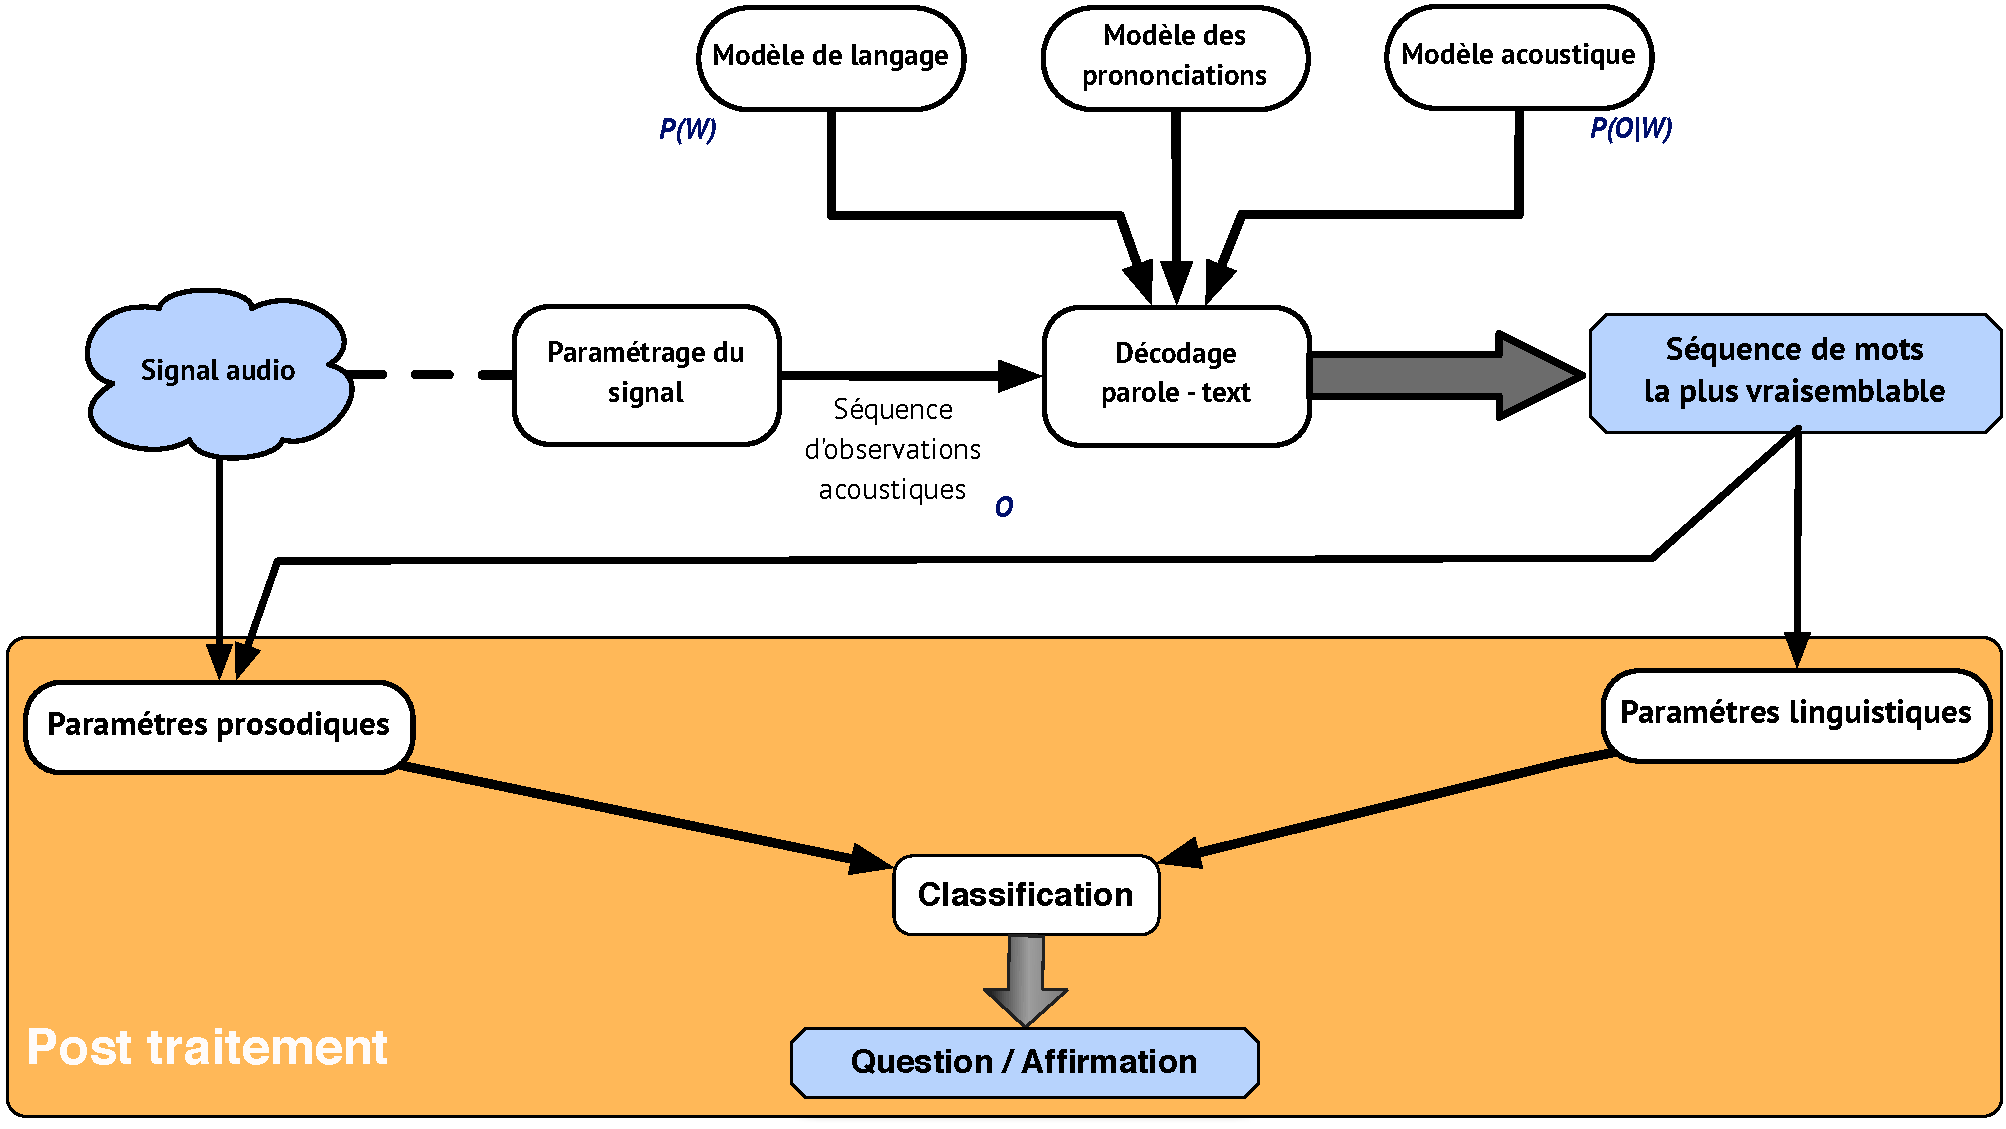
\includegraphics[scale=0.38]{images/pictures/QD_last.pdf}
\caption{Étape de post-traitement pour la détection de questions}
\label{Fig:QD}
\end{figure}

L'approche mise en place implique la définition de différents types de paramètres prosodiques et linguistiques permettant de faire la différence entre les questions et les affirmations.  

\minitoc


%=======================================================================
\section{Paramètres prosodiques}
\renewcommand{\rightmark}{Paramètres prosodiques}
%=======================================================================

Les classifieurs prosodiques ont l'objectif de détecter les phrases perçues comme des questions par le biais de l'intonation. 
Le choix des paramètres prosodiques résulte de l'avis général que les questions comportent une intonation finale montante.

La figure \ref{Fig:F0-quoi} présente la courbe de la fréquence fondamentale (F0) sur la phrase ``c'est quoi ?''.

\begin{figure}[h!]
\centering
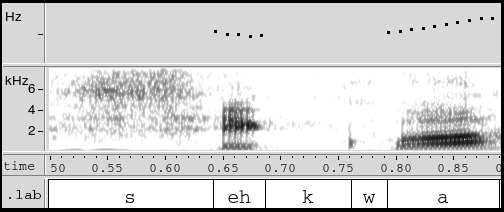
\includegraphics[scale=0.48]{images/pictures/quoi-F0-v2.png}
\caption{Courbe de la fréquence fondamentale (en haut) \\sur la phrase ``c'est quoi ?"}
\label{Fig:F0-quoi}
\end{figure}

Les caractéristiques prosodiques comprennent des informations liées à la durée, à l'énergie et à la fréquence fondamentale (F0). 
Deux ensembles de paramètres prosodiques sont considérés : un qui prend en compte la structure prosodique de la phrase et des informations a priori sur les locuteurs, et un autre qui est calculé sur différentes parties de la phrase. 

\hiddensubsection{Paramètres avec structure prosodique}

Un premier ensemble d'expériences considère seulement les données issues des transcriptions manuelles de référence, donc des transcriptions en mots parfaites, des informations a priori sur les différents locuteurs et des frontières temporelles parfaites sur les phrases.
Les frontières temporelles des mots et des phonèmes, obtenues par alignement forcé, sont supposées correctes. 
Dix paramètres prosodiques ont été utilisés afin de distinguer les questions des affirmations (voir Tab. \ref{Tab:prosodParams1}) : cinq sont associés à la dernière syllabe de la phrase (avec des normalisations par rapport à son groupe prosodique) et cinq autres sont calculés sur la partie finale de la phrase. 
Les groupes prosodiques de la phrase sont déterminés à partir des informations linguistiques (pour grouper des mots grammaticaux avec les mots lexicaux correspondants) et des informations prosodiques, comme décrit dans \cite{Bartkova:2013}. 

\begin{table}[h!]
\centering
\begin{tabular}{|r|l|}
\hline
id.	& description 										\\ \hline
P0	& la durée de la dernière voyelle (normalisée)						\\ % \hline
P1	& le logarithme de l'énergie de la dernière voyelle (normalisé)				\\ % \hline
P2	& la pente F0 sur la dernière voyelle 		 					\\ % \hline
P3	& la différence du F0 entre la dernière voyelle et la voyelle précédente 		\\ % \hline
P4	& P2 $\times$ P0$^2$									\\ % \hline
P5	& la pente de F0 calculée sur la plus longue pente finale de F0				\\ % \hline
P6	& la durée de la plus longue pente finale de F0 					\\ % \hline
P7	& la variation F0 entre le début et la fin de la plus longue pente finale de F0	 	\\ % \hline
P8	& P5 $\times$ P6$^2$									\\ % \hline
P9	& la valeur F0 en fin de phrase (normalisée par locuteur)				\\ \hline
\end{tabular}	
\caption{Les paramètres prosodiques qui prennent en compte la structure prosodique de la phrase et des informations a priori sur les locuteurs (pour la normalisation)}
\label{Tab:prosodParams1}
\end{table}

La durée de la dernière voyelle (\textit{P0}) est calculée à partir de la segmentation phonétique résultant de l'alignement forcé. 
Son énergie (\textit{P1}) correspond à la valeur moyenne calculée sur l'ensemble des trames de son segment. 
L'énergie et la durée de la voyelle sont ensuite normalisées par rapport aux valeurs moyennes calculées sur les autres voyelles du groupe prosodique courant. 
La pente F0 (\textit{P2}) est calculée par régression linéaire sur les trames de parole correspondant à la voyelle. 
La différence du F0 par rapport à la voyelle précédente (\textit{P3}) est aussi prise en compte. 
Le cinquième paramètre (\textit{P4}) est le produit entre la pente du F0 et la durée de la voyelle au carré (ce paramètre est inspiré du seuil de glissando).

D'autres paramètres, prosodiques, plus globaux, sont calculés sur la plus longue pente de F0 qui se termine dans la dernière syllabe de la phrase. 
A partir de la dernière syllabe, nous remontons dans le temps jusqu'à la détection d'une inversion de la pente de F0 (nommée ``pente finale"). 
Les paramètres calculés sur cette partie du signal sont : la pente de F0 (déterminée par régression linéaire) (\textit{P5}) , la durée de ce segment (\textit{P6}), la variation totale de F0 entre le début et la fin de la pente (\textit{P7}) , et également le produit entre la pente et le carré de la durée (\textit{P8}) . 
Un dernier paramètre prosodique (\textit{P9}) correspond au niveau de F0 à la fin de la phrase, exprimé en pourcentage de la plage de F0 du locuteur courant (0 correspondant à la valeur la plus base de F0 pour ce locuteur, 100 correspondant à la valeur la plus élevée de F0 pour ce locuteur).

\hiddensubsection{Paramètres sur segment arbitraire}

Des tests complémentaires ont été effectués en extrayant d'autres paramètres prosodiques sur la phrase entière, sur les dernières 700ms du signal ou sur les dernières 200ms du signal de la phrase. 
Ces tests n'utilisent aucune information a priori (sur les locuteurs ou autre) et n'effectuent donc pas des normalisations. 
Ils peuvent être appliqués sur des données transcrites manuellement (correctes) ou sur des données transcrites automatiquement (susceptibles de contenir des erreurs de mots). 


\begin{table}[h!]
\centering
\begin{tabular}{|r|l|}
\hline
id.	& description 									\\ \hline
C0	& la durée du segment (nombre de trames)					\\
C1	& la vitesse d'élocution (nombre de voyelles par seconde) 			\\ \hline
C2,C3	& la moyenne et l'écart type des logarithmes des énergies des voyelles  	\\ 
C4	& la pente des logarithmes des énergies  					\\
C5	& la pente ``finale" des logarithmes des énergies				\\ \hline
C6	& le nombre des trames ayant des valeurs F0 non-nulles	 			\\ 
C7,C8	& la moyenne et l'écart type des valeurs F0 (non-nulles) des voyelles 		\\
C9	& la valeur F0 en fin de phrase (non nulle) 					\\
C10	& la pente de F0 				 				\\ 
C11	& la pente ``finale" de F0 							\\ 
C12	& la pente de F0 minimale (sur segment isolé)					\\
C13	& la pente de F0 maximale (sur segment isolé)					\\ 
C14	& le nombre de pentes de F0 ascendantes (sur segments isolés)  			\\
C15	& le nombre de pentes de F0 descendantes (sur segments isolés)  		\\
C16	& la moyenne des pentes de F0 ascendantes (sur segments isolés) 		\\ 
C17	& la moyenne des pentes de F0 descendantes (sur segments isolés) 		\\ 
C18	& la déviation moyenne des pentes de F0 (sur segments isolés) 			\\ 
C19	& le nombre de pentes de F0 ascendantes (sur trames consécutives)	  	\\
C20	& le nombre de pentes de F0 descendantes (sur trames consécutives)  		\\
C21	& la moyenne des pentes de F0 ascendantes (sur trames consécutives) 		\\ 
C22	& la moyenne des pentes de F0 descendantes (sur trames consécutives) 		\\ 
C23	& la déviation moyenne des pentes de F0 (sur trames consécutives) 		\\ \hline
\end{tabular}
\caption{Les paramètres prosodiques calculés sur la phrase entière, sur les dernières 700ms du signal ou sur les dernières 200ms du signal}
\label{Tab:prosodParams2}
\end{table}

Vingt-quatre paramètres prosodiques ont été utilisés afin de distinguer les questions des affirmations : deux paramètres généraux (la durée du segment et la vitesse d'élocution), quatre paramètres liés à l'énergie et 18 paramètres liés à la fréquence fondamentale (voir Tab. \ref{Tab:prosodParams2}). 

Les frontières temporelles de voyelles sont extraites des alignements forcés à partir des transcriptions manuelles ou à partir des variantes de prononciation des mots issus des transcriptions automatiques. 

La durée de la phrase (C0) et la vitesse d'élocution (C1) servent comme indices pour identifier le type de parole, préparée ou spontanée. 
Dans la parole spontanée les phrases sont généralement plus courtes et prononcées plus rapidement. 

Toutes les pentes sont calculées par régression linéaire (sur les valeurs non-nulles). 

La pente ``finale" de F0 est calculée sur le dernier segment de la phrase qui ne présente pas d'inversion de la pente de F0 : à partir de la dernière trame, nous remontons dans le temps jusqu'à la détection d'une inversion de la pente de F0. 
La pente ``finale" des logarithmes des énergies et calculée sur le dernier segment de la phrase qui ne présente pas d'inversion de la pente des logarithmes des énergies. 

\begin{figure}[h!]
\centering
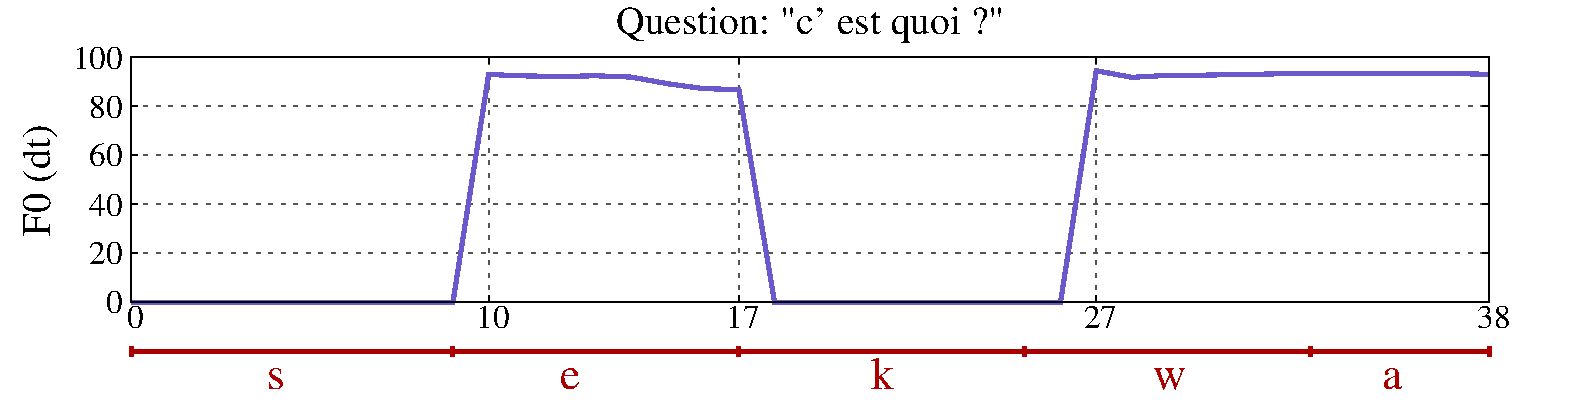
\includegraphics[scale=0.58]{images/results/F0prosody.pdf}
\caption{Exemple des segments ``isolés'' des fréquences fondamentales (F0)}
\label{Fig:exF0}
\end{figure}

Sept de nos paramètres prosodiques  (\{C12, C13, C14, C15, C16, C17, C18\}) sont calculés sur des segments ``isolés''. 
Un segment est considéré comme étant ``isolé'' s'il est entouré par des valeurs nulles. 
Dans l'exemple donné dans la figure \ref{Fig:exF0} (question ``c'est quoi?'' prononcée en 380ms), nous avons 2 segments isolés sur la fréquence fondamentale~: [10, 17], [27, 38]. 

Nous avons calculé la pente de la fréquence fondamentale sur chacun des segments ``isolés''. 
Une pente est considérée comme ascendante si elle a une valeur positive, et descendante - si elle a une valeur négative. 
Seuls les pentes non-nulles sont considérées dans le calcul des paramètres. 
La déviation moyenne des pentes de F0 sur segments isolés (C18) est calculée comme la valeur moyenne des pentes en valeur absolue. 

\begin{figure}[h!]
\centering
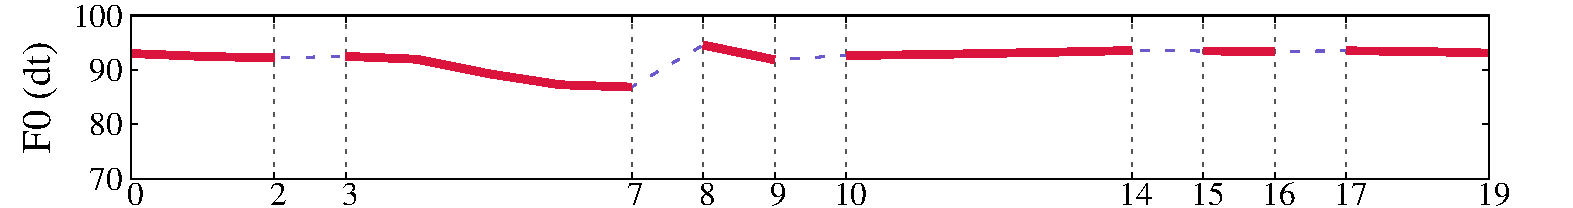
\includegraphics[scale=0.58]{images/results/F0prosody_c.pdf}
\caption{Exemple de segments de trames consécutives pour la fréquence fondamentale (F0)}
\label{Fig:exF0-c}
\end{figure}

Les cinq derniers paramètres (\{C19, C20, C21, C22, C23\}) sont calculés sur des trames consécutives en ignorant les valeurs nulles. 
Sur la séquence de valeurs F0 non-nulles, nous considérons les segments qui ont des valeurs F0 ascendantes ou descendantes et nous ignorons les transitions d'un segment à l'autre. 

Pour clarifier, l'exemple donné dans la figure \ref{Fig:exF0} contient 38 trames, dont 18 trames ont associée une valeur F0 nulle; la figure \ref{Fig:exF0-c} affiche la suite des valeurs F0 non-nulles sur 20 trames, après l'enlèvement des valeurs F0 nulles. 
Nous identifions ensuite sur la séquence de valeurs F0 non-nulles tous les changements de direction (ascendante ou descendante) de valeurs F0 : entre les trame [2, 3], [7, 8], [9, 10], [14, 15], [16, 17]. 
Les segments sur lesquels sont calculés les derniers cinq paramètres prosodiques sont : [0, 2], [3, 7], [8, 9], [10, 14], [15, 16], [17, 19] (les transitions d'un segment à l'autre sont ignorées).

%Nous identifions ensuite sur la séquence de valeurs F0 non-nulles tous les trames qui présentent un changement de direction (ascendante ou descendante) de valeurs F0 : entre les trame [3, 4], [5, 6], [7, 8], [13, 14], [15, 16], [21, 22], [23, 24]. 

%=======================================================================
\section{Paramètres linguistiques}
\renewcommand{\rightmark}{Paramètres linguistiques}
%=======================================================================

Les classifieurs linguistiques ont l'objectif de détecter les phrases perçues comme questions par le biais de formes interrogatives. 
Trois paramètres linguistiques sont considérés dans notre étude.

\hiddensubsection{Rapports de vraisemblance}

Deux de nos paramètres linguistiques (\textit{lexLLR - lexical log-likelihood ratio}, \linebreak \textit{synLLR - syntactic log-likelihood ratio}) sont représentés par le logarithme du rapport entre la vraisemblance d'une phrase par rapport au modèle de langage de questions et la vraisemblance de la phrase par rapport au modèle de langage d'affirmations \cite{Yuan:2005} :

\begin{equation}
LLR(phrase) = log \left ( \frac{P(phrase|ML-questions)}{P(phrase|ML-affirmations)}   \right )
\end{equation}

Une phrase qui a une valeur \textit{LLR} positive est susceptible d'être une question. 
Et vice-versa, une phrase ayant une valeur \textit{LLR}  négative est susceptible d'être une affirmation.

Pour calculer le rapport de vraisemblance lexical (\textit{lexLLR}) d'une phrase, nous appliquons les modèles de langage lexicaux (de questions et d'affirmations) sur sa séquence de mots.

Pour calculer le rapport de vraisemblance syntaxique (\textit{synLLR}) d'une phrase, nous appliquons les modèles de langage syntaxiques (de questions et d'affirmations) sur sa séquence de classes grammaticales (\acrshort{POS}).

\hiddensubsection{Présence de motifs interrogatifs}

Le troisième paramètre linguistique (\textit{iP - interrogative patterns}) indique la présence (1) ou l'absence (0) de motifs interrogatifs discriminatoires. 
Une phrase ayant un motif interrogatif est susceptible d'être une question. 

Une liste de motifs interrogatifs a été extraite à partir des questions appartenant au corpus GigaWord avec une version modifiée de l'outil PrefixSpan \cite{Pei:2001} qui ne considère que des séquences consécutives de mots. 
Leur fréquences d'occurrence ont été ensuite comparées entre les transcriptions de questions et d'affirmations~: les séquences ayant des fréquences similaires ont été ignorées. 
Les séquences sans aucun sens interrogatif ont été supprimées à la main (40 séquences). 

La liste finale de motifs interrogatifs est : \{quel, quelle, quels, quelles, comment, combien, pourquoi, est ce que, est ce qu', qu' est ce, qu' est ce que, qu' est ce qu'\}.





%=======================================================================
\chapter{Expérimentations}
\renewcommand{\leftmark}{Expérimentations}
%=======================================================================

Trois types différents de paramètres sont étudiés : le classifieur basé uniquement sur des paramètres prosodiques, le  classifieur basé uniquement sur des paramètres linguistiques et le classifieur combiné, basé sur des paramètres prosodiques et linguistiques. 
Différentes combinaisons de paramètres sont également analysées. % dans le but d'évaluer leur utilité. 

L'évaluation de classifieurs est faite sur des transcriptions manuelles et sur des sorties d'un système de reconnaissance vocale.

Les tests effectués sur des informations issues des transcriptions manuelles ont pour but d'évaluer la performance maximale pouvant être obtenue dans des conditions idéales (transcription parfaite, segmentation parfaite). Les paramètres linguistiques sont extraits à partir des transcriptions manuelles de signaux audio et les paramètres prosodiques - à partir de la segmentation phonétique résultant de l'alignement forcé. 
Des informations a priori sur les locuteurs sont extraites des annotations manuelles des signaux audio (disponibles dans les fichiers .STM), qui permettent de normaliser si besoin les valeurs de la fréquence fondamentale (F0) pour chaque locuteur. 

Les tests effectués sur des informations issues des transcriptions automatiques, obtenues avec un système de reconnaissance grand vocabulaire, ont pour but d'évaluer la performance dans des conditions réelles. La détection de questions sur les transcriptions automatiques d'un système de reconnaissance vocale pose plusieurs problèmes : les transcriptions sont susceptibles de contenir des erreurs de reconnaissance sur les mots et les frontières de phrases sont susceptibles d'être mal placées. 
Si les frontières temporelles de phrases sont mal placées, certains mots peuvent manquer ou être en trop et les paramètres prosodiques seront calculés sur le mauvais segment.  
Dans la première série d'expériences (sections \ref{sec:prosod}, \ref{sec:ling}, \ref{sec:comb} et \ref{sec:comp}) nous considérons les frontières de phrases parfaites, telles que définies dans les transcriptions manuelles.

\minitoc

\newpage

%=======================================================================
\section{Utilisation des paramètres prosodiques}
\label{sec:prosod}
\renewcommand{\rightmark}{Utilisation des paramètres prosodiques}
%=======================================================================

Les études sur les paramètres prosodiques analysent l'impact de la zone d'extraction et du jeu de paramètres. 
Le calcul des paramètres prosodiques utilise des informations liées aux frontières temporelles de la phrase et des voyelles, ce qui explique des analyses séparées sur des transcriptions manuelles et sur des transcriptions automatiques, et leur différence de performance. 

\begin{figure}[h!]
\begin{subfigure}{\textwidth}
\centering
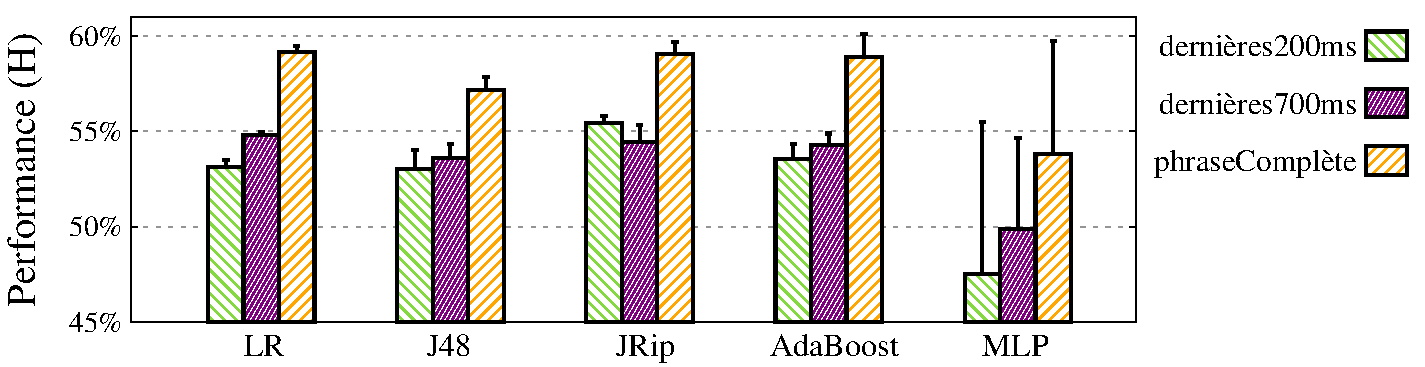
\includegraphics[scale=0.56]{images/results/prosodicZones_onDecodings.pdf} 
\caption{transcriptions automatiques}
\end{subfigure}
\begin{subfigure}{\textwidth}
\centering
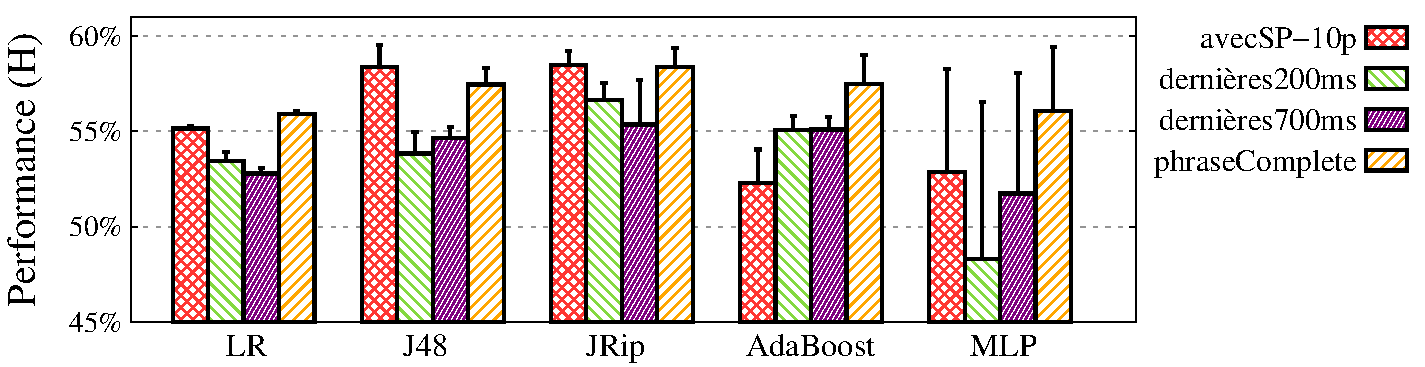
\includegraphics[scale=0.56]{images/results/prosodicZones_onTranscripts.pdf}
\caption{transcriptions manuelles}
\end{subfigure}
\caption{Résultats (moyenne harmonique) obtenus en fonction des différentes zones d'extraction de paramètres prosodiques, lors de l'utilisation des transcriptions automatiques (a) ou des transcriptions manuelles (b)}
\label{Fig:QD-p-pZones}
\end{figure}


Les résultats obtenus en fonction des différentes zones d'extraction de paramètres prosodiques sont présentés dans la figure \ref{Fig:QD-p-pZones}. 
Dans nos expériences, un groupe de 10 paramètres prosodiques tient compte de la structure prosodique de la phrase et de l'identité des locuteurs ('avecSP-10p') et un autre groupe de 24 paramètres prosodiques est extrait sur la phrase entière ('phraseComplète'), des dernières 700ms de la phrase ('dernières700ms') et des dernières 200ms de la phrase ('dernières200ms'). 
Les paramètres avec la structure prosodique ('avecSP-10p') sont calculés uniquement sur les transcriptions manuelles. 

Les paramètres extraits sur les dernières 700ms de la phrase offrent de meilleures performances que les paramètres extraits sur les dernières 200ms de la phrase, avec les classifieurs J48, AdaBoost et MLP, quelque soit le type de transcriptions (manuelles ou automatiques). 
La performance du classifieur à base de réseaux de neurones (MLP) varie beaucoup en fonction des différents ensembles d'apprentissages, peu importe le type de paramètres prosodiques ou le type de données. 
Les paramètres qui prennent en compte des informations a priori sur les locuteurs et de la structure prosodique de la phrase ('avecSP-10p') donnent des résultats variables selon les différents classifieurs. 
La meilleure performance sur les transcriptions automatiques est acquise avec les paramètres prosodiques calculés sur la phrase complète. 
Dans les expérimentations suivantes, seuls les paramètres extraits sur la phrase complète seront considérés. 

\begin{figure}[h!]
\centering
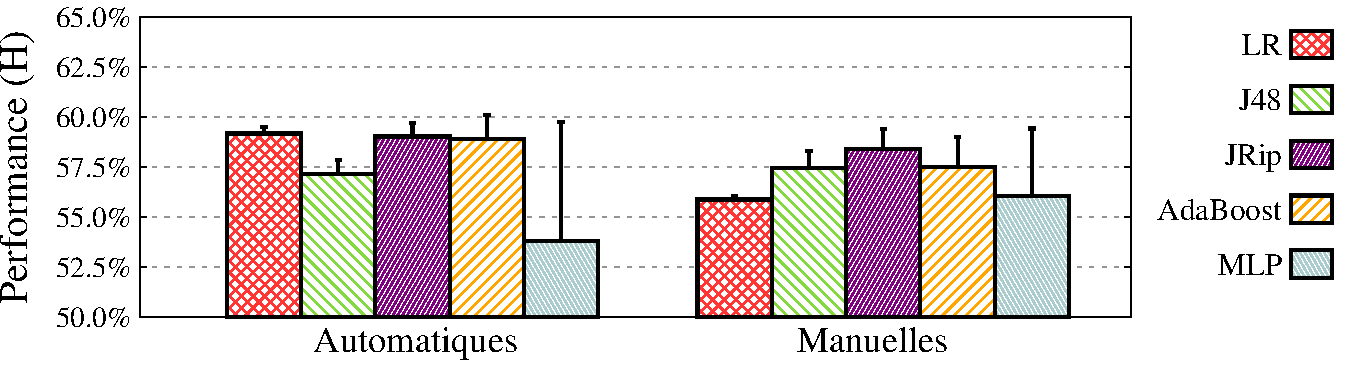
\includegraphics[scale=0.56]{images/results/prosodicClassifier_completeSentence_compareManualVsAutomatic.pdf}
\caption{Performance (moyenne harmonique) obtenue avec les différents types de classifieurs en utilisant les paramètres prosodiques `phraseComplète' sur les transcriptions automatiques et  sur les transcriptions manuelles}
\label{Fig:QD-P-MvsA}
\end{figure}

Les performances moyennes  des différents classifieurs sont affichées dans la figure \ref{Fig:QD-P-MvsA}. 
La meilleure performance obtenue avec les paramètres prosodiques sur les transcriptions automatiques est de 59,19\% (classifieur LR) et sur les transcriptions manuelles - 58,40\% (classifieur JRip). 

\begin{figure}[h!]
\centering
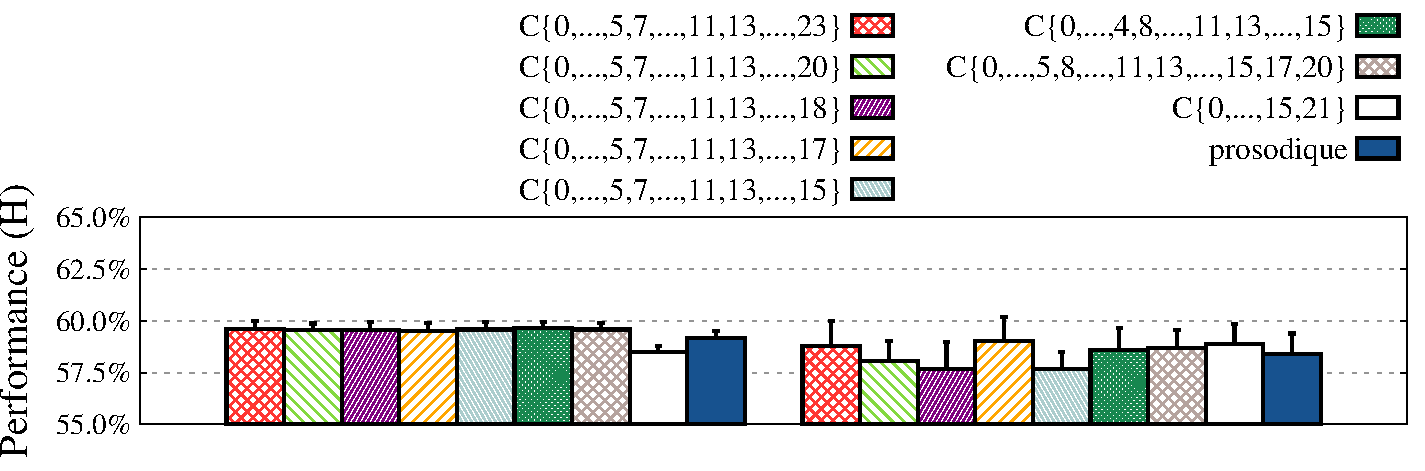
\includegraphics[scale=0.59]{images/results/completeSentence_compareProsodicFeatures.pdf}
\caption{Impact du choix des paramètres prosodiques calculés sur la phrase complète, lors de l'utilisation du classifieur LR sur les transcriptions automatiques et du classifieur JRip sur les transcriptions manuelles}
\label{Fig:QD-p-PFeatures-JRip-LR}
\end{figure}

Diverses combinaisons des paramètres prosodiques (choisis ad-hoc ou avec l'algorithme de sélection `AttributeSelectedClassifier' de WEKA) ont été évaluées dans le but de déterminer le meilleure choix de paramètres. Un sous-ensemble des résultats obtenus avec le classifieur LR sur transcriptions automatiques et avec le classifieur JRip sur transcriptions manuelles est présenté dans la figure \ref{Fig:QD-p-PFeatures-JRip-LR}. 
Les comportements sont différents entre les transcriptions automatiques et les transcriptions manuelles : les performances obtenues sur les transcriptions automatiques avec les divers choix de paramètres sont similaires et supérieures à l'utilisation des 24 paramètres (seule exception, la combinaison C\{0,...,15,21\}), alors que les les performances obtenues sur les transcriptions manuelles varient beaucoup d'une combinaison à l'autre.  
Sur les transcriptions automatiques, les deux meilleures combinaisons de paramètres sont C\{0,...,5,7,...,11,13,...,23\} (H=59,61\%) et C\{0,...,4,8,...,11,13,...,15\} (H=59,65\%). 
Sur les transcriptions manuelles, les deux meilleures combinaisons de paramètres sont C\{0,...,5,7,...,11,13, ...,17\} \linebreak (H=59,02\%) et C\{0,...,15,C21\} (H=58,87\%). 
Pour faire un compromis entre les gains obtenus sur transcriptions automatiques et les gains obtenus sur transcriptions manuelles, nous avons choisi d'utiliser la première combinaison de paramètres, C\{0,...,5,7, ...,11,13, ...,23\}, qui conserve 22 paramètres (en ignorant les paramètres C6 - le nombre des trames ayant des valeurs F0 non-nulles, et C12 - la pente de F0 minimale sur segment isolé). 

Une analyse plus détaillée des résultats obtenus avec le classifieur à base d'une régression logistique (LR) sur les transcriptions automatiques, en utilisant les 22 paramètres prosodiques appris sur le sixième ensemble d'apprentissage (sur lequel le classifieur atteignait la performance maximale) montre que 658 questions sur 940 et 4056 affirmations sur 7708 étaient correctement classées, ce qui correspond à des pourcentages de questions correctement classées de 70,00\% et d'affirmations correctement classées de 52,62\% (cf. Tab. \ref{Tab:p-LR-1trial-MC}). 
La moyenne harmonique correspondante est de H=60,08\%. 

\begin{table}[h!]
\centering
\begin{tabular}{|r|r|r|r|r}
\cline{2-4}
\multicolumn{1}{c|}{} 	& \multirow{2}{*}{nombre}	& classé comme 	& classé comme 	& 				\\ 
\multicolumn{1}{c|}{} 	& 				& question 	& affirmation 	& 				\\ \cline{1-4} 
question		&   940				& \textbf{658}	& 282		& questionsCC=70,00\%		\\ \cline{1-4} 
affirmation		&  7708				&  3652		& \textbf{4056}	& affirmationsCC=52,62\%	\\ \cline{1-4}	
\end{tabular}
\caption{Matrice de confusion question/affirmation obtenue avec le classifieur LR sur 22 paramètres prosodiques ('phraseComplète') extraits des transcriptions automatiques}
\label{Tab:p-LR-1trial-MC}
\end{table}


%=======================================================================
\section{Utilisation des paramètres linguistiques}
\label{sec:ling}
\renewcommand{\rightmark}{Utilisation des paramètres linguistiques}
%=======================================================================

Les performances obtenues avec nos 3 paramètres linguistiques sur les  transcriptions automatiques et manuelles sont affichées dans la figure \ref{Fig:QD-L-MvsA}. 

\begin{figure}[h!]
\centering
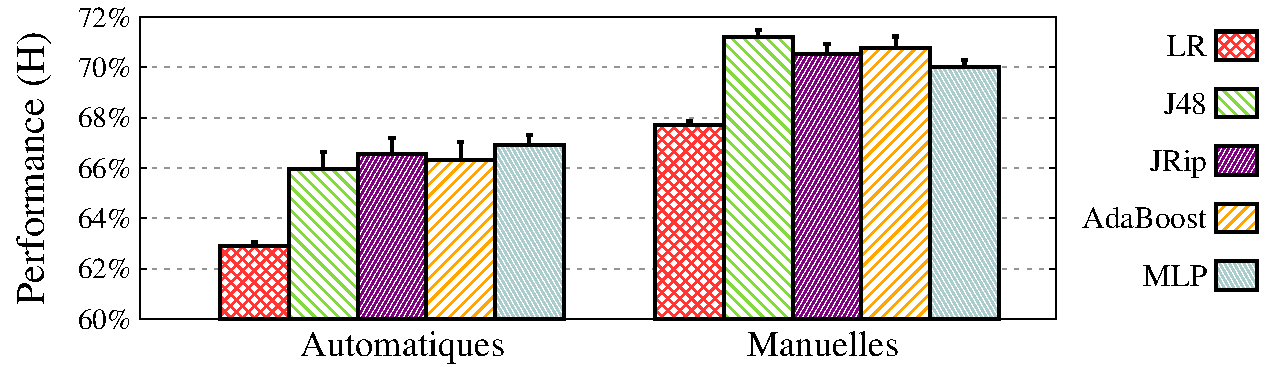
\includegraphics[scale=0.56]{images/results/linguisticClassifier_compareManualVsAutomatic.pdf}
\caption{Performance (moyenne harmonique) obtenue avec les différents classifieurs utilisant des paramètres linguistiques sur les transcriptions automatiques et sur les transcriptions manuelles}
\label{Fig:QD-L-MvsA}
\end{figure}

La différence de performance entre les transcriptions automatiques et les transcriptions manuelles est d'environ 5\% en valeur absolue, en raison d'erreurs de reconnaissance (taux d'erreur mot de 22\% sur ESTER2 et de 28\% sur ETAPE) et probablement à la mauvaise reconnaissance de mots interrogatifs. 
Les meilleures performances moyennes sont obtenues avec le  classifieur MLP sur les transcriptions automatiques (H=66,92\%) et avec le classifieur J48 sur les transcriptions manuelles (H=71,21\%). 

Les performances moyennes obtenues avec le classifieur MLP sur les transcriptions automatiques et avec le classifieur J48 sur les transcriptions manuelles, en utilisant différentes combinaisons de paramètres linguistiques, montrent l'importance de conserver les trois paramètres (cf. Fig. \ref{Fig:QD-L-LFeatures-MLP-J48}). 
Le paramètre linguistique le plus important est le rapport de vraisemblance lexical (lexLLR), avec les motifs interrogatifs (iP) et le rapport de vraisemblance syntaxique (synLLR) fournissant des informations complémentaires. 

\begin{figure}[h!]
\centering
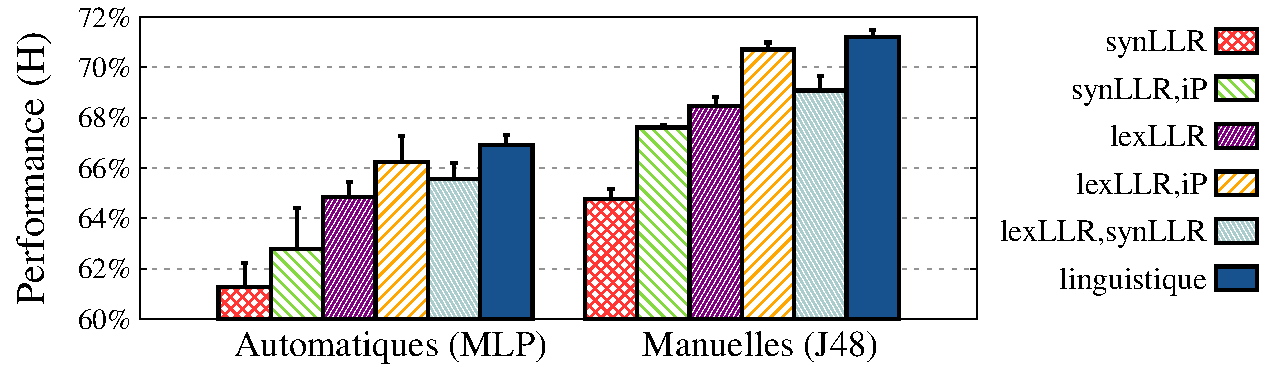
\includegraphics[scale=0.56]{images/results/compareLinguisticFeatures.pdf}
\caption{Impact du choix des paramètres linguistiques lors de l'utilisation du classifieur MLP sur les transcriptions automatiques et du classifieur J48 sur les transcriptions manuelles}
\label{Fig:QD-L-LFeatures-MLP-J48}
\end{figure}

Une analyse plus détaillée sur les résultats obtenus avec le classifieur MLP sur les transcriptions automatiques  en utilisant des paramètres linguistiques appris sur le neuvième ensemble d'apprentissage (sur lequel le classifieur atteignait la performance maximale) montre que 671 questions sur 940 et 4921 affirmations sur 7708 étaient correctement classées, ce qui correspond à des pourcentages d'identification correcte de questions de 71,38\% et d'affirmations de 63,84\% (cf. Tab. \ref{Tab:l-MLP-1trial-MC}). 
La moyenne harmonique est de H=67,40\%. 


\begin{table}[h!]
\centering
\begin{tabular}{|r|r|r|r|r}
\cline{2-4}
\multicolumn{1}{c|}{} 	& \multirow{2}{*}{nombre}	& classé comme 	& classé comme 	& 				\\ 
\multicolumn{1}{c|}{} 	& 				& question 	& affirmation 	& 				\\ \cline{1-4} 
question		&   940				& \textbf{671}	& 269		& questionsCC=71,38\%		\\ \cline{1-4} 
affirmation		&  7708				&  2787		& \textbf{4921}	& affirmationsCC=63,84\%	\\ \cline{1-4}	
\end{tabular}
\caption{Matrice de confusion question/affirmation obtenue avec le classifieur MLP  sur les paramètres linguistiques extraits des transcriptions automatiques}
\label{Tab:l-MLP-1trial-MC}
\end{table}



%=======================================================================
\section{Utilisation des paramètres combinés}
\label{sec:comb}
\renewcommand{\rightmark}{Utilisation des paramètres combinés}
%=======================================================================

Ces expériences sont basées sur un nouveau vecteur de paramètres regroupant les paramètres linguistiques et les paramètres prosodiques. 
Chaque phrase du corpus est donc représentée par un vecteur de 27 paramètres. 

Les performances obtenues avec les 27 paramètres combinés sur les  transcriptions automatiques et manuelles sont présentées dans la figure \ref{Fig:QD-C-MvsA}. 
La différence de performance entre les transcriptions automatiques et les transcriptions manuelles est d'environ 5\% en valeur absolue. 
Les meilleures performances moyennes sont obtenues avec le classifieur JRip sur les transcriptions automatiques (H=68,07\%) et avec le  classifieur LR sur les transcriptions manuelles (H=72,34\%). 

\begin{figure}[h!]
\centering
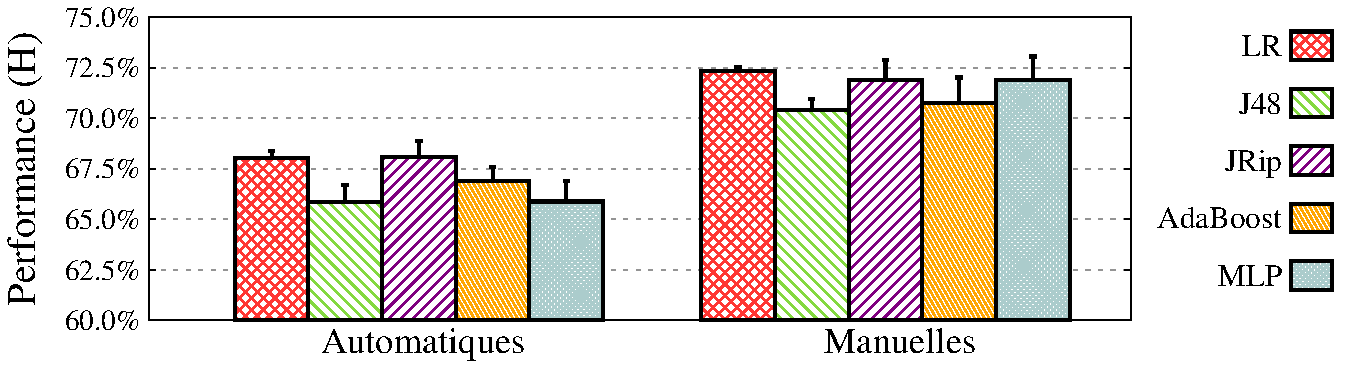
\includegraphics[scale=0.55]{images/results/combinedClassifier_compareManualVsAutomatic.pdf}
\caption{Performance (moyenne harmonique) obtenue avec les différents classifieurs combinés sur les transcriptions automatiques et manuelles}
\label{Fig:QD-C-MvsA}
\end{figure}

Diverses combinaisons des paramètres prosodiques et linguistiques (choisis ad-hoc ou avec l'algorithme de sélection `AttributeSelectedClassifier' de WEKA) ont été évaluées dans le but de déterminer le meilleure choix de paramètres. 
Un sous-ensemble des résultats obtenus avec le classifieur JRip sur transcriptions automatiques et avec le classifieur LR sur transcriptions manuelles est présenté dans la figure \ref{Fig:QD-C-CFeatures-JRip}. 
Dans les combinaisons évaluées, il apparaît qu'il est plus utile de conserver l'ensemble des 3 paramètres linguistiques (3L), plutôt qu'une sous-partie de ceux-ci.  

\begin{figure}[h!]
\centering
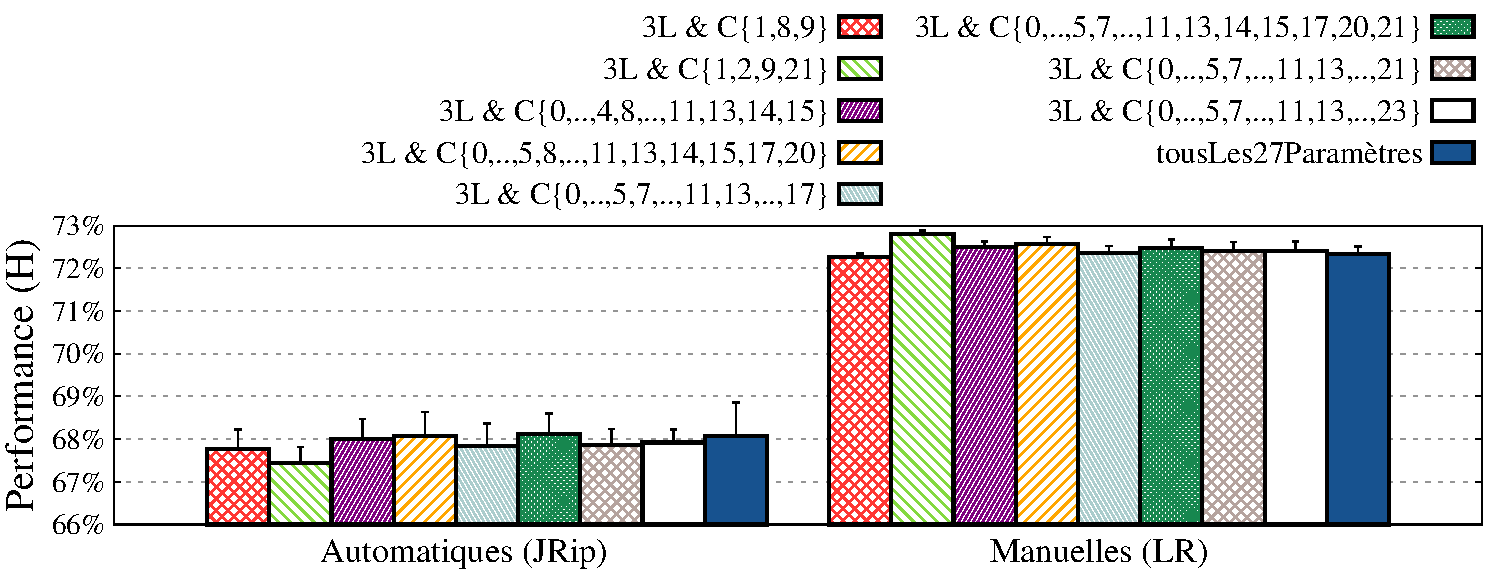
\includegraphics[scale=0.54]{images/results/combinedClassifier_compareFeatures.pdf}
\caption{Impact du choix des paramètres (prosodiques et linguistiques) lors de l'utilisation du classifieur JRip sur les transcriptions automatiques et du classifieur LR sur les transcriptions manuelles}
\label{Fig:QD-C-CFeatures-JRip}
\end{figure}

La meilleure performance obtenue sur les transcriptions automatiques correspond à l'utilisation des 27 paramètres prosodiques-linguistiques. 
La combinaison `3L \& C\{0,..,5, 7,..,11,13,14,15,17,20,21\}' offre seulement une très légère amélioration en comparaison. 
Les différentes combinaisons de paramètres offrent des performances entre 72,26\% et 72,81\% sur les transcriptions manuelles, à comparer à la performance de 72,34\% obtenue avec tous les paramètres. 
La meilleure performance est obtenue avec la deuxième combinaison de paramètres (3L \& C\{1,2,9,21\}), mais cette combinaison dégrade la performance sur transcriptions automatiques. 
En revanche, la quatrième combinaison (3L \& C\{0,..,5,8,..,11,13,14,15,17,20\}) offre une amélioration de 0,22 sur les transcriptions manuelles et pas de dégradation sur les  transcriptions automatiques. 
Compte tenu des faibles améliorations obtenues avec les différentes combinaisons de paramétrés, la totalité de paramètres sera conservée dans la suite des expériences. 

Les résultats obtenus avec le classifieur JRip sur les transcriptions automatiques  en utilisant des paramètres combinés appris sur le huitième ensemble d'apprentissage (sur lequel le classifieur atteignait la performance maximale) montre que 631 questions sur 940 et 5572 affirmations sur 7708 étaient correctement classées, ce qui corresponde à des pourcentages de classification correcte de questions de 67,13\% et d'affirmations de 72,29\% (cf. Tab. \ref{Tab:C-JRip-automatic}). 
La moyenne harmonique est de H=69,61\%.

\begin{table}[h!]
\centering
\begin{tabular}{|r|r|r|r|r}
\cline{2-4}
\multicolumn{1}{c|}{} 	& \multirow{2}{*}{nombre}	& classé comme 		& classé comme 	& 				\\ 
\multicolumn{1}{c|}{} 	& 				& question 		& affirmation 	& 				\\ \cline{1-4} 
question		&   940				& \textbf{631}  	& 309		& questionsCC=67,13\%		\\ \cline{1-4} 
affirmation		&  7708				& 2136			& \textbf{5572} & affirmationsCC=72,39\%	\\ \cline{1-4}	
\end{tabular}
\caption{Matrice de confusion question/affirmation obtenue avec le classifieur JRip  sur les paramètres combinés extraits des transcriptions automatiques}
\label{Tab:C-JRip-automatic}
\end{table}

La performance de ce système en termes de F-mesure (entre le rappel et la précision) est présentée dans le tableau \ref{Tab:Fmeasure-max} en annexe. 
Le tableau \ref{Tab:Fmeasure-Random} en annexe indique la performance d'un système qui répond au hasard.

%=======================================================================
\section{Comparaisons entre paramètres}
\label{sec:comp}
\renewcommand{\rightmark}{Comparaisons entre paramètres}
%=======================================================================

Cette section a comme objectif de comparer les résultats obtenus avec les classifieurs utilisant des paramètres prosodiques (24 paramètres), linguistiques (3 paramètres) et combinés (27 paramètres). 

\begin{figure}[h!]
\begin{subfigure}{\textwidth}
\centering
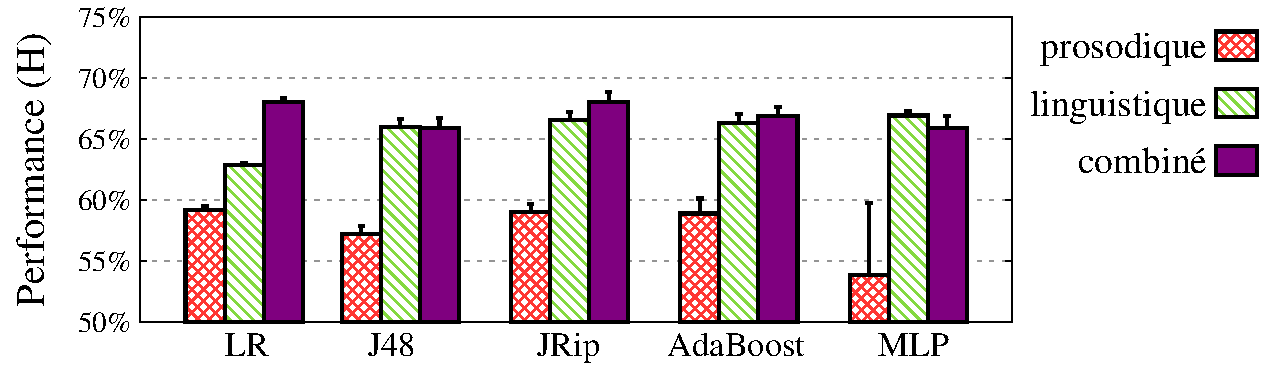
\includegraphics[scale=0.58]{images/results/comparePLC_onAutomatic_legendPLC.pdf}
\caption{transcriptions automatiques}
\end{subfigure}
\begin{subfigure}{\textwidth}
\centering
\includegraphics[scale=0.58]{images/results/comparePLC_onManual_legendPLC.pdf}
\caption{transcriptions manuelles}
\end{subfigure}
\caption{Performance (moyenne harmonique) obtenue sur les transcriptions automatiques (a) et sur les transcriptions manuelles (b), lors de l'utilisation des paramètres prosodiques, linguistiques et combinés}
\label{Fig:QD-PLC-MD}
\end{figure}

La figure \ref{Fig:QD-PLC-MD} présente les résultats obtenus avec les cinq algorithmes de classification lors de l'utilisation de paramètres prosodiques, linguistiques et combinés sur les transcriptions manuelles et sur les transcriptions automatiques. 
Les classifieurs prosodiques sont surpassés par les classifieurs linguistiques, qui sont surpassés par les classifieurs combinés (seules exceptions le classifieur J48 - peu importe le type de données, et le classifieur MLP - sur les transcriptions automatiques). 
Les écarts de performance obtenues avec les 3 types différents de paramètres varient en fonction du classifieur et des données traitées (manuelles ou automatiques). 


\begin{table}[h!]
\centering
\begin{tabular}{|l|r|r|}
\hline
\textbf{Données d'évaluation} 	& \textbf{\#questions} & \textbf{\#affirmations} \\ \hline
ESTER2		 	& 176	& 2163		\\ 
ETAPE		 	& 764	& 5545		\\ \hline
ESTER2 \& ETAPE	 	& 940	& 7708		\\ \hline
\end{tabular}
\caption{Description des données d'évaluation par sous corpus}
\label{Tab:TestData-QD-perCorpus}
\end{table}


Pour rappel, les différents classifieurs sont évalués sur les ensembles d'évaluation et de test de corpus ESTER2 et ETAPE, qui contiennent un total de 940 questions et 7708 affirmations. Dans la suite de cette section nous allons détailler les performances obtenues séparément sur le corpus ESTER2 et sur le corpus ETAPE.

\begin{figure}[h!]\begin{subfigure}{\textwidth}
\centering
\includegraphics[scale=0.6]{images/results/ETAPE_comparePLC_onAutomatic.pdf}
\caption{ETAPE}
\end{subfigure}
\begin{subfigure}{\textwidth}
\centering
\includegraphics[scale=0.6]{images/results/ESTER_comparePLC_onAutomatic.pdf}
\caption{ESTER2}
\end{subfigure}
\caption{Performance (moyenne harmonique) obtenue avec les différents classifieurs sur les transcriptions automatiques du corpus ETAPE (a) et du corpus ESTER2 (b)}
\label{Fig:QD-ESTER-ETAPE}
\end{figure}


Les performances de classification obtenues sur les transcriptions automatiques d'ESTER2 (discours préparé) et d'ETAPE (parole spontanée) sont presentées dans la figure \ref{Fig:QD-ESTER-ETAPE}. 
Les données appartenant à ESTER2 (performance moyenne de 72\% avec le classifieur JRip) sont plus faciles à classer que les données appartenant à ETAPE (performance moyenne de 66\% avec le classifieur LR). 


Les performances moyennes (moyenne harmonique, taux de questions correctement classées, taux d'affirmations correctement classées) obtenues sur les données appartenant au corpus ETAPE et au corpus ESTER2, lors de l'utilisation des paramètres prosodiques, linguistiques ou combinés sont présentées dans la figure \ref{Fig:ccq-ccS-Ester-Etape} (plus de détails dans les tableaux \ref{Tab:ccq-ccS-Ester-Etape-a}, \ref{Tab:ccq-ccS-Ester-Etape-m} en annexe). 

\begin{figure}[h!]
\centering
\includegraphics[scale=0.59]{images/results/compareData_PLC_HQS_EE.pdf}
\caption{Performances moyennes (moyenne harmonique H, taux de questions correctement classées qCC, taux d'affirmations correctement classées aCC) obtenues avec la combinaison de 5 algorithmes de classification par vote majoritaire sur les transcriptions automatiques et sur les transcriptions manuelles appartenant au corpus ETAPE (a) et au corpus ESTER2 (b)}
\label{Fig:ccq-ccS-Ester-Etape}
\end{figure}


Les évaluations sont effectuées avec la combinaison des 5 algorithmes de classification par vote majoritaire (qui définit le comportement global des 5 algorithmes).  
Sur le corpus ETAPE, les paramètres prosodiques ont une meilleure performance sur les questions, le taux d'affirmations correctement classés étant inférieur à 50\%. 
Sur le corpus ESTER2, les paramètres linguistiques et combinés ont une meilleure performance sur les affirmations, le taux de questions correctement classés étant généralement inférieur à 60\% (seule exception avec les paramètres combinés sur transcriptions manuelles). 

Les paramètres combinés donnent des meilleures performances que les paramètres prosodiques ou les paramètres linguistiques, quelque soit le corpus de parole (ESTER2 ou ETAPE) ou le type de données (manuelles ou automatiques). 
De plus, l'utilisation des paramètres combinés réduit l'écart de performance entre les résultats obtenus sur questions et les résultats obtenus sur affirmations.  

%=======================================================================
\section{Impact des frontières sur la performance}
\renewcommand{\rightmark}{Impact des frontières sur la performance}
%=======================================================================

Pour évaluer la perte de performance lorsque les frontières des phrases ne sont pas parfaites, nous avons modifié les frontières prédéfinies des phrases pour simuler des erreurs introduites par une segmentation automatique,  de trois façons différentes : 

\begin{itemize}
\item en décalant chaque frontière (gauche ou droite) avec une valeur choisie aléatoirement de \{-300, -200, -100, +100, +200 ou +300\}ms. Si le nouveau segment contient que des silences/bruits ou il est absent dans la transcription automatique, la phrase est ignorée dans cette évaluation  (6\% de questions et 4\% d'affirmations)
\item en décalant chaque frontière (gauche ou droite) avec une valeur choisie aléatoirement de \{-1000, -800, -600, -400, -200, +200, +400, +600, +800 ou +1000\}ms. Si le nouveau segment contient que des silences/bruits ou il est absent dans la transcription automatique, la phrase est ignorée dans cette évaluation (8\% de questions et 4\% d'affirmations)
\item en extrayant le plus long segment délimité par des silences : le segment de référence est étendu avec les 5 unités précédentes (mots, silences et/ou bruits) et les 5 unités suivantes (mots, silences et/ou bruits); on cherche ensuite dans ce segment étendu le premier et le dernier segment de silence qui vont définir les nouvelles frontières de la phrase : la frontière gauche est le temps de fin du premier segment de silence et la frontière droite est le temps de début du dernier segment de silence. En fonction de la position de ces segments de silence, la phrase de référence va être étendue (silences à l'extérieur de la phrase) ou rétrécie (silences à l'intérieur de la phrase). Si les segments de silence recherchés sont absents dans le segment étendu, la phrase est ignorée dans cette évaluation (0.5\% de questions et 0.3\% d'affirmations)     
\end{itemize}

La perte de performance de classification lors de la modification des frontières prédéfinies des phrases sur les transcriptions automatiques est évalué dans la figure \ref{Fig:QD-automatic-differentBorders}. 

\begin{figure}[h!]
\centering
\includegraphics[scale=0.58]{images/results/differentBoundaries-JRip_onAutomatic_legendPLC.pdf}
\caption{Performance (moyenne harmonique) obtenue avec le classificateur JRip sur les transcriptions automatiques lors de la modification des frontières prédéfinies}
\label{Fig:QD-automatic-differentBorders}
\end{figure}

Le classifieur prosodique est le plus dépendant de la position des frontières, sa perte de performance atteint jusqu'à 23,82\% sur les segments délimités par des silences. 
Avec le classifieur linguistique, la perte de performance varie entre 2,15\% (aléatoire $\pm$300ms) et 3,93\% (frontières de silences). 
Le classifieur linguistique dépasse même la performance du classifieur combiné sur les segments délimités par des silences. 
Avec le classifieur combiné, la perte de performance varie entre 2,54\% (en modifiant les frontières prédéfinies avec une valeur aléatoire de $\pm$300ms) et 7,79\% (en remplaçant la phrase avec un segment délimité par des silences). 
Ces résultats montrent l'importance de bien définir les frontières de phrases pour la tâche de la détection de questions. 
Cependant, pour des petites variations dans les frontières prédéfinies ($\pm$300ms, $\pm$1000ms), notre classifieur parvient toujours à classer correctement 65\% d'entrées questions / affirmations.  


Une dernière expérience a consisté à combiner les sorties des cinq algorithmes de classification, en utilisant les 27 paramètres prosodiques-linguistiques. 
Les performances moyennes (H) obtenues avec les cinq classifieurs séparément, et avec leur combinaison (par vote majoritaire) sont présentés dans le tableau \ref{Tab:votemajoritaire}. 
La performance du vote majoritaire dépasse légèrement celle des 5 classifieurs sur les transcriptions manuelles  et sur les transcriptions automatiques avec des frontières prédéfinies ou modifiées de manière aléatoire (avec un gain de performance entre 0,36\% et 0.92\%). 
Les classifieurs J48, JRip et AdaBoost ont une meilleure performance comparée à celle du vote majoritaire sur les transcriptions automatiques délimitées par des silences.  

\begin{table}[h!]
\centering
\begin{tabular}{|r|r|r|r|r|r|} 
\hline
\multirow{3}{*}{Classifieur} 	& \multirow{3}{*}{manuelles} & \multicolumn{4}{c|}{automatiques}	\\ \cline{3-6}
				&				& frontières 	& aléatoire  		& aléatoire	& frontières	\\
				&				& prédéfinies 	& +/-300ms		& +/-1000ms	& silence	\\ \hline
LR				& 72,34				& 68,04		& 64,91			& 62,81		& 50,07		\\ 
J48				& 70,42				& 65,87 	& 63,78			& 62,35		& 60,77		\\ 
JRip				& 71,91				& 68,07		& 65,53			& 64,03		& 60,28		\\ 
AdaBoost			& 70,75				& 66,91		& 63,84			& 62,73		& 63,17		\\ 
MLP				& 71,88				& 65,88		& 63,16			& 61,91		& 56,81		\\ \hline 
vote majoritaire		& 73,26				& 68,69		& 65,89			& 64,89		& 58,96		\\ \hline
\end{tabular}
\caption{Performance (moyenne harmonique) obtenue avec les 5 classifieurs et avec leur combinaison (par vote majoritaire) sur les transcriptions manuelles et automatiques} 
\label{Tab:votemajoritaire}
\end{table}



%%%%%%%%%%%%%%%%%%%%%%%%%%%%%%%%%%%%%%%%%%%%%%%%%%%%%%%%%%%%%%%%%%%%%%%%%%%%
\chapter{Conclusions}
\renewcommand{\leftmark}{Conclusions}
\renewcommand{\rightmark}{Conclusions}
%%%%%%%%%%%%%%%%%%%%%%%%%%%%%%%%%%%%%%%%%%%%%%%%%%%%%%%%%%%%%%%%%%%%%%%%%%%%

Cette partie a analysé la détection de la modalité des phrases (questions versus affirmations) en français à partir de transcriptions manuelles ou automatiques. 
Les personnes sourdes ou malentendantes ont besoin d'une détection automatique de questions afin d'être informées qu'une question leur a été posée et qu'ils doivent répondre ou demander des clarifications. 

Pour répondre à ce défi, des paramètres prosodiques ont été extraits à partir du signal audio (en utilisant des informations sur les frontières de phrases et de phonèmes), et des paramètres linguistiques à partir de transcriptions (manuelles ou automatiques) en mots. 
Plusieurs approches ont été analysées : la création d'un classifieur avec seulement des paramètres prosodiques, d'un classifieur avec seulement des paramètres linguistiques ou d'un classifieur qui combine les deux types d'information.

Plusieurs jeux de paramètres prosodiques ont été évalués dans nos expériences, les deux meilleurs ensembles étant présentés dans ce document : un ensemble de 10 paramètres qui tient compte du dernier groupe prosodique de la phrase (calculé seulement sur des données manuelles, avec des transcriptions de mots parfaites, des informations a priori sur les différents locuteurs et des frontières temporelles parfaites sur les phrases et sur les phonèmes) et un autre ensemble de 24 paramètres qui est calculé sur des portions arbitraires de la phrase (phrase complète, dernières 700ms du signal, dernières 200ms du signal).  
La meilleure performance est acquise avec les paramètres prosodiques calculés sur la phrase complète. 
Cet ensemble contient deux paramètres généraux (la durée de la phrase et la vitesse d'élocution), quatre paramètres liés à l'énergie (la moyenne et l'écart type des logarithmes des énergies des voyelles, la pente globale et la pente finale es logarithmes des énergies) et 18 paramètres liés à la fréquence fondamentale (le nombre des trames ayant des valeurs F0 non-nulles, la moyenne et l'écart type des valeurs F0 non-nulles sur les voyelles, la dernière valeur F0 non nulle, la pente globale et la pente finale des valeurs F0, 7 paramètres concernant les pentes de F0 ascendantes ou descendantes calculés sur segments isolés, 5 paramètres concernant les pentes de F0 ascendantes ou descendantes calculés sur des trames consécutives ignorant les valeurs F0 nulles). 
Cependant, les résultats de classification sont mitigés, la performance obtenue sur les transcriptions automatiques étant inférieure à 60\%. 

Trois paramètres linguistiques ont été considérés dans nos expériences : les n-grammes de mots, les n-grammes de classes grammaticales et la présence ou l'absence des motifs interrogatifs. Le paramètre linguistique le plus utile est fourni par les n-grammes de mots. 
Cependant, la performance est fortement améliorée avec le complément d'information fourni par les motifs interrogatifs et par les n-grammes de classes grammaticales.

La combinaison de paramètres prosodiques et linguistiques offre la meilleure performance de classification : une moyenne de 72.34\% sur les transcriptions manuelles et de 68,07\% sur les transcriptions automatiques. 
L'essentiel de l'information pour la détection de la modalité des énoncés provient du contenu linguistique de l'énoncé, en particulier lorsque l'on applique les détecteurs sur des transcriptions manuelles. 
Lorsque l'on se place dans un contexte applicatif, où la détection exploite les sorties de la reconnaissance, la performance des paramètres linguistiques baisse, et la prosodie apporte un complément d'information significatif.

Une analyse séparée sur les données appartenant au corpus ESTER2 (parole préparée) et au corpus ETAPE (parole spontanée) prouve que les données appartenant à ESTER2 (performance moyenne de 77\% sur transcriptions manuelles, 72\% sur transcriptions automatiques) sont plus faciles à classer que les données appartenant à ETAPE (performance moyenne de 71\% sur transcriptions manuelles, 66\% sur transcriptions automatiques). 
Le taux d'affirmations correctement classées est bien supérieur au taux de questions correctement classées lors de l'utilisation des paramètres linguistiques ou combinés sur le corpus ESTER2.  L'écart de performance entre questions et affirmations diminue sur le corpus d'ETAPE. 

Une étude complémentaire a été menée sur les transcriptions automatiques afin de déterminer la perte de performance lorsque les frontières de phrases ne sont pas parfaites. 
Les frontières prédéfinies ont été modifiées aléatoirement ou en fonction des segments de silence/bruit. 
La perte de performance du classifieur combiné varie entre 2,54\% et 7,79\%. 
Ces résultats montrent l'importance de bien définir les frontières de phrases pour la tâche de la détection de questions. 

Le choix du classifieur utilisé dans le système du projet sera fait en fonction des contraintes éventuelles d'implémentation et des performance souhaitées (taux plus élevé d'affirmations correctement classées, taux plus élevé de questions correctement classées ou taux d'affirmations correctement classées similaire au taux de questions correctement classées). 

Toutes ces analyses montrent les comportements des différents classifieurs sur des corpus de parole d'émissions radio ou télévisées. 
Ces données (beaucoup de parole préparée) ne sont pas en parfaite adéquation avec notre objectif (détecter des questions dans des interactions spontanées), mais leurs résultats nous donnent une idée des performances possibles. 
D'autres tests seront effectués dans la suite du projet, ils permettront d'évaluer la performance réelle du système et de l'améliorer. 
Des entretiens avec des personnes sourdes permettront également de déterminer l'impact de fausses détections sur la compréhension du message transcrit. 


\clearpage
\newpage

\stopcontents[parts]
\end{part}



%%%%%%%%%%%%%%%%%%%%%%%%%%%%%%%%%%%%%%%%%%%%%%%%%%%%%%%%%%%%%%%%%%%%%%%%%%%%
% Conclusions et perspectives
%%%%%%%%%%%%%%%%%%%%%%%%%%%%%%%%%%%%%%%%%%%%%%%%%%%%%%%%%%%%%%%%%%%%%%%%%%%%

%\afterpage{\blankpage}
%\cleardoublepage

%\newpage
%\pagestyle{empty}

%\clearpage
%\vspace*{\fill}
%\begin{minipage}{.9\textwidth}
%\begin{center}
%\vskip-5cm
%\textbf{\Huge Conclusions et perspectives}
%\end{center}
%\end{minipage}
%\vfill 
%\clearpage

%\pagestyle{fancy}
%%%%%%%%%%%%%%%%%%%%%%%%%%%%%%%%%%%%%%%%%%%%%%%%%%%%%%%%%%%%%%%%%%%%%%%%%%%%

\addtocontents{toc}{\protect\addvspace{1em}}

\bookmarksetup{startatroot}

\chapter*{Conclusions et perspectives}
\renewcommand{\leftmark}{Conclusions et perspectives}
\renewcommand{\rightmark}{}
\addstarredchapter{\large Conclusions et perspectives}


%==================================================
\section*{Conclusions}
\renewcommand{\rightmark}{Conclusions}
%==================================================

Partie intégrante du projet RAPSODIE, dont l'objectif était le développement d'une nouvelle génération de terminaux intégrant une reconnaissance vocale spécialisée sur les besoins des personnes sourdes et malentendantes, cette thèse a réalisé plusieurs études sur l'extraction d'informations lexicales et para-lexicale à partir du signal de parole.  

\vskip0.8ex
Au début du projet, le système de reconnaissance automatique de la parole se voulait entièrement embarqué. 
Ceci nous avait conduit à étudier l'optimisation des modèles lexicaux du système, dans le but de trouver le meilleur compromis entre la taille du modèle et sa performance. 
La contrainte sur la taille des modèles surgit du fait que les systèmes embarqués ont des capacités calcul et mémoire limitées (qui impactent le temps de réponse). 

\vskip0.8ex
Nous nous sommes donc premièrement intéressés à la comparaison de différentes approches de décodage phonétique. 
Différentes unités lexicales ont été évaluées, comme les phonèmes et les mots, et nous avons proposé l'utilisation des syllabes (déterminées à partir des prononciations réelles). 
Ces travaux ont fait ressortir l'intérêt des modèles syllabiques qui, pour un faible encombrement mémoire (8 100 unités syllabiques) et un faible coût en calculs, donnaient de bonnes performances de décodage phonétique (un taux d'erreur phonétique inférieur de seulement 4\% à celui obtenu avec le modèle de langage grand vocabulaire). 
Cependant, une reconnaissance en syllabe nécessite des efforts supplémentaires de la part du lecteur pour regrouper les différentes syllabes en mots porteurs de sens. De plus, des entretiens effectués avec des personnes sourdes ont révélé l'intérêt d'une reconnaissance en mots, cette solution étant plus simple à appréhender. 
D'un autre coté, le choix d'un modèle de langage à base de mots qui est contraint par sa taille implique une limitation du nombre de mots conservés dans le modèle, ce qui augmente évidement le nombre de mots inconnus par le système. 
Si nous utilisons un modèle de langage basé strictement sur des mots avec une faible quantité de mots au sein du modèle, l'application de ce modèle dans un nouveau domaine (présentant un grand nombre de mots inconnus) va générer beaucoup d'erreurs de reconnaissance : les segments de parole hors vocabulaire sont typiquement transcrits par une suite des petits mots du lexique. Il est donc important de pouvoir traiter les mots hors vocabulaire. 

\vskip0.8ex
Cela nous à amené à combiner des mots et des syllabes dans un seul modèle de langage, dit hybride. 
La partie en mots est choisie pour être la plus pertinente possible (mots les plus fréquents dans un corpus donné), et la taille du vocabulaire
est ajustée en fonction des ressources disponibles pour le décodage. 
L'inclusion de syllabes dans le modèle de reconnaissance permet d'approximer les prononciations de mots hors-vocabulaire lors du décodage, et d'éviter ainsi que ces mots génèrent systématiquement des erreurs (confusions avec d'autres mots du lexique). 
Il faut également préciser que nous voulons modéliser les suites de sons (avec une solution qui prenne en compte la prononciation ou non du e-muet ou des phonèmes de liaison) pour mieux représenter les prononciations effectives, dans le but de maximiser la compréhension de la transcription résultante pour la communauté de personnes sourdes. 
Cela explique notre choix de fabriquer des modèles de langage hybrides basés sur la transcription de prononciations de parole (au niveau mots, et au niveau phonèmes en passant par un alignement forcé). 
Le taux d'erreur phonétique des modèles hybrides n'est que légèrement plus mauvais que le taux d'erreur obtenu avec le système de reconnaissance grand vocabulaire (2\%). 

\vskip0.8ex
Les mesures de confiance ont également été évaluées en adéquation avec le mode d'affichage choisi : notre approche est de conserver
les mots ayant une bonne probabilité d'être corrects (pour maximiser la compréhension du message) et de remplacer les autres avec une suite de phonèmes ou de syllabes. Le meilleur choix du seuil sur la mesure de confiance de mots reste à ajuster par la suite en effectuant des test sur la version finale du produit. 
Nous avons également étudié les mesures de confiance sur les syllabes, mais elles sont pertinentes seulement s'il existe une quantité relativement importante de syllabes dans le corpus d'apprentissage. Cependant, une quantité importante de syllabes dans le corpus implique une quantité faible de mots. Un essai pour mieux modéliser les syllabes à l'intérieur d'un modèle hybride en conservant en même temps une quantité importante de mots a consisté à interpoler deux modèles de langage hybrides : un modèle offrant une bonne couverture des mots et un autre modèle offrant une bonne couverture des syllabes. Les mesures de confiance sur les syllabes ne sont toujours pas pertinentes avec le modèle interpolé; cependant, les taux de syllabes correctement reconnues et  de mots hors-vocabulaire reconnus par des syllabes obtenus avec le modèle interpolé sont supérieurs à celui du premier modèle.

\vskip0.8ex
Dans le contexte du projet, il est aussi nécessaire de pouvoir ajouter de nouveaux mots dans le modèle de langage, afin d'assurer une bonne reconnaissance des mots spécifiques à un certain domaine (par exemple mots utiles dans un magasin de bricolage, qui est le contexte applicatif choisi dans le projet pour la validation et l'expérimentation; et aussi pour pouvoir tenir compte de l'arrivée de nouveaux produits ou services). L'ajout de nouveaux mots doit pouvoir se faire sans ré-apprentissage ni adaptation du modèle de langage (qui sont des traitements qui nécessitent beaucoup de données). 
Nous avons donc proposé et évalué une nouvelle approche pour l'ajout de nouveaux mots qui est basée sur un principe de similarité entre mots. Formellement, la recherche de similarité entre deux mots se traduit par un calcul de divergence entre les distributions des mots prédécesseurs et des mots successeurs. L'approche implique plusieurs étapes : utiliser quelques phrases exemples pour le nouveau mot, chercher des mots connus (du modèle de langage) similaires au nouveau mot, puis définir les n-grammes associés à ce nouveau mot à partir des n-grammes des mots similaires. Les évaluations ont montré que notre approche basée sur la similarité entre mots et notre méthode d'ajouter de nouveaux n-grammes dans un modèle de langage sont efficaces. L'ajout de n-grammes (1-grammes, 2-grammes et 3-grammes) pour les nouveaux mots fournit une amélioration absolue de 1,3\% sur le taux d'erreur mot (par rapport au modèle baseline) et permet de reconnaître correctement 69\% des nouveaux mots. 
De bonnes performances sont obtenues avec la sélection de peu de mots similaires pour chaque nouveau mot et avec un nombre raisonnable (20 à 50) de phrases exemples pour les nouveaux mots. L'utilisation de seulement quelques mots similaires limite aussi la taille des nouveaux modèles de langage.

\vskip0.8ex
La dernière étude a porté sur l'extraction d'informations complémentaires, para-lexi- cales, importantes pour la communication inter-personnes. Nous nous sommes intéressés principalement à la détection des questions et des affirmations, visant a enrichir la communication avec les personnes sourdes ou malentendantes, de manière à leur signaler quand une question leur à été adressée, car, dans ces cas, ils doivent répondre ou demander des précisions supplémentaires. 
Dans notre étude, plusieurs approches ont été analysées : la création d'un classifieur avec seulement des paramètres prosodiques (extraits
du signal audio), d'un classifieur avec seulement des paramètres linguistiques (extraits des séquences de mots et des séquences de classes grammaticales) ou d'un classifieur qui combine les deux types d'information. 
Les 24 paramètres prosodiques incluent deux paramètres généraux (la durée de la phrase et la vitesse d'élocution), quatre paramètres liés à l'énergie et 18 paramètres liés à la fréquence fondamentale. 
Les 3 paramètres linguistiques incluent les n-grammes de mots, les n-grammes de classes grammaticales et la présence ou l'absence des motifs interrogatifs. 

\vskip0.8ex
L'évaluation de classifieurs est effectuée en utilisant des paramètres linguistiques et prosodiques extraits à partir de transcriptions automatiques (pour étudier la performance dans des conditions réelles) et de transcriptions manuelles (pour étudier la performance dans
des conditions idéales, c'est-à-dire quand il n'y a pas d'erreurs de mots).
La combinaison de paramètres prosodiques et linguistiques offre la meilleure performance de classification : une moyenne de 72.34\% sur les transcriptions manuelles et de 68,07\% sur les transcriptions automatiques. L'essentiel de l'information pour la détection de la modalité des énoncés provient du contenu linguistique de l'énoncé, en particulier lorsque l'on applique les détecteurs sur des transcriptions manuelles. Lorsque l'on se place dans un contexte applicatif, où la détection exploite les sorties de la reconnaissance, la performance des paramètres linguistiques baisse, et la prosodie apporte un complément d'information significatif. 

\vskip0.8ex
Une analyse séparée sur les données appartenant au corpus ESTER2 (parole préparée) et au corpus ETAPE (parole spontanée) prouve que les données appartenant à ESTER2 (performance moyenne de 77\% sur transcriptions manuelles, 72\% sur transcriptions automatiques)
sont plus faciles à classer que les données appartenant à ETAPE (performance moyenne de 71\% sur transcriptions manuelles, 66\% sur transcriptions automatiques). 

\vskip0.8ex
Une étude complémentaire a été menée sur les transcriptions automatiques afin de déterminer la perte de performance lorsque les frontières de phrases ne sont pas parfaites. 
Les résultats ont montré l'importance de bien définir les frontières de phrases pour la tâche de la détection de questions, la perte de performance du classifieur combiné variant entre 2,54\% et 7,79\%. 

\newpage
%==================================================
\section*{Perspectives}
\renewcommand{\rightmark}{Perspectives}
%==================================================

Les modèles de langage hybrides considérés pour une version embarquée du système de reconnaissance ont des tailles allant de 1K mots et 6K syllabes (par rapport aux mots vus au moins 300 fois dans le corpus d'apprentissage) jusqu'à 31K mots et 2K syllabes (par rapport aux mots vus au moins 3 fois dans le corpus d'apprentissage). 
Des modèles de type hybride avec de plus grands vocabulaires peuvent être utilisés dans le cadre d'une reconnaissance vocale à distance; dans tous les cas la taille du lexique est finie et il y aura toujours des mots hors-vocabulaires à traiter. 
L'apprentissage de nos modèles hybrides était fait à partir des des transcriptions manuelles après un alignement forcé, pour bénéficier d'une meilleure représentation concernant la prononciation ou non des e-muets, et des liaisons. 
Cependant, les corpus de parole manuellement transcrites ne sont pas faciles à trouver. 
Donc, une piste à étudier consiste à utiliser des données de parole transcrites manuellement et des données purement textuelles pour un meilleur apprentissage de grands modèles hybrides de mots et de syllabes. 

\vskip0.8ex
L'augmentation de la quantité des syllabes dans le corpus d'apprentissage devrait également être étudiée, pour améliorer encore le taux de syllabes correctement reconnus, le taux de mots hors-vocabulaire reconnus par des syllabes et les mesures de confiance calculés sur les syllabes.  
Les problématiques à traiter concernent donc les moyens de passer du texte à une phonétisation représentative de prononciations, de gérer les e-muets et les liaisons, et de combiner les données transcrites manuellement avec des données de texte.

\vskip0.8ex
Les données utilisées dans nos expériences sur la détection de questions (beaucoup de parole préparée) ne sont pas en parfaite adéquation avec notre objectif (détecter des questions dans des interactions spontanées), mais leurs résultats nous donnent une idée des performances possibles. 
D'autres évaluations sur des corpus de parole spontanées correspondant à des dialogues permettront d'évaluer la performance réelle du système et de l'améliorer. 
Des entretiens avec des personnes sourdes permettront également de déterminer l'impact de fausses détections sur la compréhension du message transcrit.

\vskip2.5ex

Les configurations pour trouver des mots similaires pour un nouveau mot peuvent être davantage étendues, en utilisant d'autres types d'information (la lemme du mot, le tag morphologique, des classes grammaticales plus étendues, des classes grammaticales plus restreintes, un autre nombre de voisins), voire d'autres mesures de similarité entre mots.  

\vskip0.8ex
La combinaison d'informations peut également être envisagée :
$$D(kW,nW) = \lambda_1 * D_{word}(kW,nW) + \lambda_2 * D_{lemme}(kW,nW) + \lambda_3 * D_{tag}(kW,nW) + ...$$ 
\noindent en associant des poids aux différentes distributions de voisins (en fonction des phrases à base de mots, des phrases à base d'unités `mot$|$lemme', des phrases à base d'unités `mot$|$classeGrammaticale', ...).

\vskip0.8ex
L'utilisation d'un nombre plus petit (inférieur à 5) de mots similaires peut également impacter la performance du nouveau modèle. 
Les n-grammes de nouveaux mots peuvent également être filtrés afin de diminuer la taille des nouveaux modèles de langage. 

\vskip0.8ex
La technique proposée pour l'ajout de mots vise à inférer des n-grammes à partir de peu d'exemples en se basant sur des mots similaires. 
Cette approche pourrait être aussi appliquée pour l'amélioration des modèles de langage habituels, en estimant de nouveaux n-grammes pour les mots peu fréquents dans le corpus textuel d'apprentissage.

\vskip0.8ex
La performance du classifieur question/affirmation basé sur des paramètres linguistiques diminue fortement lorsqu'il est appliqué sur des transcriptions automatiques. 
Pour éviter ce problème, il pourrait être utile de prendre en compte les mesures de confiance sur les mots, soit directement dans le classifier, soit pour ignorer les mots ayant une mesure de confiance inférieure à un seuil. 
 

%%%%%%%%%%%%%%%%%%%%%%%%%%%%%%%%%%%%%%%%%%%%%%%%%%%%%%%%%%%%%%%%%%%%%%%%%%%%
% Annexes
%%%%%%%%%%%%%%%%%%%%%%%%%%%%%%%%%%%%%%%%%%%%%%%%%%%%%%%%%%%%%%%%%%%%%%%%%%%%

\cleardoublepage  
 
\renewcommand{\leftmark}{Annexes}
\renewcommand{\rightmark}{}
\setcounter{table}{0}
\setcounter{section}{0}

\bookmarksetupnext{level=part}

\addtocontents{toc}{\protect\addvspace{1em}}
\phantomsection
\addstarredchapter{\large Annexes}

\begin{part}*{Annexes}


\appendix
%===============================================================================
\chapter{Modèles de langage}
\renewcommand{\rightmark}{Modèles de langage}
\renewcommand{\leftmark}{Annexe A}
%===============================================================================


Cette annexe précise quelques informations complémentaires sur les modèles de langage utilisés dans nos expériences. 

Pour les modèles de langage qui suivent, le nombre total des 1-grammes inclut les silences du début et fin de phrase (<s>, </s>) et le tag d'unités inconnus (<unk>).

Le tableau \ref{Tab:LMs_PSM} précise le nombre de 1-grammes, 2-grammes et 3-grammes de nos différents modèles de langage phonétique, syllabiques et grand vocabulaire utilisés pour la reconnaissance de la parole. 

\begin{aTable}[h!]
\centering
\begin{tabular}{|r|r|r|r|r|R{1.4cm}|}
\hline
\multicolumn{2}{|c|}{\textbf{Unité lexicale}} 					& \textbf{\#1-grammes} & \textbf{\#2-grammes} & \textbf{\#3-grammes} & \textbf{Taille [Mo]}	\\ \hline\hline
\multicolumn{2}{|c|}{\textbf{phonèmes}}  					&     40	&   1 343	&    29 978	& 0,2	\\ \hline\hline
\parbox[t]{2mm}{\multirow{11}{*}{\rotatebox[origin=c]{90}{\textbf{syllabes}}}}  	
								& min1occ	& 15 189	& 383 334	& 1 722 060	& 11,0	\\ \cline{2-6}
				 				& min2occ	& 10 131	& 374 292	& 1 717 704	& 11,0	\\ \cline{2-6}
				 				& min3occ	&  8 257	& 368 364	& 1 713 972	& 9,9	\\ \cline{2-6}
				 				& min4occ	&  7 203	& 363 735	& 1 710 783	& 9,9	\\ \cline{2-6}
				 				& min5occ	&  6 521	& 359 969	& 1 707 915	& 9,8	\\ \cline{2-6}
				 				& min10occ	&  4 788	& 345 955	& 1 695 222	& 9,6	\\ \cline{2-6}
				 				& min25occ	&  3 341	& 323 375	& 1 6695 34	& 9,3	\\ \cline{2-6}
				 				& min50occ	&  2 492	& 299 003	& 1 635 204	& 9,0	\\ \cline{2-6}
				 				& min100occ	&  1 868	& 269 077	& 1 582 665	& 8,5	\\ \cline{2-6}
				 				& min200occ	&  1 358	& 230 094	& 1 496 118	& 7,9	\\ \cline{2-6}
				 				& min300occ	&  1 116	& 205 132	& 1 427 356	& 7,4	\\ \hline\hline
\multicolumn{2}{|c|}{\textbf{mots}} 						& 97 349 	& 43 345 766	& 79 304 678	& 1300,0	\\ \hline
\end{tabular}
\caption{Modèles de langage phonétique, syllabiques, grand vocabulaire}
\label{Tab:LMs_PSM}
\end{aTable}

\newpage

Le tableau \ref{Tab:LMs_H} précise le nombre de 1-grammes, 2-grammes et 3-grammes de nos différents modèles de langage hybrides de mots et syllabes utilisés pour la reconnaissance de la parole. 

\begin{aTable}[h!]
\centering
\begin{tabular}{|L{3cm}|r|r|r|c|}
\hline
\textbf{Filtre} 	& \textbf{\#1-grammes} & \textbf{\#2-grammes} & \textbf{\#3-grammes}& \textbf{Taille [Mo]}      \\ \hline
\textbf{min3occ}	& \specialcell{33 717\\\#mots=31 425\\\#syl=2 289}	& 710 462	& 1 861 584	&  14 \\ \hline
\textbf{min4occ}	& \specialcell{29 281\\\#mots=26 444\\\#syl=2 834}	& 702 195	& 1 870 166	&  14 \\ \hline
\textbf{min5occ}	& \specialcell{26 367\\\#mots=23 150\\\#syl=3 214}	& 694 775	& 1 875 784	&  14 \\ \hline
\textbf{min10occ}	& \specialcell{19 189\\\#mots=15 127\\\#syl=4 059}	& 663 331	& 1 886 481	&  14 \\ \hline
\textbf{min25occ}	& \specialcell{12 987\\\#mots=8 232\\\#syl=4 752}	& 606 745	& 1 882 162	&  13 \\ \hline
\textbf{min50occ}	& \specialcell{10 077\\\#mots=4 931\\\#syl=5 143}	& 554 349	& 1 858 966	&  12 \\ \hline
\textbf{min100occ}	& \specialcell{ 8 306\\\#mots=2 885\\\#syl=5 418}	& 501 377	& 1 818 950	&  12 \\ \hline
\textbf{min200occ}	& \specialcell{ 7 217\\\#mots=1 568\\\#syl=5 646}	& 445 850	& 1 758 689	&  11 \\ \hline
\textbf{min300occ}	& \specialcell{ 6 848\\\#mots=1 088\\\#syl=5 757}	& 417 282	& 1 719 814	&  11 \\ \hline
\end{tabular}
\caption{Modèles de langage hybrides de mots et syllabes}
\label{Tab:LMs_H}
\end{aTable}


\newpage

Le tableau \ref{Tab:LMs_IHM} précise le nombre de 1-grammes, 2-grammes et 3-grammes de nos interpolations entre les modèles de langage hybrides `min3occ' et `min300occ'. 
Les valeurs lambdas $\lambda= [10\%,...,90\%]$ pour l'interpolation modifient les probabilités des n-grammes, mais elles n'ont pas d'impact sur la taille des modèles.

\begin{aTable}[h!]
\centering
\begin{tabular}{|r|r|r|r|c|}
\hline
\textbf{Combinaison} & \textbf{\#1-grammes} & \textbf{\#2-grammes} & \textbf{\#3-grammes}	& \textbf{Taille [Mo]} 		 \\ \hline
\textbf{min3occ-min300occ} 	& \specialcell{37 189\\\#mots=31 425\\\#syl=5 761}	& 953 170	& 2 969 131	& 20 \\ \hline
\end{tabular}
\caption{Interpolation entre deux modèles de langage hybrides de mots et syllabes}
\label{Tab:LMs_IHM}
\end{aTable}

Pour information, il y a quatre syllabes qui sont présentes dans le lexique du modèle `min3occ' mais absentes dans le lexique du modèle `min300occ' : ``\_\textipa{g}\_\textipa{a}\_\textipa{K}\_\textipa{n}'', ``\_\textipa{l}\_\textipa{i}\_\textipa{S}'', ``\_\textipa{w}\_\textipa{\~{a}}'', ``\_\textipa{w}\_\textipa{e}\_\textipa{s}''.


\newpage

%===============================================================================
\chapter{Unités phonétiques}
\renewcommand{\rightmark}{Unités phonétiques}
\renewcommand{\leftmark}{Annexe B}
%===============================================================================

Cette annexe précise quelques informations complémentaires sur le lexique phonétique utilisé dans nos expériences. 

Le tableau \ref{Tab:Lex_P} donne la liste de 37 phonèmes français, avec leur correspondance entre la notation texte et la notation \acrshort{API} (alphabet phonétique international). La notation texte est utilisée dans les modèles pour la reconnaissance de la parole pour faciliter la lecture et éviter les erreur d'encodage. 


\begin{aTable}[h!]
\centering
\begin{tabular}{|c|c|}
\hline
\textbf{Format texte} & \textbf{Format \acrshort{API}} \\ \hline
a 	& \textipa{a}			\\ \hline
ai 	& \textipa{E}			\\ \hline
an	& \textipa{\~{a}}		\\ \hline
au	& \textipa{O}			\\ \hline
b	& \textipa{b}			\\ \hline
ch	& \textipa{S}			\\ \hline
d	& \textipa{d}			\\ \hline
e	& \textipa{e}			\\ \hline
eh	& \textipa{e} ou \textipa{E}	\\ \hline
eu 	& \textipa{\o} 			\\ \hline
euf	& \textipa{\oe}			\\ \hline
f	& \textipa{f}			\\ \hline
g 	& \textipa{g}			\\ \hline
ge	& \textipa{Z}			\\ \hline
gn	& \textipa{\textltailn}		\\ \hline
h	& \textipa{4}			\\ \hline
i	& \textipa{i}			\\ \hline
in	& \textipa{\~E}			\\ \hline
j	& \textipa{j}			\\ \hline
k 	& \textipa{k}			\\ \hline
l 	& \textipa{l}			\\ \hline
m 	& \textipa{m}			\\ \hline
n	& \textipa{n}			\\ \hline
ng 	& \textipa{N}			\\ \hline
o 	& \textipa{o}			\\ \hline
oh	& \textipa{o} ou \textipa{O}	\\ \hline
on	& \textipa{\~O}			\\ \hline
p	& \textipa{p}			\\ \hline
r	& \textipa{K}			\\ \hline
s 	& \textipa{s}			\\ \hline
swa	& \textipa{@}			\\ \hline
t	& \textipa{t}			\\ \hline
u	& \textipa{u}			\\ \hline
v 	& \textipa{v}			\\ \hline
w 	& \textipa{w}			\\ \hline
y 	& \textipa{y}			\\ \hline
z 	& \textipa{z}			\\ \hline
\end{tabular}
\caption{Notation des unités phonétique}
\label{Tab:Lex_P}
\end{aTable}




%Les variantes de prononciation ont été extraites du lexique BDLEX (de Calmés et Pérennou, 1998) et des lexiques internes, quand disponibles. Pour les mots manquants, les variantes de prononciation ont été obtenues automatiquement en utilisant des convertisseurs graphèmephonème JMM et CRF (Illina et al., 2011).

\clearpage
\newpage

%===============================================================================
\chapter{Outil de syllabation}
\label{Ann:Syllabation}
\renewcommand{\rightmark}{Outil de syllabation}
\renewcommand{\leftmark}{Annexe C}
%===============================================================================

Notre outil de syllabation se base sur la configuration 'French-limsi' de l'outil 'LPL-Syllabeur-v2.1' décrit dans \cite{Bigi:2010}.

Le tableau \ref{Tab:RSyl-classes} affiche les classes phonétiques avec leurs phonèmes composants.

\begin{aTable}[h!]
\centering
\begin{tabular}{|c|p{9cm}|}
\hline
\textbf{Classe phonétique} & \textbf{Phonèmes composants}										\\ \hline
Silence/Bruit (\#) 	& \#, +resp+, +bouche+, +micro+, +rire+, +divers+, +parole+, +musique+, pau, <sil>, SIL, SIL+pau, pau+SIL	\\ \hline
Voyelles (V) 		& i e eh ai a au oh o u y eu euf swa in an on un 								\\ \hline
Semi-voyelles (G)	& j h w														\\ \hline
Liquides (L)		& l r														\\ \hline	
Obstruent (O)		& p t k b d g m n ng gn s ch z ge v f 										\\ \hline
\end{tabular}
\caption{Classes phonétiques}
\label{Tab:RSyl-classes}
\end{aTable}

Le tableau \ref{Tab:RSyl} affiche les règles de syllabation. 
Dans les règles générales (GENRULE) la lettre $V$ indique un phonème appartenant à la classe phonétique des voyelles et la lettre $X$ indique un phonème appartenant à n'importe quelle autre classe. Dans les règles des exceptions (EXCRULE) certaines séquences de classes phonétiques ont une position de coupure différente par rapport à leur modèle général. 

\begin{aTable}[h!]
\centering
\begin{tabular}{|c|c|c|rl|}
\hline
\textbf{Type de règle} & \specialcell{\textbf{Séquence} \\\textbf{de phonèmes}} & \specialcell{\textbf{Position} \\\textbf{de coupure}} & \multicolumn{2}{c|}{\specialcell{\textbf{Séquence} \\\textbf{de syllabes}}} \\ \hline
GENRULE 	& VV 			& 0		& V 	& V	\\ \hline
GENRULE 	& VXV 			& 0 		& V  	& XV	\\ \hline	
GENRULE 	& VXXV 			& 1		& VX  	& XV	\\ \hline
GENRULE 	& VXXXV  		& 2		& VXX   &  XV	\\ \hline
GENRULE 	& VXXXXV 		& 2		& VXX   &  XXV	\\ \hline
GENRULE 	& VXXXXXV 		& 2		& VXX   & XXXV	\\ \hline
GENRULE 	& VXXXXXXV  		& 3		& VXXX  & XXXV	\\ \hline
GENRULE  	& VXXXXXXXV 		& 4		& VXXXX & XXV	\\ \hline
EXCRULE 	& VGGV  		& 0		& V   	& GGV 	\\ \hline
EXCRULE 	& VLGV  		& 0		& V   	&  LGV	\\ \hline
EXCRULE 	& VOGV  		& 0		& V   	&  OGV	\\ \hline
EXCRULE 	& VOLV  		& 0		& V   	&  OLV	\\ \hline
EXCRULE 	& VOLGV 		& 0		& V   	&  OLGV	\\ \hline
EXCRULE 	& VLLGV 		& 1		& VL  	& LGV	\\ \hline
EXCRULE 	& VLOGV 		& 1		& VL  	& OGV	\\ \hline
EXCRULE 	& VLGGV 		& 1		& VL  	& GGV	\\ \hline
EXCRULE 	& VOLGV 		& 1		& VO  	& LGV	\\ \hline
EXCRULE 	& VOOGV 		& 1		& VO 	& OGV	\\ \hline
EXCRULE 	& VOGGV 		& 1		& VO  	& GGV	\\ \hline
EXCRULE 	& VGLGV 		& 1		& VG  	& LGV	\\ \hline
EXCRULE 	& VGOGV 		& 1		& VG  	& OGV	\\ \hline
EXCRULE 	& VGGGV 		& 1		& VG  	& GGV	\\ \hline
EXCRULE 	& VLOLV 		& 1		& VL  	& OLV	\\ \hline
EXCRULE 	& VOOLV 		& 1		& VO  	& OLV	\\ \hline
EXCRULE 	& VGOLV 		& 1		& VG  	& OLV	\\ \hline
EXCRULE 	& VLOLGV 		& 1		& VL  	& OLGV	\\ \hline
EXCRULE  	& VOOLGV 		& 1		& VO  	& OLGV	\\ \hline
EXCRULE 	& VGOLGV 		& 1		& VG  	& OLGV	\\ \hline
\end{tabular}
\caption{Règles de syllabation}
\label{Tab:RSyl}
\end{aTable}


\clearpage
\newpage

%===============================================================================
\chapter{Choix de mots similaires}
\renewcommand{\rightmark}{Choix de mots similaires}
\renewcommand{\leftmark}{Annexe D}
%===============================================================================

Led tableaux \ref{Tab:SWords-5} et \ref{Tab:SWords-50} affichent la liste de mots similaires obtenue pour nos 44 nouveaux mots en utilisant 5 et respectivement 50 phrases exemples pour les nouveaux mots, les transcriptions basées sur les unités "mot|classe grammaticale" et la distribution de 4 voisins.

\begin{aTable}[h!]
\centering
\begin{tabular}{|l|l|}
\hline
\textbf{Nouveau mot} & \textbf{Ses mots similaires}			\\ \hline
année   	& période, équipe, saison, interprétation, émission	\\ \hline
années  	& décennies, séries, printemps, temps, siècles		\\ \hline
exemple 	& opposition, hasard, défaut, effet, an			\\ \hline
exemples 	& types, éléments, objets, lieux, produits		\\ \hline
gouvernement 	& contrôle, travail, port, commerce, scoutisme		\\ \hline
gouvernements 	& médias, pays, dialectes, artistes, réseaux		\\ \hline
groupe 		& village, club, pays, club, parti			\\ \hline
groupes		& éléments, mouvements, quartiers, secteurs, partis	\\ \hline
guerre 		& crise, semaine, révolution, mission, campagne		\\ \hline
guerres 	& discussions, cérémonies, missions, plongées, études	\\ \hline	
histoire 	& édition, architecture, étude, émission, évolution	\\ \hline
histoires 	& prières, leçons, conseils, opinions, compositions	\\ \hline
jour 		& volume,  mois,  titre,  corps,  livre			\\ \hline
journal 	& magazine, monde, jeu, héros, prix 			\\ \hline
journaux 	& programmes, fictions, lecteurs, articles, livres	\\ \hline
journée 	& saison, semaine, législature, division, décennie	\\ \hline
journées 	& réunions, séances, heures, hommes, sessions		\\ \hline
jours 		& heures, mois, ans, semaines, combats			\\ \hline
moment 		& sujet, point, service, procès, supplice		\\ \hline
moments		& périodes, discussions, interactions, occasions, films	\\ \hline
niveau 		& maximum, poids, point, volume, minimum		\\ \hline
niveaux 	& endroits, eaux, stades, bras, pays 			\\ \hline
numéro 		& tome, volume, livre, chapitre, type 			\\ \hline
numéros 	& catégories, noms, temps, enfants, parties 		\\ \hline
place 		& position, scène, compétition, liberté, route		\\ \hline
places  	& personnes, hectares, mètres, enfants, millions	\\ \hline
pouvoir  	& commandement, contrôle, service, modèle, terrain	\\ \hline
pouvoirs  	& exploits, travaux, apports, revenus,	locaux		\\ \hline
problème  	& domaine, corps, réseau, thème,système			\\ \hline
problèmes  	& éléments, comportements, phénomènes, mouvements, défauts 		\\ \hline
projet  	& pays, modèle, programme, congrès, film		 		\\ \hline
projets  	& ouvrages, programmes, magasins, personnages, 	éléments	 	\\ \hline
rapport  	& opposition, israël, défaut, suite, analogie				\\ \hline
rapports  	& domaines, capacités, relations, activités, métiers			\\ \hline
rencontre  	& splendeur, coque, cour, terrasse, citadelle				\\ \hline
rencontres  	& compétitions, courses, relations, collections, institutions		\\ \hline
soir 		& matin, dimanche, samedi, concert, midi				\\ \hline
soirs  		& clubs, épisodes, espoirs, modèles, stades				\\ \hline
soirée  	& compétition, partie, course, projection, production			\\ \hline
soirées  	& nuits, images, vacances, saisons, périodes				\\ \hline
sécurité  	& protection, défense, résistance, transmission, régulation		\\ \hline
sécurités  	& technologies, mesures, formations, télécommunications, décisions	\\ \hline
tour 	 	& titre, siège, métier, livre, choix					\\ \hline
tours  		& volumes, points, personnes, titres, x 				\\ \hline
\end{tabular}
\caption{Mots similaires aux nouveaux mots obtenus sur 5 phrases exemples}
\label{Tab:SWords-5}
\end{aTable}

\begin{aTable}[h!]
\centering
\begin{tabular}{|l|l|}
\hline
\textbf{Nouveau mot} & \textbf{Ses mots similaires}			\\ \hline
année   	& époque, opération, expérience, épreuve, édition	\\ \hline
années  	& décennies, saisons, épisodes, heures, opérations	\\ \hline
exemple 	& effet, ordre, extension, erreur, an			\\ \hline
exemples 	& éléments, objets, acteurs, articles, événements	\\ \hline
gouvernement 	& parti, président, peuple, roi, mouvement		\\ \hline
gouvernements 	& ministres, partis, syndicats, services, pays		\\ \hline
groupe 		& système, club, mouvement, centre, corps		\\ \hline
groupes		& mouvements, chefs, services, hommes, réseaux		\\ \hline
guerre 		& campagne, crise, paix, position, ville		\\ \hline
guerres 	& combats, opérations, missions, campagnes, séries	\\ \hline	
histoire 	& écriture, action, évolution, organisation, île	\\ \hline
histoires 	& aventures, idées, images, expériences, informations	\\ \hline
jour 		& temps, mouvement, lieu, jeu, travail			\\ \hline
journal 	& jeu, quotidien, magazine, monde, film			\\ \hline
journaux 	& magazines, médias, sites, services, films 		\\ \hline
journée 	& semaine, période, nuit, saison, campagne		\\ \hline
journées 	& heures, mois, séances, parties, saisons		\\ \hline
jours 		& mois, semaines, heures, ans, 	minutes			\\ \hline
moment 		& point, temps, sens, lieu, mois			\\ \hline
moments		& films, points, éléments, lieux, personnages		\\ \hline
niveau 		& prix, centre, point, service, sommet			\\ \hline
niveaux 	& points, éléments, enfants, hommes, domaines		\\ \hline
numéro 		& volume, centre, modèle, type, chapitre		\\ \hline
numéros 	& jeux, titres, lignes, membres, points			\\ \hline
place 		& scène, position, valeur, charge, tête			\\ \hline
places  	& personnes, pièces, femmes, habitants, hommes		\\ \hline
pouvoir  	& corps, royaume, temps, travail, roi			\\ \hline
pouvoirs  	& services, droits, biens, travaux, bâtiments		\\ \hline
problème  	& système, sujet, phénomène, cas, terme			\\ \hline
problèmes  	& systèmes, questions, changements, éléments, travaux	\\ \hline
projet  	& système, plan, programme, mouvement, 	concept		\\ \hline
projets  	& travaux, programmes, services, systèmes, produits 	\\ \hline
rapport  	& temps, travail, plan, livre, mouvement		\\ \hline
rapports  	& relations, contacts, services, liens, éléments	\\ \hline
rencontre  	& réunion, tournée, victoire, paix, compétition		\\ \hline
rencontres  	& courses, parties, épreuves, matchs, saisons		\\ \hline
soir 		& matin, midi, dimanche, samedi, vendredi		\\ \hline
soirs  		& temps, joueurs, matchs, pays, matches			\\ \hline
soirée  	& nuit, ville, saison, vie, semaine			\\ \hline
soirées  	& réunions, fêtes, femmes, scènes, manifestations	\\ \hline
sécurité  	& défense, protection, santé, recherche, communication	\\ \hline
sécurités  	& police, positions, données, forces, langues		\\ \hline
tour 	 	& match, titre, prix, livre, temps			\\ \hline
tours  		& points, matchs, titres, hommes, livres		\\ \hline
\end{tabular}
\caption{Mots similaires aux nouveaux mots obtenus sur 50 phrases exemples}
\label{Tab:SWords-50}
\end{aTable}

%===============================================================================
\chapter{Nouveaux modèles de langage}
\renewcommand{\rightmark}{Nouveaux modèles de langage}
\renewcommand{\leftmark}{Annexe E}
%===============================================================================

Le tableau \ref{Tab:results-newWords} présente le taux d'erreur mot et le pourcentage de nouveaux mots correctement reconnus, obtenus avec les nouveaux modèles de langage.

\begin{table}[h!]
\begin{minipage}[b]{.5\textwidth}
\centering
\begin{tabular}{|r|r|r|r|r|}
\hline
\multirow{2}{*}{} & \multicolumn{4}{c|}{baseline+1-grammes} 	\\ \cline{2-5}
 		& 5 mS	& 10 mS	& 20 mS & 50 mS	 		\\ \hline 
5 ex 		& 26.63	& 26.61	& 26.60	& 26.61	 		\\ \hline
10 ex  		& 26.67	& 26.62	& 26.60	& 26.59			\\ \hline
20 ex		& 26.61	& 26.57	& 26.63	& 26.59			\\ \hline
50 ex		& 26.61	& 26.63	& 26.59	& 26.57			\\ \hline \hline
\multirow{2}{*}{} & \multicolumn{4}{c|}{baseline+1-,2-grammes}  \\ \cline{2-5}
 		& 5 mS	& 10 mS	& 20 mS	& 50 mS			\\ \hline 
5 ex 		& 25.78	& 25.95	& 25.95	& 26.07 		\\ \hline
10 ex  		& 25.84	& 25.86	& 25.87	& 25.96			\\ \hline
20 ex		& 25.84	& 25.86	& 25.91	& 25.97			\\ \hline
50 ex		& 25.87	& 25.85	& 25.90	& 25.91			\\ \hline \hline
\multirow{2}{*}{} & \multicolumn{4}{c|}{baseline+1-,2-,3-grammes} \\ \cline{2-5}
 		& 5 mS		& 10 mS	& 20 mS	& 50 mS		\\ \hline 
5 ex 		& {\bf 25.78}	& 25.83	& 25.96	& 26.01		\\ \hline
10 ex  		& {\bf 25.74}	& 25.84 & 25.96	& 26.05		\\ \hline
20 ex		& {\bf 25.63}	& 25.68	& 25.92	& 25.95		\\ \hline
50 ex		& {\bf 25.68}	& 25.75	& 25.82	& 25.99		\\ \hline
\end{tabular}
\vskip1ex 
\centerline{(a) Taux d'erreur mot}

\centerline{(WER)}\vspace{0.58ex}
\end{minipage}
\hskip0.12cm
\begin{minipage}[b]{.5\textwidth}
\centering
\begin{tabular}{|r|r|r|r|r|}
\hline
\multirow{2}{*}{} & \multicolumn{4}{c|}{baseline+1-grammes} 	\\ \cline{2-5}
 		& 5 mS	& 10 mS	& 20 mS	& 50 mS	 		\\ \hline 
5 ex 		& 21.09	& 20.72	& 21.27	& 22.18	 		\\ \hline
10 ex  		& 17.81	& 19.81	& 21.63	& 22.54			\\ \hline
20 ex		& 23.81	& 21.81	& 22.18	& 23.45			\\ \hline
50 ex		& 22.18	& 22.18	& 22.36	& 23.45			\\ \hline \hline
\multirow{2}{*}{} & \multicolumn{4}{c|}{baseline+1-,2-grammes}  \\ \cline{2-5}
 		& 5 mS	& 10 mS	& 20 mS	& 50 mS			\\ \hline 
5 ex 		& 55.27	& 51.45	& 50.90	& 49.09 		\\ \hline
10 ex  		& 52.72	& 54.36	& 53.27	& 52.00			\\ \hline
20 ex		& 55.81	& 55.45	& 53.81	& 53.63			\\ \hline
50 ex		& 54.72	& 54.72	& 54.36	& 54.00			\\ \hline \hline
\multirow{2}{*}{} & \multicolumn{4}{c|}{baseline+1-, 2-,3-grammes} \\ \cline{2-5}
 		& 5 mS		& 10 mS	& 20 mS	& 50 mS		\\ \hline 
5 ex 		& {\bf 64.90}	& 61.09	& 58.36	& 56.72		\\ \hline
10 ex  		& {\bf 63.09}	& 61.09	& 57.09	& 55.27		\\ \hline
20 ex		& {\bf 68.72}	& 65.81	& 61.27	& 58.18		\\ \hline
50 ex		& {\bf 68.54}	& 63.45	& 61.81	& 57.09		\\ \hline
\end{tabular}
\vskip1ex 
\centerline{(b) Pourcentage de nouveaux mots} 

\centerline{correctement reconnus}\medskip
\end{minipage}
\caption{Analyse du taux d'erreur mot (a) et  du pourcentage de nouveaux mots correctement reconnus (b) obtenus avec les nouveaux modèles de langage `baseline+1-grammes', `baseline+1-,2-grammes' et `baseline+1-,2-,3-grammes', en fonction du nombre de phrases exemples par nouveau mot (\textit{ex}) et du nombre de mots similaires pour chaque nouveau mot (\textit{mS})}
\label{Tab:results-newWords}
\end{table}


%===============================================================================
\chapter{Classification question / affirmation}
\renewcommand{\rightmark}{Classification question / affirmation}
\renewcommand{\leftmark}{Annexe F}
%===============================================================================

Le tableau \ref{Tab:Fmeasure-max} présente la performance obtenue avec le classifieur JRip sur les transcriptions automatiques en utilisant des paramètres combinés appris sur le huitième ensemble d’apprentissage (sur lequel le classifieur atteignait la performance maximale). La performance est donnée en termes de la moyenne harmonique H entre le pourcentage de questions correctement classées et le pourcentage d'affirmations correctement classées, ainsi qu'en termes de la F-mesure entre le rappel et la précision sur la détection de questions et sur la détections d'affirmations.

\begin{aTable}[h!]
\hspace*{-1ex}
\begin{tabular}{|p{2.4cm}|p{1.4cm}|p{2.1cm}|p{2.3cm}|p{4cm}|}
\cline{2-4}
\multicolumn{1}{c|}{}	& \multirow{2}{*}{nombre} 	& classé 		& classé 		& \multicolumn{1}{c}{}					\\
\multicolumn{1}{c|}{}	&  				& question		& affirmation 		& \multicolumn{1}{l}{\textbf{\color{purple}H=69,61\%}} 	\\ \cline{1-4}
question   		&  940 				& \textbf{631} 		& 309    		& \multicolumn{1}{l}{questionsCC=67,13\%} 		\\ \cline{1-4}
affirmation  		& 7708 				& 2136 			& \textbf{5572}  	& \multicolumn{1}{l}{affirmationsCC=72,39\%}   		\\ \cline{1-4}

\multicolumn{5}{c}{}			   													\\ \hline
\multicolumn{5}{|c|}{\textbf{Précision et rappel sur questions}}			   									\\ \hline
\multicolumn{4}{|l|}{\footnotesize précision = 631 / (631+2136) = 22,80\%} 	& \multirow{2}{*}{\textbf{\color{purple}fmesureQ = 34,09\%}}	\\
\multicolumn{4}{|l|}{\footnotesize rappel = 631 / (631+309) = 67,13\%} 		& 								\\ \hline

\multicolumn{5}{c}{}			   													\\ \hline
\multicolumn{5}{|c|}{\textbf{Précision et rappel sur affirmations}}		 									\\ \hline
\multicolumn{4}{|l|}{\footnotesize précision = 5572 / (5572+309) = 94,75\%} 	& \multirow{2}{*}{\textbf{\color{purple}fmesureA = 82,01\%}}	\\
\multicolumn{4}{|l|}{\footnotesize rappel = 5572 / (5572+2136) = 72,29\%} 	& 								\\ \hline

\multicolumn{5}{c}{}			   													\\ \hline
\multicolumn{4}{|c|}{\textbf{Moyenne pondérée de la F-mesure}}			& \textbf{\color{purple}mpFmesure = 76,80\%}			\\ \hline
\end{tabular}
\caption{Performance obtenue avec le classifieur JRip utilisant des paramètres combinés sur les transcriptions automatiques appartenant au corpus ESTER2} 
\label{Tab:Fmeasure-max}
\end{aTable}


Le tableau \ref{Tab:Fmeasure-Random} présente la performance d'un classifieur qui répond au hasard (50\%-50\%). 
Comme précédemment, la performance est donnée en termes de la moyenne harmonique H entre le pourcentage de questions correctement classées et le pourcentage d'affirmations correctement classées, ainsi qu'en termes de la F-mesure entre le rappel et la précision sur la détection de questions et sur la détections d'affirmations.

\newpage


\begin{aTable}[h!]
\hspace*{-1ex}
\begin{tabular}{|p{2.4cm}|p{1.4cm}|p{2.1cm}|p{2.3cm}|p{4cm}|}
\cline{2-4}
\multicolumn{1}{c|}{}	& \multirow{2}{*}{nombre} 	& classé 		& classé 		& \multicolumn{1}{c}{}					\\
\multicolumn{1}{c|}{}	&  				& question		& affirmation 		& \multicolumn{1}{l}{\textbf{\color{purple}H=50,00\%}} 	\\ \cline{1-4}
question   		&  940 				& \textbf{470} 		& 470    		& \multicolumn{1}{l}{questionsCC=50,00\%} 		\\ \cline{1-4}
affirmation  		& 7708 				& 3854 			& \textbf{3854}  	& \multicolumn{1}{l}{affirmationsCC=50,00\%}   		\\ \cline{1-4}

\multicolumn{5}{c}{}			   													\\ \hline
\multicolumn{5}{|c|}{\textbf{Précision et rappel sur questions}}			   							\\ \hline
\multicolumn{4}{|l|}{\footnotesize précision = 470 / (470+3854) = 10,87\%} 	& \multirow{2}{*}{\textbf{\color{purple}fmesureQ = 17,86\%}}	\\
\multicolumn{4}{|l|}{\footnotesize rappel = 470 / (470+470) = 50,00\%} 		& 								\\ \hline

\multicolumn{5}{c}{}			   													\\ \hline
\multicolumn{5}{|c|}{\textbf{Précision et rappel sur affirmations}}		 								\\ \hline
\multicolumn{4}{|l|}{\footnotesize précision = 3854 / (3854+470) = 89,13\%} 	& \multirow{2}{*}{\textbf{\color{purple}fmesureA = 64,06\%}}	\\
\multicolumn{4}{|l|}{\footnotesize rappel = 3854 / (3854+3854) = 50,00\%} 	& 								\\ \hline

\multicolumn{5}{c}{}			   													\\ \hline
\multicolumn{4}{|c|}{\textbf{Moyenne pondérée de la F-mesure}}			& \textbf{\color{purple}mpFmesure = 59,04\%}			\\ \hline
\end{tabular}
\caption{Performance obtenue avec un classifieur qui répond au hasard (50\%-50\%)} 
\label{Tab:Fmeasure-Random}
\end{aTable}


Les tableaux suivants détaillent les performances obtenues avec les différents classifieurs et leur vote majoritaire, utilisant des paramètres prosodiques (P), linguistiques (L) ou combinés (C) sur les transcriptions automatiques (table \ref{Tab:ccq-ccS-Ester-Etape-a}) et sur les transcriptions manuelles (table \ref{Tab:ccq-ccS-Ester-Etape-m}) appartenant au corpus ETAPE, ESTER2 et ETAPE\&ESTER2. 
Les résultats indiquent les valeurs moyennes (obtenues avec les modèles appris sur les 9 ensembles d'apprentissage) de la moyenne harmonique (H), du taux de questions correctement classées (qCC) et du taux d'affirmations correctement classées (aCC). 

\begin{aTable}[h!]
\centering
\begin{tabular}{|l|l|l|g|g|g|g|g|b|} 
\cline{4-9}
\multicolumn{3}{c|}{} & \multicolumn{1}{p{1.55cm}|}{LR} & \multicolumn{1}{p{1.55cm}|}{J48} & \multicolumn{1}{p{1.55cm}|}{JRip} & \multicolumn{1}{p{1.55cm}|}{AdaBoost} & \multicolumn{1}{p{1.55cm}|}{MLP} & \multicolumn{1}{p{2.2cm}|}{Vote majoritaire} \\ \hline
\parbox[t]{2mm}{\multirow{9}{*}{\rotatebox[origin=c]{90}{\textbf{ETAPE}}}}
		 	& \multirow{3}{*}{P} 		& H	& 54,82	& 54,89 & 55,16	& 55,16	& 51,43	& 56,06			\\
 			&				& qCC	& 73,18	& 61,18	& 67,48	& 71,18	& 53,68	& 69,94			\\
			&				& aCC	& 43,85	& 50,61	& 47,08	& 45,38	& 58,45	& 47,19			\\ \cline{2-9}			
			& \multirow{3}{*}{L} 		& H	& 62,51	& 64,41	& 64,10	& 64,08	& 64,52	& 64,38			\\
			&				& qCC	& 53,52	& 60,52	& 64,92	& 65,72	& 65,43	& 61,72			\\
			&				& aCC	& 75,14	& 69,06	& 63,80	& 63,28	& 64,19	& 67,43			\\ \cline{2-9}			
			& \multirow{3}{*}{C} 		& H	& 66,01	& 63,65	& 65,46	& 63,89	& 63,89	& {\color{red}66,47}	\\
			&				& qCC	& 63,63	& 63,73	& 68,70 & 70,11	& 59,15	& {\color{red}66,56}	\\
			&				& aCC	& 68,60	& 63,74	& 62,97	& 59,21	& 70,32	& {\color{red}66,45}	\\ \hline\hline
\parbox[t]{2mm}{\multirow{9}{*}{\rotatebox[origin=c]{90}{\textbf{ESTER2}}}}				
			& \multirow{3}{*}{P} 		& H	& 68,04	& 59,91	& 65,93	& 64,31	& 58,01	& 66,62			\\		
			&				& qCC	& 70,90	& 54,10	& 63,07	& 62,37	& 50,76	& 63,57			\\
			&				& aCC	& 65,43	& 68,23	& 69,60	& 67,03	& 76,31	& 70,51			\\ \cline{2-9}			
			& \multirow{3}{*}{L} 		& H	& 60,12	& 67,26	& 69,99	& 68,42	& 70,15	& 67,67			\\
			&				& qCC	& 44,64	& 54,42	& 59,47	& 57,83	& 59,60	& 55,12			\\
			&				& aCC	& 92,08	& 88,18	& 85,52	& 84,57	& 85,80	& 87,83			\\ \cline{2-9}			
			& \multirow{3}{*}{C} 		& H	& 71,44	& 70,10	& {\color{red}72,02} & 71,00 & 70,41 & 71,61	\\
			&				& qCC	& 60,23	& 61,43	& {\color{red}63,07} & 62,63 & 59,60 & 60,73	\\
			&				& aCC	& 87,80	& 81,83	& {\color{red}84,09} & 82,53 & 86,93 & 87,36	\\ \hline\hline
\parbox[t]{2mm}{\multirow{9}{*}{\rotatebox[origin=c]{90}{\textbf{ETAPE \& ESTER2}}}}
			& \multirow{3}{*}{P} 		& H	& 59,19	& 57,17	& 59,04	& 58,89	& 53,83	& 60,06 		\\
			&				& qCC	& 72,75	& 59,86	& 66,66	& 69,53	& 53,13	& 68,75			\\
			&				& aCC	& 49,90	& 55,56	& 53,40	& 51,46	& 63,46	& 53,74			\\ \cline{2-9}			
			& \multirow{3}{*}{L} 		& H	& 62,89	& 65,97	& 66,55	& 66,31	& 66,92	& 66,16			\\
			&				& qCC	& 51,86	& 59,37	& 63,90	& 64,24	& 64,34	& 60,48			\\
			&				& aCC	& 79,89	& 74,43	& 69,90	& 69,25	& 70,25	& 73,15			\\ \cline{2-9}			
			& \multirow{3}{*}{C} 		& H	& 68,04	& 65,87	& 68,07	& 66,91	& 65,88	& {\color{red}68,69}	\\
			&				& qCC	& 62,99	& 63,30	& 67,65	& 68,71	& 59,23	& {\color{red}65,47}	\\
			&				& aCC	& 73,99	& 68,81	& 68,90	& 65,76	& 74,98	& {\color{red}72,32}	\\ \hline
\end{tabular}
\caption{Performance obtenue avec les différents classifieurs utilisant des paramètres prosodiques (P), linguistiques (L) ou combinés (C) sur les transcriptions automatiques appartenant au corpus ETAPE et au corpus ESTER2} 
\label{Tab:ccq-ccS-Ester-Etape-a}
\end{aTable}

\begin{aTable}[t!]
\centering
\begin{tabular}{|l|l|l|g|g|g|g|g|b|} 
\cline{4-9}
\multicolumn{3}{c|}{} & \multicolumn{1}{p{1.55cm}|}{LR} & \multicolumn{1}{p{1.55cm}|}{J48} & \multicolumn{1}{p{1.55cm}|}{JRip} & \multicolumn{1}{p{1.55cm}|}{AdaBoost} & \multicolumn{1}{p{1.55cm}|}{MLP} & \multicolumn{1}{p{2.2cm}|}{Vote majoritaire} \\ \hline
\parbox[t]{2mm}{\multirow{9}{*}{\rotatebox[origin=c]{90}{\textbf{ETAPE}}}}
		 	& \multirow{3}{*}{P} 		& H	& 50,59	& 54,51	& 53,85	& 52,90	& 53,12	& 53,43			\\
 			&				& qCC	& 75,94	& 65,24	& 71,96	& 75,20	& 60,18	& 74,33			\\
			&				& aCC	& 37,94	& 47,36 & 43,31	& 41,08	& 52,98	& 41,94			\\ \cline{2-9}
			& \multirow{3}{*}{L} 		& H	& 67,70	& 69,94	& 68,55	& 68,72	& 68,02	& 69,19			\\
			&				& qCC	& 59,17	& 68,57	& 71,50	& 72,22	& 70,91	& 68,38			\\
			&				& aCC	& 79,09	& 71,56	& 66,22	& 66,04	& 65,96	& 70,15			\\ \cline{2-9}
			& \multirow{3}{*}{C} 		& H	& 69,78	& 68,19	& 68,89	& 67,99	& 69,64	& {\color{red}70,59}	\\
			&				& qCC	& 74,44	& 73,75	& 78,23	& 76,20	& 72,05	& {\color{red}77,01}	\\
			&				& aCC	& 65,67	& 63,54	& 61,89	& 61,86	& 67,99	& {\color{red}62,54}	\\ \hline\hline
\parbox[t]{2mm}{\multirow{9}{*}{\rotatebox[origin=c]{90}{\textbf{ESTER2}}}}				
			& \multirow{3}{*}{P} 		& H	& 67,68	& 62,32	& 67,35	& 65,95	& 61,67	& 67,67			\\		
			&				& qCC	& 77,34	& 59,59	& 68,96	& 69,34	& 57,98	& 69,95			\\
			&				& aCC	& 60,17	& 65,87	& 66,03	& 63,15	& 71,58	& 66,02			\\ \cline{2-9}
			& \multirow{3}{*}{L} 		& H	& 63,85	& 70,92	& 72,11	& 72,89	& 71,44	& 70,85			\\
			&				& qCC	& 48,72	& 58,97	& 62,45	& 64,06	& 61,45	& 59,16			\\
			&				& aCC	& 92,63	& 89,05	& 85,67	& 84,07	& 85,76	& 88,43			\\ \cline{2-9}
			& \multirow{3}{*}{C} 		& H	& 76,68	& 74,36	& 76,87	& 74,67	& 76,43	& {\color{red}77,32}	\\
			&				& qCC	& 69,52	& 69,40	& 71,94	& 68,53	& 70,02	& {\color{red}70,45}	\\
			&				& aCC	& 85,49	& 80,18	& 82,68	& 82,43	& 84,70	& {\color{red}85,73}	\\ \hline\hline
\parbox[t]{2mm}{\multirow{9}{*}{\rotatebox[origin=c]{90}{\textbf{ETAPE \& ESTER2}}}}
			& \multirow{3}{*}{P} 		& H	& 55,89	& 57,46	& 58,40	& 57,50	& 56,05	& 58,37 		\\
			&				& qCC	& 76,20	& 64,19	& 71,41	& 74,10	& 59,77	& 73,46			\\
			&				& aCC	& 44,14	& 52,52	& 49,65	& 47,24	& 58,17	& 48,66			\\ \cline{2-9}
			& \multirow{3}{*}{L} 		& H	& 67,70	& 71,21	& 70,54	& 70,77	& 70,02	& 70,64			\\
			&				& qCC	& 57,22	& 66,78	& 69,81	& 70,70	& 69,15	& 66,66			\\
			&				& aCC	& 82,87	& 76,44	& 71,65	& 71,32	& 71,49	& 75,25			\\ \cline{2-9}
			& \multirow{3}{*}{C} 		& H	& 72,34	& 70,42	& 71,91	& 70,75	& 71,88	& {\color{red}73,26}	\\
			&				& qCC	& 73,53	& 72,94	& 77,06	& 74,77	& 71,67	& {\color{red}75,78}	\\
			&				& aCC	& 71,20	& 68,18	& 67,69	& 67,60	& 72,65	& {\color{red}70,96}	\\ \hline
\end{tabular}
\caption{Performance obtenue avec les différents classifieurs utilisant des paramètres prosodiques (P), linguistiques (L) ou combinés (C) sur les transcriptions manuelles appartenant au corpus ETAPE et au corpus ESTER2} 
\label{Tab:ccq-ccS-Ester-Etape-m}
\end{aTable}

\clearpage
\newpage

\stopcontents[parts]
\end{part}


%%%%%%%%%%%%%%%%%%%%%%%%%%%%%%%%%%%%%%%%%%%%%%%%%%%%%%%%%%%%%%%%%%%%%%%%%%%%
% Definir le glossaire
%%%%%%%%%%%%%%%%%%%%%%%%%%%%%%%%%%%%%%%%%%%%%%%%%%%%%%%%%%%%%%%%%%%%%%%%%%%%

\bookmarksetup{startatroot}

\makeatletter
\def\@endpart{
}
\makeatother

\makeatletter\@openrightfalse
\begin{part}*{}

\newacronym{API}{API}{Alphabet Phonétique International}
\newacronym{BBN}{BBN}{\textit{Bolt Beranek and Newman Inc}}
\newacronym{CMU}{CMU}{\textit{Carnegie Mellon University}}
\newacronym{DARPA}{DARPA}{\textit{Defense Advanced Research Projects Agency}}
\newacronym{GMM}{GMM}{\textit{Gaussian Mixture Model}}
\newacronym{HMM}{HMM}{modèles de Markov cachés (\textit{Hidden Markov Models})}
\newacronym{MFCC}{MFCC}{coefficients cepstraux (\textit{Mel Frequency Cepstral Coefficients})}
\newacronym{PER}{PER}{taux d'erreur de phonèmes (\textit{phone error rate})}
\newacronym{POS}{POS}{classe grammaticale (\textit{part-of-speech})}
\newacronym{STM}{STM}{\textit{segment time marked}}
\newacronym{WER}{WER}{taux d'erreur mot (\textit{word error rate})}

\glsaddall

%=========================================
\printglossary[type=\acronymtype] 
%=========================================

\renewcommand{\leftmark}{Acronyms}
\addstarredchapter{\large Acronyms}


\stopcontents[parts]
\end{part}
\@openrighttrue\makeatother

%%%%%%%%%%%%%%%%%%%%%%%%%%%%%%%%%%%%%%%%%%%%%%%%%%%%%%%%%%%%%%%%%%%%%%%%%%%%
% Bibliographie
%%%%%%%%%%%%%%%%%%%%%%%%%%%%%%%%%%%%%%%%%%%%%%%%%%%%%%%%%%%%%%%%%%%%%%%%%%%%

\bookmarksetup{startatroot}

\renewcommand{\leftmark}{}
\renewcommand{\rightmark}{}

%\nocite{*}

\cleardoublepage

\phantomsection
\renewcommand{\leftmark}{Bibliographie}
\addtocontents{toc}{\protect\addvspace{1em}}
\addstarredchapter{\large Bibliographie}

%\printbibliography[notkeyword=own]
\printbibliography
\printbibliography[title=Publications personnelles,keyword=own]


%%%%%%%%%%%%%%%%%%%%%%%%%%%%%%%%%%%%%%%%%%%%%%%%%%%%%%%%%%%%%%%%%%%%%%%%%%%%
% Derniere page : resume [fr/en]
%%%%%%%%%%%%%%%%%%%%%%%%%%%%%%%%%%%%%%%%%%%%%%%%%%%%%%%%%%%%%%%%%%%%%%%%%%%%

\cleardoublepage

\pagestyle{empty} 

\afterpage{
\newgeometry{top=0.5cm,left=2.4cm,right=2.4cm}
\newpage~\newpage~

\setstretch{0.9}

\renewcommand{\leftmark}{}
\renewcommand{\rightmark}{}

\usefont{T1}{ptm}{m}{n}

\vskip-10ex
\textbf{\large Résumé}\vskip1ex

Cette thèse fait partie du projet  RAPSODIE dont l'objectif est de proposer une reconnaissance vocale spécialisée sur les besoins des personnes sourdes et malentendantes. 
Deux pistes sont étudiées : la modélisation lexicale et l'extraction d'informations para-lexicales.

En ce qui concerne la modélisation lexicale, nous nous sommes intéressés au choix des unités lexicales définissant le lexique et le modèle de langage associé. 
Nous avons évalué différentes unités lexicales, comme les phonèmes et les mots, et proposé l'utilisation des syllabes. 
Nous avons également proposé une nouvelle approche reposant sur la combinaison de mots et de syllabes dans un seul modèle de langage, dit hybride. 
L'utilisation d'un tel modèle vise à assurer une reconnaissance correcte des mots les plus fréquents et à proposer des suites de syllabes pour les segments de parole correspondant à des mots hors vocabulaire. 
Afin d'assurer une bonne reconnaissance des mots spécifiques à un certain domaine, nous avons approfondi l'ajout de nouveaux mots dans le modèle de langage. 
Nous avons proposé et évalué une nouvelle approche qui repose sur un principe de similarité entre mots; deux mots sont considérés comme similaires s'ils ont des distributions similaires de voisins. 
L'approche implique plusieurs étapes : utiliser quelques phrases exemples pour le nouveau mot, chercher dans le modèle de langage des mots similaires au nouveau mot, puis définir les n-grammes associés à ce nouveau mot à partir des n-grammes des mots similaires.

Concernant l'extraction d'informations para-lexicales, nous nous sommes intéressés principalement à la détection des questions et des affirmations, afin de signaler aux personnes sourdes ou malentendantes quand une question leur est adressée. 
Dans notre étude, plusieurs approches ont été analysées reposant sur l'utilisation des paramètres prosodiques (extraits du signal audio), des paramètres linguistiques (extraits des séquences de mots et de classes grammaticales) ou des deux types d'information. 
L'extraction des informations est faite à partir des signaux audio et des transcriptions automatiques ou des transcriptions manuelles, ce qui permet de comparer les performances des classifieurs dans ces deux conditions (avec ou sans erreurs sur les mots).

\vskip1ex

\noindent\textbf{Mots clés} : reconnaissance de la parole, syllabes, modèles de langage hybrides, mots hors-vocabulaire,  mots similaires, détection de questions

\vspace{3ex}
\textbf{\large Abstract}\vskip1ex

This thesis is part of the RAPSODIE project which aims at proposing a speech recognition device specialized on the needs of deaf and hearing impaired people. 
Two tracks are studied: optimizing the lexical models and extracting para-lexical information.

Regarding the lexical modeling, we focused on optimizing the choice of lexical units defining the vocabulary and the associated language model. 
We evaluated various lexical units, such as phonemes and words, and proposed the use of syllables. 
We also proposed a new approach based on the combination of words and syllables in a hybrid language model. 
This kind of model aims to ensure proper recognition of the most frequent words and to offer sequences of syllables for speech segments corresponding to out-of-vocabulary words. 
Another focus was on adding new words into the language model, in order to ensure proper recognition of specific words in a certain area. 
We proposed and evaluated a new approach based on a principle of similarity between words; two words are similar if they have similar neighbor distributions. 
The approach involves three steps: using a few examples of sentences including the new word, looking for in-vocabulary words similar to the new word, defining the n-grams associated with the new word based on the n-grams of its similar in-vocabulary words.

Regarding the extraction of para-lexical information, we focused mainly on the detection of questions and statements, in order to inform the deaf and hearing impaired people when a question is addressed to them. 
In our study, several approaches were analyzed using only prosodic features (extracted from the audio signal), using only linguistic features (extracted from word sequences and sequences of POS tags) or using both types of information. 
The evaluation of the classifiers is performed using linguistic and prosodic features (alone or in combination) extracted from automatic transcriptions (to study the performance under real conditions) and from manual transcriptions (to study the performance under ideal conditions). 

\vskip1ex

\noindent\textbf{Keywords}: speech recognition, syllables, hybrid language models, out-of-vocabulary words, similar words, question detection
}

%\restoregeometry

\end{document}

